\documentclass[12pt,a4paper]{article}
\usepackage[utf8]{inputenc}
\usepackage[spanish]{babel}
\usepackage{graphicx}
\usepackage{amsmath} 
\usepackage[left=2cm,right=2cm,top=2cm,bottom=2cm]{geometry}
\usepackage{tikz}
\renewcommand{\baselinestretch}{1.2}

\usepackage{caption}
\newcommand{\source}[1]{\caption*{\scriptsize{Fuente: {#1}}} }

\setlength{\parskip}{4mm}
%\setcounter{secnumdepth}{0}
\author{Alejandro Chain}
\title{Borrador determinantes de migraciones interregionales en Argentina}
\begin{document}
\maketitle
\tableofcontents
\newpage
\section{Introducción}
A lo largo de la historia en Argentina se evidenció un éxodo de habitantes de provincias o
regiones menos desarrolladas hacia centros urbanos con mayores niveles de prosperidad económica y social, empero de la relevancia de estos movimientos internos, el estudio de la literatura vigente indica una carencia en la propuesta de un estudio de identificación empírica de los determinantes socioeconómicos de dichos flujos migratorios al interior de la Argentina.

Esta situación provoca un desconocimiento a la hora de analizar la ponderación de los factores que impulsan a los individuos a emigrar hacia determinadas zonas, y, por ende, de poder comprender cuales son los factores mayor peso a la hora de considerar las heterogeneidades en el desarrollo regional.

El tema de investigación tiene como fundamento el abordaje de la migración con una perspectiva de dependencia de la movilidad de las personas con respecto al progreso relativo del lugar de destino con el lugar de origen, considerando que el crecimiento y la calidad de vida de un espacio geográfico determinado impacta en las decisiones de emigración de individuos que comparten ciertas características socioeconómicas homogéneas.

Es de suma importancia identificar cuáles son los factores que juegan un rol predominante a la hora de incentivar a las personas a migrar desde su localidad de origen (“expulsión”) como los factores que hacen más propenso para un determinado lugar de ser receptor de este éxodo (“atracción”), para entender los perfiles de desarrollo impulsados por cada espacio geográfico.

\section{Regiones}
En el estudio de los determinantes de las migraciones interprovinciales se pueden encontrar distintos niveles de factores según la generalidad del impacto que tengan en las personas que habitan un determinado espacio geográfico, por un lado se encuentran factores que son comunes a toda la población de una determinada comunidad, que son conocidos como macrofactores y estan conformados por aspectos políticos, sociales, económicos y demográficos, por el otro, se puden encontrar los microfactores, estos son características individuales que actúan como “mediadores” en la decisión migratoria e impactan de manera distinta dependiendo de los macrofactores que configuran los potenciales destinos u orígenes de migración.

Este proceso de decisión migratoria consta de una interrelación constante entre los macrofactores y microfactores, que deben ser considerados a la hora de definir los determinantes que llevan a la decisión del éxodo Interprovincial.

En el análisis pormenorizado de las migraciones interprovinciales en la Argentina existen ciertas  limitaciones, debido a la elevada cantidad de provincias de origen y destino que surgen de la combinación de los movimientos migratorios, se torna dificultoso encontrar determinantes aislados para cada una de las provincias, esto no solo por la complicación en términos de disponibilidad y volumen de los datos, los cuales se ven ampliamente reducidos a causa de la subdivisión, sino también por el hecho de que se volvería tedioso y desordenado el análisis pormenorizado de ciertas combinaciones migratorias.

Este problema trae ligado el cuestionante sobre cuales son los  determinantes óptimos que son compartidos por las  provincias y  que permiten configurar un macro-entorno en donde se pueda  observar dinámicas migratorias similares, una primera respuesta podría ser la típica definición regional del país, pero esta misma peca de ponderar con mayor peso a cuestiones geográficas, y dejan de lado consideraciones desde el punto de vista socio-económico de las regiones.

Teniendo en cuenta esta problemática y las teorías de aglomeración espacial de la nueva geografía económica (Krugman 1994), en donde queda demostrado que, bajo supuestos de mercados de competencia monopolistica, costos de transporte, movilidad factorial y sectores de actividad de económica bien diferenciados, la movilidad de las personas (factor trabajo) converge a la aglomeración de la producción y el consumo en unas pocas regiones con dinámicas productivas similares, ergo, la problemática del análisis pormenorizado de la migraciones interprovinciales puede ser morigerado a través de una aglomeración de las provincias en regiones considerando determinados macrofactores que serán definidos posteriormente en este trabajo. 

Dicha simplificación tiene su base en la consideración de que  zonas altamente pobladas generan una mayor “atracción” debido a la mayor diversidad de bienes y de salarios reales mas elevados, mientras que las empresas se ven altamente beneficiadas a causa del amplio mercado local que se genera lo que permite que incurran en menores costos de transporte, al mismo tiempo que se benefician de las economías de escala y de los encadenamientos hacia adelante y hacia atrás que producen la concentración industrial, esto conlleva a que se generen procesos migratorios hacia áreas determinadas que comparten características en términos de estructuras productivas, funcionamiento del mercado laboral, distribución del factor trabajo entre sectores de actividad económica, costos de transporte, salario real, y por ende, otros determinantes sociales y culturales que son consecuencia de los efectos de la aglomeración espacial.
\subsection{Macrofactores}

 Para la selección de los macro factores (Jana Kuhnt, 2019) de aglomeración de las provincias de Argentina se optó por clasificarlos en factores sociodemográficos y económicos, se tomó como parámetros base el trabajo de Martín Cicowiez (2003) y se los amplió en pos de reflejar las variables compartidas según las teorías de aglomeración productiva de la nueva geografía económica, a continuación se dará una breve descripción de los mismos.

\textbf{Factores sociodemográficos de macrolocalización:}
\begin{itemize}
\item Cantidad de Habitantes: Esta variable indica la cantidad de habitantes de cada provincia, tiene como fuente el Censo Nacional de Población y Vivienda del INDEC realizado en el año 2010, e intenta representar el tamaño de las distintas provincias en términos poblacionales.

\item Tasa de promoción efectiva secundaria: En esta variable se busca encontrar una aproximación a la calidad y efectividad del aparato educativo en cada provincia, siendo que no solo es importante el acceso a la educación media en términos de tasa de escolarización neta secundaria, sino también la posibilidad de sortear los obstáculos para lograr completar el nivel secundario.

\item Mortalidad infantil: Se calcula como la mortalidad infantil por cada 1000 nacidos vivos según la provincia de residencia de la madre, estos datos tienen como fuente la secretaría de acceso a la salud del ministerio de salud de la Nación Argentina, e intenta mostrar las diferencias y similitudes en el acceso a la salud y a las posibilidades del desarrollo de un proyecto familiar.

\item Homicidios, robos, robos agravados, violaciones y muertes en accidentes de tránsito cada 100.000 habitantes: estas variables tienen como fuente el Sistema Nacional de Información Criminal del ministerio de seguridad de la nación y se utiliza para aproximar el nivel de seguridad social y jurídica de cada una de las provincias.
\end{itemize}

\textbf{Factores económicos de macrolocalización:}
\begin{itemize}
\item Exportaciones per cápita promedio: Este indicador obtenido del Origen provincial de las exportaciones argentinas (OPEX) INDEC permite exponer el nivel de integración al comercio internacional de las provincias y su capacidad de producir bienes transables, con el efecto que tiene en la definición de los salarios reales en los mercados laborales provinciales.

\item Demanda de energía eléctrica en MwH per-cápita: Este indicador obtenido de CAMMESA permite aproximar el nivel de actividad de cada provincia, siendo que una gran parte de este consumo se da por parte de industrias y comercios.

\item Tasa de actividad promedio: Este indicador, obtenido del INDEC, permite vislumbrar la fuerza de trabajo que existe en cada provincia, siendo que indica el porcentaje de la población total que forma parte de la población económicamente activa.

\item Cantidad de empresas cada 100.000 habitantes: Esta variable, obtenida del GPS de empresas del ministerio de Desarrollo productivo, permite conocer el nivel de concentración de firmas que existe en cada una de las provincias, lo cual afecta directamente al nivel de demanda de trabajo y produce efectos en términos de encadenamientos productivos que pueden beneficiar a las economías de las provincias.

\item Remuneración real de los trabajadores registrados del sector privado: esta remuneración real, que tiene como fuente al Observatorio de Empleo y Dinámicas Empresariales del Ministerio de Trabajo, Empleo y Seguridad Social, indica el valor relativo que tiene el trabajo de las personas que trabajan en las distintas provincias.

\item Porcentaje de empleados en los distintos sectores de actividad: esta variable que tiene como fuente al Observatorio de Empleo y Dinámicas Empresariales del Ministerio de Trabajo, Empleo y Seguridad Social demuestra el peso de los distintos sectores de actividad como generadores de empleo en las provincias y  demarca las diferencias en las estructuras productivas que existen entre ellas, esto significa que en algunas puede existir un mayor porcentaje de empleo proveniente de la Agricultura, ganadería, pesca y actividades extractivas (sector primario extractivo), en otras del sector de Comercio, servicios, electricidad, gas, agua y construcción (sector terciario de servicios) y en otras del sector industrial (sector secundario).
\end{itemize}

\subsection{Nivel de subdivisión}

Para comenzar con la división en regiones de las provincias argentinas, es necesario definir el nivel optimo de aglomeración de acuerdo a los macrofactores elegidos, es decir, definir el numero de regiones en que serán divididas las provincias argentinas.

Para esta aglomeración se utilizará el algoritmo de K-medias (\textit{K-means}), y el indicador a utilizar para definir el numero de regiones óptimas será el \textit{Within-cluster sum of square (WSS)}.

\vspace{5mm}
\begin {center}
\begin{equation}\label{eq:wss}
WSS=\sum_{i=1}^{N_{C}} \sum_{\textbf{x}\in Ci} distancia(\textbf{x},\bar{\textbf{x}}_{\tiny{\textit{Ci}}})
\end{equation}
\end {center}
\vspace{5mm}


El WSS (\ref{eq:wss}) es un indicador que mide la suma de las distancias al cuadrado entre las variables dentro de  los cluster (regiones) y sus centroides($\bar{\textbf{x}}_{\tiny{\textit{Ci}}}$) , en donde el objetivo es minimizar dicha discrepancia dentro de cada grupo, teniendo en cuenta el *trade-off* que implica cuando este es mínimo, el cual es el caso en que el numero de clusters es igual al número de variables a clusterizar, en donde si tenemos $j$ observaciones, el numero de clusters $k$ sería tal que $j=k$, y no se estaría dando ninguna información relevante a los efectos de poder resumir caracteristicas comunes entre los grupos, esto provoca que se tenga que tomar una decisión en el numero de clusters óptimos (regiones óptimas), tal que las provincias dentro de cada cluster (region) sean lo más similares posibles en términos de los factores de macrolozalización, pero teniendo en cuenta que una división muy extensa en clusters (regiones) pierde utilidad analítica a los efectos de definir zonas con caracterísiticas similares para un posterior análisis de movilidad regional.

\begin{figure}[h!]
\begin{center}
 	% Created by tikzDevice version 0.12.3.1 on 2021-05-21 22:22:39
% !TEX encoding = UTF-8 Unicode
\begin{tikzpicture}[x=1pt,y=1pt]
\definecolor{fillColor}{RGB}{255,255,255}
\path[use as bounding box,fill=fillColor,fill opacity=0.00] (0,0) rectangle (433.62,289.08);
\begin{scope}
\path[clip] (  0.00,  0.00) rectangle (433.62,289.08);
\definecolor{drawColor}{RGB}{255,255,255}
\definecolor{fillColor}{RGB}{255,255,255}

\path[draw=drawColor,line width= 0.6pt,line join=round,line cap=round,fill=fillColor] (  0.00,  0.00) rectangle (433.62,289.08);
\end{scope}
\begin{scope}
\path[clip] ( 25.12, 22.04) rectangle (428.12,266.40);
\definecolor{drawColor}{RGB}{70,130,180}

\path[draw=drawColor,line width= 0.6pt,line join=round] ( 48.83,255.30) --
	( 88.34,202.30) --
	(127.85,162.64) --
	(167.36,134.85) --
	(206.87,114.42) --
	(246.38, 87.57) --
	(285.88, 68.87) --
	(325.39, 52.06) --
	(364.90, 44.91) --
	(404.41, 33.15);
\definecolor{fillColor}{RGB}{70,130,180}

\path[draw=drawColor,line width= 0.4pt,line join=round,line cap=round,fill=fillColor] ( 48.83,255.30) circle (  2.18);

\path[draw=drawColor,line width= 0.4pt,line join=round,line cap=round,fill=fillColor] ( 88.34,202.30) circle (  2.18);

\path[draw=drawColor,line width= 0.4pt,line join=round,line cap=round,fill=fillColor] (127.85,162.64) circle (  2.18);

\path[draw=drawColor,line width= 0.4pt,line join=round,line cap=round,fill=fillColor] (167.36,134.85) circle (  2.18);

\path[draw=drawColor,line width= 0.4pt,line join=round,line cap=round,fill=fillColor] (206.87,114.42) circle (  2.18);

\path[draw=drawColor,line width= 0.4pt,line join=round,line cap=round,fill=fillColor] (246.38, 87.57) circle (  2.18);

\path[draw=drawColor,line width= 0.4pt,line join=round,line cap=round,fill=fillColor] (285.88, 68.87) circle (  2.18);

\path[draw=drawColor,line width= 0.4pt,line join=round,line cap=round,fill=fillColor] (325.39, 52.06) circle (  2.18);

\path[draw=drawColor,line width= 0.4pt,line join=round,line cap=round,fill=fillColor] (364.90, 44.91) circle (  2.18);

\path[draw=drawColor,line width= 0.4pt,line join=round,line cap=round,fill=fillColor] (404.41, 33.15) circle (  2.18);
\definecolor{drawColor}{RGB}{255,0,0}

\path[draw=drawColor,line width= 0.6pt,dash pattern=on 1pt off 3pt ,line join=round] (127.85, 22.04) -- (127.85,266.40);
\end{scope}
\begin{scope}
\path[clip] (  0.00,  0.00) rectangle (433.62,289.08);
\definecolor{drawColor}{RGB}{0,0,0}

\path[draw=drawColor,line width= 0.6pt,line join=round] ( 25.12, 22.04) --
	( 25.12,266.40);
\end{scope}
\begin{scope}
\path[clip] (  0.00,  0.00) rectangle (433.62,289.08);
\definecolor{drawColor}{RGB}{0,0,0}

\node[text=drawColor,anchor=base east,inner sep=0pt, outer sep=0pt, scale=  0.50] at ( 20.17, 33.89) {100};

\node[text=drawColor,anchor=base east,inner sep=0pt, outer sep=0pt, scale=  0.50] at ( 20.17,109.38) {200};

\node[text=drawColor,anchor=base east,inner sep=0pt, outer sep=0pt, scale=  0.50] at ( 20.17,184.88) {300};

\node[text=drawColor,anchor=base east,inner sep=0pt, outer sep=0pt, scale=  0.50] at ( 20.17,260.37) {400};
\end{scope}
\begin{scope}
\path[clip] (  0.00,  0.00) rectangle (433.62,289.08);
\definecolor{drawColor}{gray}{0.20}

\path[draw=drawColor,line width= 0.6pt,line join=round] ( 22.37, 35.61) --
	( 25.12, 35.61);

\path[draw=drawColor,line width= 0.6pt,line join=round] ( 22.37,111.11) --
	( 25.12,111.11);

\path[draw=drawColor,line width= 0.6pt,line join=round] ( 22.37,186.60) --
	( 25.12,186.60);

\path[draw=drawColor,line width= 0.6pt,line join=round] ( 22.37,262.09) --
	( 25.12,262.09);
\end{scope}
\begin{scope}
\path[clip] (  0.00,  0.00) rectangle (433.62,289.08);
\definecolor{drawColor}{RGB}{0,0,0}

\path[draw=drawColor,line width= 0.6pt,line join=round] ( 25.12, 22.04) --
	(428.12, 22.04);
\end{scope}
\begin{scope}
\path[clip] (  0.00,  0.00) rectangle (433.62,289.08);
\definecolor{drawColor}{gray}{0.20}

\path[draw=drawColor,line width= 0.6pt,line join=round] ( 48.83, 19.29) --
	( 48.83, 22.04);

\path[draw=drawColor,line width= 0.6pt,line join=round] ( 88.34, 19.29) --
	( 88.34, 22.04);

\path[draw=drawColor,line width= 0.6pt,line join=round] (127.85, 19.29) --
	(127.85, 22.04);

\path[draw=drawColor,line width= 0.6pt,line join=round] (167.36, 19.29) --
	(167.36, 22.04);

\path[draw=drawColor,line width= 0.6pt,line join=round] (206.87, 19.29) --
	(206.87, 22.04);

\path[draw=drawColor,line width= 0.6pt,line join=round] (246.38, 19.29) --
	(246.38, 22.04);

\path[draw=drawColor,line width= 0.6pt,line join=round] (285.88, 19.29) --
	(285.88, 22.04);

\path[draw=drawColor,line width= 0.6pt,line join=round] (325.39, 19.29) --
	(325.39, 22.04);

\path[draw=drawColor,line width= 0.6pt,line join=round] (364.90, 19.29) --
	(364.90, 22.04);

\path[draw=drawColor,line width= 0.6pt,line join=round] (404.41, 19.29) --
	(404.41, 22.04);
\end{scope}
\begin{scope}
\path[clip] (  0.00,  0.00) rectangle (433.62,289.08);
\definecolor{drawColor}{RGB}{0,0,0}

\node[text=drawColor,anchor=base,inner sep=0pt, outer sep=0pt, scale=  0.50] at ( 48.83, 13.64) {1};

\node[text=drawColor,anchor=base,inner sep=0pt, outer sep=0pt, scale=  0.50] at ( 88.34, 13.64) {2};

\node[text=drawColor,anchor=base,inner sep=0pt, outer sep=0pt, scale=  0.50] at (127.85, 13.64) {3};

\node[text=drawColor,anchor=base,inner sep=0pt, outer sep=0pt, scale=  0.50] at (167.36, 13.64) {4};

\node[text=drawColor,anchor=base,inner sep=0pt, outer sep=0pt, scale=  0.50] at (206.87, 13.64) {5};

\node[text=drawColor,anchor=base,inner sep=0pt, outer sep=0pt, scale=  0.50] at (246.38, 13.64) {6};

\node[text=drawColor,anchor=base,inner sep=0pt, outer sep=0pt, scale=  0.50] at (285.88, 13.64) {7};

\node[text=drawColor,anchor=base,inner sep=0pt, outer sep=0pt, scale=  0.50] at (325.39, 13.64) {8};

\node[text=drawColor,anchor=base,inner sep=0pt, outer sep=0pt, scale=  0.50] at (364.90, 13.64) {9};

\node[text=drawColor,anchor=base,inner sep=0pt, outer sep=0pt, scale=  0.50] at (404.41, 13.64) {10};
\end{scope}
\begin{scope}
\path[clip] (  0.00,  0.00) rectangle (433.62,289.08);
\definecolor{drawColor}{RGB}{0,0,0}

\node[text=drawColor,anchor=base,inner sep=0pt, outer sep=0pt, scale=  0.50] at (226.62,  6.47) {\bfseries Número de clusters};
\end{scope}
\begin{scope}
\path[clip] (  0.00,  0.00) rectangle (433.62,289.08);
\definecolor{drawColor}{RGB}{0,0,0}

\node[text=drawColor,rotate= 90.00,anchor=base,inner sep=0pt, outer sep=0pt, scale=  0.50] at (  8.95,144.22) {\bfseries WSS};
\end{scope}
\end{tikzpicture}

	\caption{Número de regiones óptimas}
	\label{figure:optimas}
\end{center}
\end{figure}
\newpage
Como se puede ver en la Figura \ref{figure:optimas}, luego de realizar el cálculo del \textit{WSS} se obtiene que el numero óptimo de regiones se encuentra en torno a \textbf{tres}, debido a que la contribución marginal de aumentar el numero de  clusters a cuatro no aportaría una reducción muy elevada al \textbf{WSS} y se seguiría perdiendo generalidad en la regionalización de las provincias sin una ganancia significativa de similitud dentro de las regiones.

\subsection{Aglomeración de provincias}
Una vez obtenido el número de regiones óptimas se procede a asignar a las provincias a las regiones que pertenecen, dependiendo de la similitud que poseen con respecto a los macrofactores definidos anteriormente.

Para la división regional se utilizará el algoritmo de K-Medias, en donde se define una semilla para el cálculo de los centroides iniciales del algoritmo y se procede a realizar el cálculo de los clusters a través de 1.000 iteraciones, siendo seleccionada aquella  que arroje un menor numero del indicador de la suma de las distancias al cuadrado entre las variables dentro de  los cluster y sus centroides, tambien conocido como \textit{WSS}.

Una vez ejecutado el algoritmo, se obtiene la division de las provincias de Argentina en tres regiones bien definidas (Figura \ref{figure:reg_resultantes}), las cuales comparten similitudes en los parámetros definidos en la macrolocalización.

Se puede ver claramente la diferencia en la similitud de los tres grupos, siendo solamente la Capital Federal la única que presenta mayor disimilitud con respecto a su región, lo cual indica que esta  lleva una dinámica socio-económica muy peculiar con respecto al promedio de las provincias argentinas, inclusive considerablemente distinta que las provincias con la cual ostenta mayor similitud.
\begin{figure}[ht!]
\begin{center}
% Created by tikzDevice version 0.12.3.1 on 2021-05-21 22:28:09
% !TEX encoding = UTF-8 Unicode
\begin{tikzpicture}[x=1pt,y=1pt]
\definecolor{fillColor}{RGB}{255,255,255}
\path[use as bounding box,fill=fillColor,fill opacity=0.00] (0,0) rectangle (433.62,289.08);
\begin{scope}
\path[clip] (  0.00,  0.00) rectangle (433.62,289.08);
\definecolor{drawColor}{RGB}{255,255,255}
\definecolor{fillColor}{RGB}{255,255,255}

\path[draw=drawColor,line width= 0.6pt,line join=round,line cap=round,fill=fillColor] (  0.00,  0.00) rectangle (433.62,289.08);
\end{scope}
\begin{scope}
\path[clip] ( 25.68, 22.04) rectangle (369.05,266.40);
\definecolor{drawColor}{RGB}{255,255,255}

\path[draw=drawColor,line width= 0.3pt,line join=round] ( 25.68, 73.07) --
	(369.05, 73.07);

\path[draw=drawColor,line width= 0.3pt,line join=round] ( 25.68,142.81) --
	(369.05,142.81);

\path[draw=drawColor,line width= 0.3pt,line join=round] ( 25.68,212.56) --
	(369.05,212.56);

\path[draw=drawColor,line width= 0.3pt,line join=round] ( 54.51, 22.04) --
	( 54.51,266.40);

\path[draw=drawColor,line width= 0.3pt,line join=round] (113.17, 22.04) --
	(113.17,266.40);

\path[draw=drawColor,line width= 0.3pt,line join=round] (171.84, 22.04) --
	(171.84,266.40);

\path[draw=drawColor,line width= 0.3pt,line join=round] (230.50, 22.04) --
	(230.50,266.40);

\path[draw=drawColor,line width= 0.3pt,line join=round] (289.16, 22.04) --
	(289.16,266.40);

\path[draw=drawColor,line width= 0.3pt,line join=round] (347.83, 22.04) --
	(347.83,266.40);

\path[draw=drawColor,line width= 0.6pt,line join=round] ( 25.68, 38.19) --
	(369.05, 38.19);

\path[draw=drawColor,line width= 0.6pt,line join=round] ( 25.68,107.94) --
	(369.05,107.94);

\path[draw=drawColor,line width= 0.6pt,line join=round] ( 25.68,177.69) --
	(369.05,177.69);

\path[draw=drawColor,line width= 0.6pt,line join=round] ( 25.68,247.44) --
	(369.05,247.44);

\path[draw=drawColor,line width= 0.6pt,line join=round] ( 83.84, 22.04) --
	( 83.84,266.40);

\path[draw=drawColor,line width= 0.6pt,line join=round] (142.50, 22.04) --
	(142.50,266.40);

\path[draw=drawColor,line width= 0.6pt,line join=round] (201.17, 22.04) --
	(201.17,266.40);

\path[draw=drawColor,line width= 0.6pt,line join=round] (259.83, 22.04) --
	(259.83,266.40);

\path[draw=drawColor,line width= 0.6pt,line join=round] (318.49, 22.04) --
	(318.49,266.40);
\definecolor{fillColor}{RGB}{0,255,0}

\path[fill=fillColor] ( 39.32, 31.18) --
	( 43.25, 31.18) --
	( 43.25, 35.11) --
	( 39.32, 35.11) --
	cycle;

\path[fill=fillColor] (238.63, 55.34) --
	(242.56, 55.34) --
	(242.56, 59.27) --
	(238.63, 59.27) --
	cycle;
\definecolor{fillColor}{RGB}{0,0,255}

\path[fill=fillColor] (267.10, 82.59) --
	(269.74, 78.01) --
	(264.46, 78.01) --
	cycle;

\path[fill=fillColor] (326.80,100.10) --
	(329.45, 95.52) --
	(324.16, 95.52) --
	cycle;
\definecolor{fillColor}{RGB}{255,0,0}

\path[fill=fillColor] (193.08,200.37) circle (  1.96);
\definecolor{fillColor}{RGB}{0,255,0}

\path[fill=fillColor] (223.28, 62.47) --
	(227.21, 62.47) --
	(227.21, 66.40) --
	(223.28, 66.40) --
	cycle;
\definecolor{fillColor}{RGB}{0,0,255}

\path[fill=fillColor] (328.00, 86.43) --
	(330.65, 81.85) --
	(325.36, 81.85) --
	cycle;

\path[fill=fillColor] (287.99, 99.15) --
	(290.64, 94.58) --
	(285.35, 94.58) --
	cycle;

\path[fill=fillColor] (353.44,106.33) --
	(356.08,101.75) --
	(350.80,101.75) --
	cycle;

\path[fill=fillColor] (292.70,122.14) --
	(295.34,117.56) --
	(290.06,117.56) --
	cycle;

\path[fill=fillColor] (268.04, 94.23) --
	(270.68, 89.65) --
	(265.39, 89.65) --
	cycle;

\path[fill=fillColor] (293.04, 71.40) --
	(295.68, 66.83) --
	(290.40, 66.83) --
	cycle;
\definecolor{fillColor}{RGB}{0,255,0}

\path[fill=fillColor] (232.21,116.98) --
	(236.13,116.98) --
	(236.13,120.91) --
	(232.21,120.91) --
	cycle;
\definecolor{fillColor}{RGB}{0,0,255}

\path[fill=fillColor] (307.90,108.24) --
	(310.54,103.67) --
	(305.26,103.67) --
	cycle;
\definecolor{fillColor}{RGB}{255,0,0}

\path[fill=fillColor] (204.50,162.23) circle (  1.96);
\definecolor{fillColor}{RGB}{0,0,255}

\path[fill=fillColor] (263.00,129.04) --
	(265.64,124.47) --
	(260.35,124.47) --
	cycle;

\path[fill=fillColor] (290.57,138.01) --
	(293.22,133.44) --
	(287.93,133.44) --
	cycle;

\path[fill=fillColor] (276.03,101.62) --
	(278.67, 97.04) --
	(273.38, 97.04) --
	cycle;

\path[fill=fillColor] (274.52, 62.37) --
	(277.16, 57.79) --
	(271.88, 57.79) --
	cycle;
\definecolor{fillColor}{RGB}{255,0,0}

\path[fill=fillColor] (209.59,255.30) circle (  1.96);
\definecolor{fillColor}{RGB}{0,255,0}

\path[fill=fillColor] (226.38,113.13) --
	(230.31,113.13) --
	(230.31,117.05) --
	(226.38,117.05) --
	cycle;
\definecolor{fillColor}{RGB}{0,0,255}

\path[fill=fillColor] (339.20, 89.35) --
	(341.85, 84.77) --
	(336.56, 84.77) --
	cycle;
\definecolor{fillColor}{RGB}{0,255,0}

\path[fill=fillColor] (205.61, 51.82) --
	(209.53, 51.82) --
	(209.53, 55.74) --
	(205.61, 55.74) --
	cycle;
\definecolor{fillColor}{RGB}{255,0,0}

\path[fill=fillColor] (283.22,181.68) circle (  1.96);
\definecolor{drawColor}{RGB}{255,0,0}
\definecolor{fillColor}{RGB}{255,0,0}

\path[draw=drawColor,line width= 0.6pt,line join=round,line cap=round,fill=fillColor,fill opacity=0.20] (250.46,199.89) --
	(250.25,203.15) --
	(249.62,206.36) --
	(248.58,209.47) --
	(247.14,212.43) --
	(245.34,215.21) --
	(243.19,217.75) --
	(240.72,220.02) --
	(237.99,221.99) --
	(235.02,223.62) --
	(231.86,224.89) --
	(228.56,225.78) --
	(225.17,226.29) --
	(221.74,226.39) --
	(218.32,226.08) --
	(214.97,225.39) --
	(211.73,224.30) --
	(208.66,222.85) --
	(205.80,221.04) --
	(203.20,218.92) --
	(200.89,216.51) --
	(198.90,213.85) --
	(197.28,210.97) --
	(196.04,207.93) --
	(195.20,204.76) --
	(194.78,201.53) --
	(194.78,198.26) --
	(195.20,195.02) --
	(196.04,191.86) --
	(197.28,188.82) --
	(198.90,185.94) --
	(200.89,183.28) --
	(203.20,180.87) --
	(205.80,178.74) --
	(208.66,176.94) --
	(211.73,175.49) --
	(214.97,174.40) --
	(218.32,173.70) --
	(221.74,173.40) --
	(225.17,173.50) --
	(228.56,174.00) --
	(231.86,174.90) --
	(235.02,176.17) --
	(237.99,177.80) --
	(240.72,179.77) --
	(243.19,182.04) --
	(245.34,184.58) --
	(247.14,187.36) --
	(248.58,190.32) --
	(249.62,193.43) --
	(250.25,196.64) --
	(250.46,199.89) --
	cycle;
\definecolor{drawColor}{RGB}{0,0,255}
\definecolor{fillColor}{RGB}{0,0,255}

\path[draw=drawColor,line width= 0.6pt,line join=round,line cap=round,fill=fillColor,fill opacity=0.20] (325.60, 96.31) --
	(325.39, 99.56) --
	(324.76,102.77) --
	(323.72,105.88) --
	(322.29,108.84) --
	(320.48,111.62) --
	(318.33,114.16) --
	(315.87,116.43) --
	(313.13,118.40) --
	(310.16,120.03) --
	(307.00,121.30) --
	(303.70,122.20) --
	(300.31,122.70) --
	(296.88,122.80) --
	(293.46,122.50) --
	(290.11,121.80) --
	(286.88,120.71) --
	(283.81,119.26) --
	(280.95,117.46) --
	(278.34,115.33) --
	(276.03,112.92) --
	(274.05,110.26) --
	(272.42,107.38) --
	(271.18,104.34) --
	(270.35,101.18) --
	(269.93, 97.94) --
	(269.93, 94.67) --
	(270.35, 91.44) --
	(271.18, 88.27) --
	(272.42, 85.23) --
	(274.05, 82.35) --
	(276.03, 79.69) --
	(278.34, 77.28) --
	(280.95, 75.16) --
	(283.81, 73.35) --
	(286.88, 71.90) --
	(290.11, 70.81) --
	(293.46, 70.12) --
	(296.88, 69.81) --
	(300.31, 69.92) --
	(303.70, 70.42) --
	(307.00, 71.31) --
	(310.16, 72.58) --
	(313.13, 74.21) --
	(315.87, 76.18) --
	(318.33, 78.45) --
	(320.48, 80.99) --
	(322.29, 83.77) --
	(323.72, 86.73) --
	(324.76, 89.84) --
	(325.39, 93.05) --
	(325.60, 96.31) --
	cycle;
\definecolor{drawColor}{RGB}{0,255,0}
\definecolor{fillColor}{RGB}{0,255,0}

\path[draw=drawColor,line width= 0.6pt,line join=round,line cap=round,fill=fillColor,fill opacity=0.20] (224.07, 73.78) --
	(223.86, 77.04) --
	(223.22, 80.25) --
	(222.18, 83.36) --
	(220.75, 86.32) --
	(218.94, 89.10) --
	(216.79, 91.64) --
	(214.33, 93.91) --
	(211.59, 95.88) --
	(208.62, 97.51) --
	(205.46, 98.78) --
	(202.16, 99.67) --
	(198.77,100.17) --
	(195.34,100.28) --
	(191.93, 99.97) --
	(188.58, 99.28) --
	(185.34, 98.19) --
	(182.27, 96.74) --
	(179.41, 94.93) --
	(176.80, 92.81) --
	(174.49, 90.40) --
	(172.51, 87.74) --
	(170.89, 84.86) --
	(169.65, 81.82) --
	(168.81, 78.65) --
	(168.39, 75.42) --
	(168.39, 72.15) --
	(168.81, 68.91) --
	(169.65, 65.75) --
	(170.89, 62.71) --
	(172.51, 59.83) --
	(174.49, 57.17) --
	(176.80, 54.76) --
	(179.41, 52.63) --
	(182.27, 50.83) --
	(185.34, 49.38) --
	(188.58, 48.29) --
	(191.93, 47.59) --
	(195.34, 47.29) --
	(198.77, 47.39) --
	(202.16, 47.89) --
	(205.46, 48.79) --
	(208.62, 50.06) --
	(211.59, 51.69) --
	(214.33, 53.66) --
	(216.79, 55.93) --
	(218.94, 58.47) --
	(220.75, 61.24) --
	(222.18, 64.21) --
	(223.22, 67.32) --
	(223.86, 70.53) --
	(224.07, 73.78) --
	cycle;
\definecolor{fillColor}{RGB}{255,0,0}

\path[fill=fillColor] (222.60,199.89) circle (  3.57);
\definecolor{fillColor}{RGB}{0,0,255}

\path[fill=fillColor] (297.74,101.86) --
	(302.54, 93.53) --
	(292.93, 93.53) --
	cycle;
\definecolor{fillColor}{RGB}{0,255,0}

\path[fill=fillColor] (192.63, 70.22) --
	(199.77, 70.22) --
	(199.77, 77.35) --
	(192.63, 77.35) --
	cycle;
\definecolor{drawColor}{RGB}{255,0,0}

\path[draw=drawColor,line width= 0.6pt,line join=round] (222.60,199.89) -- (193.08,200.37);

\path[draw=drawColor,line width= 0.6pt,line join=round] (222.60,199.89) -- (204.50,162.23);

\path[draw=drawColor,line width= 0.6pt,line join=round] (222.60,199.89) -- (209.59,255.30);

\path[draw=drawColor,line width= 0.6pt,line join=round] (222.60,199.89) -- (283.22,181.68);
\definecolor{drawColor}{RGB}{0,0,255}

\path[draw=drawColor,line width= 0.6pt,line join=round] (297.74, 96.31) -- (267.10, 79.53);

\path[draw=drawColor,line width= 0.6pt,line join=round] (297.74, 96.31) -- (326.80, 97.05);

\path[draw=drawColor,line width= 0.6pt,line join=round] (297.74, 96.31) -- (328.00, 83.38);

\path[draw=drawColor,line width= 0.6pt,line join=round] (297.74, 96.31) -- (287.99, 96.10);

\path[draw=drawColor,line width= 0.6pt,line join=round] (297.74, 96.31) -- (353.44,103.28);

\path[draw=drawColor,line width= 0.6pt,line join=round] (297.74, 96.31) -- (292.70,119.09);

\path[draw=drawColor,line width= 0.6pt,line join=round] (297.74, 96.31) -- (268.04, 91.18);

\path[draw=drawColor,line width= 0.6pt,line join=round] (297.74, 96.31) -- (293.04, 68.35);

\path[draw=drawColor,line width= 0.6pt,line join=round] (297.74, 96.31) -- (307.90,105.19);

\path[draw=drawColor,line width= 0.6pt,line join=round] (297.74, 96.31) -- (263.00,125.99);

\path[draw=drawColor,line width= 0.6pt,line join=round] (297.74, 96.31) -- (290.57,134.96);

\path[draw=drawColor,line width= 0.6pt,line join=round] (297.74, 96.31) -- (276.03, 98.57);

\path[draw=drawColor,line width= 0.6pt,line join=round] (297.74, 96.31) -- (274.52, 59.32);

\path[draw=drawColor,line width= 0.6pt,line join=round] (297.74, 96.31) -- (339.20, 86.30);
\definecolor{drawColor}{RGB}{0,255,0}

\path[draw=drawColor,line width= 0.6pt,line join=round] (196.20, 73.78) -- ( 41.28, 33.15);

\path[draw=drawColor,line width= 0.6pt,line join=round] (196.20, 73.78) -- (240.60, 57.31);

\path[draw=drawColor,line width= 0.6pt,line join=round] (196.20, 73.78) -- (225.25, 64.44);

\path[draw=drawColor,line width= 0.6pt,line join=round] (196.20, 73.78) -- (234.17,118.94);

\path[draw=drawColor,line width= 0.6pt,line join=round] (196.20, 73.78) -- (228.34,115.09);

\path[draw=drawColor,line width= 0.6pt,line join=round] (196.20, 73.78) -- (207.57, 53.78);

\path[draw=drawColor,line width= 0.2pt,line join=round,line cap=round] (197.76, 46.66) -- (206.77, 53.20);

\node[text=drawColor,anchor=base,inner sep=0pt, outer sep=0pt, scale=  0.57] at ( 75.21, 25.41) {Ciudad Autónoma de Buenos Aires};

\node[text=drawColor,anchor=base,inner sep=0pt, outer sep=0pt, scale=  0.57] at (249.45, 49.50) {Buenos Aires};
\definecolor{drawColor}{RGB}{0,0,255}

\node[text=drawColor,anchor=base,inner sep=0pt, outer sep=0pt, scale=  0.57] at (270.75, 71.71) {Catamarca};

\node[text=drawColor,anchor=base,inner sep=0pt, outer sep=0pt, scale=  0.57] at (318.76,100.80) {Chaco};
\definecolor{drawColor}{RGB}{255,0,0}

\node[text=drawColor,anchor=base,inner sep=0pt, outer sep=0pt, scale=  0.57] at (201.19,204.21) {Chubut};
\definecolor{drawColor}{RGB}{0,255,0}

\node[text=drawColor,anchor=base,inner sep=0pt, outer sep=0pt, scale=  0.57] at (217.01, 68.29) {Córdoba};
\definecolor{drawColor}{RGB}{0,0,255}

\node[text=drawColor,anchor=base,inner sep=0pt, outer sep=0pt, scale=  0.57] at (336.06, 75.64) {Corrientes};

\node[text=drawColor,anchor=base,inner sep=0pt, outer sep=0pt, scale=  0.57] at (296.12, 88.38) {Entre Ríos};

\node[text=drawColor,anchor=base,inner sep=0pt, outer sep=0pt, scale=  0.57] at (355.50,107.09) {Formosa};

\node[text=drawColor,anchor=base,inner sep=0pt, outer sep=0pt, scale=  0.57] at (284.53,122.97) {Jujuy};

\node[text=drawColor,anchor=base,inner sep=0pt, outer sep=0pt, scale=  0.57] at (259.23, 83.42) {La Pampa};

\node[text=drawColor,anchor=base,inner sep=0pt, outer sep=0pt, scale=  0.57] at (301.23, 72.19) {La Rioja};
\definecolor{drawColor}{RGB}{0,255,0}

\node[text=drawColor,anchor=base,inner sep=0pt, outer sep=0pt, scale=  0.57] at (242.33,122.78) {Mendoza};
\definecolor{drawColor}{RGB}{0,0,255}

\node[text=drawColor,anchor=base,inner sep=0pt, outer sep=0pt, scale=  0.57] at (301.21,110.80) {Misiones};
\definecolor{drawColor}{RGB}{255,0,0}

\node[text=drawColor,anchor=base,inner sep=0pt, outer sep=0pt, scale=  0.57] at (196.30,154.45) {Neuquén};
\definecolor{drawColor}{RGB}{0,0,255}

\node[text=drawColor,anchor=base,inner sep=0pt, outer sep=0pt, scale=  0.57] at (258.89,132.83) {Río Negro};

\node[text=drawColor,anchor=base,inner sep=0pt, outer sep=0pt, scale=  0.57] at (298.77,138.88) {Salta};

\node[text=drawColor,anchor=base,inner sep=0pt, outer sep=0pt, scale=  0.57] at (267.96,102.39) {San Juan};

\node[text=drawColor,anchor=base,inner sep=0pt, outer sep=0pt, scale=  0.57] at (282.70, 51.52) {San Luis};
\definecolor{drawColor}{RGB}{255,0,0}

\node[text=drawColor,anchor=base,inner sep=0pt, outer sep=0pt, scale=  0.57] at (217.77,259.19) {Santa Cruz};
\definecolor{drawColor}{RGB}{0,255,0}

\node[text=drawColor,anchor=base,inner sep=0pt, outer sep=0pt, scale=  0.57] at (220.26,107.35) {Santa Fe};
\definecolor{drawColor}{RGB}{0,0,255}

\node[text=drawColor,anchor=base,inner sep=0pt, outer sep=0pt, scale=  0.57] at (341.87, 90.14) {Santiago del Estero};
\definecolor{drawColor}{RGB}{0,255,0}

\node[text=drawColor,anchor=base,inner sep=0pt, outer sep=0pt, scale=  0.57] at (157.46, 41.24) {Tierra del Fuego, Antártida e Islas del Atlántico Sur (4)};
\definecolor{drawColor}{RGB}{255,0,0}

\node[text=drawColor,anchor=base,inner sep=0pt, outer sep=0pt, scale=  0.57] at (291.38,185.56) {Tucumán};
\end{scope}
\begin{scope}
\path[clip] (  0.00,  0.00) rectangle (433.62,289.08);
\definecolor{drawColor}{RGB}{0,0,0}

\path[draw=drawColor,line width= 0.6pt,line join=round] ( 25.68, 22.04) --
	( 25.68,266.40);
\end{scope}
\begin{scope}
\path[clip] (  0.00,  0.00) rectangle (433.62,289.08);
\definecolor{drawColor}{RGB}{0,0,0}

\node[text=drawColor,anchor=base east,inner sep=0pt, outer sep=0pt, scale=  0.50] at ( 20.73, 36.47) {-2.5};

\node[text=drawColor,anchor=base east,inner sep=0pt, outer sep=0pt, scale=  0.50] at ( 20.73,106.22) {0.0};

\node[text=drawColor,anchor=base east,inner sep=0pt, outer sep=0pt, scale=  0.50] at ( 20.73,175.97) {2.5};

\node[text=drawColor,anchor=base east,inner sep=0pt, outer sep=0pt, scale=  0.50] at ( 20.73,245.71) {5.0};
\end{scope}
\begin{scope}
\path[clip] (  0.00,  0.00) rectangle (433.62,289.08);
\definecolor{drawColor}{RGB}{0,0,0}

\path[draw=drawColor,line width= 0.6pt,line join=round] ( 22.93, 38.19) --
	( 25.68, 38.19);

\path[draw=drawColor,line width= 0.6pt,line join=round] ( 22.93,107.94) --
	( 25.68,107.94);

\path[draw=drawColor,line width= 0.6pt,line join=round] ( 22.93,177.69) --
	( 25.68,177.69);

\path[draw=drawColor,line width= 0.6pt,line join=round] ( 22.93,247.44) --
	( 25.68,247.44);
\end{scope}
\begin{scope}
\path[clip] (  0.00,  0.00) rectangle (433.62,289.08);
\definecolor{drawColor}{RGB}{0,0,0}

\path[draw=drawColor,line width= 0.6pt,line join=round] ( 25.68, 22.04) --
	(369.05, 22.04);
\end{scope}
\begin{scope}
\path[clip] (  0.00,  0.00) rectangle (433.62,289.08);
\definecolor{drawColor}{RGB}{0,0,0}

\path[draw=drawColor,line width= 0.6pt,line join=round] ( 83.84, 19.29) --
	( 83.84, 22.04);

\path[draw=drawColor,line width= 0.6pt,line join=round] (142.50, 19.29) --
	(142.50, 22.04);

\path[draw=drawColor,line width= 0.6pt,line join=round] (201.17, 19.29) --
	(201.17, 22.04);

\path[draw=drawColor,line width= 0.6pt,line join=round] (259.83, 19.29) --
	(259.83, 22.04);

\path[draw=drawColor,line width= 0.6pt,line join=round] (318.49, 19.29) --
	(318.49, 22.04);
\end{scope}
\begin{scope}
\path[clip] (  0.00,  0.00) rectangle (433.62,289.08);
\definecolor{drawColor}{RGB}{0,0,0}

\node[text=drawColor,anchor=base,inner sep=0pt, outer sep=0pt, scale=  0.50] at ( 83.84, 13.64) {-6};

\node[text=drawColor,anchor=base,inner sep=0pt, outer sep=0pt, scale=  0.50] at (142.50, 13.64) {-4};

\node[text=drawColor,anchor=base,inner sep=0pt, outer sep=0pt, scale=  0.50] at (201.17, 13.64) {-2};

\node[text=drawColor,anchor=base,inner sep=0pt, outer sep=0pt, scale=  0.50] at (259.83, 13.64) {0};

\node[text=drawColor,anchor=base,inner sep=0pt, outer sep=0pt, scale=  0.50] at (318.49, 13.64) {2};
\end{scope}
\begin{scope}
\path[clip] (  0.00,  0.00) rectangle (433.62,289.08);
\definecolor{drawColor}{RGB}{0,0,0}

\node[text=drawColor,anchor=base,inner sep=0pt, outer sep=0pt, scale=  0.50] at (197.36,  6.47) {\bfseries Dim1 (26.8{\%})};
\end{scope}
\begin{scope}
\path[clip] (  0.00,  0.00) rectangle (433.62,289.08);
\definecolor{drawColor}{RGB}{0,0,0}

\node[text=drawColor,rotate= 90.00,anchor=base,inner sep=0pt, outer sep=0pt, scale=  0.50] at (  8.95,144.22) {\bfseries Dim2 (18.4{\%})};
\end{scope}
\begin{scope}
\path[clip] (  0.00,  0.00) rectangle (433.62,289.08);
\definecolor{fillColor}{RGB}{255,255,255}

\path[fill=fillColor] (380.05,109.43) rectangle (428.12,179.02);
\end{scope}
\begin{scope}
\path[clip] (  0.00,  0.00) rectangle (433.62,289.08);
\definecolor{drawColor}{RGB}{0,0,0}

\node[text=drawColor,anchor=base west,inner sep=0pt, outer sep=0pt, scale=  0.8] at (385.55,164.86) {\bfseries Región:};
\end{scope}
\begin{scope}
\path[clip] (  0.00,  0.00) rectangle (433.62,289.08);
\definecolor{fillColor}{gray}{0.95}

\path[fill=fillColor] (385.55,143.83) rectangle (400.00,158.29);
\end{scope}
\begin{scope}
\path[clip] (  0.00,  0.00) rectangle (433.62,289.08);
\definecolor{fillColor}{RGB}{255,0,0}

\path[fill=fillColor] (392.78,151.06) circle (  1.96);
\end{scope}
\begin{scope}
\path[clip] (  0.00,  0.00) rectangle (433.62,289.08);
\definecolor{drawColor}{RGB}{255,0,0}
\definecolor{fillColor}{RGB}{255,0,0}

\path[draw=drawColor,line width= 0.6pt,line cap=rect,fill=fillColor,fill opacity=0.20] (386.26,144.54) rectangle (399.29,157.58);
\end{scope}
\begin{scope}
\path[clip] (  0.00,  0.00) rectangle (433.62,289.08);
\definecolor{fillColor}{RGB}{255,0,0}

\path[fill=fillColor] (392.78,151.06) circle (  3.57);
\end{scope}
\begin{scope}
\path[clip] (  0.00,  0.00) rectangle (433.62,289.08);
\definecolor{drawColor}{RGB}{255,0,0}

\path[draw=drawColor,line width= 0.6pt,line join=round] (386.99,151.06) -- (398.56,151.06);
\end{scope}
\begin{scope}
\path[clip] (  0.00,  0.00) rectangle (433.62,289.08);
\definecolor{drawColor}{RGB}{255,0,0}

\node[text=drawColor,anchor=base,inner sep=0pt, outer sep=0pt, scale=  0.57] at (392.78,149.10) {a};
\end{scope}
\begin{scope}
\path[clip] (  0.00,  0.00) rectangle (433.62,289.08);
\definecolor{fillColor}{gray}{0.95}

\path[fill=fillColor] (385.55,129.38) rectangle (400.00,143.83);
\end{scope}
\begin{scope}
\path[clip] (  0.00,  0.00) rectangle (433.62,289.08);
\definecolor{fillColor}{RGB}{0,0,255}

\path[fill=fillColor] (392.78,139.66) --
	(395.42,135.08) --
	(390.13,135.08) --
	cycle;
\end{scope}
\begin{scope}
\path[clip] (  0.00,  0.00) rectangle (433.62,289.08);
\definecolor{drawColor}{RGB}{0,0,255}
\definecolor{fillColor}{RGB}{0,0,255}

\path[draw=drawColor,line width= 0.6pt,line cap=rect,fill=fillColor,fill opacity=0.20] (386.26,130.09) rectangle (399.29,143.12);
\end{scope}
\begin{scope}
\path[clip] (  0.00,  0.00) rectangle (433.62,289.08);
\definecolor{fillColor}{RGB}{0,0,255}

\path[fill=fillColor] (392.78,142.16) --
	(397.58,133.83) --
	(387.97,133.83) --
	cycle;
\end{scope}
\begin{scope}
\path[clip] (  0.00,  0.00) rectangle (433.62,289.08);
\definecolor{drawColor}{RGB}{0,0,255}

\path[draw=drawColor,line width= 0.6pt,line join=round] (386.99,136.61) -- (398.56,136.61);
\end{scope}
\begin{scope}
\path[clip] (  0.00,  0.00) rectangle (433.62,289.08);
\definecolor{drawColor}{RGB}{0,0,255}

\node[text=drawColor,anchor=base,inner sep=0pt, outer sep=0pt, scale=  0.57] at (392.78,134.65) {a};
\end{scope}
\begin{scope}
\path[clip] (  0.00,  0.00) rectangle (433.62,289.08);
\definecolor{fillColor}{gray}{0.95}

\path[fill=fillColor] (385.55,114.93) rectangle (400.00,129.38);
\end{scope}
\begin{scope}
\path[clip] (  0.00,  0.00) rectangle (433.62,289.08);
\definecolor{fillColor}{RGB}{0,255,0}

\path[fill=fillColor] (390.81,120.19) --
	(394.74,120.19) --
	(394.74,124.11) --
	(390.81,124.11) --
	cycle;
\end{scope}
\begin{scope}
\path[clip] (  0.00,  0.00) rectangle (433.62,289.08);
\definecolor{drawColor}{RGB}{0,255,0}
\definecolor{fillColor}{RGB}{0,255,0}

\path[draw=drawColor,line width= 0.6pt,line cap=rect,fill=fillColor,fill opacity=0.20] (386.26,115.64) rectangle (399.29,128.67);
\end{scope}
\begin{scope}
\path[clip] (  0.00,  0.00) rectangle (433.62,289.08);
\definecolor{fillColor}{RGB}{0,255,0}

\path[fill=fillColor] (389.21,118.58) --
	(396.34,118.58) --
	(396.34,125.72) --
	(389.21,125.72) --
	cycle;
\end{scope}
\begin{scope}
\path[clip] (  0.00,  0.00) rectangle (433.62,289.08);
\definecolor{drawColor}{RGB}{0,255,0}

\path[draw=drawColor,line width= 0.6pt,line join=round] (386.99,122.15) -- (398.56,122.15);
\end{scope}
\begin{scope}
\path[clip] (  0.00,  0.00) rectangle (433.62,289.08);
\definecolor{drawColor}{RGB}{0,255,0}

\node[text=drawColor,anchor=base,inner sep=0pt, outer sep=0pt, scale=  0.57] at (392.78,120.19) {a};
\end{scope}
\begin{scope}
\path[clip] (  0.00,  0.00) rectangle (433.62,289.08);
\definecolor{drawColor}{RGB}{0,0,0}

\node[text=drawColor,anchor=base west,inner sep=0pt, outer sep=0pt, scale=  0.88] at (405.50,148.03) {1};
\end{scope}
\begin{scope}
\path[clip] (  0.00,  0.00) rectangle (433.62,289.08);
\definecolor{drawColor}{RGB}{0,0,0}

\node[text=drawColor,anchor=base west,inner sep=0pt, outer sep=0pt, scale=  0.88] at (405.50,133.58) {2};
\end{scope}
\begin{scope}
\path[clip] (  0.00,  0.00) rectangle (433.62,289.08);
\definecolor{drawColor}{RGB}{0,0,0}

\node[text=drawColor,anchor=base west,inner sep=0pt, outer sep=0pt, scale=  0.88] at (405.50,119.12) {3};
\end{scope}
\end{tikzpicture}

\caption{Regiones resultantes de la macrolocalización}
\label{figure:reg_resultantes}
\end{center}
\end{figure}
\begin{figure}[ht!]
\begin{center}
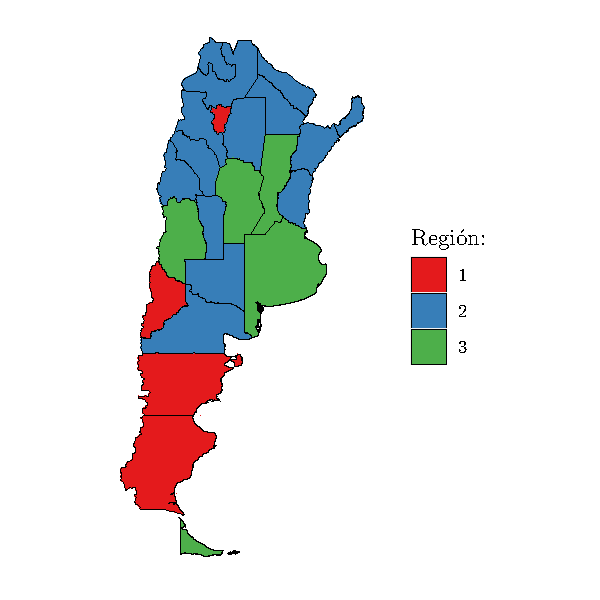
\includegraphics[scale=0.7]{./graficos/mapa_regiones.pdf}
\caption{Mapa de regiones resultantes de la macrolocalización}
\label{figure:mapa_reg}
\end{center}
\end{figure}
\newpage
En la Figura \ref{figure:mapa_reg} se muestra la distribución geográfica de las regiones definidas anteriormente.

Para completar el análisis, en el Cuadro \ref{cuadro:indicadores} se presenta un resumen de los macrofactores que representan en promedio a cada región, es decir, cuales son las características compartidas entre las provincias que provocaron que sean parte de un mismo aglomerado.
\begin{table}[!htbp] 
\center
\footnotesize
\raggedleft
  \caption{Resumen de indicadores por regiones} 
  \label{cuadro:indicadores} 
\begin{tabular}{@{\extracolsep{5pt}} lccc} 
\\[-1.8ex]\hline 
\hline \\[-1.8ex] 
 Indicadores & Region 1 & Region 2 & Region 3 \\ 
\hline \\[-1.8ex] 
 Tasa promocion efectiva secundaria (2017) & $76.25$ & $78.60$ & $82.05$ \\ 
 Mortalidad infantil promedio 2016-2019 & $8.20$ & $9.50$ & $8.25$ \\ 
 Homicidios dolosos C/ 100.000 hab. (2016-2019) & $7.25$ & $3.75$ & $5.30$ \\ 
 Muertes en Accidentes Viales C/ 100.000  hab.  (2016-2019) & $12.40$ & $14.05$ & $7.50$ \\ 
 Robos (no agravados) C/ 100.000 hab. (2016-2019) & $973.40$ & $654.85$ & $1,566.95$ \\ 
 Robos agravados C/ 100.000 hab. (2016-2019) & $27.80$ & $1.70$ & $9.50$ \\ 
 Violaciones  C/ 100.000 hab. (2016-2019) & $15.45$ & $11.15$ & $8.75$ \\ 
 Exportaciones per-cápita en USD (2016-2019) & $2,857.20$ & $794.20$ & $1,420.55$ \\ 
 Demanda de MwH energía elec. Per cápita (2016) & $3.80$ & $2.20$ & $3.35$ \\ 
 Pobreza Promedio (2017-2019) & $26.05$ & $32.55$ & $29.35$ \\ 
 Tasa actividad Promedio (2017-2019) & $44.55$ & $42.50$ & $46$ \\ 
 Empresas  C/ 100.000 hab. (2016-2017) & $1,569.62$ & $846.96$ & $1,771.95$ \\ 
 Remuneracion  real de trabajadores reg. (priv.) (2016-2019) & $29,995.27$ & $14,997.52$ & $17,149.25$ \\ 
 Porcentaje de empleados en sector primario(2016-2019) & $20.70$ & $12.63$ & $4.94$ \\ 
 Porcentaje de empleados en sector terciario (2016-2019) & $66.51$ & $68.89$ & $70.78$ \\ 
 Porcentaje de empleados en sector secundario (2016-2019) & $9.57$ & $15.49$ & $22.38$ 
\\ 
\hline \\[-1.8ex] 

\end{tabular} 
\end{table} 

La \textbf{región 1} se caracteriza en terminos sociales por una tasa de promoción secundaria relativamente baja, en comparación con las otras regiones, una leve mortalidad infantil, una alta tasa de robos agravados, homocidios dolosos y violaciones cada 100.000 habitantes y un nivel moderado de robos no agravados y muertes en accidentes viales cada 100.000 habitantes. En términos económicos, esta región se caracteriza por tener la mejor integración a los mercados internacionales con la mayor cantidad de exportaciones per-cápita. 
En cuanto al nivel de actividad, posee elevados niveles de consumo  de energía electrica per-cápita, la tasa de actividad promedio y la cantidad relativa de empresas es la segunda más elevada de las tres regiones, el salario real es el más alto, con amplia diferencia, de las tres regiones y la tasa de pobreza es la más baja de las tres. Por último, se caracteriza por una predominancia del sector terciario, seguido del sector primario (Agricultura, ganadería, pesca y actividades extractivas) y por último, con un porcentaje considerablemente menor, el sector secundario (industrial).

La \textbf{región 2} se caracteriza en terminos sociales por una moderada tasa de promoción secundaria, en comparación con las otras regiones, una elevada tasa mortalidad infantil, una baja tasa de robos (agravados y no agravados) y homocidios dolosos cada 100.000 habitantes, un nivel moderado de violaciones cada 100.000 habitantes y una elevada tasa de muertes en accidentes viales cada 100.000 habitantes. 
En cuanto a factores económicos, esta región se caracteriza por tener una pésima integración a los mercados internacionales con la más baja cantidad de exportaciones per-cápita, en cuanto a los niveles de actividad, posee los menores niveles de consumo  de energía electrica per-cápita, la menor tasa de actividad promedio, la menor cantidad relativa de empresas, el salario real es el más bajo de las tres regiones y la tasa de pobreza es la más alta de las tres, dejandola en el último puesto en términos de desempeño económico en términos relativos. 
Por último, se caracteriza, al igual que las otras dos regiones, por una predominancia del sector terciario, seguido del sector secundario (industrial) y dejando en último lugar al sector primario (Agricultura, ganadería, pesca y actividades extractivas).

La \textbf{región 3} se caracteriza en terminos sociales por una elevada tasa de promoción secundaria, en comparación con las otras regiones, una moderada tasa mortalidad infantil, muy similar a la región 2, una moderada tasa de robos agravados y homocidios dolosos cada 100.000 habitantes, un nivel bajo en términos relativos de violaciones y muertes en accidentes viales cada 100.000 habitantes y una elevada tasa de robos no agravados. 
En cuanto a factores económicos, esta región se caracteriza por tener un desempeño intermedio en términos de integración a los mercados internacionales, con una cantidad de exportaciones per-cápita en dolares que se encuentra en un término medio entre las dos regiones restantes, en cuanto a los niveles de actividad, posee el segundo mayor nivel de consumo  de energía electrica per-cápita, la mayor tasa de actividad promedio, la mayor cantidad relativa de empresas cada 100.000 habitantes, un nivel intermedio de salario real  y una tasa de pobreza que se encuentra como la segunda más baja de las tres regiones. Por último, se caracteriza, al igual que las otras dos regiones, por una predominancia del sector terciario, seguido del sector secundario (industrial) y dejando en último lugar, con amplia diferencia, al sector primario (Agricultura, ganadería, pesca y actividades extractivas).

\subsection{Flujos migatrorios}

Dentro de las regiones existen provincias de las cuales salen gran cantidad de inmigrantes, al igual que existen provincias que son receptoras de estos mismos, en primer lugar se caracterizará a las regiones según el nivel de \textit{expulsion} de inmigrantes interprovinciales.
\begin{table}[!htbp] \centering 
\footnotesize
  \caption{Regiones de origen de los migrantes} 
  \label{cuadro:origen_mig} 
\begin{tabular}{@{\extracolsep{5pt}} ccc} 
\\[-1.8ex]\hline 
\hline \\[-1.8ex] 
Región & Porcentaje \\ 
\\[-1.8ex]\hline 
\hline \\[-1.8ex] 

 1 & 10.41\%\\ 
 2 & 61.67\%\\ 
 3 & 27.92\%\\ 
\hline \\[-1.8ex] 
\end{tabular} 
\end{table} 
En el Cuadro \ref{cuadro:origen_mig} se puede ntoar que las provincias de la  \textbf{Región Nº2} son las que mayor nivel de expulsión poseen, seguidas por las provincias pertenecientes a la Región Nº3, y por úlitmo se encuentran las pertenecientes a la Región Nº1.

\begin{table}[!htbp] \centering 
\footnotesize
  \caption{Regiones de destino de los migrantes} 
  \label{cuadro:destino_mig} 
\begin{tabular}{@{\extracolsep{5pt}} ccc} 
\\[-1.8ex]\hline 
\hline \\[-1.8ex] 
Región & Porcentaje \\ 
\\[-1.8ex]\hline 
\hline \\[-1.8ex]
1 & 07.85\%\\ 
2 & 12.83\%\\ 
3 & 79.32\%\\ 
\hline \\[-1.8ex] 
\end{tabular} 
\end{table} 

Sin embargo, analizando cuales son las regiones de destino  con mayor porcentaje  de migrantes, se puede encontrar en el Cuadro \ref{cuadro:destino_mig} que la \textbf{Región Nº 3} es la que mayor nivel de *atracción* posee por elevada diferencia (79.32\%), seguida por la Región Nº2 y en último lugar la Región Nº1.

Esta relación entre regiones con mayor atracción y expulsión de migrantes tambien puede ser vista a nivel de provincias, para ello se definen dos tasas a considerar:

\begin{itemize}
\footnotesize
 \item $Tasa\ de\ emigraci\acute{o}n\ de\ la\ Provincia\ "X"= \frac{Cantidad\ de\ migrantes\ nativos\ de\ la\ Provincia\ "X"}{Cantidad\ de\ habitantes\ de\ la\ Provincia\ "X"}$
 \footnotesize 
 \item $Tasa\ de\ inmigraci\acute{o}n\ de\ la\ Provincia\ "X"= \frac{Cantidad\ de\ migrantes\ no\ nativos\  que\ habitan\ la\ Provincia\ "X"}{Cantidad\ de\ habitantes\ de\ la\ Provincia\ "X"}$
\end{itemize}
\begin{figure}[h!]
\begin{center}
% Created by tikzDevice version 0.12.3.1 on 2021-05-21 22:18:04
% !TEX encoding = UTF-8 Unicode
\begin{tikzpicture}[x=1pt,y=1pt]
\definecolor{fillColor}{RGB}{255,255,255}
\path[use as bounding box,fill=fillColor,fill opacity=0.00] (0,0) rectangle (433.62,289.08);
\begin{scope}
\path[clip] (  0.00,  0.00) rectangle (433.62,289.08);
\definecolor{drawColor}{RGB}{255,255,255}
\definecolor{fillColor}{RGB}{255,255,255}

\path[draw=drawColor,line width= 0.6pt,line join=round,line cap=round,fill=fillColor] (  0.00,  0.00) rectangle (433.62,289.08);
\end{scope}
\begin{scope}
\path[clip] ( 26.79, 22.04) rectangle (364.14,266.40);
\definecolor{drawColor}{RGB}{255,255,255}

\path[draw=drawColor,line width= 0.3pt,line join=round] ( 26.79, 62.77) --
	(364.14, 62.77);

\path[draw=drawColor,line width= 0.3pt,line join=round] ( 26.79,122.01) --
	(364.14,122.01);

\path[draw=drawColor,line width= 0.3pt,line join=round] ( 26.79,181.25) --
	(364.14,181.25);

\path[draw=drawColor,line width= 0.3pt,line join=round] ( 26.79,240.49) --
	(364.14,240.49);

\path[draw=drawColor,line width= 0.3pt,line join=round] ( 83.01, 22.04) --
	( 83.01,266.40);

\path[draw=drawColor,line width= 0.3pt,line join=round] (164.79, 22.04) --
	(164.79,266.40);

\path[draw=drawColor,line width= 0.3pt,line join=round] (246.58, 22.04) --
	(246.58,266.40);

\path[draw=drawColor,line width= 0.3pt,line join=round] (328.36, 22.04) --
	(328.36,266.40);

\path[draw=drawColor,line width= 0.6pt,line join=round] ( 26.79, 33.15) --
	(364.14, 33.15);

\path[draw=drawColor,line width= 0.6pt,line join=round] ( 26.79, 92.39) --
	(364.14, 92.39);

\path[draw=drawColor,line width= 0.6pt,line join=round] ( 26.79,151.63) --
	(364.14,151.63);

\path[draw=drawColor,line width= 0.6pt,line join=round] ( 26.79,210.87) --
	(364.14,210.87);

\path[draw=drawColor,line width= 0.6pt,line join=round] ( 42.12, 22.04) --
	( 42.12,266.40);

\path[draw=drawColor,line width= 0.6pt,line join=round] (123.90, 22.04) --
	(123.90,266.40);

\path[draw=drawColor,line width= 0.6pt,line join=round] (205.69, 22.04) --
	(205.69,266.40);

\path[draw=drawColor,line width= 0.6pt,line join=round] (287.47, 22.04) --
	(287.47,266.40);
\definecolor{drawColor}{RGB}{77,175,74}
\definecolor{fillColor}{RGB}{77,175,74}

\path[draw=drawColor,line width= 0.4pt,line join=round,line cap=round,fill=fillColor] ( 82.21, 38.37) circle (  1.96);
\definecolor{drawColor}{RGB}{55,126,184}
\definecolor{fillColor}{RGB}{55,126,184}

\path[draw=drawColor,line width= 0.4pt,line join=round,line cap=round,fill=fillColor] ( 76.90,111.06) circle (  1.96);

\path[draw=drawColor,line width= 0.4pt,line join=round,line cap=round,fill=fillColor] ( 63.50,247.09) circle (  1.96);
\definecolor{drawColor}{RGB}{228,26,28}
\definecolor{fillColor}{RGB}{228,26,28}

\path[draw=drawColor,line width= 0.4pt,line join=round,line cap=round,fill=fillColor] (113.40, 61.30) circle (  1.96);
\definecolor{drawColor}{RGB}{77,175,74}
\definecolor{fillColor}{RGB}{77,175,74}

\path[draw=drawColor,line width= 0.4pt,line join=round,line cap=round,fill=fillColor] ( 80.08, 37.28) circle (  1.96);

\path[draw=drawColor,line width= 0.4pt,line join=round,line cap=round,fill=fillColor] ( 78.84, 63.57) circle (  1.96);
\definecolor{drawColor}{RGB}{55,126,184}
\definecolor{fillColor}{RGB}{55,126,184}

\path[draw=drawColor,line width= 0.4pt,line join=round,line cap=round,fill=fillColor] ( 73.72,220.69) circle (  1.96);

\path[draw=drawColor,line width= 0.4pt,line join=round,line cap=round,fill=fillColor] ( 66.53,195.39) circle (  1.96);

\path[draw=drawColor,line width= 0.4pt,line join=round,line cap=round,fill=fillColor] ( 58.75,132.92) circle (  1.96);

\path[draw=drawColor,line width= 0.4pt,line join=round,line cap=round,fill=fillColor] ( 73.94,111.78) circle (  1.96);

\path[draw=drawColor,line width= 0.4pt,line join=round,line cap=round,fill=fillColor] (104.00,111.07) circle (  1.96);

\path[draw=drawColor,line width= 0.4pt,line join=round,line cap=round,fill=fillColor] ( 93.60, 80.40) circle (  1.96);
\definecolor{drawColor}{RGB}{77,175,74}
\definecolor{fillColor}{RGB}{77,175,74}

\path[draw=drawColor,line width= 0.4pt,line join=round,line cap=round,fill=fillColor] ( 71.56, 62.83) circle (  1.96);
\definecolor{drawColor}{RGB}{55,126,184}
\definecolor{fillColor}{RGB}{55,126,184}

\path[draw=drawColor,line width= 0.4pt,line join=round,line cap=round,fill=fillColor] ( 77.61,148.97) circle (  1.96);
\definecolor{drawColor}{RGB}{228,26,28}
\definecolor{fillColor}{RGB}{228,26,28}

\path[draw=drawColor,line width= 0.4pt,line join=round,line cap=round,fill=fillColor] (124.03, 56.87) circle (  1.96);
\definecolor{drawColor}{RGB}{55,126,184}
\definecolor{fillColor}{RGB}{55,126,184}

\path[draw=drawColor,line width= 0.4pt,line join=round,line cap=round,fill=fillColor] ( 92.65,212.40) circle (  1.96);

\path[draw=drawColor,line width= 0.4pt,line join=round,line cap=round,fill=fillColor] ( 75.42, 87.58) circle (  1.96);

\path[draw=drawColor,line width= 0.4pt,line join=round,line cap=round,fill=fillColor] ( 58.18, 76.60) circle (  1.96);

\path[draw=drawColor,line width= 0.4pt,line join=round,line cap=round,fill=fillColor] (112.49, 76.36) circle (  1.96);
\definecolor{drawColor}{RGB}{228,26,28}
\definecolor{fillColor}{RGB}{228,26,28}

\path[draw=drawColor,line width= 0.4pt,line join=round,line cap=round,fill=fillColor] (143.72, 83.37) circle (  1.96);
\definecolor{drawColor}{RGB}{77,175,74}
\definecolor{fillColor}{RGB}{77,175,74}

\path[draw=drawColor,line width= 0.4pt,line join=round,line cap=round,fill=fillColor] ( 77.75, 60.23) circle (  1.96);
\definecolor{drawColor}{RGB}{55,126,184}
\definecolor{fillColor}{RGB}{55,126,184}

\path[draw=drawColor,line width= 0.4pt,line join=round,line cap=round,fill=fillColor] ( 60.79,201.99) circle (  1.96);
\definecolor{drawColor}{RGB}{77,175,74}
\definecolor{fillColor}{RGB}{77,175,74}

\path[draw=drawColor,line width= 0.4pt,line join=round,line cap=round,fill=fillColor] (204.97, 49.35) circle (  1.96);
\definecolor{drawColor}{RGB}{228,26,28}
\definecolor{fillColor}{RGB}{228,26,28}

\path[draw=drawColor,line width= 0.4pt,line join=round,line cap=round,fill=fillColor] ( 67.48, 98.80) circle (  1.96);
\definecolor{drawColor}{RGB}{0,0,0}

\path[draw=drawColor,line width= 0.6pt,line join=round] ( 26.79, 22.04) -- (364.14,266.40);
\definecolor{drawColor}{RGB}{77,175,74}

\node[text=drawColor,anchor=base,inner sep=0pt, outer sep=0pt, scale=  0.57] at ( 90.17, 42.22) {Buenos Aires};
\definecolor{drawColor}{RGB}{55,126,184}

\node[text=drawColor,anchor=base,inner sep=0pt, outer sep=0pt, scale=  0.57] at ( 89.81,103.30) {Catamarca};

\node[text=drawColor,anchor=base,inner sep=0pt, outer sep=0pt, scale=  0.57] at ( 71.59,250.96) {Chaco};
\definecolor{drawColor}{RGB}{228,26,28}

\node[text=drawColor,anchor=base,inner sep=0pt, outer sep=0pt, scale=  0.57] at (105.42, 53.52) {Chubut};
\definecolor{drawColor}{RGB}{77,175,74}

\node[text=drawColor,anchor=base,inner sep=0pt, outer sep=0pt, scale=  0.57] at ( 73.93, 29.53) {Ciudad Autónoma de Buenos Aires};

\node[text=drawColor,anchor=base,inner sep=0pt, outer sep=0pt, scale=  0.57] at ( 89.16, 67.42) {Córdoba};
\definecolor{drawColor}{RGB}{55,126,184}

\node[text=drawColor,anchor=base,inner sep=0pt, outer sep=0pt, scale=  0.57] at ( 65.65,224.55) {Corrientes};

\node[text=drawColor,anchor=base,inner sep=0pt, outer sep=0pt, scale=  0.57] at ( 74.51,187.64) {Entre Ríos};

\node[text=drawColor,anchor=base,inner sep=0pt, outer sep=0pt, scale=  0.57] at ( 64.29,135.11) {Formosa};

\node[text=drawColor,anchor=base,inner sep=0pt, outer sep=0pt, scale=  0.57] at ( 66.01,115.59) {Jujuy};

\node[text=drawColor,anchor=base,inner sep=0pt, outer sep=0pt, scale=  0.57] at (111.99,114.90) {La Pampa};

\node[text=drawColor,anchor=base,inner sep=0pt, outer sep=0pt, scale=  0.57] at (101.69, 84.31) {La Rioja};
\definecolor{drawColor}{RGB}{77,175,74}

\node[text=drawColor,anchor=base,inner sep=0pt, outer sep=0pt, scale=  0.57] at ( 61.33, 66.71) {Mendoza};
\definecolor{drawColor}{RGB}{55,126,184}

\node[text=drawColor,anchor=base,inner sep=0pt, outer sep=0pt, scale=  0.57] at ( 72.00,142.91) {Misiones};
\definecolor{drawColor}{RGB}{228,26,28}

\node[text=drawColor,anchor=base,inner sep=0pt, outer sep=0pt, scale=  0.57] at (132.05, 49.09) {Neuquén};
\definecolor{drawColor}{RGB}{55,126,184}

\node[text=drawColor,anchor=base,inner sep=0pt, outer sep=0pt, scale=  0.57] at (100.66,204.63) {Río Negro};

\node[text=drawColor,anchor=base,inner sep=0pt, outer sep=0pt, scale=  0.57] at ( 65.08, 91.01) {Salta};

\node[text=drawColor,anchor=base,inner sep=0pt, outer sep=0pt, scale=  0.57] at ( 50.13, 80.49) {San Juan};

\node[text=drawColor,anchor=base,inner sep=0pt, outer sep=0pt, scale=  0.57] at (120.56, 68.58) {San Luis};
\definecolor{drawColor}{RGB}{228,26,28}

\node[text=drawColor,anchor=base,inner sep=0pt, outer sep=0pt, scale=  0.57] at (151.77, 87.27) {Santa Cruz};
\definecolor{drawColor}{RGB}{77,175,74}

\node[text=drawColor,anchor=base,inner sep=0pt, outer sep=0pt, scale=  0.57] at ( 69.80, 52.48) {Santa Fe};
\definecolor{drawColor}{RGB}{55,126,184}

\node[text=drawColor,anchor=base,inner sep=0pt, outer sep=0pt, scale=  0.57] at ( 53.96,205.85) {Santiago del Estero};
\definecolor{drawColor}{RGB}{77,175,74}

\node[text=drawColor,anchor=base,inner sep=0pt, outer sep=0pt, scale=  0.57] at (214.31, 41.49) {Tierra del Fuego, Antártida e Islas del Atlántico Sur};
\definecolor{drawColor}{RGB}{228,26,28}

\node[text=drawColor,anchor=base,inner sep=0pt, outer sep=0pt, scale=  0.57] at ( 58.51,102.70) {Tucumán};
\end{scope}
\begin{scope}
\path[clip] (  0.00,  0.00) rectangle (433.62,289.08);
\definecolor{drawColor}{RGB}{0,0,0}

\path[draw=drawColor,line width= 0.6pt,line join=round] ( 26.79, 22.04) --
	( 26.79,266.40);
\end{scope}
\begin{scope}
\path[clip] (  0.00,  0.00) rectangle (433.62,289.08);
\definecolor{drawColor}{RGB}{0,0,0}

\node[text=drawColor,anchor=base east,inner sep=0pt, outer sep=0pt, scale=  0.50] at ( 21.84, 31.42) {0{\%}};

\node[text=drawColor,anchor=base east,inner sep=0pt, outer sep=0pt, scale=  0.50] at ( 21.84, 90.66) {20{\%}};

\node[text=drawColor,anchor=base east,inner sep=0pt, outer sep=0pt, scale=  0.50] at ( 21.84,149.90) {40{\%}};

\node[text=drawColor,anchor=base east,inner sep=0pt, outer sep=0pt, scale=  0.50] at ( 21.84,209.14) {60{\%}};
\end{scope}
\begin{scope}
\path[clip] (  0.00,  0.00) rectangle (433.62,289.08);
\definecolor{drawColor}{gray}{0.20}

\path[draw=drawColor,line width= 0.6pt,line join=round] ( 24.04, 33.15) --
	( 26.79, 33.15);

\path[draw=drawColor,line width= 0.6pt,line join=round] ( 24.04, 92.39) --
	( 26.79, 92.39);

\path[draw=drawColor,line width= 0.6pt,line join=round] ( 24.04,151.63) --
	( 26.79,151.63);

\path[draw=drawColor,line width= 0.6pt,line join=round] ( 24.04,210.87) --
	( 26.79,210.87);
\end{scope}
\begin{scope}
\path[clip] (  0.00,  0.00) rectangle (433.62,289.08);
\definecolor{drawColor}{RGB}{0,0,0}

\path[draw=drawColor,line width= 0.6pt,line join=round] ( 26.79, 22.04) --
	(364.14, 22.04);
\end{scope}
\begin{scope}
\path[clip] (  0.00,  0.00) rectangle (433.62,289.08);
\definecolor{drawColor}{gray}{0.20}

\path[draw=drawColor,line width= 0.6pt,line join=round] ( 42.12, 19.29) --
	( 42.12, 22.04);

\path[draw=drawColor,line width= 0.6pt,line join=round] (123.90, 19.29) --
	(123.90, 22.04);

\path[draw=drawColor,line width= 0.6pt,line join=round] (205.69, 19.29) --
	(205.69, 22.04);

\path[draw=drawColor,line width= 0.6pt,line join=round] (287.47, 19.29) --
	(287.47, 22.04);
\end{scope}
\begin{scope}
\path[clip] (  0.00,  0.00) rectangle (433.62,289.08);
\definecolor{drawColor}{RGB}{0,0,0}

\node[text=drawColor,anchor=base,inner sep=0pt, outer sep=0pt, scale=  0.50] at ( 42.12, 13.64) {0{\%}};

\node[text=drawColor,anchor=base,inner sep=0pt, outer sep=0pt, scale=  0.50] at (123.90, 13.64) {20{\%}};

\node[text=drawColor,anchor=base,inner sep=0pt, outer sep=0pt, scale=  0.50] at (205.69, 13.64) {40{\%}};

\node[text=drawColor,anchor=base,inner sep=0pt, outer sep=0pt, scale=  0.50] at (287.47, 13.64) {60{\%}};
\end{scope}
\begin{scope}
\path[clip] (  0.00,  0.00) rectangle (433.62,289.08);
\definecolor{drawColor}{RGB}{0,0,0}

\node[text=drawColor,anchor=base,inner sep=0pt, outer sep=0pt, scale=  0.50] at (195.46,  6.47) {\bfseries Tasa de inmigración};
\end{scope}
\begin{scope}
\path[clip] (  0.00,  0.00) rectangle (433.62,289.08);
\definecolor{drawColor}{RGB}{0,0,0}

\node[text=drawColor,rotate= 90.00,anchor=base,inner sep=0pt, outer sep=0pt, scale=  0.50] at (  8.95,144.22) {\bfseries Tasa de emigración};
\end{scope}
\begin{scope}
\path[clip] (  0.00,  0.00) rectangle (433.62,289.08);
\definecolor{fillColor}{RGB}{255,255,255}

\path[fill=fillColor] (375.14,109.43) rectangle (428.12,179.02);
\end{scope}
\begin{scope}
\path[clip] (  0.00,  0.00) rectangle (433.62,289.08);
\definecolor{drawColor}{RGB}{0,0,0}

\node[text=drawColor,anchor=base west,inner sep=0pt, outer sep=0pt, scale=  1.10] at (380.64,164.86) {\bfseries Región:};
\end{scope}
\begin{scope}
\path[clip] (  0.00,  0.00) rectangle (433.62,289.08);
\definecolor{drawColor}{RGB}{228,26,28}
\definecolor{fillColor}{RGB}{228,26,28}

\path[draw=drawColor,line width= 0.4pt,line join=round,line cap=round,fill=fillColor] (387.87,151.06) circle (  1.96);
\end{scope}
\begin{scope}
\path[clip] (  0.00,  0.00) rectangle (433.62,289.08);
\definecolor{drawColor}{RGB}{55,126,184}
\definecolor{fillColor}{RGB}{55,126,184}

\path[draw=drawColor,line width= 0.4pt,line join=round,line cap=round,fill=fillColor] (387.87,136.61) circle (  1.96);
\end{scope}
\begin{scope}
\path[clip] (  0.00,  0.00) rectangle (433.62,289.08);
\definecolor{drawColor}{RGB}{77,175,74}
\definecolor{fillColor}{RGB}{77,175,74}

\path[draw=drawColor,line width= 0.4pt,line join=round,line cap=round,fill=fillColor] (387.87,122.15) circle (  1.96);
\end{scope}
\begin{scope}
\path[clip] (  0.00,  0.00) rectangle (433.62,289.08);
\definecolor{drawColor}{RGB}{0,0,0}

\node[text=drawColor,anchor=base west,inner sep=0pt, outer sep=0pt, scale=  0.88] at (400.59,148.03) {1};
\end{scope}
\begin{scope}
\path[clip] (  0.00,  0.00) rectangle (433.62,289.08);
\definecolor{drawColor}{RGB}{0,0,0}

\node[text=drawColor,anchor=base west,inner sep=0pt, outer sep=0pt, scale=  0.88] at (400.59,133.58) {2};
\end{scope}
\begin{scope}
\path[clip] (  0.00,  0.00) rectangle (433.62,289.08);
\definecolor{drawColor}{RGB}{0,0,0}

\node[text=drawColor,anchor=base west,inner sep=0pt, outer sep=0pt, scale=  0.88] at (400.59,119.12) {3};
\end{scope}
\end{tikzpicture}

\caption{Tasa de inmigración y emigración por provincia}
\label{figure:emig_inmig_prov}
\end{center}
\end{figure}
En la Figura \ref{figure:emig_inmig_prov} se puede observar la relación entre la tasa de emigración e inmigración de las provincias, diferenciando por la región a la cual pertenecen.

La bisectriz divide el plano en dos zonas, todas las provincias que se encuentran por encima de ella son aquellas en la que la tasa de emigración es superior a la tasa de inmigración, mientras que las que se encuentran por debajo, son quellas en la que existe una mayor tasa de inmigración que de emigración. 

Las provincias pertenecientes a la Región Nº2 se ubican en casi su totalidad por encima de la bisectriz, indicando que son provincias en donde la expulsión de migrantes es mucho mayor que la atracción de los mismos, por otro lado, las provincias de la Región Nº 1 tienen una mayor tendencia a ubicarse por debajo de la linea diagonal, en donde la atracción de migrantes es mayor que la expulsión en casi la totalidad de las provincias, con excepción de Tucumán, y por último, en la Región Nº3 se pueden encontrar tres provincias que se encuentran por debajo de la diagonal, en donde la atracción de migrantes es mayor que su nivel de expulsión (Buenos Aires, Ciudad Autónoma de Buenos Aires y Tierra del Fuego) y otras tres que se encuentran con tasa de inmigración y emigración muy similares, con diferencias muy leves a favor de la tasa de emigración.

En la Figura \ref{figure:emig_inmig_prov_mapa} se observa la diferencia en la distribución de las provincias con mayor tasa de migración e inmigración, las provincias de Chaco, Corrientes y Rio Negro son las que mayores tasa de emigración poseen, mientras que en el Sur de la Argentina se encuentran las provincias en donde la tasa de inmigración es mas elevada, con provincias como Tierra del Fuego, Santa Cruz y Neuquén.
\begin{figure}[h!]
\begin{center}
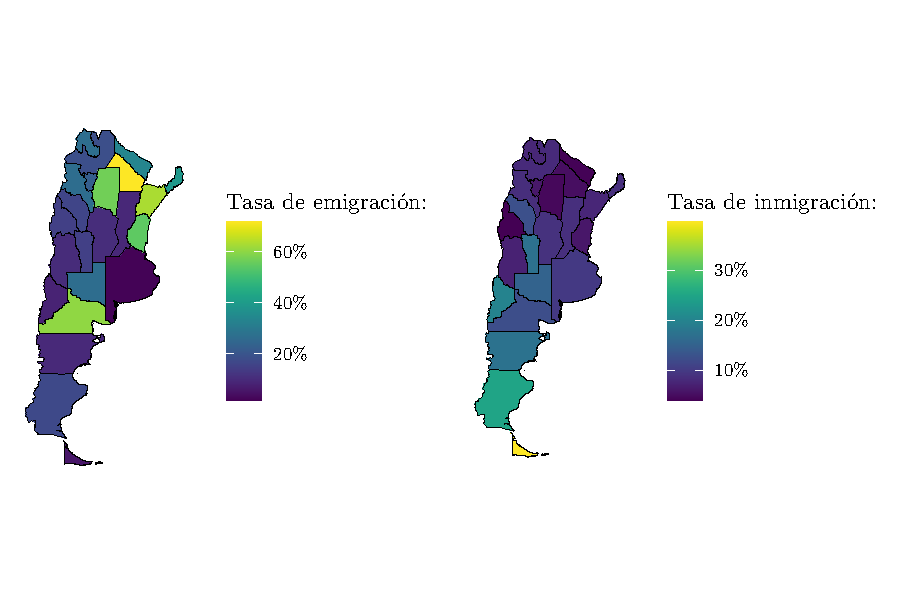
\includegraphics[scale=1.1]{./graficos/emig_inmig_por_prov.pdf}
\caption{Mapa de tasas de emigración e inmigración por provincia}
\label{figure:emig_inmig_prov_mapa}
\end{center}
\end{figure}
\newpage
\section{Migrantes}
Las características individuales o familiares de las personas que toman la decisión de emprender un proceso migratorio forman parte de los microdeterminantes de las migraciones,si bien estas no deben ser tomadas como las principales impulsoras de la decisión del éxodo, funcionan como mediadoras en la decisión migratoria y tienen una elevada influencia en la auto-selección de los migrantes (Borjas, 1987) para cada una de las regiones.

En primer lugar se analizará si existen microdeterminantes dentro de las características de los migrantes que porovoquen que ciertas personas con tengan una mayor propensión a migrar desde ciertas localizaciones, es decir, se analizaran los factores de expulsión de los distintos cluster; por otro lado, se realizará un análisis diferenciando el destino de los distintos migrantes, con el fin de establecer los determinantes de atracción de las distintas localizaciones.

Se tomara como unidad de análisis al Jefe de Hogar, con el fin de condensar la decisión familiar de la migración en un solo sujeto, y reconocer la importancia de los vinculos y las ganancias familiares en las decisiones migratorias de los sujetos (Mincer, 1978).

\subsection{Género y edad}
El género y la edad de las personas son considerados dentro de los microfactores que pueden afectar considerablemente a la decisión migratoria, es por ello que se analizan estas características dentro de la población de cada región, diferenciando entre los que son nativos de la provincia en la que habitan de los que son migrantes.

En la Figura \ref{figure:sexo_mig_} se puede ver el género de los migrantes y nativos de las tres regiones definidas. En las tres regiones los migrantes  son en su mayoría mujeres, siendo la región 3 la que mayor cantidad de migrantes mujeres posee con un $55.62\%$, seguido por la Región 2, y en donde menor cantidad de mujeres migrantes habitan es en la Región 1, con un $52.80\%$ de migrantes mujeres.

Otra particularidad que se puede observar en la Figura \ref{figure:sexo_mig_} es que en todas las regiones la proporción de mujeres nativas es menor que la proporción de mujeres migrantes, esto fenomeno es comunmente conocido en la literatura de migraciones internacionales como feminización de la migración (Carling, 2005), fenomeno que surje, en parte, de la particiación más activa que tomó la mujer en el mercado laboral en las últimas décadas, lo que permitió el acceso a la posibildiad de migrar para formar parte de mercados laborales en donde la valoración de su fuerza de trabajo sea mayor.

\begin{figure}[ht!]
\begin{center}
% Created by tikzDevice version 0.12.3.1 on 2021-05-22 21:10:22
% !TEX encoding = UTF-8 Unicode
\begin{tikzpicture}[x=1pt,y=1pt]
\definecolor{fillColor}{RGB}{255,255,255}
\path[use as bounding box,fill=fillColor,fill opacity=0.00] (0,0) rectangle (433.62,289.08);
\begin{scope}
\path[clip] (  0.00,  0.00) rectangle (433.62,289.08);
\definecolor{drawColor}{RGB}{255,255,255}
\definecolor{fillColor}{RGB}{255,255,255}

\path[draw=drawColor,line width= 0.6pt,line join=round,line cap=round,fill=fillColor] (  0.00,  0.00) rectangle (433.62,289.08);
\end{scope}
\begin{scope}
\path[clip] ( 61.11,202.95) rectangle (335.80,283.58);
\definecolor{drawColor}{RGB}{255,255,255}

\path[draw=drawColor,line width= 0.3pt,line join=round] (104.81,202.95) --
	(104.81,283.58);

\path[draw=drawColor,line width= 0.3pt,line join=round] (167.24,202.95) --
	(167.24,283.58);

\path[draw=drawColor,line width= 0.3pt,line join=round] (229.67,202.95) --
	(229.67,283.58);

\path[draw=drawColor,line width= 0.3pt,line join=round] (292.10,202.95) --
	(292.10,283.58);

\path[draw=drawColor,line width= 0.6pt,line join=round] ( 61.11,224.94) --
	(335.80,224.94);

\path[draw=drawColor,line width= 0.6pt,line join=round] ( 61.11,261.59) --
	(335.80,261.59);

\path[draw=drawColor,line width= 0.6pt,line join=round] ( 73.60,202.95) --
	( 73.60,283.58);

\path[draw=drawColor,line width= 0.6pt,line join=round] (136.03,202.95) --
	(136.03,283.58);

\path[draw=drawColor,line width= 0.6pt,line join=round] (198.45,202.95) --
	(198.45,283.58);

\path[draw=drawColor,line width= 0.6pt,line join=round] (260.88,202.95) --
	(260.88,283.58);

\path[draw=drawColor,line width= 0.6pt,line join=round] (323.31,202.95) --
	(323.31,283.58);
\definecolor{fillColor}{RGB}{228,26,28}

\path[fill=fillColor] (205.44,213.94) rectangle (323.31,235.93);
\definecolor{fillColor}{RGB}{55,126,184}

\path[fill=fillColor] ( 73.60,213.94) rectangle (205.44,235.93);
\definecolor{fillColor}{RGB}{228,26,28}

\path[fill=fillColor] (202.38,250.59) rectangle (323.31,272.58);
\definecolor{fillColor}{RGB}{55,126,184}

\path[fill=fillColor] ( 73.60,250.59) rectangle (202.38,272.58);
\definecolor{drawColor}{RGB}{0,0,0}

\node[text=drawColor,anchor=base,inner sep=0pt, outer sep=0pt, scale=  0.85] at (252.59,222.00) {47.20{\%}};

\node[text=drawColor,anchor=base,inner sep=0pt, outer sep=0pt, scale=  0.85] at (126.33,222.00) {52.80{\%}};

\node[text=drawColor,anchor=base,inner sep=0pt, outer sep=0pt, scale=  0.85] at (250.75,258.65) {48.43{\%}};

\node[text=drawColor,anchor=base,inner sep=0pt, outer sep=0pt, scale=  0.85] at (125.11,258.65) {51.57{\%}};
\end{scope}
\begin{scope}
\path[clip] ( 61.11,116.82) rectangle (335.80,197.45);
\definecolor{drawColor}{RGB}{255,255,255}

\path[draw=drawColor,line width= 0.3pt,line join=round] (104.81,116.82) --
	(104.81,197.45);

\path[draw=drawColor,line width= 0.3pt,line join=round] (167.24,116.82) --
	(167.24,197.45);

\path[draw=drawColor,line width= 0.3pt,line join=round] (229.67,116.82) --
	(229.67,197.45);

\path[draw=drawColor,line width= 0.3pt,line join=round] (292.10,116.82) --
	(292.10,197.45);

\path[draw=drawColor,line width= 0.6pt,line join=round] ( 61.11,138.81) --
	(335.80,138.81);

\path[draw=drawColor,line width= 0.6pt,line join=round] ( 61.11,175.46) --
	(335.80,175.46);

\path[draw=drawColor,line width= 0.6pt,line join=round] ( 73.60,116.82) --
	( 73.60,197.45);

\path[draw=drawColor,line width= 0.6pt,line join=round] (136.03,116.82) --
	(136.03,197.45);

\path[draw=drawColor,line width= 0.6pt,line join=round] (198.45,116.82) --
	(198.45,197.45);

\path[draw=drawColor,line width= 0.6pt,line join=round] (260.88,116.82) --
	(260.88,197.45);

\path[draw=drawColor,line width= 0.6pt,line join=round] (323.31,116.82) --
	(323.31,197.45);
\definecolor{fillColor}{RGB}{228,26,28}

\path[fill=fillColor] (207.27,127.81) rectangle (323.31,149.80);
\definecolor{fillColor}{RGB}{55,126,184}

\path[fill=fillColor] ( 73.60,127.81) rectangle (207.27,149.80);
\definecolor{fillColor}{RGB}{228,26,28}

\path[fill=fillColor] (203.16,164.46) rectangle (323.31,186.45);
\definecolor{fillColor}{RGB}{55,126,184}

\path[fill=fillColor] ( 73.60,164.46) rectangle (203.16,186.45);
\definecolor{drawColor}{RGB}{0,0,0}

\node[text=drawColor,anchor=base,inner sep=0pt, outer sep=0pt, scale=  0.85] at (253.68,135.87) {46.47{\%}};

\node[text=drawColor,anchor=base,inner sep=0pt, outer sep=0pt, scale=  0.85] at (127.07,135.87) {53.53{\%}};

\node[text=drawColor,anchor=base,inner sep=0pt, outer sep=0pt, scale=  0.85] at (251.22,172.52) {48.11{\%}};

\node[text=drawColor,anchor=base,inner sep=0pt, outer sep=0pt, scale=  0.85] at (125.42,172.52) {51.89{\%}};
\end{scope}
\begin{scope}
\path[clip] ( 61.11, 30.69) rectangle (335.80,111.32);
\definecolor{drawColor}{RGB}{255,255,255}

\path[draw=drawColor,line width= 0.3pt,line join=round] (104.81, 30.69) --
	(104.81,111.32);

\path[draw=drawColor,line width= 0.3pt,line join=round] (167.24, 30.69) --
	(167.24,111.32);

\path[draw=drawColor,line width= 0.3pt,line join=round] (229.67, 30.69) --
	(229.67,111.32);

\path[draw=drawColor,line width= 0.3pt,line join=round] (292.10, 30.69) --
	(292.10,111.32);

\path[draw=drawColor,line width= 0.6pt,line join=round] ( 61.11, 52.68) --
	(335.80, 52.68);

\path[draw=drawColor,line width= 0.6pt,line join=round] ( 61.11, 89.33) --
	(335.80, 89.33);

\path[draw=drawColor,line width= 0.6pt,line join=round] ( 73.60, 30.69) --
	( 73.60,111.32);

\path[draw=drawColor,line width= 0.6pt,line join=round] (136.03, 30.69) --
	(136.03,111.32);

\path[draw=drawColor,line width= 0.6pt,line join=round] (198.45, 30.69) --
	(198.45,111.32);

\path[draw=drawColor,line width= 0.6pt,line join=round] (260.88, 30.69) --
	(260.88,111.32);

\path[draw=drawColor,line width= 0.6pt,line join=round] (323.31, 30.69) --
	(323.31,111.32);
\definecolor{fillColor}{RGB}{228,26,28}

\path[fill=fillColor] (212.48, 41.68) rectangle (323.31, 63.67);
\definecolor{fillColor}{RGB}{55,126,184}

\path[fill=fillColor] ( 73.60, 41.68) rectangle (212.48, 63.67);
\definecolor{fillColor}{RGB}{228,26,28}

\path[fill=fillColor] (201.44, 78.33) rectangle (323.31,100.32);
\definecolor{fillColor}{RGB}{55,126,184}

\path[fill=fillColor] ( 73.60, 78.33) rectangle (201.44,100.32);
\definecolor{drawColor}{RGB}{0,0,0}

\node[text=drawColor,anchor=base,inner sep=0pt, outer sep=0pt, scale=  0.85] at (256.81, 49.74) {44.38{\%}};

\node[text=drawColor,anchor=base,inner sep=0pt, outer sep=0pt, scale=  0.85] at (129.15, 49.74) {55.62{\%}};

\node[text=drawColor,anchor=base,inner sep=0pt, outer sep=0pt, scale=  0.85] at (250.19, 86.39) {48.80{\%}};

\node[text=drawColor,anchor=base,inner sep=0pt, outer sep=0pt, scale=  0.85] at (124.74, 86.39) {51.20{\%}};
\end{scope}
\begin{scope}
\path[clip] (335.80,202.95) rectangle (352.37,283.58);
\definecolor{drawColor}{gray}{0.10}

\node[text=drawColor,rotate=-90.00,anchor=base,inner sep=0pt, outer sep=0pt, scale=  0.88] at (341.05,243.26) {\textbf{\{}Región1{\}}};
\end{scope}
\begin{scope}
\path[clip] (335.80,116.82) rectangle (352.37,197.45);
\definecolor{drawColor}{gray}{0.10}

\node[text=drawColor,rotate=-90.00,anchor=base,inner sep=0pt, outer sep=0pt, scale=  0.88] at (341.05,157.13) {\textbf{\{}Región2{\}}};
\end{scope}
\begin{scope}
\path[clip] (335.80, 30.69) rectangle (352.37,111.32);
\definecolor{drawColor}{gray}{0.10}

\node[text=drawColor,rotate=-90.00,anchor=base,inner sep=0pt, outer sep=0pt, scale=  0.88] at (341.05, 71.00) {\textbf{\{}Región3{\}}};
\end{scope}
\begin{scope}
\path[clip] (  0.00,  0.00) rectangle (433.62,289.08);
\definecolor{drawColor}{gray}{0.20}

\path[draw=drawColor,line width= 0.6pt,line join=round] ( 73.60, 27.94) --
	( 73.60, 30.69);

\path[draw=drawColor,line width= 0.6pt,line join=round] (136.03, 27.94) --
	(136.03, 30.69);

\path[draw=drawColor,line width= 0.6pt,line join=round] (198.45, 27.94) --
	(198.45, 30.69);

\path[draw=drawColor,line width= 0.6pt,line join=round] (260.88, 27.94) --
	(260.88, 30.69);

\path[draw=drawColor,line width= 0.6pt,line join=round] (323.31, 27.94) --
	(323.31, 30.69);
\end{scope}
\begin{scope}
\path[clip] (  0.00,  0.00) rectangle (433.62,289.08);
\definecolor{drawColor}{RGB}{0,0,0}

\node[text=drawColor,anchor=base,inner sep=0pt, outer sep=0pt, scale=  0.88] at ( 73.60, 19.68) {0{\%}};

\node[text=drawColor,anchor=base,inner sep=0pt, outer sep=0pt, scale=  0.88] at (136.03, 19.68) {25{\%}};

\node[text=drawColor,anchor=base,inner sep=0pt, outer sep=0pt, scale=  0.88] at (198.45, 19.68) {50{\%}};

\node[text=drawColor,anchor=base,inner sep=0pt, outer sep=0pt, scale=  0.88] at (260.88, 19.68) {75{\%}};

\node[text=drawColor,anchor=base,inner sep=0pt, outer sep=0pt, scale=  0.88] at (323.31, 19.68) {100{\%}};
\end{scope}
\begin{scope}
\path[clip] (  0.00,  0.00) rectangle (433.62,289.08);
\definecolor{drawColor}{RGB}{0,0,0}

\node[text=drawColor,anchor=base east,inner sep=0pt, outer sep=0pt, scale=  0.88] at ( 56.16,221.91) {Migrantes};

\node[text=drawColor,anchor=base east,inner sep=0pt, outer sep=0pt, scale=  0.88] at ( 56.16,258.56) {Nativos};
\end{scope}
\begin{scope}
\path[clip] (  0.00,  0.00) rectangle (433.62,289.08);
\definecolor{drawColor}{gray}{0.20}

\path[draw=drawColor,line width= 0.6pt,line join=round] ( 58.36,224.94) --
	( 61.11,224.94);

\path[draw=drawColor,line width= 0.6pt,line join=round] ( 58.36,261.59) --
	( 61.11,261.59);
\end{scope}
\begin{scope}
\path[clip] (  0.00,  0.00) rectangle (433.62,289.08);
\definecolor{drawColor}{RGB}{0,0,0}

\node[text=drawColor,anchor=base east,inner sep=0pt, outer sep=0pt, scale=  0.88] at ( 56.16,135.78) {Migrantes};

\node[text=drawColor,anchor=base east,inner sep=0pt, outer sep=0pt, scale=  0.88] at ( 56.16,172.43) {Nativos};
\end{scope}
\begin{scope}
\path[clip] (  0.00,  0.00) rectangle (433.62,289.08);
\definecolor{drawColor}{gray}{0.20}

\path[draw=drawColor,line width= 0.6pt,line join=round] ( 58.36,138.81) --
	( 61.11,138.81);

\path[draw=drawColor,line width= 0.6pt,line join=round] ( 58.36,175.46) --
	( 61.11,175.46);
\end{scope}
\begin{scope}
\path[clip] (  0.00,  0.00) rectangle (433.62,289.08);
\definecolor{drawColor}{RGB}{0,0,0}

\node[text=drawColor,anchor=base east,inner sep=0pt, outer sep=0pt, scale=  0.88] at ( 56.16, 49.65) {Migrantes};

\node[text=drawColor,anchor=base east,inner sep=0pt, outer sep=0pt, scale=  0.88] at ( 56.16, 86.30) {Nativos};
\end{scope}
\begin{scope}
\path[clip] (  0.00,  0.00) rectangle (433.62,289.08);
\definecolor{drawColor}{gray}{0.20}

\path[draw=drawColor,line width= 0.6pt,line join=round] ( 58.36, 52.68) --
	( 61.11, 52.68);

\path[draw=drawColor,line width= 0.6pt,line join=round] ( 58.36, 89.33) --
	( 61.11, 89.33);
\end{scope}
\begin{scope}
\path[clip] (  0.00,  0.00) rectangle (433.62,289.08);
\definecolor{fillColor}{RGB}{255,255,255}

\path[fill=fillColor] (363.37,129.57) rectangle (428.12,184.69);
\end{scope}
\begin{scope}
\path[clip] (  0.00,  0.00) rectangle (433.62,289.08);
\definecolor{fillColor}{gray}{0.95}

\path[fill=fillColor] (368.87,149.53) rectangle (383.32,163.98);
\end{scope}
\begin{scope}
\path[clip] (  0.00,  0.00) rectangle (433.62,289.08);
\definecolor{fillColor}{RGB}{228,26,28}

\path[fill=fillColor] (369.58,150.24) rectangle (382.61,163.27);
\end{scope}
\begin{scope}
\path[clip] (  0.00,  0.00) rectangle (433.62,289.08);
\definecolor{fillColor}{gray}{0.95}

\path[fill=fillColor] (368.87,135.07) rectangle (383.32,149.53);
\end{scope}
\begin{scope}
\path[clip] (  0.00,  0.00) rectangle (433.62,289.08);
\definecolor{fillColor}{RGB}{55,126,184}

\path[fill=fillColor] (369.58,135.78) rectangle (382.61,148.81);
\end{scope}
\begin{scope}
\path[clip] (  0.00,  0.00) rectangle (433.62,289.08);
\definecolor{drawColor}{RGB}{0,0,0}

\node[text=drawColor,anchor=base west,inner sep=0pt, outer sep=0pt, scale=  0.88] at (388.82,153.72) {Hombres};
\end{scope}
\begin{scope}
\path[clip] (  0.00,  0.00) rectangle (433.62,289.08);
\definecolor{drawColor}{RGB}{0,0,0}

\node[text=drawColor,anchor=base west,inner sep=0pt, outer sep=0pt, scale=  0.88] at (388.82,139.27) {Mujeres};
\end{scope}
\end{tikzpicture}
 
 	\caption{Género de los nativos y migrantes}
 	\label{figure:sexo_mig_}
	\source{Elaboración propia en base a EPH}
\end{center}

\end{figure}

\newpage
En la Figura \ref{figure:edad_mig} se puede observar función de densidad de la edad de los nativos y migrantes de cada una de las tres regiones, la distribución de la edad de los nativos  está desplazada y centrada en valores de edad considerablemente menores que la de los migrantes, y esta relación se cumple para las tres regiones, sin embargo, es más notoria para la región 3 en donde la vejez de la población migrante difiere considerablemente de las características etárias de la población nativa, la cual deja entrever una población menos avejentada en términos relativos.

La teoría clásica ve a la migración como una inversión en capital humano, siguiendo esta linea, un individuo calcula el valor actual descontado del flujo de ganancias de por vida esperado en su región de origen y en la región a la que proyecta migrar, y tomará la decisión del éxodo solamente si el retorno neto de los ``costos de migrar'' son mayores en la localidad de destino que en su localidad de origen (Zaiceva 2014). De acuerdo con esta teoría, mientras mas joven es el migrante, mas largo es el horizonte de vida proyectado y por ende sus ganancias esperadas, y mientras más viejo sea el migrante, no solo este horizonte esperado en el que podra realizar sus ganancias es menor, sino que también seran mayores  los ``costos de migrar'', como por ejemplo los costos psicologicos de separarse de familia y amigos, el mayor capital social que deberán dejar atras, la dificultad de integrarse en una nueva cultura, entre otros.

Como se puede observar en el Cuadro \ref{cuadro:edad_mig}, la mitad de los migrantes en las regiones 1 y 2 se encuentra en torno a los 40 a 45 años, sin embargo, esta relación no se cumple para la región 3, en la cual la mediana de la edad de los migrantes se encuentra en edad mayores a los 50 años, siendo considerablemente mayor a la edad mediana de la población nativa.

Este fenomeno conocido como ``avejentamiento de la migración'' (Zacieva 2014) viene de la mano de una reducción de la migración de personas en edad laboral por falta de demandas laborales atractivas que impliquen un diferencial en las ganancias de los migrantes y que justifiquen los costos de las migraciones.
\begin{figure}[ht!]
\begin{center}
% Created by tikzDevice version 0.12.3.1 on 2021-07-01 11:54:32
% !TEX encoding = UTF-8 Unicode
\begin{tikzpicture}[x=1pt,y=1pt]
\definecolor{fillColor}{RGB}{255,255,255}
\path[use as bounding box,fill=fillColor,fill opacity=0.00] (0,0) rectangle (433.62,289.08);
\begin{scope}
\path[clip] (  0.00,  0.00) rectangle (433.62,289.08);
\definecolor{drawColor}{RGB}{255,255,255}
\definecolor{fillColor}{RGB}{255,255,255}

\path[draw=drawColor,line width= 0.6pt,line join=round,line cap=round,fill=fillColor] (  0.00, -0.00) rectangle (433.62,289.08);
\end{scope}
\begin{scope}
\path[clip] ( 41.49, 67.14) rectangle (166.70,267.01);
\definecolor{drawColor}{RGB}{255,255,255}

\path[draw=drawColor,line width= 0.3pt,line join=round] ( 41.49,104.00) --
	(166.70,104.00);

\path[draw=drawColor,line width= 0.3pt,line join=round] ( 41.49,159.56) --
	(166.70,159.56);

\path[draw=drawColor,line width= 0.3pt,line join=round] ( 41.49,215.11) --
	(166.70,215.11);

\path[draw=drawColor,line width= 0.3pt,line join=round] ( 52.87, 67.14) --
	( 52.87,267.01);

\path[draw=drawColor,line width= 0.3pt,line join=round] ( 87.02, 67.14) --
	( 87.02,267.01);

\path[draw=drawColor,line width= 0.3pt,line join=round] (121.17, 67.14) --
	(121.17,267.01);

\path[draw=drawColor,line width= 0.3pt,line join=round] (155.32, 67.14) --
	(155.32,267.01);

\path[draw=drawColor,line width= 0.6pt,line join=round] ( 41.49, 76.22) --
	(166.70, 76.22);

\path[draw=drawColor,line width= 0.6pt,line join=round] ( 41.49,131.78) --
	(166.70,131.78);

\path[draw=drawColor,line width= 0.6pt,line join=round] ( 41.49,187.33) --
	(166.70,187.33);

\path[draw=drawColor,line width= 0.6pt,line join=round] ( 41.49,242.89) --
	(166.70,242.89);

\path[draw=drawColor,line width= 0.6pt,line join=round] ( 69.94, 67.14) --
	( 69.94,267.01);

\path[draw=drawColor,line width= 0.6pt,line join=round] (104.09, 67.14) --
	(104.09,267.01);

\path[draw=drawColor,line width= 0.6pt,line join=round] (138.24, 67.14) --
	(138.24,267.01);
\definecolor{fillColor}{RGB}{228,26,28}

\path[fill=fillColor,fill opacity=0.50] ( 47.18, 76.25) --
	( 47.40, 76.26) --
	( 47.62, 76.28) --
	( 47.85, 76.30) --
	( 48.07, 76.33) --
	( 48.29, 76.37) --
	( 48.52, 76.42) --
	( 48.74, 76.49) --
	( 48.96, 76.58) --
	( 49.18, 76.69) --
	( 49.41, 76.84) --
	( 49.63, 77.04) --
	( 49.85, 77.29) --
	( 50.07, 77.60) --
	( 50.30, 77.99) --
	( 50.52, 78.46) --
	( 50.74, 79.04) --
	( 50.97, 79.76) --
	( 51.19, 80.64) --
	( 51.41, 81.69) --
	( 51.63, 82.93) --
	( 51.86, 84.39) --
	( 52.08, 86.09) --
	( 52.30, 88.06) --
	( 52.53, 90.38) --
	( 52.75, 93.03) --
	( 52.97, 96.03) --
	( 53.19, 99.38) --
	( 53.42,103.12) --
	( 53.64,107.25) --
	( 53.86,111.79) --
	( 54.08,116.80) --
	( 54.31,122.20) --
	( 54.53,127.99) --
	( 54.75,134.13) --
	( 54.98,140.62) --
	( 55.20,147.40) --
	( 55.42,154.47) --
	( 55.64,161.77) --
	( 55.87,169.21) --
	( 56.09,176.74) --
	( 56.31,184.30) --
	( 56.53,191.82) --
	( 56.76,199.25) --
	( 56.98,206.48) --
	( 57.20,213.43) --
	( 57.43,220.07) --
	( 57.65,226.32) --
	( 57.87,232.13) --
	( 58.09,237.46) --
	( 58.32,242.27) --
	( 58.54,246.43) --
	( 58.76,249.93) --
	( 58.99,252.81) --
	( 59.21,255.05) --
	( 59.43,256.64) --
	( 59.65,257.60) --
	( 59.88,257.92) --
	( 60.10,257.54) --
	( 60.32,256.56) --
	( 60.54,255.05) --
	( 60.77,253.04) --
	( 60.99,250.58) --
	( 61.21,247.71) --
	( 61.44,244.49) --
	( 61.66,240.91) --
	( 61.88,237.12) --
	( 62.10,233.15) --
	( 62.33,229.07) --
	( 62.55,224.92) --
	( 62.77,220.74) --
	( 62.99,216.58) --
	( 63.22,212.51) --
	( 63.44,208.54) --
	( 63.66,204.70) --
	( 63.89,201.02) --
	( 64.11,197.50) --
	( 64.33,194.16) --
	( 64.55,191.03) --
	( 64.78,188.10) --
	( 65.00,185.36) --
	( 65.22,182.79) --
	( 65.44,180.38) --
	( 65.67,178.11) --
	( 65.89,175.99) --
	( 66.11,173.99) --
	( 66.34,172.09) --
	( 66.56,170.27) --
	( 66.78,168.52) --
	( 67.00,166.81) --
	( 67.23,165.14) --
	( 67.45,163.49) --
	( 67.67,161.87) --
	( 67.90,160.25) --
	( 68.12,158.63) --
	( 68.34,157.02) --
	( 68.56,155.42) --
	( 68.79,153.82) --
	( 69.01,152.22) --
	( 69.23,150.65) --
	( 69.45,149.10) --
	( 69.68,147.58) --
	( 69.90,146.09) --
	( 70.12,144.65) --
	( 70.35,143.26) --
	( 70.57,141.92) --
	( 70.79,140.65) --
	( 71.01,139.44) --
	( 71.24,138.31) --
	( 71.46,137.24) --
	( 71.68,136.25) --
	( 71.90,135.32) --
	( 72.13,134.47) --
	( 72.35,133.69) --
	( 72.57,132.97) --
	( 72.80,132.31) --
	( 73.02,131.70) --
	( 73.24,131.14) --
	( 73.46,130.62) --
	( 73.69,130.13) --
	( 73.91,129.66) --
	( 74.13,129.21) --
	( 74.36,128.77) --
	( 74.58,128.33) --
	( 74.80,127.88) --
	( 75.02,127.42) --
	( 75.25,126.93) --
	( 75.47,126.42) --
	( 75.69,125.88) --
	( 75.91,125.31) --
	( 76.14,124.69) --
	( 76.36,124.05) --
	( 76.58,123.36) --
	( 76.81,122.63) --
	( 77.03,121.86) --
	( 77.25,121.07) --
	( 77.47,120.24) --
	( 77.70,119.39) --
	( 77.92,118.52) --
	( 78.14,117.63) --
	( 78.36,116.74) --
	( 78.59,115.85) --
	( 78.81,114.96) --
	( 79.03,114.08) --
	( 79.26,113.22) --
	( 79.48,112.39) --
	( 79.70,111.58) --
	( 79.92,110.81) --
	( 80.15,110.07) --
	( 80.37,109.38) --
	( 80.59,108.72) --
	( 80.82,108.10) --
	( 81.04,107.53) --
	( 81.26,107.00) --
	( 81.48,106.51) --
	( 81.71,106.06) --
	( 81.93,105.65) --
	( 82.15,105.27) --
	( 82.37,104.92) --
	( 82.60,104.60) --
	( 82.82,104.30) --
	( 83.04,104.02) --
	( 83.27,103.77) --
	( 83.49,103.52) --
	( 83.71,103.29) --
	( 83.93,103.06) --
	( 84.16,102.84) --
	( 84.38,102.62) --
	( 84.60,102.40) --
	( 84.82,102.17) --
	( 85.05,101.94) --
	( 85.27,101.71) --
	( 85.49,101.47) --
	( 85.72,101.21) --
	( 85.94,100.95) --
	( 86.16,100.68) --
	( 86.38,100.39) --
	( 86.61,100.09) --
	( 86.83, 99.78) --
	( 87.05, 99.46) --
	( 87.28, 99.13) --
	( 87.50, 98.78) --
	( 87.72, 98.43) --
	( 87.94, 98.07) --
	( 88.17, 97.70) --
	( 88.39, 97.32) --
	( 88.61, 96.95) --
	( 88.83, 96.57) --
	( 89.06, 96.19) --
	( 89.28, 95.82) --
	( 89.50, 95.45) --
	( 89.73, 95.10) --
	( 89.95, 94.76) --
	( 90.17, 94.43) --
	( 90.39, 94.11) --
	( 90.62, 93.82) --
	( 90.84, 93.54) --
	( 91.06, 93.29) --
	( 91.28, 93.06) --
	( 91.51, 92.84) --
	( 91.73, 92.65) --
	( 91.95, 92.47) --
	( 92.18, 92.32) --
	( 92.40, 92.18) --
	( 92.62, 92.05) --
	( 92.84, 91.93) --
	( 93.07, 91.83) --
	( 93.29, 91.73) --
	( 93.51, 91.64) --
	( 93.73, 91.54) --
	( 93.96, 91.45) --
	( 94.18, 91.36) --
	( 94.40, 91.26) --
	( 94.63, 91.16) --
	( 94.85, 91.06) --
	( 95.07, 90.95) --
	( 95.29, 90.83) --
	( 95.52, 90.71) --
	( 95.74, 90.59) --
	( 95.96, 90.46) --
	( 96.19, 90.33) --
	( 96.41, 90.20) --
	( 96.63, 90.07) --
	( 96.85, 89.94) --
	( 97.08, 89.82) --
	( 97.30, 89.69) --
	( 97.52, 89.57) --
	( 97.74, 89.45) --
	( 97.97, 89.34) --
	( 98.19, 89.23) --
	( 98.41, 89.13) --
	( 98.64, 89.03) --
	( 98.86, 88.94) --
	( 99.08, 88.85) --
	( 99.30, 88.76) --
	( 99.53, 88.68) --
	( 99.75, 88.61) --
	( 99.97, 88.54) --
	(100.19, 88.48) --
	(100.42, 88.42) --
	(100.64, 88.37) --
	(100.86, 88.33) --
	(101.09, 88.29) --
	(101.31, 88.26) --
	(101.53, 88.23) --
	(101.75, 88.21) --
	(101.98, 88.20) --
	(102.20, 88.18) --
	(102.42, 88.18) --
	(102.65, 88.18) --
	(102.87, 88.18) --
	(103.09, 88.18) --
	(103.31, 88.19) --
	(103.54, 88.20) --
	(103.76, 88.22) --
	(103.98, 88.23) --
	(104.20, 88.25) --
	(104.43, 88.28) --
	(104.65, 88.31) --
	(104.87, 88.34) --
	(105.10, 88.38) --
	(105.32, 88.43) --
	(105.54, 88.48) --
	(105.76, 88.53) --
	(105.99, 88.59) --
	(106.21, 88.65) --
	(106.43, 88.71) --
	(106.65, 88.78) --
	(106.88, 88.84) --
	(107.10, 88.89) --
	(107.32, 88.94) --
	(107.55, 88.97) --
	(107.77, 88.99) --
	(107.99, 88.99) --
	(108.21, 88.97) --
	(108.44, 88.93) --
	(108.66, 88.87) --
	(108.88, 88.78) --
	(109.11, 88.66) --
	(109.33, 88.52) --
	(109.55, 88.35) --
	(109.77, 88.16) --
	(110.00, 87.94) --
	(110.22, 87.71) --
	(110.44, 87.46) --
	(110.66, 87.19) --
	(110.89, 86.91) --
	(111.11, 86.62) --
	(111.33, 86.33) --
	(111.56, 86.04) --
	(111.78, 85.75) --
	(112.00, 85.46) --
	(112.22, 85.19) --
	(112.45, 84.92) --
	(112.67, 84.67) --
	(112.89, 84.42) --
	(113.11, 84.19) --
	(113.34, 83.98) --
	(113.56, 83.78) --
	(113.78, 83.60) --
	(114.01, 83.43) --
	(114.23, 83.28) --
	(114.45, 83.14) --
	(114.67, 83.01) --
	(114.90, 82.90) --
	(115.12, 82.80) --
	(115.34, 82.71) --
	(115.56, 82.63) --
	(115.79, 82.56) --
	(116.01, 82.50) --
	(116.23, 82.44) --
	(116.46, 82.41) --
	(116.68, 82.38) --
	(116.90, 82.36) --
	(117.12, 82.35) --
	(117.35, 82.35) --
	(117.57, 82.36) --
	(117.79, 82.39) --
	(118.02, 82.42) --
	(118.24, 82.46) --
	(118.46, 82.51) --
	(118.68, 82.56) --
	(118.91, 82.62) --
	(119.13, 82.68) --
	(119.35, 82.75) --
	(119.57, 82.81) --
	(119.80, 82.86) --
	(120.02, 82.91) --
	(120.24, 82.95) --
	(120.47, 82.98) --
	(120.69, 83.00) --
	(120.91, 83.01) --
	(121.13, 83.00) --
	(121.36, 82.97) --
	(121.58, 82.93) --
	(121.80, 82.88) --
	(122.02, 82.81) --
	(122.25, 82.72) --
	(122.47, 82.62) --
	(122.69, 82.51) --
	(122.92, 82.39) --
	(123.14, 82.26) --
	(123.36, 82.13) --
	(123.58, 81.98) --
	(123.81, 81.83) --
	(124.03, 81.68) --
	(124.25, 81.53) --
	(124.48, 81.38) --
	(124.70, 81.23) --
	(124.92, 81.08) --
	(125.14, 80.94) --
	(125.37, 80.80) --
	(125.59, 80.66) --
	(125.81, 80.53) --
	(126.03, 80.41) --
	(126.26, 80.30) --
	(126.48, 80.19) --
	(126.70, 80.08) --
	(126.93, 79.99) --
	(127.15, 79.90) --
	(127.37, 79.83) --
	(127.59, 79.76) --
	(127.82, 79.70) --
	(128.04, 79.65) --
	(128.26, 79.60) --
	(128.48, 79.57) --
	(128.71, 79.55) --
	(128.93, 79.53) --
	(129.15, 79.53) --
	(129.38, 79.53) --
	(129.60, 79.55) --
	(129.82, 79.57) --
	(130.04, 79.60) --
	(130.27, 79.63) --
	(130.49, 79.68) --
	(130.71, 79.72) --
	(130.94, 79.77) --
	(131.16, 79.82) --
	(131.38, 79.88) --
	(131.60, 79.93) --
	(131.83, 79.97) --
	(132.05, 80.02) --
	(132.27, 80.05) --
	(132.49, 80.08) --
	(132.72, 80.10) --
	(132.94, 80.10) --
	(133.16, 80.09) --
	(133.39, 80.07) --
	(133.61, 80.04) --
	(133.83, 79.99) --
	(134.05, 79.93) --
	(134.28, 79.85) --
	(134.50, 79.77) --
	(134.72, 79.67) --
	(134.94, 79.56) --
	(135.17, 79.44) --
	(135.39, 79.32) --
	(135.61, 79.19) --
	(135.84, 79.05) --
	(136.06, 78.92) --
	(136.28, 78.78) --
	(136.50, 78.65) --
	(136.73, 78.52) --
	(136.95, 78.39) --
	(137.17, 78.26) --
	(137.39, 78.14) --
	(137.62, 78.03) --
	(137.84, 77.92) --
	(138.06, 77.82) --
	(138.29, 77.73) --
	(138.51, 77.64) --
	(138.73, 77.56) --
	(138.95, 77.48) --
	(139.18, 77.41) --
	(139.40, 77.34) --
	(139.62, 77.28) --
	(139.85, 77.22) --
	(140.07, 77.16) --
	(140.29, 77.10) --
	(140.51, 77.05) --
	(140.74, 77.00) --
	(140.96, 76.95) --
	(141.18, 76.90) --
	(141.40, 76.85) --
	(141.63, 76.80) --
	(141.85, 76.76) --
	(142.07, 76.71) --
	(142.30, 76.67) --
	(142.52, 76.63) --
	(142.74, 76.59) --
	(142.96, 76.55) --
	(143.19, 76.52) --
	(143.41, 76.49) --
	(143.63, 76.45) --
	(143.85, 76.43) --
	(144.08, 76.40) --
	(144.30, 76.38) --
	(144.52, 76.35) --
	(144.75, 76.33) --
	(144.97, 76.32) --
	(145.19, 76.30) --
	(145.41, 76.29) --
	(145.64, 76.28) --
	(145.86, 76.27) --
	(146.08, 76.26) --
	(146.31, 76.25) --
	(146.53, 76.25) --
	(146.75, 76.24) --
	(146.97, 76.24) --
	(147.20, 76.24) --
	(147.42, 76.23) --
	(147.64, 76.23) --
	(147.86, 76.23) --
	(148.09, 76.23) --
	(148.31, 76.23) --
	(148.53, 76.23) --
	(148.76, 76.23) --
	(148.98, 76.23) --
	(149.20, 76.23) --
	(149.42, 76.23) --
	(149.65, 76.23) --
	(149.87, 76.23) --
	(150.09, 76.22) --
	(150.31, 76.22) --
	(150.54, 76.22) --
	(150.76, 76.22) --
	(150.98, 76.22) --
	(151.21, 76.22) --
	(151.43, 76.22) --
	(151.65, 76.22) --
	(151.87, 76.22) --
	(152.10, 76.22) --
	(152.32, 76.22) --
	(152.54, 76.22) --
	(152.77, 76.22) --
	(152.99, 76.22) --
	(153.21, 76.22) --
	(153.43, 76.22) --
	(153.66, 76.22) --
	(153.88, 76.22) --
	(154.10, 76.22) --
	(154.32, 76.22) --
	(154.55, 76.22) --
	(154.77, 76.22) --
	(154.99, 76.22) --
	(155.22, 76.22) --
	(155.44, 76.22) --
	(155.66, 76.22) --
	(155.88, 76.22) --
	(156.11, 76.22) --
	(156.33, 76.22) --
	(156.55, 76.22) --
	(156.77, 76.22) --
	(157.00, 76.22) --
	(157.22, 76.22) --
	(157.44, 76.22) --
	(157.67, 76.22) --
	(157.89, 76.22) --
	(158.11, 76.22) --
	(158.33, 76.22) --
	(158.56, 76.22) --
	(158.78, 76.22) --
	(159.00, 76.22) --
	(159.22, 76.22) --
	(159.45, 76.22) --
	(159.67, 76.22) --
	(159.89, 76.22) --
	(160.12, 76.22) --
	(160.34, 76.22) --
	(160.56, 76.22) --
	(160.78, 76.22) --
	(161.01, 76.22) --
	(161.01, 76.22) --
	(160.78, 76.22) --
	(160.56, 76.22) --
	(160.34, 76.22) --
	(160.12, 76.22) --
	(159.89, 76.22) --
	(159.67, 76.22) --
	(159.45, 76.22) --
	(159.22, 76.22) --
	(159.00, 76.22) --
	(158.78, 76.22) --
	(158.56, 76.22) --
	(158.33, 76.22) --
	(158.11, 76.22) --
	(157.89, 76.22) --
	(157.67, 76.22) --
	(157.44, 76.22) --
	(157.22, 76.22) --
	(157.00, 76.22) --
	(156.77, 76.22) --
	(156.55, 76.22) --
	(156.33, 76.22) --
	(156.11, 76.22) --
	(155.88, 76.22) --
	(155.66, 76.22) --
	(155.44, 76.22) --
	(155.22, 76.22) --
	(154.99, 76.22) --
	(154.77, 76.22) --
	(154.55, 76.22) --
	(154.32, 76.22) --
	(154.10, 76.22) --
	(153.88, 76.22) --
	(153.66, 76.22) --
	(153.43, 76.22) --
	(153.21, 76.22) --
	(152.99, 76.22) --
	(152.77, 76.22) --
	(152.54, 76.22) --
	(152.32, 76.22) --
	(152.10, 76.22) --
	(151.87, 76.22) --
	(151.65, 76.22) --
	(151.43, 76.22) --
	(151.21, 76.22) --
	(150.98, 76.22) --
	(150.76, 76.22) --
	(150.54, 76.22) --
	(150.31, 76.22) --
	(150.09, 76.22) --
	(149.87, 76.22) --
	(149.65, 76.22) --
	(149.42, 76.22) --
	(149.20, 76.22) --
	(148.98, 76.22) --
	(148.76, 76.22) --
	(148.53, 76.22) --
	(148.31, 76.22) --
	(148.09, 76.22) --
	(147.86, 76.22) --
	(147.64, 76.22) --
	(147.42, 76.22) --
	(147.20, 76.22) --
	(146.97, 76.22) --
	(146.75, 76.22) --
	(146.53, 76.22) --
	(146.31, 76.22) --
	(146.08, 76.22) --
	(145.86, 76.22) --
	(145.64, 76.22) --
	(145.41, 76.22) --
	(145.19, 76.22) --
	(144.97, 76.22) --
	(144.75, 76.22) --
	(144.52, 76.22) --
	(144.30, 76.22) --
	(144.08, 76.22) --
	(143.85, 76.22) --
	(143.63, 76.22) --
	(143.41, 76.22) --
	(143.19, 76.22) --
	(142.96, 76.22) --
	(142.74, 76.22) --
	(142.52, 76.22) --
	(142.30, 76.22) --
	(142.07, 76.22) --
	(141.85, 76.22) --
	(141.63, 76.22) --
	(141.40, 76.22) --
	(141.18, 76.22) --
	(140.96, 76.22) --
	(140.74, 76.22) --
	(140.51, 76.22) --
	(140.29, 76.22) --
	(140.07, 76.22) --
	(139.85, 76.22) --
	(139.62, 76.22) --
	(139.40, 76.22) --
	(139.18, 76.22) --
	(138.95, 76.22) --
	(138.73, 76.22) --
	(138.51, 76.22) --
	(138.29, 76.22) --
	(138.06, 76.22) --
	(137.84, 76.22) --
	(137.62, 76.22) --
	(137.39, 76.22) --
	(137.17, 76.22) --
	(136.95, 76.22) --
	(136.73, 76.22) --
	(136.50, 76.22) --
	(136.28, 76.22) --
	(136.06, 76.22) --
	(135.84, 76.22) --
	(135.61, 76.22) --
	(135.39, 76.22) --
	(135.17, 76.22) --
	(134.94, 76.22) --
	(134.72, 76.22) --
	(134.50, 76.22) --
	(134.28, 76.22) --
	(134.05, 76.22) --
	(133.83, 76.22) --
	(133.61, 76.22) --
	(133.39, 76.22) --
	(133.16, 76.22) --
	(132.94, 76.22) --
	(132.72, 76.22) --
	(132.49, 76.22) --
	(132.27, 76.22) --
	(132.05, 76.22) --
	(131.83, 76.22) --
	(131.60, 76.22) --
	(131.38, 76.22) --
	(131.16, 76.22) --
	(130.94, 76.22) --
	(130.71, 76.22) --
	(130.49, 76.22) --
	(130.27, 76.22) --
	(130.04, 76.22) --
	(129.82, 76.22) --
	(129.60, 76.22) --
	(129.38, 76.22) --
	(129.15, 76.22) --
	(128.93, 76.22) --
	(128.71, 76.22) --
	(128.48, 76.22) --
	(128.26, 76.22) --
	(128.04, 76.22) --
	(127.82, 76.22) --
	(127.59, 76.22) --
	(127.37, 76.22) --
	(127.15, 76.22) --
	(126.93, 76.22) --
	(126.70, 76.22) --
	(126.48, 76.22) --
	(126.26, 76.22) --
	(126.03, 76.22) --
	(125.81, 76.22) --
	(125.59, 76.22) --
	(125.37, 76.22) --
	(125.14, 76.22) --
	(124.92, 76.22) --
	(124.70, 76.22) --
	(124.48, 76.22) --
	(124.25, 76.22) --
	(124.03, 76.22) --
	(123.81, 76.22) --
	(123.58, 76.22) --
	(123.36, 76.22) --
	(123.14, 76.22) --
	(122.92, 76.22) --
	(122.69, 76.22) --
	(122.47, 76.22) --
	(122.25, 76.22) --
	(122.02, 76.22) --
	(121.80, 76.22) --
	(121.58, 76.22) --
	(121.36, 76.22) --
	(121.13, 76.22) --
	(120.91, 76.22) --
	(120.69, 76.22) --
	(120.47, 76.22) --
	(120.24, 76.22) --
	(120.02, 76.22) --
	(119.80, 76.22) --
	(119.57, 76.22) --
	(119.35, 76.22) --
	(119.13, 76.22) --
	(118.91, 76.22) --
	(118.68, 76.22) --
	(118.46, 76.22) --
	(118.24, 76.22) --
	(118.02, 76.22) --
	(117.79, 76.22) --
	(117.57, 76.22) --
	(117.35, 76.22) --
	(117.12, 76.22) --
	(116.90, 76.22) --
	(116.68, 76.22) --
	(116.46, 76.22) --
	(116.23, 76.22) --
	(116.01, 76.22) --
	(115.79, 76.22) --
	(115.56, 76.22) --
	(115.34, 76.22) --
	(115.12, 76.22) --
	(114.90, 76.22) --
	(114.67, 76.22) --
	(114.45, 76.22) --
	(114.23, 76.22) --
	(114.01, 76.22) --
	(113.78, 76.22) --
	(113.56, 76.22) --
	(113.34, 76.22) --
	(113.11, 76.22) --
	(112.89, 76.22) --
	(112.67, 76.22) --
	(112.45, 76.22) --
	(112.22, 76.22) --
	(112.00, 76.22) --
	(111.78, 76.22) --
	(111.56, 76.22) --
	(111.33, 76.22) --
	(111.11, 76.22) --
	(110.89, 76.22) --
	(110.66, 76.22) --
	(110.44, 76.22) --
	(110.22, 76.22) --
	(110.00, 76.22) --
	(109.77, 76.22) --
	(109.55, 76.22) --
	(109.33, 76.22) --
	(109.11, 76.22) --
	(108.88, 76.22) --
	(108.66, 76.22) --
	(108.44, 76.22) --
	(108.21, 76.22) --
	(107.99, 76.22) --
	(107.77, 76.22) --
	(107.55, 76.22) --
	(107.32, 76.22) --
	(107.10, 76.22) --
	(106.88, 76.22) --
	(106.65, 76.22) --
	(106.43, 76.22) --
	(106.21, 76.22) --
	(105.99, 76.22) --
	(105.76, 76.22) --
	(105.54, 76.22) --
	(105.32, 76.22) --
	(105.10, 76.22) --
	(104.87, 76.22) --
	(104.65, 76.22) --
	(104.43, 76.22) --
	(104.20, 76.22) --
	(103.98, 76.22) --
	(103.76, 76.22) --
	(103.54, 76.22) --
	(103.31, 76.22) --
	(103.09, 76.22) --
	(102.87, 76.22) --
	(102.65, 76.22) --
	(102.42, 76.22) --
	(102.20, 76.22) --
	(101.98, 76.22) --
	(101.75, 76.22) --
	(101.53, 76.22) --
	(101.31, 76.22) --
	(101.09, 76.22) --
	(100.86, 76.22) --
	(100.64, 76.22) --
	(100.42, 76.22) --
	(100.19, 76.22) --
	( 99.97, 76.22) --
	( 99.75, 76.22) --
	( 99.53, 76.22) --
	( 99.30, 76.22) --
	( 99.08, 76.22) --
	( 98.86, 76.22) --
	( 98.64, 76.22) --
	( 98.41, 76.22) --
	( 98.19, 76.22) --
	( 97.97, 76.22) --
	( 97.74, 76.22) --
	( 97.52, 76.22) --
	( 97.30, 76.22) --
	( 97.08, 76.22) --
	( 96.85, 76.22) --
	( 96.63, 76.22) --
	( 96.41, 76.22) --
	( 96.19, 76.22) --
	( 95.96, 76.22) --
	( 95.74, 76.22) --
	( 95.52, 76.22) --
	( 95.29, 76.22) --
	( 95.07, 76.22) --
	( 94.85, 76.22) --
	( 94.63, 76.22) --
	( 94.40, 76.22) --
	( 94.18, 76.22) --
	( 93.96, 76.22) --
	( 93.73, 76.22) --
	( 93.51, 76.22) --
	( 93.29, 76.22) --
	( 93.07, 76.22) --
	( 92.84, 76.22) --
	( 92.62, 76.22) --
	( 92.40, 76.22) --
	( 92.18, 76.22) --
	( 91.95, 76.22) --
	( 91.73, 76.22) --
	( 91.51, 76.22) --
	( 91.28, 76.22) --
	( 91.06, 76.22) --
	( 90.84, 76.22) --
	( 90.62, 76.22) --
	( 90.39, 76.22) --
	( 90.17, 76.22) --
	( 89.95, 76.22) --
	( 89.73, 76.22) --
	( 89.50, 76.22) --
	( 89.28, 76.22) --
	( 89.06, 76.22) --
	( 88.83, 76.22) --
	( 88.61, 76.22) --
	( 88.39, 76.22) --
	( 88.17, 76.22) --
	( 87.94, 76.22) --
	( 87.72, 76.22) --
	( 87.50, 76.22) --
	( 87.28, 76.22) --
	( 87.05, 76.22) --
	( 86.83, 76.22) --
	( 86.61, 76.22) --
	( 86.38, 76.22) --
	( 86.16, 76.22) --
	( 85.94, 76.22) --
	( 85.72, 76.22) --
	( 85.49, 76.22) --
	( 85.27, 76.22) --
	( 85.05, 76.22) --
	( 84.82, 76.22) --
	( 84.60, 76.22) --
	( 84.38, 76.22) --
	( 84.16, 76.22) --
	( 83.93, 76.22) --
	( 83.71, 76.22) --
	( 83.49, 76.22) --
	( 83.27, 76.22) --
	( 83.04, 76.22) --
	( 82.82, 76.22) --
	( 82.60, 76.22) --
	( 82.37, 76.22) --
	( 82.15, 76.22) --
	( 81.93, 76.22) --
	( 81.71, 76.22) --
	( 81.48, 76.22) --
	( 81.26, 76.22) --
	( 81.04, 76.22) --
	( 80.82, 76.22) --
	( 80.59, 76.22) --
	( 80.37, 76.22) --
	( 80.15, 76.22) --
	( 79.92, 76.22) --
	( 79.70, 76.22) --
	( 79.48, 76.22) --
	( 79.26, 76.22) --
	( 79.03, 76.22) --
	( 78.81, 76.22) --
	( 78.59, 76.22) --
	( 78.36, 76.22) --
	( 78.14, 76.22) --
	( 77.92, 76.22) --
	( 77.70, 76.22) --
	( 77.47, 76.22) --
	( 77.25, 76.22) --
	( 77.03, 76.22) --
	( 76.81, 76.22) --
	( 76.58, 76.22) --
	( 76.36, 76.22) --
	( 76.14, 76.22) --
	( 75.91, 76.22) --
	( 75.69, 76.22) --
	( 75.47, 76.22) --
	( 75.25, 76.22) --
	( 75.02, 76.22) --
	( 74.80, 76.22) --
	( 74.58, 76.22) --
	( 74.36, 76.22) --
	( 74.13, 76.22) --
	( 73.91, 76.22) --
	( 73.69, 76.22) --
	( 73.46, 76.22) --
	( 73.24, 76.22) --
	( 73.02, 76.22) --
	( 72.80, 76.22) --
	( 72.57, 76.22) --
	( 72.35, 76.22) --
	( 72.13, 76.22) --
	( 71.90, 76.22) --
	( 71.68, 76.22) --
	( 71.46, 76.22) --
	( 71.24, 76.22) --
	( 71.01, 76.22) --
	( 70.79, 76.22) --
	( 70.57, 76.22) --
	( 70.35, 76.22) --
	( 70.12, 76.22) --
	( 69.90, 76.22) --
	( 69.68, 76.22) --
	( 69.45, 76.22) --
	( 69.23, 76.22) --
	( 69.01, 76.22) --
	( 68.79, 76.22) --
	( 68.56, 76.22) --
	( 68.34, 76.22) --
	( 68.12, 76.22) --
	( 67.90, 76.22) --
	( 67.67, 76.22) --
	( 67.45, 76.22) --
	( 67.23, 76.22) --
	( 67.00, 76.22) --
	( 66.78, 76.22) --
	( 66.56, 76.22) --
	( 66.34, 76.22) --
	( 66.11, 76.22) --
	( 65.89, 76.22) --
	( 65.67, 76.22) --
	( 65.44, 76.22) --
	( 65.22, 76.22) --
	( 65.00, 76.22) --
	( 64.78, 76.22) --
	( 64.55, 76.22) --
	( 64.33, 76.22) --
	( 64.11, 76.22) --
	( 63.89, 76.22) --
	( 63.66, 76.22) --
	( 63.44, 76.22) --
	( 63.22, 76.22) --
	( 62.99, 76.22) --
	( 62.77, 76.22) --
	( 62.55, 76.22) --
	( 62.33, 76.22) --
	( 62.10, 76.22) --
	( 61.88, 76.22) --
	( 61.66, 76.22) --
	( 61.44, 76.22) --
	( 61.21, 76.22) --
	( 60.99, 76.22) --
	( 60.77, 76.22) --
	( 60.54, 76.22) --
	( 60.32, 76.22) --
	( 60.10, 76.22) --
	( 59.88, 76.22) --
	( 59.65, 76.22) --
	( 59.43, 76.22) --
	( 59.21, 76.22) --
	( 58.99, 76.22) --
	( 58.76, 76.22) --
	( 58.54, 76.22) --
	( 58.32, 76.22) --
	( 58.09, 76.22) --
	( 57.87, 76.22) --
	( 57.65, 76.22) --
	( 57.43, 76.22) --
	( 57.20, 76.22) --
	( 56.98, 76.22) --
	( 56.76, 76.22) --
	( 56.53, 76.22) --
	( 56.31, 76.22) --
	( 56.09, 76.22) --
	( 55.87, 76.22) --
	( 55.64, 76.22) --
	( 55.42, 76.22) --
	( 55.20, 76.22) --
	( 54.98, 76.22) --
	( 54.75, 76.22) --
	( 54.53, 76.22) --
	( 54.31, 76.22) --
	( 54.08, 76.22) --
	( 53.86, 76.22) --
	( 53.64, 76.22) --
	( 53.42, 76.22) --
	( 53.19, 76.22) --
	( 52.97, 76.22) --
	( 52.75, 76.22) --
	( 52.53, 76.22) --
	( 52.30, 76.22) --
	( 52.08, 76.22) --
	( 51.86, 76.22) --
	( 51.63, 76.22) --
	( 51.41, 76.22) --
	( 51.19, 76.22) --
	( 50.97, 76.22) --
	( 50.74, 76.22) --
	( 50.52, 76.22) --
	( 50.30, 76.22) --
	( 50.07, 76.22) --
	( 49.85, 76.22) --
	( 49.63, 76.22) --
	( 49.41, 76.22) --
	( 49.18, 76.22) --
	( 48.96, 76.22) --
	( 48.74, 76.22) --
	( 48.52, 76.22) --
	( 48.29, 76.22) --
	( 48.07, 76.22) --
	( 47.85, 76.22) --
	( 47.62, 76.22) --
	( 47.40, 76.22) --
	( 47.18, 76.22) --
	cycle;
\definecolor{drawColor}{RGB}{0,0,0}

\path[draw=drawColor,line width= 0.6pt,line join=round,line cap=round] ( 47.18, 76.25) --
	( 47.40, 76.26) --
	( 47.62, 76.28) --
	( 47.85, 76.30) --
	( 48.07, 76.33) --
	( 48.29, 76.37) --
	( 48.52, 76.42) --
	( 48.74, 76.49) --
	( 48.96, 76.58) --
	( 49.18, 76.69) --
	( 49.41, 76.84) --
	( 49.63, 77.04) --
	( 49.85, 77.29) --
	( 50.07, 77.60) --
	( 50.30, 77.99) --
	( 50.52, 78.46) --
	( 50.74, 79.04) --
	( 50.97, 79.76) --
	( 51.19, 80.64) --
	( 51.41, 81.69) --
	( 51.63, 82.93) --
	( 51.86, 84.39) --
	( 52.08, 86.09) --
	( 52.30, 88.06) --
	( 52.53, 90.38) --
	( 52.75, 93.03) --
	( 52.97, 96.03) --
	( 53.19, 99.38) --
	( 53.42,103.12) --
	( 53.64,107.25) --
	( 53.86,111.79) --
	( 54.08,116.80) --
	( 54.31,122.20) --
	( 54.53,127.99) --
	( 54.75,134.13) --
	( 54.98,140.62) --
	( 55.20,147.40) --
	( 55.42,154.47) --
	( 55.64,161.77) --
	( 55.87,169.21) --
	( 56.09,176.74) --
	( 56.31,184.30) --
	( 56.53,191.82) --
	( 56.76,199.25) --
	( 56.98,206.48) --
	( 57.20,213.43) --
	( 57.43,220.07) --
	( 57.65,226.32) --
	( 57.87,232.13) --
	( 58.09,237.46) --
	( 58.32,242.27) --
	( 58.54,246.43) --
	( 58.76,249.93) --
	( 58.99,252.81) --
	( 59.21,255.05) --
	( 59.43,256.64) --
	( 59.65,257.60) --
	( 59.88,257.92) --
	( 60.10,257.54) --
	( 60.32,256.56) --
	( 60.54,255.05) --
	( 60.77,253.04) --
	( 60.99,250.58) --
	( 61.21,247.71) --
	( 61.44,244.49) --
	( 61.66,240.91) --
	( 61.88,237.12) --
	( 62.10,233.15) --
	( 62.33,229.07) --
	( 62.55,224.92) --
	( 62.77,220.74) --
	( 62.99,216.58) --
	( 63.22,212.51) --
	( 63.44,208.54) --
	( 63.66,204.70) --
	( 63.89,201.02) --
	( 64.11,197.50) --
	( 64.33,194.16) --
	( 64.55,191.03) --
	( 64.78,188.10) --
	( 65.00,185.36) --
	( 65.22,182.79) --
	( 65.44,180.38) --
	( 65.67,178.11) --
	( 65.89,175.99) --
	( 66.11,173.99) --
	( 66.34,172.09) --
	( 66.56,170.27) --
	( 66.78,168.52) --
	( 67.00,166.81) --
	( 67.23,165.14) --
	( 67.45,163.49) --
	( 67.67,161.87) --
	( 67.90,160.25) --
	( 68.12,158.63) --
	( 68.34,157.02) --
	( 68.56,155.42) --
	( 68.79,153.82) --
	( 69.01,152.22) --
	( 69.23,150.65) --
	( 69.45,149.10) --
	( 69.68,147.58) --
	( 69.90,146.09) --
	( 70.12,144.65) --
	( 70.35,143.26) --
	( 70.57,141.92) --
	( 70.79,140.65) --
	( 71.01,139.44) --
	( 71.24,138.31) --
	( 71.46,137.24) --
	( 71.68,136.25) --
	( 71.90,135.32) --
	( 72.13,134.47) --
	( 72.35,133.69) --
	( 72.57,132.97) --
	( 72.80,132.31) --
	( 73.02,131.70) --
	( 73.24,131.14) --
	( 73.46,130.62) --
	( 73.69,130.13) --
	( 73.91,129.66) --
	( 74.13,129.21) --
	( 74.36,128.77) --
	( 74.58,128.33) --
	( 74.80,127.88) --
	( 75.02,127.42) --
	( 75.25,126.93) --
	( 75.47,126.42) --
	( 75.69,125.88) --
	( 75.91,125.31) --
	( 76.14,124.69) --
	( 76.36,124.05) --
	( 76.58,123.36) --
	( 76.81,122.63) --
	( 77.03,121.86) --
	( 77.25,121.07) --
	( 77.47,120.24) --
	( 77.70,119.39) --
	( 77.92,118.52) --
	( 78.14,117.63) --
	( 78.36,116.74) --
	( 78.59,115.85) --
	( 78.81,114.96) --
	( 79.03,114.08) --
	( 79.26,113.22) --
	( 79.48,112.39) --
	( 79.70,111.58) --
	( 79.92,110.81) --
	( 80.15,110.07) --
	( 80.37,109.38) --
	( 80.59,108.72) --
	( 80.82,108.10) --
	( 81.04,107.53) --
	( 81.26,107.00) --
	( 81.48,106.51) --
	( 81.71,106.06) --
	( 81.93,105.65) --
	( 82.15,105.27) --
	( 82.37,104.92) --
	( 82.60,104.60) --
	( 82.82,104.30) --
	( 83.04,104.02) --
	( 83.27,103.77) --
	( 83.49,103.52) --
	( 83.71,103.29) --
	( 83.93,103.06) --
	( 84.16,102.84) --
	( 84.38,102.62) --
	( 84.60,102.40) --
	( 84.82,102.17) --
	( 85.05,101.94) --
	( 85.27,101.71) --
	( 85.49,101.47) --
	( 85.72,101.21) --
	( 85.94,100.95) --
	( 86.16,100.68) --
	( 86.38,100.39) --
	( 86.61,100.09) --
	( 86.83, 99.78) --
	( 87.05, 99.46) --
	( 87.28, 99.13) --
	( 87.50, 98.78) --
	( 87.72, 98.43) --
	( 87.94, 98.07) --
	( 88.17, 97.70) --
	( 88.39, 97.32) --
	( 88.61, 96.95) --
	( 88.83, 96.57) --
	( 89.06, 96.19) --
	( 89.28, 95.82) --
	( 89.50, 95.45) --
	( 89.73, 95.10) --
	( 89.95, 94.76) --
	( 90.17, 94.43) --
	( 90.39, 94.11) --
	( 90.62, 93.82) --
	( 90.84, 93.54) --
	( 91.06, 93.29) --
	( 91.28, 93.06) --
	( 91.51, 92.84) --
	( 91.73, 92.65) --
	( 91.95, 92.47) --
	( 92.18, 92.32) --
	( 92.40, 92.18) --
	( 92.62, 92.05) --
	( 92.84, 91.93) --
	( 93.07, 91.83) --
	( 93.29, 91.73) --
	( 93.51, 91.64) --
	( 93.73, 91.54) --
	( 93.96, 91.45) --
	( 94.18, 91.36) --
	( 94.40, 91.26) --
	( 94.63, 91.16) --
	( 94.85, 91.06) --
	( 95.07, 90.95) --
	( 95.29, 90.83) --
	( 95.52, 90.71) --
	( 95.74, 90.59) --
	( 95.96, 90.46) --
	( 96.19, 90.33) --
	( 96.41, 90.20) --
	( 96.63, 90.07) --
	( 96.85, 89.94) --
	( 97.08, 89.82) --
	( 97.30, 89.69) --
	( 97.52, 89.57) --
	( 97.74, 89.45) --
	( 97.97, 89.34) --
	( 98.19, 89.23) --
	( 98.41, 89.13) --
	( 98.64, 89.03) --
	( 98.86, 88.94) --
	( 99.08, 88.85) --
	( 99.30, 88.76) --
	( 99.53, 88.68) --
	( 99.75, 88.61) --
	( 99.97, 88.54) --
	(100.19, 88.48) --
	(100.42, 88.42) --
	(100.64, 88.37) --
	(100.86, 88.33) --
	(101.09, 88.29) --
	(101.31, 88.26) --
	(101.53, 88.23) --
	(101.75, 88.21) --
	(101.98, 88.20) --
	(102.20, 88.18) --
	(102.42, 88.18) --
	(102.65, 88.18) --
	(102.87, 88.18) --
	(103.09, 88.18) --
	(103.31, 88.19) --
	(103.54, 88.20) --
	(103.76, 88.22) --
	(103.98, 88.23) --
	(104.20, 88.25) --
	(104.43, 88.28) --
	(104.65, 88.31) --
	(104.87, 88.34) --
	(105.10, 88.38) --
	(105.32, 88.43) --
	(105.54, 88.48) --
	(105.76, 88.53) --
	(105.99, 88.59) --
	(106.21, 88.65) --
	(106.43, 88.71) --
	(106.65, 88.78) --
	(106.88, 88.84) --
	(107.10, 88.89) --
	(107.32, 88.94) --
	(107.55, 88.97) --
	(107.77, 88.99) --
	(107.99, 88.99) --
	(108.21, 88.97) --
	(108.44, 88.93) --
	(108.66, 88.87) --
	(108.88, 88.78) --
	(109.11, 88.66) --
	(109.33, 88.52) --
	(109.55, 88.35) --
	(109.77, 88.16) --
	(110.00, 87.94) --
	(110.22, 87.71) --
	(110.44, 87.46) --
	(110.66, 87.19) --
	(110.89, 86.91) --
	(111.11, 86.62) --
	(111.33, 86.33) --
	(111.56, 86.04) --
	(111.78, 85.75) --
	(112.00, 85.46) --
	(112.22, 85.19) --
	(112.45, 84.92) --
	(112.67, 84.67) --
	(112.89, 84.42) --
	(113.11, 84.19) --
	(113.34, 83.98) --
	(113.56, 83.78) --
	(113.78, 83.60) --
	(114.01, 83.43) --
	(114.23, 83.28) --
	(114.45, 83.14) --
	(114.67, 83.01) --
	(114.90, 82.90) --
	(115.12, 82.80) --
	(115.34, 82.71) --
	(115.56, 82.63) --
	(115.79, 82.56) --
	(116.01, 82.50) --
	(116.23, 82.44) --
	(116.46, 82.41) --
	(116.68, 82.38) --
	(116.90, 82.36) --
	(117.12, 82.35) --
	(117.35, 82.35) --
	(117.57, 82.36) --
	(117.79, 82.39) --
	(118.02, 82.42) --
	(118.24, 82.46) --
	(118.46, 82.51) --
	(118.68, 82.56) --
	(118.91, 82.62) --
	(119.13, 82.68) --
	(119.35, 82.75) --
	(119.57, 82.81) --
	(119.80, 82.86) --
	(120.02, 82.91) --
	(120.24, 82.95) --
	(120.47, 82.98) --
	(120.69, 83.00) --
	(120.91, 83.01) --
	(121.13, 83.00) --
	(121.36, 82.97) --
	(121.58, 82.93) --
	(121.80, 82.88) --
	(122.02, 82.81) --
	(122.25, 82.72) --
	(122.47, 82.62) --
	(122.69, 82.51) --
	(122.92, 82.39) --
	(123.14, 82.26) --
	(123.36, 82.13) --
	(123.58, 81.98) --
	(123.81, 81.83) --
	(124.03, 81.68) --
	(124.25, 81.53) --
	(124.48, 81.38) --
	(124.70, 81.23) --
	(124.92, 81.08) --
	(125.14, 80.94) --
	(125.37, 80.80) --
	(125.59, 80.66) --
	(125.81, 80.53) --
	(126.03, 80.41) --
	(126.26, 80.30) --
	(126.48, 80.19) --
	(126.70, 80.08) --
	(126.93, 79.99) --
	(127.15, 79.90) --
	(127.37, 79.83) --
	(127.59, 79.76) --
	(127.82, 79.70) --
	(128.04, 79.65) --
	(128.26, 79.60) --
	(128.48, 79.57) --
	(128.71, 79.55) --
	(128.93, 79.53) --
	(129.15, 79.53) --
	(129.38, 79.53) --
	(129.60, 79.55) --
	(129.82, 79.57) --
	(130.04, 79.60) --
	(130.27, 79.63) --
	(130.49, 79.68) --
	(130.71, 79.72) --
	(130.94, 79.77) --
	(131.16, 79.82) --
	(131.38, 79.88) --
	(131.60, 79.93) --
	(131.83, 79.97) --
	(132.05, 80.02) --
	(132.27, 80.05) --
	(132.49, 80.08) --
	(132.72, 80.10) --
	(132.94, 80.10) --
	(133.16, 80.09) --
	(133.39, 80.07) --
	(133.61, 80.04) --
	(133.83, 79.99) --
	(134.05, 79.93) --
	(134.28, 79.85) --
	(134.50, 79.77) --
	(134.72, 79.67) --
	(134.94, 79.56) --
	(135.17, 79.44) --
	(135.39, 79.32) --
	(135.61, 79.19) --
	(135.84, 79.05) --
	(136.06, 78.92) --
	(136.28, 78.78) --
	(136.50, 78.65) --
	(136.73, 78.52) --
	(136.95, 78.39) --
	(137.17, 78.26) --
	(137.39, 78.14) --
	(137.62, 78.03) --
	(137.84, 77.92) --
	(138.06, 77.82) --
	(138.29, 77.73) --
	(138.51, 77.64) --
	(138.73, 77.56) --
	(138.95, 77.48) --
	(139.18, 77.41) --
	(139.40, 77.34) --
	(139.62, 77.28) --
	(139.85, 77.22) --
	(140.07, 77.16) --
	(140.29, 77.10) --
	(140.51, 77.05) --
	(140.74, 77.00) --
	(140.96, 76.95) --
	(141.18, 76.90) --
	(141.40, 76.85) --
	(141.63, 76.80) --
	(141.85, 76.76) --
	(142.07, 76.71) --
	(142.30, 76.67) --
	(142.52, 76.63) --
	(142.74, 76.59) --
	(142.96, 76.55) --
	(143.19, 76.52) --
	(143.41, 76.49) --
	(143.63, 76.45) --
	(143.85, 76.43) --
	(144.08, 76.40) --
	(144.30, 76.38) --
	(144.52, 76.35) --
	(144.75, 76.33) --
	(144.97, 76.32) --
	(145.19, 76.30) --
	(145.41, 76.29) --
	(145.64, 76.28) --
	(145.86, 76.27) --
	(146.08, 76.26) --
	(146.31, 76.25) --
	(146.53, 76.25) --
	(146.75, 76.24) --
	(146.97, 76.24) --
	(147.20, 76.24) --
	(147.42, 76.23) --
	(147.64, 76.23) --
	(147.86, 76.23) --
	(148.09, 76.23) --
	(148.31, 76.23) --
	(148.53, 76.23) --
	(148.76, 76.23) --
	(148.98, 76.23) --
	(149.20, 76.23) --
	(149.42, 76.23) --
	(149.65, 76.23) --
	(149.87, 76.23) --
	(150.09, 76.22) --
	(150.31, 76.22) --
	(150.54, 76.22) --
	(150.76, 76.22) --
	(150.98, 76.22) --
	(151.21, 76.22) --
	(151.43, 76.22) --
	(151.65, 76.22) --
	(151.87, 76.22) --
	(152.10, 76.22) --
	(152.32, 76.22) --
	(152.54, 76.22) --
	(152.77, 76.22) --
	(152.99, 76.22) --
	(153.21, 76.22) --
	(153.43, 76.22) --
	(153.66, 76.22) --
	(153.88, 76.22) --
	(154.10, 76.22) --
	(154.32, 76.22) --
	(154.55, 76.22) --
	(154.77, 76.22) --
	(154.99, 76.22) --
	(155.22, 76.22) --
	(155.44, 76.22) --
	(155.66, 76.22) --
	(155.88, 76.22) --
	(156.11, 76.22) --
	(156.33, 76.22) --
	(156.55, 76.22) --
	(156.77, 76.22) --
	(157.00, 76.22) --
	(157.22, 76.22) --
	(157.44, 76.22) --
	(157.67, 76.22) --
	(157.89, 76.22) --
	(158.11, 76.22) --
	(158.33, 76.22) --
	(158.56, 76.22) --
	(158.78, 76.22) --
	(159.00, 76.22) --
	(159.22, 76.22) --
	(159.45, 76.22) --
	(159.67, 76.22) --
	(159.89, 76.22) --
	(160.12, 76.22) --
	(160.34, 76.22) --
	(160.56, 76.22) --
	(160.78, 76.22) --
	(161.01, 76.22);
\definecolor{fillColor}{RGB}{55,126,184}

\path[fill=fillColor,fill opacity=0.50] ( 47.18, 76.22) --
	( 47.40, 76.22) --
	( 47.62, 76.22) --
	( 47.85, 76.22) --
	( 48.07, 76.22) --
	( 48.29, 76.22) --
	( 48.52, 76.22) --
	( 48.74, 76.23) --
	( 48.96, 76.23) --
	( 49.18, 76.23) --
	( 49.41, 76.23) --
	( 49.63, 76.23) --
	( 49.85, 76.23) --
	( 50.07, 76.24) --
	( 50.30, 76.25) --
	( 50.52, 76.26) --
	( 50.74, 76.29) --
	( 50.97, 76.32) --
	( 51.19, 76.38) --
	( 51.41, 76.46) --
	( 51.63, 76.59) --
	( 51.86, 76.76) --
	( 52.08, 77.02) --
	( 52.30, 77.36) --
	( 52.53, 77.83) --
	( 52.75, 78.45) --
	( 52.97, 79.25) --
	( 53.19, 80.26) --
	( 53.42, 81.53) --
	( 53.64, 83.07) --
	( 53.86, 84.97) --
	( 54.08, 87.20) --
	( 54.31, 89.77) --
	( 54.53, 92.66) --
	( 54.75, 95.87) --
	( 54.98, 99.36) --
	( 55.20,103.08) --
	( 55.42,106.97) --
	( 55.64,110.97) --
	( 55.87,114.99) --
	( 56.09,118.95) --
	( 56.31,122.76) --
	( 56.53,126.37) --
	( 56.76,129.73) --
	( 56.98,132.78) --
	( 57.20,135.52) --
	( 57.43,137.92) --
	( 57.65,139.98) --
	( 57.87,141.71) --
	( 58.09,143.14) --
	( 58.32,144.26) --
	( 58.54,145.14) --
	( 58.76,145.81) --
	( 58.99,146.30) --
	( 59.21,146.64) --
	( 59.43,146.85) --
	( 59.65,146.94) --
	( 59.88,146.95) --
	( 60.10,146.87) --
	( 60.32,146.72) --
	( 60.54,146.51) --
	( 60.77,146.24) --
	( 60.99,145.93) --
	( 61.21,145.57) --
	( 61.44,145.17) --
	( 61.66,144.75) --
	( 61.88,144.30) --
	( 62.10,143.83) --
	( 62.33,143.35) --
	( 62.55,142.87) --
	( 62.77,142.39) --
	( 62.99,141.93) --
	( 63.22,141.49) --
	( 63.44,141.07) --
	( 63.66,140.67) --
	( 63.89,140.30) --
	( 64.11,139.96) --
	( 64.33,139.64) --
	( 64.55,139.34) --
	( 64.78,139.06) --
	( 65.00,138.79) --
	( 65.22,138.53) --
	( 65.44,138.26) --
	( 65.67,137.98) --
	( 65.89,137.69) --
	( 66.11,137.38) --
	( 66.34,137.04) --
	( 66.56,136.69) --
	( 66.78,136.31) --
	( 67.00,135.90) --
	( 67.23,135.47) --
	( 67.45,135.04) --
	( 67.67,134.59) --
	( 67.90,134.14) --
	( 68.12,133.69) --
	( 68.34,133.25) --
	( 68.56,132.83) --
	( 68.79,132.42) --
	( 69.01,132.03) --
	( 69.23,131.66) --
	( 69.45,131.32) --
	( 69.68,131.00) --
	( 69.90,130.71) --
	( 70.12,130.44) --
	( 70.35,130.20) --
	( 70.57,129.98) --
	( 70.79,129.79) --
	( 71.01,129.62) --
	( 71.24,129.48) --
	( 71.46,129.35) --
	( 71.68,129.25) --
	( 71.90,129.17) --
	( 72.13,129.10) --
	( 72.35,129.04) --
	( 72.57,128.99) --
	( 72.80,128.96) --
	( 73.02,128.94) --
	( 73.24,128.92) --
	( 73.46,128.93) --
	( 73.69,128.94) --
	( 73.91,128.97) --
	( 74.13,129.02) --
	( 74.36,129.09) --
	( 74.58,129.17) --
	( 74.80,129.27) --
	( 75.02,129.39) --
	( 75.25,129.52) --
	( 75.47,129.66) --
	( 75.69,129.81) --
	( 75.91,129.95) --
	( 76.14,130.10) --
	( 76.36,130.23) --
	( 76.58,130.36) --
	( 76.81,130.47) --
	( 77.03,130.56) --
	( 77.25,130.64) --
	( 77.47,130.70) --
	( 77.70,130.73) --
	( 77.92,130.75) --
	( 78.14,130.75) --
	( 78.36,130.73) --
	( 78.59,130.70) --
	( 78.81,130.66) --
	( 79.03,130.60) --
	( 79.26,130.54) --
	( 79.48,130.47) --
	( 79.70,130.39) --
	( 79.92,130.30) --
	( 80.15,130.20) --
	( 80.37,130.10) --
	( 80.59,129.98) --
	( 80.82,129.86) --
	( 81.04,129.72) --
	( 81.26,129.57) --
	( 81.48,129.40) --
	( 81.71,129.22) --
	( 81.93,129.03) --
	( 82.15,128.82) --
	( 82.37,128.60) --
	( 82.60,128.37) --
	( 82.82,128.13) --
	( 83.04,127.88) --
	( 83.27,127.63) --
	( 83.49,127.37) --
	( 83.71,127.10) --
	( 83.93,126.84) --
	( 84.16,126.57) --
	( 84.38,126.31) --
	( 84.60,126.04) --
	( 84.82,125.79) --
	( 85.05,125.54) --
	( 85.27,125.29) --
	( 85.49,125.06) --
	( 85.72,124.83) --
	( 85.94,124.61) --
	( 86.16,124.40) --
	( 86.38,124.19) --
	( 86.61,124.00) --
	( 86.83,123.80) --
	( 87.05,123.61) --
	( 87.28,123.41) --
	( 87.50,123.21) --
	( 87.72,123.01) --
	( 87.94,122.79) --
	( 88.17,122.56) --
	( 88.39,122.32) --
	( 88.61,122.07) --
	( 88.83,121.80) --
	( 89.06,121.52) --
	( 89.28,121.23) --
	( 89.50,120.94) --
	( 89.73,120.64) --
	( 89.95,120.34) --
	( 90.17,120.05) --
	( 90.39,119.76) --
	( 90.62,119.48) --
	( 90.84,119.22) --
	( 91.06,118.97) --
	( 91.28,118.74) --
	( 91.51,118.53) --
	( 91.73,118.34) --
	( 91.95,118.16) --
	( 92.18,118.00) --
	( 92.40,117.86) --
	( 92.62,117.72) --
	( 92.84,117.60) --
	( 93.07,117.48) --
	( 93.29,117.38) --
	( 93.51,117.27) --
	( 93.73,117.17) --
	( 93.96,117.07) --
	( 94.18,116.97) --
	( 94.40,116.88) --
	( 94.63,116.78) --
	( 94.85,116.68) --
	( 95.07,116.57) --
	( 95.29,116.46) --
	( 95.52,116.35) --
	( 95.74,116.24) --
	( 95.96,116.13) --
	( 96.19,116.01) --
	( 96.41,115.89) --
	( 96.63,115.77) --
	( 96.85,115.65) --
	( 97.08,115.53) --
	( 97.30,115.42) --
	( 97.52,115.30) --
	( 97.74,115.18) --
	( 97.97,115.06) --
	( 98.19,114.95) --
	( 98.41,114.82) --
	( 98.64,114.70) --
	( 98.86,114.57) --
	( 99.08,114.43) --
	( 99.30,114.29) --
	( 99.53,114.14) --
	( 99.75,113.98) --
	( 99.97,113.82) --
	(100.19,113.65) --
	(100.42,113.47) --
	(100.64,113.29) --
	(100.86,113.10) --
	(101.09,112.92) --
	(101.31,112.73) --
	(101.53,112.54) --
	(101.75,112.34) --
	(101.98,112.15) --
	(102.20,111.95) --
	(102.42,111.76) --
	(102.65,111.55) --
	(102.87,111.35) --
	(103.09,111.14) --
	(103.31,110.92) --
	(103.54,110.70) --
	(103.76,110.47) --
	(103.98,110.24) --
	(104.20,110.00) --
	(104.43,109.75) --
	(104.65,109.51) --
	(104.87,109.26) --
	(105.10,109.01) --
	(105.32,108.77) --
	(105.54,108.52) --
	(105.76,108.29) --
	(105.99,108.07) --
	(106.21,107.86) --
	(106.43,107.66) --
	(106.65,107.47) --
	(106.88,107.30) --
	(107.10,107.15) --
	(107.32,107.01) --
	(107.55,106.88) --
	(107.77,106.77) --
	(107.99,106.66) --
	(108.21,106.57) --
	(108.44,106.48) --
	(108.66,106.40) --
	(108.88,106.32) --
	(109.11,106.24) --
	(109.33,106.15) --
	(109.55,106.06) --
	(109.77,105.96) --
	(110.00,105.84) --
	(110.22,105.72) --
	(110.44,105.59) --
	(110.66,105.44) --
	(110.89,105.28) --
	(111.11,105.10) --
	(111.33,104.92) --
	(111.56,104.72) --
	(111.78,104.51) --
	(112.00,104.30) --
	(112.22,104.08) --
	(112.45,103.85) --
	(112.67,103.62) --
	(112.89,103.39) --
	(113.11,103.15) --
	(113.34,102.91) --
	(113.56,102.68) --
	(113.78,102.44) --
	(114.01,102.20) --
	(114.23,101.95) --
	(114.45,101.71) --
	(114.67,101.47) --
	(114.90,101.22) --
	(115.12,100.97) --
	(115.34,100.72) --
	(115.56,100.47) --
	(115.79,100.22) --
	(116.01, 99.96) --
	(116.23, 99.71) --
	(116.46, 99.46) --
	(116.68, 99.21) --
	(116.90, 98.96) --
	(117.12, 98.71) --
	(117.35, 98.47) --
	(117.57, 98.23) --
	(117.79, 98.00) --
	(118.02, 97.77) --
	(118.24, 97.55) --
	(118.46, 97.33) --
	(118.68, 97.12) --
	(118.91, 96.91) --
	(119.13, 96.71) --
	(119.35, 96.51) --
	(119.57, 96.31) --
	(119.80, 96.11) --
	(120.02, 95.91) --
	(120.24, 95.71) --
	(120.47, 95.51) --
	(120.69, 95.30) --
	(120.91, 95.09) --
	(121.13, 94.86) --
	(121.36, 94.64) --
	(121.58, 94.40) --
	(121.80, 94.15) --
	(122.02, 93.90) --
	(122.25, 93.65) --
	(122.47, 93.39) --
	(122.69, 93.12) --
	(122.92, 92.86) --
	(123.14, 92.59) --
	(123.36, 92.33) --
	(123.58, 92.07) --
	(123.81, 91.81) --
	(124.03, 91.56) --
	(124.25, 91.32) --
	(124.48, 91.08) --
	(124.70, 90.85) --
	(124.92, 90.62) --
	(125.14, 90.41) --
	(125.37, 90.20) --
	(125.59, 89.99) --
	(125.81, 89.80) --
	(126.03, 89.61) --
	(126.26, 89.43) --
	(126.48, 89.25) --
	(126.70, 89.08) --
	(126.93, 88.91) --
	(127.15, 88.75) --
	(127.37, 88.58) --
	(127.59, 88.41) --
	(127.82, 88.24) --
	(128.04, 88.07) --
	(128.26, 87.89) --
	(128.48, 87.71) --
	(128.71, 87.52) --
	(128.93, 87.33) --
	(129.15, 87.14) --
	(129.38, 86.93) --
	(129.60, 86.73) --
	(129.82, 86.52) --
	(130.04, 86.32) --
	(130.27, 86.11) --
	(130.49, 85.90) --
	(130.71, 85.69) --
	(130.94, 85.49) --
	(131.16, 85.29) --
	(131.38, 85.09) --
	(131.60, 84.89) --
	(131.83, 84.69) --
	(132.05, 84.50) --
	(132.27, 84.31) --
	(132.49, 84.12) --
	(132.72, 83.94) --
	(132.94, 83.75) --
	(133.16, 83.57) --
	(133.39, 83.39) --
	(133.61, 83.22) --
	(133.83, 83.04) --
	(134.05, 82.87) --
	(134.28, 82.70) --
	(134.50, 82.53) --
	(134.72, 82.36) --
	(134.94, 82.20) --
	(135.17, 82.03) --
	(135.39, 81.87) --
	(135.61, 81.70) --
	(135.84, 81.54) --
	(136.06, 81.38) --
	(136.28, 81.22) --
	(136.50, 81.06) --
	(136.73, 80.90) --
	(136.95, 80.74) --
	(137.17, 80.59) --
	(137.39, 80.43) --
	(137.62, 80.28) --
	(137.84, 80.13) --
	(138.06, 79.98) --
	(138.29, 79.84) --
	(138.51, 79.70) --
	(138.73, 79.56) --
	(138.95, 79.42) --
	(139.18, 79.29) --
	(139.40, 79.17) --
	(139.62, 79.04) --
	(139.85, 78.92) --
	(140.07, 78.81) --
	(140.29, 78.69) --
	(140.51, 78.58) --
	(140.74, 78.48) --
	(140.96, 78.37) --
	(141.18, 78.27) --
	(141.40, 78.17) --
	(141.63, 78.06) --
	(141.85, 77.96) --
	(142.07, 77.86) --
	(142.30, 77.76) --
	(142.52, 77.67) --
	(142.74, 77.57) --
	(142.96, 77.48) --
	(143.19, 77.38) --
	(143.41, 77.30) --
	(143.63, 77.21) --
	(143.85, 77.13) --
	(144.08, 77.06) --
	(144.30, 76.99) --
	(144.52, 76.92) --
	(144.75, 76.86) --
	(144.97, 76.81) --
	(145.19, 76.76) --
	(145.41, 76.71) --
	(145.64, 76.67) --
	(145.86, 76.64) --
	(146.08, 76.61) --
	(146.31, 76.58) --
	(146.53, 76.56) --
	(146.75, 76.54) --
	(146.97, 76.52) --
	(147.20, 76.50) --
	(147.42, 76.48) --
	(147.64, 76.47) --
	(147.86, 76.45) --
	(148.09, 76.44) --
	(148.31, 76.42) --
	(148.53, 76.41) --
	(148.76, 76.39) --
	(148.98, 76.38) --
	(149.20, 76.36) --
	(149.42, 76.35) --
	(149.65, 76.33) --
	(149.87, 76.32) --
	(150.09, 76.31) --
	(150.31, 76.30) --
	(150.54, 76.29) --
	(150.76, 76.28) --
	(150.98, 76.27) --
	(151.21, 76.26) --
	(151.43, 76.26) --
	(151.65, 76.25) --
	(151.87, 76.25) --
	(152.10, 76.24) --
	(152.32, 76.24) --
	(152.54, 76.24) --
	(152.77, 76.23) --
	(152.99, 76.23) --
	(153.21, 76.23) --
	(153.43, 76.23) --
	(153.66, 76.23) --
	(153.88, 76.23) --
	(154.10, 76.23) --
	(154.32, 76.23) --
	(154.55, 76.23) --
	(154.77, 76.23) --
	(154.99, 76.23) --
	(155.22, 76.23) --
	(155.44, 76.23) --
	(155.66, 76.23) --
	(155.88, 76.22) --
	(156.11, 76.22) --
	(156.33, 76.22) --
	(156.55, 76.22) --
	(156.77, 76.22) --
	(157.00, 76.22) --
	(157.22, 76.22) --
	(157.44, 76.22) --
	(157.67, 76.22) --
	(157.89, 76.22) --
	(158.11, 76.22) --
	(158.33, 76.22) --
	(158.56, 76.22) --
	(158.78, 76.22) --
	(159.00, 76.22) --
	(159.22, 76.22) --
	(159.45, 76.22) --
	(159.67, 76.22) --
	(159.89, 76.22) --
	(160.12, 76.22) --
	(160.34, 76.22) --
	(160.56, 76.22) --
	(160.78, 76.22) --
	(161.01, 76.22) --
	(161.01, 76.22) --
	(160.78, 76.22) --
	(160.56, 76.22) --
	(160.34, 76.22) --
	(160.12, 76.22) --
	(159.89, 76.22) --
	(159.67, 76.22) --
	(159.45, 76.22) --
	(159.22, 76.22) --
	(159.00, 76.22) --
	(158.78, 76.22) --
	(158.56, 76.22) --
	(158.33, 76.22) --
	(158.11, 76.22) --
	(157.89, 76.22) --
	(157.67, 76.22) --
	(157.44, 76.22) --
	(157.22, 76.22) --
	(157.00, 76.22) --
	(156.77, 76.22) --
	(156.55, 76.22) --
	(156.33, 76.22) --
	(156.11, 76.22) --
	(155.88, 76.22) --
	(155.66, 76.22) --
	(155.44, 76.22) --
	(155.22, 76.22) --
	(154.99, 76.22) --
	(154.77, 76.22) --
	(154.55, 76.22) --
	(154.32, 76.22) --
	(154.10, 76.22) --
	(153.88, 76.22) --
	(153.66, 76.22) --
	(153.43, 76.22) --
	(153.21, 76.22) --
	(152.99, 76.22) --
	(152.77, 76.22) --
	(152.54, 76.22) --
	(152.32, 76.22) --
	(152.10, 76.22) --
	(151.87, 76.22) --
	(151.65, 76.22) --
	(151.43, 76.22) --
	(151.21, 76.22) --
	(150.98, 76.22) --
	(150.76, 76.22) --
	(150.54, 76.22) --
	(150.31, 76.22) --
	(150.09, 76.22) --
	(149.87, 76.22) --
	(149.65, 76.22) --
	(149.42, 76.22) --
	(149.20, 76.22) --
	(148.98, 76.22) --
	(148.76, 76.22) --
	(148.53, 76.22) --
	(148.31, 76.22) --
	(148.09, 76.22) --
	(147.86, 76.22) --
	(147.64, 76.22) --
	(147.42, 76.22) --
	(147.20, 76.22) --
	(146.97, 76.22) --
	(146.75, 76.22) --
	(146.53, 76.22) --
	(146.31, 76.22) --
	(146.08, 76.22) --
	(145.86, 76.22) --
	(145.64, 76.22) --
	(145.41, 76.22) --
	(145.19, 76.22) --
	(144.97, 76.22) --
	(144.75, 76.22) --
	(144.52, 76.22) --
	(144.30, 76.22) --
	(144.08, 76.22) --
	(143.85, 76.22) --
	(143.63, 76.22) --
	(143.41, 76.22) --
	(143.19, 76.22) --
	(142.96, 76.22) --
	(142.74, 76.22) --
	(142.52, 76.22) --
	(142.30, 76.22) --
	(142.07, 76.22) --
	(141.85, 76.22) --
	(141.63, 76.22) --
	(141.40, 76.22) --
	(141.18, 76.22) --
	(140.96, 76.22) --
	(140.74, 76.22) --
	(140.51, 76.22) --
	(140.29, 76.22) --
	(140.07, 76.22) --
	(139.85, 76.22) --
	(139.62, 76.22) --
	(139.40, 76.22) --
	(139.18, 76.22) --
	(138.95, 76.22) --
	(138.73, 76.22) --
	(138.51, 76.22) --
	(138.29, 76.22) --
	(138.06, 76.22) --
	(137.84, 76.22) --
	(137.62, 76.22) --
	(137.39, 76.22) --
	(137.17, 76.22) --
	(136.95, 76.22) --
	(136.73, 76.22) --
	(136.50, 76.22) --
	(136.28, 76.22) --
	(136.06, 76.22) --
	(135.84, 76.22) --
	(135.61, 76.22) --
	(135.39, 76.22) --
	(135.17, 76.22) --
	(134.94, 76.22) --
	(134.72, 76.22) --
	(134.50, 76.22) --
	(134.28, 76.22) --
	(134.05, 76.22) --
	(133.83, 76.22) --
	(133.61, 76.22) --
	(133.39, 76.22) --
	(133.16, 76.22) --
	(132.94, 76.22) --
	(132.72, 76.22) --
	(132.49, 76.22) --
	(132.27, 76.22) --
	(132.05, 76.22) --
	(131.83, 76.22) --
	(131.60, 76.22) --
	(131.38, 76.22) --
	(131.16, 76.22) --
	(130.94, 76.22) --
	(130.71, 76.22) --
	(130.49, 76.22) --
	(130.27, 76.22) --
	(130.04, 76.22) --
	(129.82, 76.22) --
	(129.60, 76.22) --
	(129.38, 76.22) --
	(129.15, 76.22) --
	(128.93, 76.22) --
	(128.71, 76.22) --
	(128.48, 76.22) --
	(128.26, 76.22) --
	(128.04, 76.22) --
	(127.82, 76.22) --
	(127.59, 76.22) --
	(127.37, 76.22) --
	(127.15, 76.22) --
	(126.93, 76.22) --
	(126.70, 76.22) --
	(126.48, 76.22) --
	(126.26, 76.22) --
	(126.03, 76.22) --
	(125.81, 76.22) --
	(125.59, 76.22) --
	(125.37, 76.22) --
	(125.14, 76.22) --
	(124.92, 76.22) --
	(124.70, 76.22) --
	(124.48, 76.22) --
	(124.25, 76.22) --
	(124.03, 76.22) --
	(123.81, 76.22) --
	(123.58, 76.22) --
	(123.36, 76.22) --
	(123.14, 76.22) --
	(122.92, 76.22) --
	(122.69, 76.22) --
	(122.47, 76.22) --
	(122.25, 76.22) --
	(122.02, 76.22) --
	(121.80, 76.22) --
	(121.58, 76.22) --
	(121.36, 76.22) --
	(121.13, 76.22) --
	(120.91, 76.22) --
	(120.69, 76.22) --
	(120.47, 76.22) --
	(120.24, 76.22) --
	(120.02, 76.22) --
	(119.80, 76.22) --
	(119.57, 76.22) --
	(119.35, 76.22) --
	(119.13, 76.22) --
	(118.91, 76.22) --
	(118.68, 76.22) --
	(118.46, 76.22) --
	(118.24, 76.22) --
	(118.02, 76.22) --
	(117.79, 76.22) --
	(117.57, 76.22) --
	(117.35, 76.22) --
	(117.12, 76.22) --
	(116.90, 76.22) --
	(116.68, 76.22) --
	(116.46, 76.22) --
	(116.23, 76.22) --
	(116.01, 76.22) --
	(115.79, 76.22) --
	(115.56, 76.22) --
	(115.34, 76.22) --
	(115.12, 76.22) --
	(114.90, 76.22) --
	(114.67, 76.22) --
	(114.45, 76.22) --
	(114.23, 76.22) --
	(114.01, 76.22) --
	(113.78, 76.22) --
	(113.56, 76.22) --
	(113.34, 76.22) --
	(113.11, 76.22) --
	(112.89, 76.22) --
	(112.67, 76.22) --
	(112.45, 76.22) --
	(112.22, 76.22) --
	(112.00, 76.22) --
	(111.78, 76.22) --
	(111.56, 76.22) --
	(111.33, 76.22) --
	(111.11, 76.22) --
	(110.89, 76.22) --
	(110.66, 76.22) --
	(110.44, 76.22) --
	(110.22, 76.22) --
	(110.00, 76.22) --
	(109.77, 76.22) --
	(109.55, 76.22) --
	(109.33, 76.22) --
	(109.11, 76.22) --
	(108.88, 76.22) --
	(108.66, 76.22) --
	(108.44, 76.22) --
	(108.21, 76.22) --
	(107.99, 76.22) --
	(107.77, 76.22) --
	(107.55, 76.22) --
	(107.32, 76.22) --
	(107.10, 76.22) --
	(106.88, 76.22) --
	(106.65, 76.22) --
	(106.43, 76.22) --
	(106.21, 76.22) --
	(105.99, 76.22) --
	(105.76, 76.22) --
	(105.54, 76.22) --
	(105.32, 76.22) --
	(105.10, 76.22) --
	(104.87, 76.22) --
	(104.65, 76.22) --
	(104.43, 76.22) --
	(104.20, 76.22) --
	(103.98, 76.22) --
	(103.76, 76.22) --
	(103.54, 76.22) --
	(103.31, 76.22) --
	(103.09, 76.22) --
	(102.87, 76.22) --
	(102.65, 76.22) --
	(102.42, 76.22) --
	(102.20, 76.22) --
	(101.98, 76.22) --
	(101.75, 76.22) --
	(101.53, 76.22) --
	(101.31, 76.22) --
	(101.09, 76.22) --
	(100.86, 76.22) --
	(100.64, 76.22) --
	(100.42, 76.22) --
	(100.19, 76.22) --
	( 99.97, 76.22) --
	( 99.75, 76.22) --
	( 99.53, 76.22) --
	( 99.30, 76.22) --
	( 99.08, 76.22) --
	( 98.86, 76.22) --
	( 98.64, 76.22) --
	( 98.41, 76.22) --
	( 98.19, 76.22) --
	( 97.97, 76.22) --
	( 97.74, 76.22) --
	( 97.52, 76.22) --
	( 97.30, 76.22) --
	( 97.08, 76.22) --
	( 96.85, 76.22) --
	( 96.63, 76.22) --
	( 96.41, 76.22) --
	( 96.19, 76.22) --
	( 95.96, 76.22) --
	( 95.74, 76.22) --
	( 95.52, 76.22) --
	( 95.29, 76.22) --
	( 95.07, 76.22) --
	( 94.85, 76.22) --
	( 94.63, 76.22) --
	( 94.40, 76.22) --
	( 94.18, 76.22) --
	( 93.96, 76.22) --
	( 93.73, 76.22) --
	( 93.51, 76.22) --
	( 93.29, 76.22) --
	( 93.07, 76.22) --
	( 92.84, 76.22) --
	( 92.62, 76.22) --
	( 92.40, 76.22) --
	( 92.18, 76.22) --
	( 91.95, 76.22) --
	( 91.73, 76.22) --
	( 91.51, 76.22) --
	( 91.28, 76.22) --
	( 91.06, 76.22) --
	( 90.84, 76.22) --
	( 90.62, 76.22) --
	( 90.39, 76.22) --
	( 90.17, 76.22) --
	( 89.95, 76.22) --
	( 89.73, 76.22) --
	( 89.50, 76.22) --
	( 89.28, 76.22) --
	( 89.06, 76.22) --
	( 88.83, 76.22) --
	( 88.61, 76.22) --
	( 88.39, 76.22) --
	( 88.17, 76.22) --
	( 87.94, 76.22) --
	( 87.72, 76.22) --
	( 87.50, 76.22) --
	( 87.28, 76.22) --
	( 87.05, 76.22) --
	( 86.83, 76.22) --
	( 86.61, 76.22) --
	( 86.38, 76.22) --
	( 86.16, 76.22) --
	( 85.94, 76.22) --
	( 85.72, 76.22) --
	( 85.49, 76.22) --
	( 85.27, 76.22) --
	( 85.05, 76.22) --
	( 84.82, 76.22) --
	( 84.60, 76.22) --
	( 84.38, 76.22) --
	( 84.16, 76.22) --
	( 83.93, 76.22) --
	( 83.71, 76.22) --
	( 83.49, 76.22) --
	( 83.27, 76.22) --
	( 83.04, 76.22) --
	( 82.82, 76.22) --
	( 82.60, 76.22) --
	( 82.37, 76.22) --
	( 82.15, 76.22) --
	( 81.93, 76.22) --
	( 81.71, 76.22) --
	( 81.48, 76.22) --
	( 81.26, 76.22) --
	( 81.04, 76.22) --
	( 80.82, 76.22) --
	( 80.59, 76.22) --
	( 80.37, 76.22) --
	( 80.15, 76.22) --
	( 79.92, 76.22) --
	( 79.70, 76.22) --
	( 79.48, 76.22) --
	( 79.26, 76.22) --
	( 79.03, 76.22) --
	( 78.81, 76.22) --
	( 78.59, 76.22) --
	( 78.36, 76.22) --
	( 78.14, 76.22) --
	( 77.92, 76.22) --
	( 77.70, 76.22) --
	( 77.47, 76.22) --
	( 77.25, 76.22) --
	( 77.03, 76.22) --
	( 76.81, 76.22) --
	( 76.58, 76.22) --
	( 76.36, 76.22) --
	( 76.14, 76.22) --
	( 75.91, 76.22) --
	( 75.69, 76.22) --
	( 75.47, 76.22) --
	( 75.25, 76.22) --
	( 75.02, 76.22) --
	( 74.80, 76.22) --
	( 74.58, 76.22) --
	( 74.36, 76.22) --
	( 74.13, 76.22) --
	( 73.91, 76.22) --
	( 73.69, 76.22) --
	( 73.46, 76.22) --
	( 73.24, 76.22) --
	( 73.02, 76.22) --
	( 72.80, 76.22) --
	( 72.57, 76.22) --
	( 72.35, 76.22) --
	( 72.13, 76.22) --
	( 71.90, 76.22) --
	( 71.68, 76.22) --
	( 71.46, 76.22) --
	( 71.24, 76.22) --
	( 71.01, 76.22) --
	( 70.79, 76.22) --
	( 70.57, 76.22) --
	( 70.35, 76.22) --
	( 70.12, 76.22) --
	( 69.90, 76.22) --
	( 69.68, 76.22) --
	( 69.45, 76.22) --
	( 69.23, 76.22) --
	( 69.01, 76.22) --
	( 68.79, 76.22) --
	( 68.56, 76.22) --
	( 68.34, 76.22) --
	( 68.12, 76.22) --
	( 67.90, 76.22) --
	( 67.67, 76.22) --
	( 67.45, 76.22) --
	( 67.23, 76.22) --
	( 67.00, 76.22) --
	( 66.78, 76.22) --
	( 66.56, 76.22) --
	( 66.34, 76.22) --
	( 66.11, 76.22) --
	( 65.89, 76.22) --
	( 65.67, 76.22) --
	( 65.44, 76.22) --
	( 65.22, 76.22) --
	( 65.00, 76.22) --
	( 64.78, 76.22) --
	( 64.55, 76.22) --
	( 64.33, 76.22) --
	( 64.11, 76.22) --
	( 63.89, 76.22) --
	( 63.66, 76.22) --
	( 63.44, 76.22) --
	( 63.22, 76.22) --
	( 62.99, 76.22) --
	( 62.77, 76.22) --
	( 62.55, 76.22) --
	( 62.33, 76.22) --
	( 62.10, 76.22) --
	( 61.88, 76.22) --
	( 61.66, 76.22) --
	( 61.44, 76.22) --
	( 61.21, 76.22) --
	( 60.99, 76.22) --
	( 60.77, 76.22) --
	( 60.54, 76.22) --
	( 60.32, 76.22) --
	( 60.10, 76.22) --
	( 59.88, 76.22) --
	( 59.65, 76.22) --
	( 59.43, 76.22) --
	( 59.21, 76.22) --
	( 58.99, 76.22) --
	( 58.76, 76.22) --
	( 58.54, 76.22) --
	( 58.32, 76.22) --
	( 58.09, 76.22) --
	( 57.87, 76.22) --
	( 57.65, 76.22) --
	( 57.43, 76.22) --
	( 57.20, 76.22) --
	( 56.98, 76.22) --
	( 56.76, 76.22) --
	( 56.53, 76.22) --
	( 56.31, 76.22) --
	( 56.09, 76.22) --
	( 55.87, 76.22) --
	( 55.64, 76.22) --
	( 55.42, 76.22) --
	( 55.20, 76.22) --
	( 54.98, 76.22) --
	( 54.75, 76.22) --
	( 54.53, 76.22) --
	( 54.31, 76.22) --
	( 54.08, 76.22) --
	( 53.86, 76.22) --
	( 53.64, 76.22) --
	( 53.42, 76.22) --
	( 53.19, 76.22) --
	( 52.97, 76.22) --
	( 52.75, 76.22) --
	( 52.53, 76.22) --
	( 52.30, 76.22) --
	( 52.08, 76.22) --
	( 51.86, 76.22) --
	( 51.63, 76.22) --
	( 51.41, 76.22) --
	( 51.19, 76.22) --
	( 50.97, 76.22) --
	( 50.74, 76.22) --
	( 50.52, 76.22) --
	( 50.30, 76.22) --
	( 50.07, 76.22) --
	( 49.85, 76.22) --
	( 49.63, 76.22) --
	( 49.41, 76.22) --
	( 49.18, 76.22) --
	( 48.96, 76.22) --
	( 48.74, 76.22) --
	( 48.52, 76.22) --
	( 48.29, 76.22) --
	( 48.07, 76.22) --
	( 47.85, 76.22) --
	( 47.62, 76.22) --
	( 47.40, 76.22) --
	( 47.18, 76.22) --
	cycle;

\path[draw=drawColor,line width= 0.6pt,line join=round,line cap=round] ( 47.18, 76.22) --
	( 47.40, 76.22) --
	( 47.62, 76.22) --
	( 47.85, 76.22) --
	( 48.07, 76.22) --
	( 48.29, 76.22) --
	( 48.52, 76.22) --
	( 48.74, 76.23) --
	( 48.96, 76.23) --
	( 49.18, 76.23) --
	( 49.41, 76.23) --
	( 49.63, 76.23) --
	( 49.85, 76.23) --
	( 50.07, 76.24) --
	( 50.30, 76.25) --
	( 50.52, 76.26) --
	( 50.74, 76.29) --
	( 50.97, 76.32) --
	( 51.19, 76.38) --
	( 51.41, 76.46) --
	( 51.63, 76.59) --
	( 51.86, 76.76) --
	( 52.08, 77.02) --
	( 52.30, 77.36) --
	( 52.53, 77.83) --
	( 52.75, 78.45) --
	( 52.97, 79.25) --
	( 53.19, 80.26) --
	( 53.42, 81.53) --
	( 53.64, 83.07) --
	( 53.86, 84.97) --
	( 54.08, 87.20) --
	( 54.31, 89.77) --
	( 54.53, 92.66) --
	( 54.75, 95.87) --
	( 54.98, 99.36) --
	( 55.20,103.08) --
	( 55.42,106.97) --
	( 55.64,110.97) --
	( 55.87,114.99) --
	( 56.09,118.95) --
	( 56.31,122.76) --
	( 56.53,126.37) --
	( 56.76,129.73) --
	( 56.98,132.78) --
	( 57.20,135.52) --
	( 57.43,137.92) --
	( 57.65,139.98) --
	( 57.87,141.71) --
	( 58.09,143.14) --
	( 58.32,144.26) --
	( 58.54,145.14) --
	( 58.76,145.81) --
	( 58.99,146.30) --
	( 59.21,146.64) --
	( 59.43,146.85) --
	( 59.65,146.94) --
	( 59.88,146.95) --
	( 60.10,146.87) --
	( 60.32,146.72) --
	( 60.54,146.51) --
	( 60.77,146.24) --
	( 60.99,145.93) --
	( 61.21,145.57) --
	( 61.44,145.17) --
	( 61.66,144.75) --
	( 61.88,144.30) --
	( 62.10,143.83) --
	( 62.33,143.35) --
	( 62.55,142.87) --
	( 62.77,142.39) --
	( 62.99,141.93) --
	( 63.22,141.49) --
	( 63.44,141.07) --
	( 63.66,140.67) --
	( 63.89,140.30) --
	( 64.11,139.96) --
	( 64.33,139.64) --
	( 64.55,139.34) --
	( 64.78,139.06) --
	( 65.00,138.79) --
	( 65.22,138.53) --
	( 65.44,138.26) --
	( 65.67,137.98) --
	( 65.89,137.69) --
	( 66.11,137.38) --
	( 66.34,137.04) --
	( 66.56,136.69) --
	( 66.78,136.31) --
	( 67.00,135.90) --
	( 67.23,135.47) --
	( 67.45,135.04) --
	( 67.67,134.59) --
	( 67.90,134.14) --
	( 68.12,133.69) --
	( 68.34,133.25) --
	( 68.56,132.83) --
	( 68.79,132.42) --
	( 69.01,132.03) --
	( 69.23,131.66) --
	( 69.45,131.32) --
	( 69.68,131.00) --
	( 69.90,130.71) --
	( 70.12,130.44) --
	( 70.35,130.20) --
	( 70.57,129.98) --
	( 70.79,129.79) --
	( 71.01,129.62) --
	( 71.24,129.48) --
	( 71.46,129.35) --
	( 71.68,129.25) --
	( 71.90,129.17) --
	( 72.13,129.10) --
	( 72.35,129.04) --
	( 72.57,128.99) --
	( 72.80,128.96) --
	( 73.02,128.94) --
	( 73.24,128.92) --
	( 73.46,128.93) --
	( 73.69,128.94) --
	( 73.91,128.97) --
	( 74.13,129.02) --
	( 74.36,129.09) --
	( 74.58,129.17) --
	( 74.80,129.27) --
	( 75.02,129.39) --
	( 75.25,129.52) --
	( 75.47,129.66) --
	( 75.69,129.81) --
	( 75.91,129.95) --
	( 76.14,130.10) --
	( 76.36,130.23) --
	( 76.58,130.36) --
	( 76.81,130.47) --
	( 77.03,130.56) --
	( 77.25,130.64) --
	( 77.47,130.70) --
	( 77.70,130.73) --
	( 77.92,130.75) --
	( 78.14,130.75) --
	( 78.36,130.73) --
	( 78.59,130.70) --
	( 78.81,130.66) --
	( 79.03,130.60) --
	( 79.26,130.54) --
	( 79.48,130.47) --
	( 79.70,130.39) --
	( 79.92,130.30) --
	( 80.15,130.20) --
	( 80.37,130.10) --
	( 80.59,129.98) --
	( 80.82,129.86) --
	( 81.04,129.72) --
	( 81.26,129.57) --
	( 81.48,129.40) --
	( 81.71,129.22) --
	( 81.93,129.03) --
	( 82.15,128.82) --
	( 82.37,128.60) --
	( 82.60,128.37) --
	( 82.82,128.13) --
	( 83.04,127.88) --
	( 83.27,127.63) --
	( 83.49,127.37) --
	( 83.71,127.10) --
	( 83.93,126.84) --
	( 84.16,126.57) --
	( 84.38,126.31) --
	( 84.60,126.04) --
	( 84.82,125.79) --
	( 85.05,125.54) --
	( 85.27,125.29) --
	( 85.49,125.06) --
	( 85.72,124.83) --
	( 85.94,124.61) --
	( 86.16,124.40) --
	( 86.38,124.19) --
	( 86.61,124.00) --
	( 86.83,123.80) --
	( 87.05,123.61) --
	( 87.28,123.41) --
	( 87.50,123.21) --
	( 87.72,123.01) --
	( 87.94,122.79) --
	( 88.17,122.56) --
	( 88.39,122.32) --
	( 88.61,122.07) --
	( 88.83,121.80) --
	( 89.06,121.52) --
	( 89.28,121.23) --
	( 89.50,120.94) --
	( 89.73,120.64) --
	( 89.95,120.34) --
	( 90.17,120.05) --
	( 90.39,119.76) --
	( 90.62,119.48) --
	( 90.84,119.22) --
	( 91.06,118.97) --
	( 91.28,118.74) --
	( 91.51,118.53) --
	( 91.73,118.34) --
	( 91.95,118.16) --
	( 92.18,118.00) --
	( 92.40,117.86) --
	( 92.62,117.72) --
	( 92.84,117.60) --
	( 93.07,117.48) --
	( 93.29,117.38) --
	( 93.51,117.27) --
	( 93.73,117.17) --
	( 93.96,117.07) --
	( 94.18,116.97) --
	( 94.40,116.88) --
	( 94.63,116.78) --
	( 94.85,116.68) --
	( 95.07,116.57) --
	( 95.29,116.46) --
	( 95.52,116.35) --
	( 95.74,116.24) --
	( 95.96,116.13) --
	( 96.19,116.01) --
	( 96.41,115.89) --
	( 96.63,115.77) --
	( 96.85,115.65) --
	( 97.08,115.53) --
	( 97.30,115.42) --
	( 97.52,115.30) --
	( 97.74,115.18) --
	( 97.97,115.06) --
	( 98.19,114.95) --
	( 98.41,114.82) --
	( 98.64,114.70) --
	( 98.86,114.57) --
	( 99.08,114.43) --
	( 99.30,114.29) --
	( 99.53,114.14) --
	( 99.75,113.98) --
	( 99.97,113.82) --
	(100.19,113.65) --
	(100.42,113.47) --
	(100.64,113.29) --
	(100.86,113.10) --
	(101.09,112.92) --
	(101.31,112.73) --
	(101.53,112.54) --
	(101.75,112.34) --
	(101.98,112.15) --
	(102.20,111.95) --
	(102.42,111.76) --
	(102.65,111.55) --
	(102.87,111.35) --
	(103.09,111.14) --
	(103.31,110.92) --
	(103.54,110.70) --
	(103.76,110.47) --
	(103.98,110.24) --
	(104.20,110.00) --
	(104.43,109.75) --
	(104.65,109.51) --
	(104.87,109.26) --
	(105.10,109.01) --
	(105.32,108.77) --
	(105.54,108.52) --
	(105.76,108.29) --
	(105.99,108.07) --
	(106.21,107.86) --
	(106.43,107.66) --
	(106.65,107.47) --
	(106.88,107.30) --
	(107.10,107.15) --
	(107.32,107.01) --
	(107.55,106.88) --
	(107.77,106.77) --
	(107.99,106.66) --
	(108.21,106.57) --
	(108.44,106.48) --
	(108.66,106.40) --
	(108.88,106.32) --
	(109.11,106.24) --
	(109.33,106.15) --
	(109.55,106.06) --
	(109.77,105.96) --
	(110.00,105.84) --
	(110.22,105.72) --
	(110.44,105.59) --
	(110.66,105.44) --
	(110.89,105.28) --
	(111.11,105.10) --
	(111.33,104.92) --
	(111.56,104.72) --
	(111.78,104.51) --
	(112.00,104.30) --
	(112.22,104.08) --
	(112.45,103.85) --
	(112.67,103.62) --
	(112.89,103.39) --
	(113.11,103.15) --
	(113.34,102.91) --
	(113.56,102.68) --
	(113.78,102.44) --
	(114.01,102.20) --
	(114.23,101.95) --
	(114.45,101.71) --
	(114.67,101.47) --
	(114.90,101.22) --
	(115.12,100.97) --
	(115.34,100.72) --
	(115.56,100.47) --
	(115.79,100.22) --
	(116.01, 99.96) --
	(116.23, 99.71) --
	(116.46, 99.46) --
	(116.68, 99.21) --
	(116.90, 98.96) --
	(117.12, 98.71) --
	(117.35, 98.47) --
	(117.57, 98.23) --
	(117.79, 98.00) --
	(118.02, 97.77) --
	(118.24, 97.55) --
	(118.46, 97.33) --
	(118.68, 97.12) --
	(118.91, 96.91) --
	(119.13, 96.71) --
	(119.35, 96.51) --
	(119.57, 96.31) --
	(119.80, 96.11) --
	(120.02, 95.91) --
	(120.24, 95.71) --
	(120.47, 95.51) --
	(120.69, 95.30) --
	(120.91, 95.09) --
	(121.13, 94.86) --
	(121.36, 94.64) --
	(121.58, 94.40) --
	(121.80, 94.15) --
	(122.02, 93.90) --
	(122.25, 93.65) --
	(122.47, 93.39) --
	(122.69, 93.12) --
	(122.92, 92.86) --
	(123.14, 92.59) --
	(123.36, 92.33) --
	(123.58, 92.07) --
	(123.81, 91.81) --
	(124.03, 91.56) --
	(124.25, 91.32) --
	(124.48, 91.08) --
	(124.70, 90.85) --
	(124.92, 90.62) --
	(125.14, 90.41) --
	(125.37, 90.20) --
	(125.59, 89.99) --
	(125.81, 89.80) --
	(126.03, 89.61) --
	(126.26, 89.43) --
	(126.48, 89.25) --
	(126.70, 89.08) --
	(126.93, 88.91) --
	(127.15, 88.75) --
	(127.37, 88.58) --
	(127.59, 88.41) --
	(127.82, 88.24) --
	(128.04, 88.07) --
	(128.26, 87.89) --
	(128.48, 87.71) --
	(128.71, 87.52) --
	(128.93, 87.33) --
	(129.15, 87.14) --
	(129.38, 86.93) --
	(129.60, 86.73) --
	(129.82, 86.52) --
	(130.04, 86.32) --
	(130.27, 86.11) --
	(130.49, 85.90) --
	(130.71, 85.69) --
	(130.94, 85.49) --
	(131.16, 85.29) --
	(131.38, 85.09) --
	(131.60, 84.89) --
	(131.83, 84.69) --
	(132.05, 84.50) --
	(132.27, 84.31) --
	(132.49, 84.12) --
	(132.72, 83.94) --
	(132.94, 83.75) --
	(133.16, 83.57) --
	(133.39, 83.39) --
	(133.61, 83.22) --
	(133.83, 83.04) --
	(134.05, 82.87) --
	(134.28, 82.70) --
	(134.50, 82.53) --
	(134.72, 82.36) --
	(134.94, 82.20) --
	(135.17, 82.03) --
	(135.39, 81.87) --
	(135.61, 81.70) --
	(135.84, 81.54) --
	(136.06, 81.38) --
	(136.28, 81.22) --
	(136.50, 81.06) --
	(136.73, 80.90) --
	(136.95, 80.74) --
	(137.17, 80.59) --
	(137.39, 80.43) --
	(137.62, 80.28) --
	(137.84, 80.13) --
	(138.06, 79.98) --
	(138.29, 79.84) --
	(138.51, 79.70) --
	(138.73, 79.56) --
	(138.95, 79.42) --
	(139.18, 79.29) --
	(139.40, 79.17) --
	(139.62, 79.04) --
	(139.85, 78.92) --
	(140.07, 78.81) --
	(140.29, 78.69) --
	(140.51, 78.58) --
	(140.74, 78.48) --
	(140.96, 78.37) --
	(141.18, 78.27) --
	(141.40, 78.17) --
	(141.63, 78.06) --
	(141.85, 77.96) --
	(142.07, 77.86) --
	(142.30, 77.76) --
	(142.52, 77.67) --
	(142.74, 77.57) --
	(142.96, 77.48) --
	(143.19, 77.38) --
	(143.41, 77.30) --
	(143.63, 77.21) --
	(143.85, 77.13) --
	(144.08, 77.06) --
	(144.30, 76.99) --
	(144.52, 76.92) --
	(144.75, 76.86) --
	(144.97, 76.81) --
	(145.19, 76.76) --
	(145.41, 76.71) --
	(145.64, 76.67) --
	(145.86, 76.64) --
	(146.08, 76.61) --
	(146.31, 76.58) --
	(146.53, 76.56) --
	(146.75, 76.54) --
	(146.97, 76.52) --
	(147.20, 76.50) --
	(147.42, 76.48) --
	(147.64, 76.47) --
	(147.86, 76.45) --
	(148.09, 76.44) --
	(148.31, 76.42) --
	(148.53, 76.41) --
	(148.76, 76.39) --
	(148.98, 76.38) --
	(149.20, 76.36) --
	(149.42, 76.35) --
	(149.65, 76.33) --
	(149.87, 76.32) --
	(150.09, 76.31) --
	(150.31, 76.30) --
	(150.54, 76.29) --
	(150.76, 76.28) --
	(150.98, 76.27) --
	(151.21, 76.26) --
	(151.43, 76.26) --
	(151.65, 76.25) --
	(151.87, 76.25) --
	(152.10, 76.24) --
	(152.32, 76.24) --
	(152.54, 76.24) --
	(152.77, 76.23) --
	(152.99, 76.23) --
	(153.21, 76.23) --
	(153.43, 76.23) --
	(153.66, 76.23) --
	(153.88, 76.23) --
	(154.10, 76.23) --
	(154.32, 76.23) --
	(154.55, 76.23) --
	(154.77, 76.23) --
	(154.99, 76.23) --
	(155.22, 76.23) --
	(155.44, 76.23) --
	(155.66, 76.23) --
	(155.88, 76.22) --
	(156.11, 76.22) --
	(156.33, 76.22) --
	(156.55, 76.22) --
	(156.77, 76.22) --
	(157.00, 76.22) --
	(157.22, 76.22) --
	(157.44, 76.22) --
	(157.67, 76.22) --
	(157.89, 76.22) --
	(158.11, 76.22) --
	(158.33, 76.22) --
	(158.56, 76.22) --
	(158.78, 76.22) --
	(159.00, 76.22) --
	(159.22, 76.22) --
	(159.45, 76.22) --
	(159.67, 76.22) --
	(159.89, 76.22) --
	(160.12, 76.22) --
	(160.34, 76.22) --
	(160.56, 76.22) --
	(160.78, 76.22) --
	(161.01, 76.22);
\end{scope}
\begin{scope}
\path[clip] (172.20, 67.14) rectangle (297.41,267.01);
\definecolor{drawColor}{RGB}{255,255,255}

\path[draw=drawColor,line width= 0.3pt,line join=round] (172.20,104.00) --
	(297.41,104.00);

\path[draw=drawColor,line width= 0.3pt,line join=round] (172.20,159.56) --
	(297.41,159.56);

\path[draw=drawColor,line width= 0.3pt,line join=round] (172.20,215.11) --
	(297.41,215.11);

\path[draw=drawColor,line width= 0.3pt,line join=round] (183.58, 67.14) --
	(183.58,267.01);

\path[draw=drawColor,line width= 0.3pt,line join=round] (217.73, 67.14) --
	(217.73,267.01);

\path[draw=drawColor,line width= 0.3pt,line join=round] (251.88, 67.14) --
	(251.88,267.01);

\path[draw=drawColor,line width= 0.3pt,line join=round] (286.03, 67.14) --
	(286.03,267.01);

\path[draw=drawColor,line width= 0.6pt,line join=round] (172.20, 76.22) --
	(297.41, 76.22);

\path[draw=drawColor,line width= 0.6pt,line join=round] (172.20,131.78) --
	(297.41,131.78);

\path[draw=drawColor,line width= 0.6pt,line join=round] (172.20,187.33) --
	(297.41,187.33);

\path[draw=drawColor,line width= 0.6pt,line join=round] (172.20,242.89) --
	(297.41,242.89);

\path[draw=drawColor,line width= 0.6pt,line join=round] (200.66, 67.14) --
	(200.66,267.01);

\path[draw=drawColor,line width= 0.6pt,line join=round] (234.80, 67.14) --
	(234.80,267.01);

\path[draw=drawColor,line width= 0.6pt,line join=round] (268.95, 67.14) --
	(268.95,267.01);
\definecolor{fillColor}{RGB}{228,26,28}

\path[fill=fillColor,fill opacity=0.50] (177.89, 76.25) --
	(178.11, 76.27) --
	(178.34, 76.28) --
	(178.56, 76.30) --
	(178.78, 76.33) --
	(179.00, 76.36) --
	(179.23, 76.41) --
	(179.45, 76.47) --
	(179.67, 76.55) --
	(179.89, 76.65) --
	(180.12, 76.77) --
	(180.34, 76.92) --
	(180.56, 77.12) --
	(180.79, 77.36) --
	(181.01, 77.66) --
	(181.23, 78.02) --
	(181.45, 78.46) --
	(181.68, 78.99) --
	(181.90, 79.61) --
	(182.12, 80.37) --
	(182.34, 81.26) --
	(182.57, 82.30) --
	(182.79, 83.50) --
	(183.01, 84.89) --
	(183.24, 86.46) --
	(183.46, 88.25) --
	(183.68, 90.30) --
	(183.90, 92.59) --
	(184.13, 95.13) --
	(184.35, 97.93) --
	(184.57,100.99) --
	(184.80,104.31) --
	(185.02,107.92) --
	(185.24,111.82) --
	(185.46,115.95) --
	(185.69,120.31) --
	(185.91,124.87) --
	(186.13,129.62) --
	(186.35,134.52) --
	(186.58,139.57) --
	(186.80,144.69) --
	(187.02,149.84) --
	(187.25,154.98) --
	(187.47,160.08) --
	(187.69,165.10) --
	(187.91,169.96) --
	(188.14,174.61) --
	(188.36,179.03) --
	(188.58,183.19) --
	(188.80,187.04) --
	(189.03,190.56) --
	(189.25,193.73) --
	(189.47,196.45) --
	(189.70,198.76) --
	(189.92,200.67) --
	(190.14,202.17) --
	(190.36,203.27) --
	(190.59,203.98) --
	(190.81,204.28) --
	(191.03,204.16) --
	(191.26,203.70) --
	(191.48,202.94) --
	(191.70,201.89) --
	(191.92,200.59) --
	(192.15,199.06) --
	(192.37,197.33) --
	(192.59,195.43) --
	(192.81,193.43) --
	(193.04,191.34) --
	(193.26,189.19) --
	(193.48,187.01) --
	(193.71,184.83) --
	(193.93,182.67) --
	(194.15,180.56) --
	(194.37,178.50) --
	(194.60,176.53) --
	(194.82,174.63) --
	(195.04,172.83) --
	(195.26,171.14) --
	(195.49,169.56) --
	(195.71,168.09) --
	(195.93,166.74) --
	(196.16,165.48) --
	(196.38,164.34) --
	(196.60,163.30) --
	(196.82,162.38) --
	(197.05,161.55) --
	(197.27,160.82) --
	(197.49,160.18) --
	(197.72,159.61) --
	(197.94,159.13) --
	(198.16,158.73) --
	(198.38,158.40) --
	(198.61,158.14) --
	(198.83,157.93) --
	(199.05,157.77) --
	(199.27,157.66) --
	(199.50,157.59) --
	(199.72,157.56) --
	(199.94,157.56) --
	(200.17,157.58) --
	(200.39,157.61) --
	(200.61,157.66) --
	(200.83,157.70) --
	(201.06,157.75) --
	(201.28,157.79) --
	(201.50,157.82) --
	(201.72,157.83) --
	(201.95,157.82) --
	(202.17,157.80) --
	(202.39,157.75) --
	(202.62,157.67) --
	(202.84,157.56) --
	(203.06,157.42) --
	(203.28,157.25) --
	(203.51,157.05) --
	(203.73,156.82) --
	(203.95,156.55) --
	(204.17,156.24) --
	(204.40,155.90) --
	(204.62,155.52) --
	(204.84,155.10) --
	(205.07,154.65) --
	(205.29,154.15) --
	(205.51,153.62) --
	(205.73,153.04) --
	(205.96,152.43) --
	(206.18,151.78) --
	(206.40,151.09) --
	(206.63,150.38) --
	(206.85,149.63) --
	(207.07,148.85) --
	(207.29,148.04) --
	(207.52,147.22) --
	(207.74,146.38) --
	(207.96,145.52) --
	(208.18,144.66) --
	(208.41,143.79) --
	(208.63,142.92) --
	(208.85,142.05) --
	(209.08,141.19) --
	(209.30,140.32) --
	(209.52,139.46) --
	(209.74,138.61) --
	(209.97,137.76) --
	(210.19,136.91) --
	(210.41,136.07) --
	(210.63,135.23) --
	(210.86,134.38) --
	(211.08,133.54) --
	(211.30,132.69) --
	(211.53,131.84) --
	(211.75,130.98) --
	(211.97,130.12) --
	(212.19,129.25) --
	(212.42,128.37) --
	(212.64,127.49) --
	(212.86,126.60) --
	(213.09,125.71) --
	(213.31,124.82) --
	(213.53,123.94) --
	(213.75,123.06) --
	(213.98,122.18) --
	(214.20,121.31) --
	(214.42,120.46) --
	(214.64,119.63) --
	(214.87,118.81) --
	(215.09,118.01) --
	(215.31,117.23) --
	(215.54,116.48) --
	(215.76,115.75) --
	(215.98,115.05) --
	(216.20,114.37) --
	(216.43,113.72) --
	(216.65,113.09) --
	(216.87,112.49) --
	(217.09,111.91) --
	(217.32,111.35) --
	(217.54,110.82) --
	(217.76,110.31) --
	(217.99,109.81) --
	(218.21,109.33) --
	(218.43,108.86) --
	(218.65,108.41) --
	(218.88,107.97) --
	(219.10,107.53) --
	(219.32,107.10) --
	(219.55,106.68) --
	(219.77,106.26) --
	(219.99,105.83) --
	(220.21,105.41) --
	(220.44,104.98) --
	(220.66,104.54) --
	(220.88,104.10) --
	(221.10,103.65) --
	(221.33,103.19) --
	(221.55,102.72) --
	(221.77,102.24) --
	(222.00,101.76) --
	(222.22,101.26) --
	(222.44,100.76) --
	(222.66,100.25) --
	(222.89, 99.73) --
	(223.11, 99.21) --
	(223.33, 98.70) --
	(223.55, 98.19) --
	(223.78, 97.69) --
	(224.00, 97.19) --
	(224.22, 96.72) --
	(224.45, 96.26) --
	(224.67, 95.82) --
	(224.89, 95.41) --
	(225.11, 95.03) --
	(225.34, 94.67) --
	(225.56, 94.35) --
	(225.78, 94.06) --
	(226.00, 93.81) --
	(226.23, 93.59) --
	(226.45, 93.41) --
	(226.67, 93.26) --
	(226.90, 93.14) --
	(227.12, 93.04) --
	(227.34, 92.98) --
	(227.56, 92.93) --
	(227.79, 92.91) --
	(228.01, 92.89) --
	(228.23, 92.89) --
	(228.46, 92.90) --
	(228.68, 92.90) --
	(228.90, 92.91) --
	(229.12, 92.91) --
	(229.35, 92.91) --
	(229.57, 92.89) --
	(229.79, 92.87) --
	(230.01, 92.83) --
	(230.24, 92.78) --
	(230.46, 92.71) --
	(230.68, 92.63) --
	(230.91, 92.53) --
	(231.13, 92.42) --
	(231.35, 92.29) --
	(231.57, 92.16) --
	(231.80, 92.01) --
	(232.02, 91.85) --
	(232.24, 91.69) --
	(232.46, 91.52) --
	(232.69, 91.34) --
	(232.91, 91.16) --
	(233.13, 90.98) --
	(233.36, 90.80) --
	(233.58, 90.62) --
	(233.80, 90.44) --
	(234.02, 90.27) --
	(234.25, 90.10) --
	(234.47, 89.94) --
	(234.69, 89.78) --
	(234.92, 89.63) --
	(235.14, 89.48) --
	(235.36, 89.35) --
	(235.58, 89.22) --
	(235.81, 89.10) --
	(236.03, 88.99) --
	(236.25, 88.89) --
	(236.47, 88.79) --
	(236.70, 88.70) --
	(236.92, 88.62) --
	(237.14, 88.54) --
	(237.37, 88.47) --
	(237.59, 88.40) --
	(237.81, 88.33) --
	(238.03, 88.27) --
	(238.26, 88.20) --
	(238.48, 88.14) --
	(238.70, 88.07) --
	(238.92, 88.01) --
	(239.15, 87.93) --
	(239.37, 87.86) --
	(239.59, 87.78) --
	(239.82, 87.70) --
	(240.04, 87.61) --
	(240.26, 87.52) --
	(240.48, 87.42) --
	(240.71, 87.32) --
	(240.93, 87.22) --
	(241.15, 87.11) --
	(241.38, 87.00) --
	(241.60, 86.89) --
	(241.82, 86.78) --
	(242.04, 86.67) --
	(242.27, 86.56) --
	(242.49, 86.45) --
	(242.71, 86.34) --
	(242.93, 86.23) --
	(243.16, 86.13) --
	(243.38, 86.03) --
	(243.60, 85.92) --
	(243.83, 85.82) --
	(244.05, 85.73) --
	(244.27, 85.63) --
	(244.49, 85.53) --
	(244.72, 85.43) --
	(244.94, 85.34) --
	(245.16, 85.24) --
	(245.38, 85.13) --
	(245.61, 85.03) --
	(245.83, 84.91) --
	(246.05, 84.80) --
	(246.28, 84.68) --
	(246.50, 84.55) --
	(246.72, 84.42) --
	(246.94, 84.29) --
	(247.17, 84.15) --
	(247.39, 84.00) --
	(247.61, 83.85) --
	(247.84, 83.69) --
	(248.06, 83.53) --
	(248.28, 83.37) --
	(248.50, 83.21) --
	(248.73, 83.04) --
	(248.95, 82.87) --
	(249.17, 82.71) --
	(249.39, 82.54) --
	(249.62, 82.38) --
	(249.84, 82.22) --
	(250.06, 82.07) --
	(250.29, 81.92) --
	(250.51, 81.78) --
	(250.73, 81.64) --
	(250.95, 81.51) --
	(251.18, 81.39) --
	(251.40, 81.28) --
	(251.62, 81.17) --
	(251.84, 81.07) --
	(252.07, 80.99) --
	(252.29, 80.91) --
	(252.51, 80.84) --
	(252.74, 80.77) --
	(252.96, 80.72) --
	(253.18, 80.66) --
	(253.40, 80.62) --
	(253.63, 80.58) --
	(253.85, 80.54) --
	(254.07, 80.50) --
	(254.29, 80.46) --
	(254.52, 80.42) --
	(254.74, 80.37) --
	(254.96, 80.33) --
	(255.19, 80.28) --
	(255.41, 80.22) --
	(255.63, 80.16) --
	(255.85, 80.09) --
	(256.08, 80.01) --
	(256.30, 79.93) --
	(256.52, 79.85) --
	(256.75, 79.76) --
	(256.97, 79.66) --
	(257.19, 79.57) --
	(257.41, 79.47) --
	(257.64, 79.37) --
	(257.86, 79.27) --
	(258.08, 79.17) --
	(258.30, 79.08) --
	(258.53, 78.99) --
	(258.75, 78.91) --
	(258.97, 78.83) --
	(259.20, 78.76) --
	(259.42, 78.70) --
	(259.64, 78.64) --
	(259.86, 78.59) --
	(260.09, 78.55) --
	(260.31, 78.52) --
	(260.53, 78.50) --
	(260.75, 78.48) --
	(260.98, 78.47) --
	(261.20, 78.46) --
	(261.42, 78.46) --
	(261.65, 78.46) --
	(261.87, 78.46) --
	(262.09, 78.46) --
	(262.31, 78.46) --
	(262.54, 78.47) --
	(262.76, 78.47) --
	(262.98, 78.47) --
	(263.21, 78.47) --
	(263.43, 78.46) --
	(263.65, 78.46) --
	(263.87, 78.45) --
	(264.10, 78.44) --
	(264.32, 78.43) --
	(264.54, 78.42) --
	(264.76, 78.40) --
	(264.99, 78.39) --
	(265.21, 78.37) --
	(265.43, 78.36) --
	(265.66, 78.35) --
	(265.88, 78.33) --
	(266.10, 78.32) --
	(266.32, 78.30) --
	(266.55, 78.29) --
	(266.77, 78.28) --
	(266.99, 78.26) --
	(267.21, 78.25) --
	(267.44, 78.24) --
	(267.66, 78.22) --
	(267.88, 78.20) --
	(268.11, 78.18) --
	(268.33, 78.16) --
	(268.55, 78.14) --
	(268.77, 78.11) --
	(269.00, 78.08) --
	(269.22, 78.05) --
	(269.44, 78.01) --
	(269.67, 77.97) --
	(269.89, 77.93) --
	(270.11, 77.88) --
	(270.33, 77.82) --
	(270.56, 77.77) --
	(270.78, 77.71) --
	(271.00, 77.64) --
	(271.22, 77.57) --
	(271.45, 77.51) --
	(271.67, 77.44) --
	(271.89, 77.36) --
	(272.12, 77.29) --
	(272.34, 77.22) --
	(272.56, 77.15) --
	(272.78, 77.08) --
	(273.01, 77.01) --
	(273.23, 76.95) --
	(273.45, 76.88) --
	(273.67, 76.82) --
	(273.90, 76.77) --
	(274.12, 76.72) --
	(274.34, 76.67) --
	(274.57, 76.63) --
	(274.79, 76.59) --
	(275.01, 76.56) --
	(275.23, 76.53) --
	(275.46, 76.50) --
	(275.68, 76.48) --
	(275.90, 76.46) --
	(276.12, 76.45) --
	(276.35, 76.44) --
	(276.57, 76.43) --
	(276.79, 76.42) --
	(277.02, 76.41) --
	(277.24, 76.40) --
	(277.46, 76.40) --
	(277.68, 76.39) --
	(277.91, 76.39) --
	(278.13, 76.38) --
	(278.35, 76.38) --
	(278.58, 76.37) --
	(278.80, 76.37) --
	(279.02, 76.36) --
	(279.24, 76.36) --
	(279.47, 76.35) --
	(279.69, 76.34) --
	(279.91, 76.34) --
	(280.13, 76.33) --
	(280.36, 76.32) --
	(280.58, 76.31) --
	(280.80, 76.31) --
	(281.03, 76.30) --
	(281.25, 76.29) --
	(281.47, 76.28) --
	(281.69, 76.28) --
	(281.92, 76.27) --
	(282.14, 76.26) --
	(282.36, 76.26) --
	(282.58, 76.25) --
	(282.81, 76.25) --
	(283.03, 76.25) --
	(283.25, 76.24) --
	(283.48, 76.24) --
	(283.70, 76.24) --
	(283.92, 76.23) --
	(284.14, 76.23) --
	(284.37, 76.23) --
	(284.59, 76.23) --
	(284.81, 76.23) --
	(285.04, 76.23) --
	(285.26, 76.23) --
	(285.48, 76.23) --
	(285.70, 76.23) --
	(285.93, 76.23) --
	(286.15, 76.23) --
	(286.37, 76.23) --
	(286.59, 76.23) --
	(286.82, 76.23) --
	(287.04, 76.23) --
	(287.26, 76.22) --
	(287.49, 76.22) --
	(287.71, 76.22) --
	(287.93, 76.22) --
	(288.15, 76.22) --
	(288.38, 76.22) --
	(288.60, 76.22) --
	(288.82, 76.22) --
	(289.04, 76.22) --
	(289.27, 76.22) --
	(289.49, 76.22) --
	(289.71, 76.22) --
	(289.94, 76.22) --
	(290.16, 76.22) --
	(290.38, 76.22) --
	(290.60, 76.22) --
	(290.83, 76.22) --
	(291.05, 76.22) --
	(291.27, 76.22) --
	(291.50, 76.22) --
	(291.72, 76.22) --
	(291.72, 76.22) --
	(291.50, 76.22) --
	(291.27, 76.22) --
	(291.05, 76.22) --
	(290.83, 76.22) --
	(290.60, 76.22) --
	(290.38, 76.22) --
	(290.16, 76.22) --
	(289.94, 76.22) --
	(289.71, 76.22) --
	(289.49, 76.22) --
	(289.27, 76.22) --
	(289.04, 76.22) --
	(288.82, 76.22) --
	(288.60, 76.22) --
	(288.38, 76.22) --
	(288.15, 76.22) --
	(287.93, 76.22) --
	(287.71, 76.22) --
	(287.49, 76.22) --
	(287.26, 76.22) --
	(287.04, 76.22) --
	(286.82, 76.22) --
	(286.59, 76.22) --
	(286.37, 76.22) --
	(286.15, 76.22) --
	(285.93, 76.22) --
	(285.70, 76.22) --
	(285.48, 76.22) --
	(285.26, 76.22) --
	(285.04, 76.22) --
	(284.81, 76.22) --
	(284.59, 76.22) --
	(284.37, 76.22) --
	(284.14, 76.22) --
	(283.92, 76.22) --
	(283.70, 76.22) --
	(283.48, 76.22) --
	(283.25, 76.22) --
	(283.03, 76.22) --
	(282.81, 76.22) --
	(282.58, 76.22) --
	(282.36, 76.22) --
	(282.14, 76.22) --
	(281.92, 76.22) --
	(281.69, 76.22) --
	(281.47, 76.22) --
	(281.25, 76.22) --
	(281.03, 76.22) --
	(280.80, 76.22) --
	(280.58, 76.22) --
	(280.36, 76.22) --
	(280.13, 76.22) --
	(279.91, 76.22) --
	(279.69, 76.22) --
	(279.47, 76.22) --
	(279.24, 76.22) --
	(279.02, 76.22) --
	(278.80, 76.22) --
	(278.58, 76.22) --
	(278.35, 76.22) --
	(278.13, 76.22) --
	(277.91, 76.22) --
	(277.68, 76.22) --
	(277.46, 76.22) --
	(277.24, 76.22) --
	(277.02, 76.22) --
	(276.79, 76.22) --
	(276.57, 76.22) --
	(276.35, 76.22) --
	(276.12, 76.22) --
	(275.90, 76.22) --
	(275.68, 76.22) --
	(275.46, 76.22) --
	(275.23, 76.22) --
	(275.01, 76.22) --
	(274.79, 76.22) --
	(274.57, 76.22) --
	(274.34, 76.22) --
	(274.12, 76.22) --
	(273.90, 76.22) --
	(273.67, 76.22) --
	(273.45, 76.22) --
	(273.23, 76.22) --
	(273.01, 76.22) --
	(272.78, 76.22) --
	(272.56, 76.22) --
	(272.34, 76.22) --
	(272.12, 76.22) --
	(271.89, 76.22) --
	(271.67, 76.22) --
	(271.45, 76.22) --
	(271.22, 76.22) --
	(271.00, 76.22) --
	(270.78, 76.22) --
	(270.56, 76.22) --
	(270.33, 76.22) --
	(270.11, 76.22) --
	(269.89, 76.22) --
	(269.67, 76.22) --
	(269.44, 76.22) --
	(269.22, 76.22) --
	(269.00, 76.22) --
	(268.77, 76.22) --
	(268.55, 76.22) --
	(268.33, 76.22) --
	(268.11, 76.22) --
	(267.88, 76.22) --
	(267.66, 76.22) --
	(267.44, 76.22) --
	(267.21, 76.22) --
	(266.99, 76.22) --
	(266.77, 76.22) --
	(266.55, 76.22) --
	(266.32, 76.22) --
	(266.10, 76.22) --
	(265.88, 76.22) --
	(265.66, 76.22) --
	(265.43, 76.22) --
	(265.21, 76.22) --
	(264.99, 76.22) --
	(264.76, 76.22) --
	(264.54, 76.22) --
	(264.32, 76.22) --
	(264.10, 76.22) --
	(263.87, 76.22) --
	(263.65, 76.22) --
	(263.43, 76.22) --
	(263.21, 76.22) --
	(262.98, 76.22) --
	(262.76, 76.22) --
	(262.54, 76.22) --
	(262.31, 76.22) --
	(262.09, 76.22) --
	(261.87, 76.22) --
	(261.65, 76.22) --
	(261.42, 76.22) --
	(261.20, 76.22) --
	(260.98, 76.22) --
	(260.75, 76.22) --
	(260.53, 76.22) --
	(260.31, 76.22) --
	(260.09, 76.22) --
	(259.86, 76.22) --
	(259.64, 76.22) --
	(259.42, 76.22) --
	(259.20, 76.22) --
	(258.97, 76.22) --
	(258.75, 76.22) --
	(258.53, 76.22) --
	(258.30, 76.22) --
	(258.08, 76.22) --
	(257.86, 76.22) --
	(257.64, 76.22) --
	(257.41, 76.22) --
	(257.19, 76.22) --
	(256.97, 76.22) --
	(256.75, 76.22) --
	(256.52, 76.22) --
	(256.30, 76.22) --
	(256.08, 76.22) --
	(255.85, 76.22) --
	(255.63, 76.22) --
	(255.41, 76.22) --
	(255.19, 76.22) --
	(254.96, 76.22) --
	(254.74, 76.22) --
	(254.52, 76.22) --
	(254.29, 76.22) --
	(254.07, 76.22) --
	(253.85, 76.22) --
	(253.63, 76.22) --
	(253.40, 76.22) --
	(253.18, 76.22) --
	(252.96, 76.22) --
	(252.74, 76.22) --
	(252.51, 76.22) --
	(252.29, 76.22) --
	(252.07, 76.22) --
	(251.84, 76.22) --
	(251.62, 76.22) --
	(251.40, 76.22) --
	(251.18, 76.22) --
	(250.95, 76.22) --
	(250.73, 76.22) --
	(250.51, 76.22) --
	(250.29, 76.22) --
	(250.06, 76.22) --
	(249.84, 76.22) --
	(249.62, 76.22) --
	(249.39, 76.22) --
	(249.17, 76.22) --
	(248.95, 76.22) --
	(248.73, 76.22) --
	(248.50, 76.22) --
	(248.28, 76.22) --
	(248.06, 76.22) --
	(247.84, 76.22) --
	(247.61, 76.22) --
	(247.39, 76.22) --
	(247.17, 76.22) --
	(246.94, 76.22) --
	(246.72, 76.22) --
	(246.50, 76.22) --
	(246.28, 76.22) --
	(246.05, 76.22) --
	(245.83, 76.22) --
	(245.61, 76.22) --
	(245.38, 76.22) --
	(245.16, 76.22) --
	(244.94, 76.22) --
	(244.72, 76.22) --
	(244.49, 76.22) --
	(244.27, 76.22) --
	(244.05, 76.22) --
	(243.83, 76.22) --
	(243.60, 76.22) --
	(243.38, 76.22) --
	(243.16, 76.22) --
	(242.93, 76.22) --
	(242.71, 76.22) --
	(242.49, 76.22) --
	(242.27, 76.22) --
	(242.04, 76.22) --
	(241.82, 76.22) --
	(241.60, 76.22) --
	(241.38, 76.22) --
	(241.15, 76.22) --
	(240.93, 76.22) --
	(240.71, 76.22) --
	(240.48, 76.22) --
	(240.26, 76.22) --
	(240.04, 76.22) --
	(239.82, 76.22) --
	(239.59, 76.22) --
	(239.37, 76.22) --
	(239.15, 76.22) --
	(238.92, 76.22) --
	(238.70, 76.22) --
	(238.48, 76.22) --
	(238.26, 76.22) --
	(238.03, 76.22) --
	(237.81, 76.22) --
	(237.59, 76.22) --
	(237.37, 76.22) --
	(237.14, 76.22) --
	(236.92, 76.22) --
	(236.70, 76.22) --
	(236.47, 76.22) --
	(236.25, 76.22) --
	(236.03, 76.22) --
	(235.81, 76.22) --
	(235.58, 76.22) --
	(235.36, 76.22) --
	(235.14, 76.22) --
	(234.92, 76.22) --
	(234.69, 76.22) --
	(234.47, 76.22) --
	(234.25, 76.22) --
	(234.02, 76.22) --
	(233.80, 76.22) --
	(233.58, 76.22) --
	(233.36, 76.22) --
	(233.13, 76.22) --
	(232.91, 76.22) --
	(232.69, 76.22) --
	(232.46, 76.22) --
	(232.24, 76.22) --
	(232.02, 76.22) --
	(231.80, 76.22) --
	(231.57, 76.22) --
	(231.35, 76.22) --
	(231.13, 76.22) --
	(230.91, 76.22) --
	(230.68, 76.22) --
	(230.46, 76.22) --
	(230.24, 76.22) --
	(230.01, 76.22) --
	(229.79, 76.22) --
	(229.57, 76.22) --
	(229.35, 76.22) --
	(229.12, 76.22) --
	(228.90, 76.22) --
	(228.68, 76.22) --
	(228.46, 76.22) --
	(228.23, 76.22) --
	(228.01, 76.22) --
	(227.79, 76.22) --
	(227.56, 76.22) --
	(227.34, 76.22) --
	(227.12, 76.22) --
	(226.90, 76.22) --
	(226.67, 76.22) --
	(226.45, 76.22) --
	(226.23, 76.22) --
	(226.00, 76.22) --
	(225.78, 76.22) --
	(225.56, 76.22) --
	(225.34, 76.22) --
	(225.11, 76.22) --
	(224.89, 76.22) --
	(224.67, 76.22) --
	(224.45, 76.22) --
	(224.22, 76.22) --
	(224.00, 76.22) --
	(223.78, 76.22) --
	(223.55, 76.22) --
	(223.33, 76.22) --
	(223.11, 76.22) --
	(222.89, 76.22) --
	(222.66, 76.22) --
	(222.44, 76.22) --
	(222.22, 76.22) --
	(222.00, 76.22) --
	(221.77, 76.22) --
	(221.55, 76.22) --
	(221.33, 76.22) --
	(221.10, 76.22) --
	(220.88, 76.22) --
	(220.66, 76.22) --
	(220.44, 76.22) --
	(220.21, 76.22) --
	(219.99, 76.22) --
	(219.77, 76.22) --
	(219.55, 76.22) --
	(219.32, 76.22) --
	(219.10, 76.22) --
	(218.88, 76.22) --
	(218.65, 76.22) --
	(218.43, 76.22) --
	(218.21, 76.22) --
	(217.99, 76.22) --
	(217.76, 76.22) --
	(217.54, 76.22) --
	(217.32, 76.22) --
	(217.09, 76.22) --
	(216.87, 76.22) --
	(216.65, 76.22) --
	(216.43, 76.22) --
	(216.20, 76.22) --
	(215.98, 76.22) --
	(215.76, 76.22) --
	(215.54, 76.22) --
	(215.31, 76.22) --
	(215.09, 76.22) --
	(214.87, 76.22) --
	(214.64, 76.22) --
	(214.42, 76.22) --
	(214.20, 76.22) --
	(213.98, 76.22) --
	(213.75, 76.22) --
	(213.53, 76.22) --
	(213.31, 76.22) --
	(213.09, 76.22) --
	(212.86, 76.22) --
	(212.64, 76.22) --
	(212.42, 76.22) --
	(212.19, 76.22) --
	(211.97, 76.22) --
	(211.75, 76.22) --
	(211.53, 76.22) --
	(211.30, 76.22) --
	(211.08, 76.22) --
	(210.86, 76.22) --
	(210.63, 76.22) --
	(210.41, 76.22) --
	(210.19, 76.22) --
	(209.97, 76.22) --
	(209.74, 76.22) --
	(209.52, 76.22) --
	(209.30, 76.22) --
	(209.08, 76.22) --
	(208.85, 76.22) --
	(208.63, 76.22) --
	(208.41, 76.22) --
	(208.18, 76.22) --
	(207.96, 76.22) --
	(207.74, 76.22) --
	(207.52, 76.22) --
	(207.29, 76.22) --
	(207.07, 76.22) --
	(206.85, 76.22) --
	(206.63, 76.22) --
	(206.40, 76.22) --
	(206.18, 76.22) --
	(205.96, 76.22) --
	(205.73, 76.22) --
	(205.51, 76.22) --
	(205.29, 76.22) --
	(205.07, 76.22) --
	(204.84, 76.22) --
	(204.62, 76.22) --
	(204.40, 76.22) --
	(204.17, 76.22) --
	(203.95, 76.22) --
	(203.73, 76.22) --
	(203.51, 76.22) --
	(203.28, 76.22) --
	(203.06, 76.22) --
	(202.84, 76.22) --
	(202.62, 76.22) --
	(202.39, 76.22) --
	(202.17, 76.22) --
	(201.95, 76.22) --
	(201.72, 76.22) --
	(201.50, 76.22) --
	(201.28, 76.22) --
	(201.06, 76.22) --
	(200.83, 76.22) --
	(200.61, 76.22) --
	(200.39, 76.22) --
	(200.17, 76.22) --
	(199.94, 76.22) --
	(199.72, 76.22) --
	(199.50, 76.22) --
	(199.27, 76.22) --
	(199.05, 76.22) --
	(198.83, 76.22) --
	(198.61, 76.22) --
	(198.38, 76.22) --
	(198.16, 76.22) --
	(197.94, 76.22) --
	(197.72, 76.22) --
	(197.49, 76.22) --
	(197.27, 76.22) --
	(197.05, 76.22) --
	(196.82, 76.22) --
	(196.60, 76.22) --
	(196.38, 76.22) --
	(196.16, 76.22) --
	(195.93, 76.22) --
	(195.71, 76.22) --
	(195.49, 76.22) --
	(195.26, 76.22) --
	(195.04, 76.22) --
	(194.82, 76.22) --
	(194.60, 76.22) --
	(194.37, 76.22) --
	(194.15, 76.22) --
	(193.93, 76.22) --
	(193.71, 76.22) --
	(193.48, 76.22) --
	(193.26, 76.22) --
	(193.04, 76.22) --
	(192.81, 76.22) --
	(192.59, 76.22) --
	(192.37, 76.22) --
	(192.15, 76.22) --
	(191.92, 76.22) --
	(191.70, 76.22) --
	(191.48, 76.22) --
	(191.26, 76.22) --
	(191.03, 76.22) --
	(190.81, 76.22) --
	(190.59, 76.22) --
	(190.36, 76.22) --
	(190.14, 76.22) --
	(189.92, 76.22) --
	(189.70, 76.22) --
	(189.47, 76.22) --
	(189.25, 76.22) --
	(189.03, 76.22) --
	(188.80, 76.22) --
	(188.58, 76.22) --
	(188.36, 76.22) --
	(188.14, 76.22) --
	(187.91, 76.22) --
	(187.69, 76.22) --
	(187.47, 76.22) --
	(187.25, 76.22) --
	(187.02, 76.22) --
	(186.80, 76.22) --
	(186.58, 76.22) --
	(186.35, 76.22) --
	(186.13, 76.22) --
	(185.91, 76.22) --
	(185.69, 76.22) --
	(185.46, 76.22) --
	(185.24, 76.22) --
	(185.02, 76.22) --
	(184.80, 76.22) --
	(184.57, 76.22) --
	(184.35, 76.22) --
	(184.13, 76.22) --
	(183.90, 76.22) --
	(183.68, 76.22) --
	(183.46, 76.22) --
	(183.24, 76.22) --
	(183.01, 76.22) --
	(182.79, 76.22) --
	(182.57, 76.22) --
	(182.34, 76.22) --
	(182.12, 76.22) --
	(181.90, 76.22) --
	(181.68, 76.22) --
	(181.45, 76.22) --
	(181.23, 76.22) --
	(181.01, 76.22) --
	(180.79, 76.22) --
	(180.56, 76.22) --
	(180.34, 76.22) --
	(180.12, 76.22) --
	(179.89, 76.22) --
	(179.67, 76.22) --
	(179.45, 76.22) --
	(179.23, 76.22) --
	(179.00, 76.22) --
	(178.78, 76.22) --
	(178.56, 76.22) --
	(178.34, 76.22) --
	(178.11, 76.22) --
	(177.89, 76.22) --
	cycle;
\definecolor{drawColor}{RGB}{0,0,0}

\path[draw=drawColor,line width= 0.6pt,line join=round,line cap=round] (177.89, 76.25) --
	(178.11, 76.27) --
	(178.34, 76.28) --
	(178.56, 76.30) --
	(178.78, 76.33) --
	(179.00, 76.36) --
	(179.23, 76.41) --
	(179.45, 76.47) --
	(179.67, 76.55) --
	(179.89, 76.65) --
	(180.12, 76.77) --
	(180.34, 76.92) --
	(180.56, 77.12) --
	(180.79, 77.36) --
	(181.01, 77.66) --
	(181.23, 78.02) --
	(181.45, 78.46) --
	(181.68, 78.99) --
	(181.90, 79.61) --
	(182.12, 80.37) --
	(182.34, 81.26) --
	(182.57, 82.30) --
	(182.79, 83.50) --
	(183.01, 84.89) --
	(183.24, 86.46) --
	(183.46, 88.25) --
	(183.68, 90.30) --
	(183.90, 92.59) --
	(184.13, 95.13) --
	(184.35, 97.93) --
	(184.57,100.99) --
	(184.80,104.31) --
	(185.02,107.92) --
	(185.24,111.82) --
	(185.46,115.95) --
	(185.69,120.31) --
	(185.91,124.87) --
	(186.13,129.62) --
	(186.35,134.52) --
	(186.58,139.57) --
	(186.80,144.69) --
	(187.02,149.84) --
	(187.25,154.98) --
	(187.47,160.08) --
	(187.69,165.10) --
	(187.91,169.96) --
	(188.14,174.61) --
	(188.36,179.03) --
	(188.58,183.19) --
	(188.80,187.04) --
	(189.03,190.56) --
	(189.25,193.73) --
	(189.47,196.45) --
	(189.70,198.76) --
	(189.92,200.67) --
	(190.14,202.17) --
	(190.36,203.27) --
	(190.59,203.98) --
	(190.81,204.28) --
	(191.03,204.16) --
	(191.26,203.70) --
	(191.48,202.94) --
	(191.70,201.89) --
	(191.92,200.59) --
	(192.15,199.06) --
	(192.37,197.33) --
	(192.59,195.43) --
	(192.81,193.43) --
	(193.04,191.34) --
	(193.26,189.19) --
	(193.48,187.01) --
	(193.71,184.83) --
	(193.93,182.67) --
	(194.15,180.56) --
	(194.37,178.50) --
	(194.60,176.53) --
	(194.82,174.63) --
	(195.04,172.83) --
	(195.26,171.14) --
	(195.49,169.56) --
	(195.71,168.09) --
	(195.93,166.74) --
	(196.16,165.48) --
	(196.38,164.34) --
	(196.60,163.30) --
	(196.82,162.38) --
	(197.05,161.55) --
	(197.27,160.82) --
	(197.49,160.18) --
	(197.72,159.61) --
	(197.94,159.13) --
	(198.16,158.73) --
	(198.38,158.40) --
	(198.61,158.14) --
	(198.83,157.93) --
	(199.05,157.77) --
	(199.27,157.66) --
	(199.50,157.59) --
	(199.72,157.56) --
	(199.94,157.56) --
	(200.17,157.58) --
	(200.39,157.61) --
	(200.61,157.66) --
	(200.83,157.70) --
	(201.06,157.75) --
	(201.28,157.79) --
	(201.50,157.82) --
	(201.72,157.83) --
	(201.95,157.82) --
	(202.17,157.80) --
	(202.39,157.75) --
	(202.62,157.67) --
	(202.84,157.56) --
	(203.06,157.42) --
	(203.28,157.25) --
	(203.51,157.05) --
	(203.73,156.82) --
	(203.95,156.55) --
	(204.17,156.24) --
	(204.40,155.90) --
	(204.62,155.52) --
	(204.84,155.10) --
	(205.07,154.65) --
	(205.29,154.15) --
	(205.51,153.62) --
	(205.73,153.04) --
	(205.96,152.43) --
	(206.18,151.78) --
	(206.40,151.09) --
	(206.63,150.38) --
	(206.85,149.63) --
	(207.07,148.85) --
	(207.29,148.04) --
	(207.52,147.22) --
	(207.74,146.38) --
	(207.96,145.52) --
	(208.18,144.66) --
	(208.41,143.79) --
	(208.63,142.92) --
	(208.85,142.05) --
	(209.08,141.19) --
	(209.30,140.32) --
	(209.52,139.46) --
	(209.74,138.61) --
	(209.97,137.76) --
	(210.19,136.91) --
	(210.41,136.07) --
	(210.63,135.23) --
	(210.86,134.38) --
	(211.08,133.54) --
	(211.30,132.69) --
	(211.53,131.84) --
	(211.75,130.98) --
	(211.97,130.12) --
	(212.19,129.25) --
	(212.42,128.37) --
	(212.64,127.49) --
	(212.86,126.60) --
	(213.09,125.71) --
	(213.31,124.82) --
	(213.53,123.94) --
	(213.75,123.06) --
	(213.98,122.18) --
	(214.20,121.31) --
	(214.42,120.46) --
	(214.64,119.63) --
	(214.87,118.81) --
	(215.09,118.01) --
	(215.31,117.23) --
	(215.54,116.48) --
	(215.76,115.75) --
	(215.98,115.05) --
	(216.20,114.37) --
	(216.43,113.72) --
	(216.65,113.09) --
	(216.87,112.49) --
	(217.09,111.91) --
	(217.32,111.35) --
	(217.54,110.82) --
	(217.76,110.31) --
	(217.99,109.81) --
	(218.21,109.33) --
	(218.43,108.86) --
	(218.65,108.41) --
	(218.88,107.97) --
	(219.10,107.53) --
	(219.32,107.10) --
	(219.55,106.68) --
	(219.77,106.26) --
	(219.99,105.83) --
	(220.21,105.41) --
	(220.44,104.98) --
	(220.66,104.54) --
	(220.88,104.10) --
	(221.10,103.65) --
	(221.33,103.19) --
	(221.55,102.72) --
	(221.77,102.24) --
	(222.00,101.76) --
	(222.22,101.26) --
	(222.44,100.76) --
	(222.66,100.25) --
	(222.89, 99.73) --
	(223.11, 99.21) --
	(223.33, 98.70) --
	(223.55, 98.19) --
	(223.78, 97.69) --
	(224.00, 97.19) --
	(224.22, 96.72) --
	(224.45, 96.26) --
	(224.67, 95.82) --
	(224.89, 95.41) --
	(225.11, 95.03) --
	(225.34, 94.67) --
	(225.56, 94.35) --
	(225.78, 94.06) --
	(226.00, 93.81) --
	(226.23, 93.59) --
	(226.45, 93.41) --
	(226.67, 93.26) --
	(226.90, 93.14) --
	(227.12, 93.04) --
	(227.34, 92.98) --
	(227.56, 92.93) --
	(227.79, 92.91) --
	(228.01, 92.89) --
	(228.23, 92.89) --
	(228.46, 92.90) --
	(228.68, 92.90) --
	(228.90, 92.91) --
	(229.12, 92.91) --
	(229.35, 92.91) --
	(229.57, 92.89) --
	(229.79, 92.87) --
	(230.01, 92.83) --
	(230.24, 92.78) --
	(230.46, 92.71) --
	(230.68, 92.63) --
	(230.91, 92.53) --
	(231.13, 92.42) --
	(231.35, 92.29) --
	(231.57, 92.16) --
	(231.80, 92.01) --
	(232.02, 91.85) --
	(232.24, 91.69) --
	(232.46, 91.52) --
	(232.69, 91.34) --
	(232.91, 91.16) --
	(233.13, 90.98) --
	(233.36, 90.80) --
	(233.58, 90.62) --
	(233.80, 90.44) --
	(234.02, 90.27) --
	(234.25, 90.10) --
	(234.47, 89.94) --
	(234.69, 89.78) --
	(234.92, 89.63) --
	(235.14, 89.48) --
	(235.36, 89.35) --
	(235.58, 89.22) --
	(235.81, 89.10) --
	(236.03, 88.99) --
	(236.25, 88.89) --
	(236.47, 88.79) --
	(236.70, 88.70) --
	(236.92, 88.62) --
	(237.14, 88.54) --
	(237.37, 88.47) --
	(237.59, 88.40) --
	(237.81, 88.33) --
	(238.03, 88.27) --
	(238.26, 88.20) --
	(238.48, 88.14) --
	(238.70, 88.07) --
	(238.92, 88.01) --
	(239.15, 87.93) --
	(239.37, 87.86) --
	(239.59, 87.78) --
	(239.82, 87.70) --
	(240.04, 87.61) --
	(240.26, 87.52) --
	(240.48, 87.42) --
	(240.71, 87.32) --
	(240.93, 87.22) --
	(241.15, 87.11) --
	(241.38, 87.00) --
	(241.60, 86.89) --
	(241.82, 86.78) --
	(242.04, 86.67) --
	(242.27, 86.56) --
	(242.49, 86.45) --
	(242.71, 86.34) --
	(242.93, 86.23) --
	(243.16, 86.13) --
	(243.38, 86.03) --
	(243.60, 85.92) --
	(243.83, 85.82) --
	(244.05, 85.73) --
	(244.27, 85.63) --
	(244.49, 85.53) --
	(244.72, 85.43) --
	(244.94, 85.34) --
	(245.16, 85.24) --
	(245.38, 85.13) --
	(245.61, 85.03) --
	(245.83, 84.91) --
	(246.05, 84.80) --
	(246.28, 84.68) --
	(246.50, 84.55) --
	(246.72, 84.42) --
	(246.94, 84.29) --
	(247.17, 84.15) --
	(247.39, 84.00) --
	(247.61, 83.85) --
	(247.84, 83.69) --
	(248.06, 83.53) --
	(248.28, 83.37) --
	(248.50, 83.21) --
	(248.73, 83.04) --
	(248.95, 82.87) --
	(249.17, 82.71) --
	(249.39, 82.54) --
	(249.62, 82.38) --
	(249.84, 82.22) --
	(250.06, 82.07) --
	(250.29, 81.92) --
	(250.51, 81.78) --
	(250.73, 81.64) --
	(250.95, 81.51) --
	(251.18, 81.39) --
	(251.40, 81.28) --
	(251.62, 81.17) --
	(251.84, 81.07) --
	(252.07, 80.99) --
	(252.29, 80.91) --
	(252.51, 80.84) --
	(252.74, 80.77) --
	(252.96, 80.72) --
	(253.18, 80.66) --
	(253.40, 80.62) --
	(253.63, 80.58) --
	(253.85, 80.54) --
	(254.07, 80.50) --
	(254.29, 80.46) --
	(254.52, 80.42) --
	(254.74, 80.37) --
	(254.96, 80.33) --
	(255.19, 80.28) --
	(255.41, 80.22) --
	(255.63, 80.16) --
	(255.85, 80.09) --
	(256.08, 80.01) --
	(256.30, 79.93) --
	(256.52, 79.85) --
	(256.75, 79.76) --
	(256.97, 79.66) --
	(257.19, 79.57) --
	(257.41, 79.47) --
	(257.64, 79.37) --
	(257.86, 79.27) --
	(258.08, 79.17) --
	(258.30, 79.08) --
	(258.53, 78.99) --
	(258.75, 78.91) --
	(258.97, 78.83) --
	(259.20, 78.76) --
	(259.42, 78.70) --
	(259.64, 78.64) --
	(259.86, 78.59) --
	(260.09, 78.55) --
	(260.31, 78.52) --
	(260.53, 78.50) --
	(260.75, 78.48) --
	(260.98, 78.47) --
	(261.20, 78.46) --
	(261.42, 78.46) --
	(261.65, 78.46) --
	(261.87, 78.46) --
	(262.09, 78.46) --
	(262.31, 78.46) --
	(262.54, 78.47) --
	(262.76, 78.47) --
	(262.98, 78.47) --
	(263.21, 78.47) --
	(263.43, 78.46) --
	(263.65, 78.46) --
	(263.87, 78.45) --
	(264.10, 78.44) --
	(264.32, 78.43) --
	(264.54, 78.42) --
	(264.76, 78.40) --
	(264.99, 78.39) --
	(265.21, 78.37) --
	(265.43, 78.36) --
	(265.66, 78.35) --
	(265.88, 78.33) --
	(266.10, 78.32) --
	(266.32, 78.30) --
	(266.55, 78.29) --
	(266.77, 78.28) --
	(266.99, 78.26) --
	(267.21, 78.25) --
	(267.44, 78.24) --
	(267.66, 78.22) --
	(267.88, 78.20) --
	(268.11, 78.18) --
	(268.33, 78.16) --
	(268.55, 78.14) --
	(268.77, 78.11) --
	(269.00, 78.08) --
	(269.22, 78.05) --
	(269.44, 78.01) --
	(269.67, 77.97) --
	(269.89, 77.93) --
	(270.11, 77.88) --
	(270.33, 77.82) --
	(270.56, 77.77) --
	(270.78, 77.71) --
	(271.00, 77.64) --
	(271.22, 77.57) --
	(271.45, 77.51) --
	(271.67, 77.44) --
	(271.89, 77.36) --
	(272.12, 77.29) --
	(272.34, 77.22) --
	(272.56, 77.15) --
	(272.78, 77.08) --
	(273.01, 77.01) --
	(273.23, 76.95) --
	(273.45, 76.88) --
	(273.67, 76.82) --
	(273.90, 76.77) --
	(274.12, 76.72) --
	(274.34, 76.67) --
	(274.57, 76.63) --
	(274.79, 76.59) --
	(275.01, 76.56) --
	(275.23, 76.53) --
	(275.46, 76.50) --
	(275.68, 76.48) --
	(275.90, 76.46) --
	(276.12, 76.45) --
	(276.35, 76.44) --
	(276.57, 76.43) --
	(276.79, 76.42) --
	(277.02, 76.41) --
	(277.24, 76.40) --
	(277.46, 76.40) --
	(277.68, 76.39) --
	(277.91, 76.39) --
	(278.13, 76.38) --
	(278.35, 76.38) --
	(278.58, 76.37) --
	(278.80, 76.37) --
	(279.02, 76.36) --
	(279.24, 76.36) --
	(279.47, 76.35) --
	(279.69, 76.34) --
	(279.91, 76.34) --
	(280.13, 76.33) --
	(280.36, 76.32) --
	(280.58, 76.31) --
	(280.80, 76.31) --
	(281.03, 76.30) --
	(281.25, 76.29) --
	(281.47, 76.28) --
	(281.69, 76.28) --
	(281.92, 76.27) --
	(282.14, 76.26) --
	(282.36, 76.26) --
	(282.58, 76.25) --
	(282.81, 76.25) --
	(283.03, 76.25) --
	(283.25, 76.24) --
	(283.48, 76.24) --
	(283.70, 76.24) --
	(283.92, 76.23) --
	(284.14, 76.23) --
	(284.37, 76.23) --
	(284.59, 76.23) --
	(284.81, 76.23) --
	(285.04, 76.23) --
	(285.26, 76.23) --
	(285.48, 76.23) --
	(285.70, 76.23) --
	(285.93, 76.23) --
	(286.15, 76.23) --
	(286.37, 76.23) --
	(286.59, 76.23) --
	(286.82, 76.23) --
	(287.04, 76.23) --
	(287.26, 76.22) --
	(287.49, 76.22) --
	(287.71, 76.22) --
	(287.93, 76.22) --
	(288.15, 76.22) --
	(288.38, 76.22) --
	(288.60, 76.22) --
	(288.82, 76.22) --
	(289.04, 76.22) --
	(289.27, 76.22) --
	(289.49, 76.22) --
	(289.71, 76.22) --
	(289.94, 76.22) --
	(290.16, 76.22) --
	(290.38, 76.22) --
	(290.60, 76.22) --
	(290.83, 76.22) --
	(291.05, 76.22) --
	(291.27, 76.22) --
	(291.50, 76.22) --
	(291.72, 76.22);
\definecolor{fillColor}{RGB}{55,126,184}

\path[fill=fillColor,fill opacity=0.50] (177.89, 76.22) --
	(178.11, 76.22) --
	(178.34, 76.22) --
	(178.56, 76.22) --
	(178.78, 76.22) --
	(179.00, 76.22) --
	(179.23, 76.22) --
	(179.45, 76.22) --
	(179.67, 76.22) --
	(179.89, 76.23) --
	(180.12, 76.23) --
	(180.34, 76.23) --
	(180.56, 76.23) --
	(180.79, 76.23) --
	(181.01, 76.24) --
	(181.23, 76.24) --
	(181.45, 76.26) --
	(181.68, 76.28) --
	(181.90, 76.32) --
	(182.12, 76.38) --
	(182.34, 76.47) --
	(182.57, 76.60) --
	(182.79, 76.80) --
	(183.01, 77.09) --
	(183.24, 77.48) --
	(183.46, 78.03) --
	(183.68, 78.76) --
	(183.90, 79.75) --
	(184.13, 81.03) --
	(184.35, 82.64) --
	(184.57, 84.62) --
	(184.80, 86.99) --
	(185.02, 89.78) --
	(185.24, 92.99) --
	(185.46, 96.59) --
	(185.69,100.55) --
	(185.91,104.82) --
	(186.13,109.31) --
	(186.35,113.93) --
	(186.58,118.56) --
	(186.80,123.10) --
	(187.02,127.44) --
	(187.25,131.51) --
	(187.47,135.24) --
	(187.69,138.57) --
	(187.91,141.48) --
	(188.14,143.96) --
	(188.36,146.02) --
	(188.58,147.65) --
	(188.80,148.93) --
	(189.03,149.90) --
	(189.25,150.63) --
	(189.47,151.14) --
	(189.70,151.48) --
	(189.92,151.69) --
	(190.14,151.80) --
	(190.36,151.84) --
	(190.59,151.81) --
	(190.81,151.73) --
	(191.03,151.61) --
	(191.26,151.46) --
	(191.48,151.28) --
	(191.70,151.07) --
	(191.92,150.83) --
	(192.15,150.57) --
	(192.37,150.28) --
	(192.59,149.97) --
	(192.81,149.65) --
	(193.04,149.30) --
	(193.26,148.95) --
	(193.48,148.57) --
	(193.71,148.19) --
	(193.93,147.78) --
	(194.15,147.37) --
	(194.37,146.94) --
	(194.60,146.49) --
	(194.82,146.01) --
	(195.04,145.52) --
	(195.26,145.00) --
	(195.49,144.46) --
	(195.71,143.90) --
	(195.93,143.32) --
	(196.16,142.71) --
	(196.38,142.10) --
	(196.60,141.47) --
	(196.82,140.84) --
	(197.05,140.20) --
	(197.27,139.56) --
	(197.49,138.93) --
	(197.72,138.30) --
	(197.94,137.69) --
	(198.16,137.10) --
	(198.38,136.54) --
	(198.61,136.00) --
	(198.83,135.50) --
	(199.05,135.03) --
	(199.27,134.60) --
	(199.50,134.21) --
	(199.72,133.85) --
	(199.94,133.52) --
	(200.17,133.23) --
	(200.39,132.95) --
	(200.61,132.70) --
	(200.83,132.45) --
	(201.06,132.22) --
	(201.28,132.00) --
	(201.50,131.78) --
	(201.72,131.57) --
	(201.95,131.36) --
	(202.17,131.16) --
	(202.39,130.97) --
	(202.62,130.77) --
	(202.84,130.58) --
	(203.06,130.39) --
	(203.28,130.21) --
	(203.51,130.03) --
	(203.73,129.85) --
	(203.95,129.68) --
	(204.17,129.53) --
	(204.40,129.39) --
	(204.62,129.27) --
	(204.84,129.18) --
	(205.07,129.11) --
	(205.29,129.08) --
	(205.51,129.07) --
	(205.73,129.10) --
	(205.96,129.15) --
	(206.18,129.23) --
	(206.40,129.33) --
	(206.63,129.45) --
	(206.85,129.59) --
	(207.07,129.74) --
	(207.29,129.90) --
	(207.52,130.07) --
	(207.74,130.25) --
	(207.96,130.43) --
	(208.18,130.61) --
	(208.41,130.78) --
	(208.63,130.95) --
	(208.85,131.10) --
	(209.08,131.24) --
	(209.30,131.35) --
	(209.52,131.43) --
	(209.74,131.47) --
	(209.97,131.48) --
	(210.19,131.45) --
	(210.41,131.38) --
	(210.63,131.27) --
	(210.86,131.12) --
	(211.08,130.93) --
	(211.30,130.71) --
	(211.53,130.45) --
	(211.75,130.16) --
	(211.97,129.85) --
	(212.19,129.51) --
	(212.42,129.17) --
	(212.64,128.81) --
	(212.86,128.45) --
	(213.09,128.08) --
	(213.31,127.72) --
	(213.53,127.35) --
	(213.75,126.99) --
	(213.98,126.62) --
	(214.20,126.25) --
	(214.42,125.87) --
	(214.64,125.49) --
	(214.87,125.09) --
	(215.09,124.68) --
	(215.31,124.26) --
	(215.54,123.83) --
	(215.76,123.41) --
	(215.98,122.98) --
	(216.20,122.56) --
	(216.43,122.15) --
	(216.65,121.76) --
	(216.87,121.39) --
	(217.09,121.03) --
	(217.32,120.69) --
	(217.54,120.37) --
	(217.76,120.07) --
	(217.99,119.78) --
	(218.21,119.50) --
	(218.43,119.23) --
	(218.65,118.97) --
	(218.88,118.71) --
	(219.10,118.47) --
	(219.32,118.24) --
	(219.55,118.01) --
	(219.77,117.80) --
	(219.99,117.61) --
	(220.21,117.43) --
	(220.44,117.26) --
	(220.66,117.11) --
	(220.88,116.98) --
	(221.10,116.87) --
	(221.33,116.77) --
	(221.55,116.67) --
	(221.77,116.59) --
	(222.00,116.50) --
	(222.22,116.42) --
	(222.44,116.33) --
	(222.66,116.23) --
	(222.89,116.13) --
	(223.11,116.02) --
	(223.33,115.90) --
	(223.55,115.77) --
	(223.78,115.64) --
	(224.00,115.51) --
	(224.22,115.39) --
	(224.45,115.28) --
	(224.67,115.19) --
	(224.89,115.11) --
	(225.11,115.05) --
	(225.34,115.01) --
	(225.56,114.99) --
	(225.78,114.98) --
	(226.00,114.98) --
	(226.23,114.99) --
	(226.45,114.99) --
	(226.67,114.99) --
	(226.90,114.97) --
	(227.12,114.95) --
	(227.34,114.91) --
	(227.56,114.86) --
	(227.79,114.78) --
	(228.01,114.69) --
	(228.23,114.59) --
	(228.46,114.47) --
	(228.68,114.35) --
	(228.90,114.21) --
	(229.12,114.06) --
	(229.35,113.90) --
	(229.57,113.74) --
	(229.79,113.57) --
	(230.01,113.39) --
	(230.24,113.21) --
	(230.46,113.03) --
	(230.68,112.85) --
	(230.91,112.68) --
	(231.13,112.50) --
	(231.35,112.34) --
	(231.57,112.18) --
	(231.80,112.03) --
	(232.02,111.89) --
	(232.24,111.77) --
	(232.46,111.65) --
	(232.69,111.56) --
	(232.91,111.47) --
	(233.13,111.39) --
	(233.36,111.32) --
	(233.58,111.25) --
	(233.80,111.19) --
	(234.02,111.12) --
	(234.25,111.06) --
	(234.47,110.99) --
	(234.69,110.91) --
	(234.92,110.82) --
	(235.14,110.73) --
	(235.36,110.63) --
	(235.58,110.52) --
	(235.81,110.40) --
	(236.03,110.28) --
	(236.25,110.16) --
	(236.47,110.03) --
	(236.70,109.90) --
	(236.92,109.77) --
	(237.14,109.64) --
	(237.37,109.50) --
	(237.59,109.36) --
	(237.81,109.22) --
	(238.03,109.08) --
	(238.26,108.93) --
	(238.48,108.77) --
	(238.70,108.61) --
	(238.92,108.45) --
	(239.15,108.28) --
	(239.37,108.10) --
	(239.59,107.92) --
	(239.82,107.73) --
	(240.04,107.52) --
	(240.26,107.31) --
	(240.48,107.09) --
	(240.71,106.85) --
	(240.93,106.61) --
	(241.15,106.35) --
	(241.38,106.08) --
	(241.60,105.81) --
	(241.82,105.53) --
	(242.04,105.24) --
	(242.27,104.95) --
	(242.49,104.66) --
	(242.71,104.36) --
	(242.93,104.07) --
	(243.16,103.78) --
	(243.38,103.49) --
	(243.60,103.20) --
	(243.83,102.92) --
	(244.05,102.63) --
	(244.27,102.34) --
	(244.49,102.06) --
	(244.72,101.77) --
	(244.94,101.48) --
	(245.16,101.19) --
	(245.38,100.89) --
	(245.61,100.60) --
	(245.83,100.30) --
	(246.05, 99.99) --
	(246.28, 99.69) --
	(246.50, 99.39) --
	(246.72, 99.08) --
	(246.94, 98.78) --
	(247.17, 98.48) --
	(247.39, 98.19) --
	(247.61, 97.90) --
	(247.84, 97.62) --
	(248.06, 97.33) --
	(248.28, 97.05) --
	(248.50, 96.77) --
	(248.73, 96.49) --
	(248.95, 96.21) --
	(249.17, 95.92) --
	(249.39, 95.63) --
	(249.62, 95.33) --
	(249.84, 95.03) --
	(250.06, 94.72) --
	(250.29, 94.41) --
	(250.51, 94.09) --
	(250.73, 93.78) --
	(250.95, 93.46) --
	(251.18, 93.14) --
	(251.40, 92.83) --
	(251.62, 92.51) --
	(251.84, 92.21) --
	(252.07, 91.90) --
	(252.29, 91.61) --
	(252.51, 91.32) --
	(252.74, 91.04) --
	(252.96, 90.76) --
	(253.18, 90.50) --
	(253.40, 90.24) --
	(253.63, 90.00) --
	(253.85, 89.76) --
	(254.07, 89.53) --
	(254.29, 89.32) --
	(254.52, 89.11) --
	(254.74, 88.91) --
	(254.96, 88.72) --
	(255.19, 88.54) --
	(255.41, 88.37) --
	(255.63, 88.20) --
	(255.85, 88.04) --
	(256.08, 87.88) --
	(256.30, 87.72) --
	(256.52, 87.56) --
	(256.75, 87.41) --
	(256.97, 87.25) --
	(257.19, 87.09) --
	(257.41, 86.92) --
	(257.64, 86.76) --
	(257.86, 86.59) --
	(258.08, 86.41) --
	(258.30, 86.24) --
	(258.53, 86.06) --
	(258.75, 85.89) --
	(258.97, 85.71) --
	(259.20, 85.54) --
	(259.42, 85.37) --
	(259.64, 85.20) --
	(259.86, 85.04) --
	(260.09, 84.87) --
	(260.31, 84.71) --
	(260.53, 84.55) --
	(260.75, 84.39) --
	(260.98, 84.24) --
	(261.20, 84.09) --
	(261.42, 83.94) --
	(261.65, 83.80) --
	(261.87, 83.66) --
	(262.09, 83.52) --
	(262.31, 83.38) --
	(262.54, 83.25) --
	(262.76, 83.12) --
	(262.98, 82.98) --
	(263.21, 82.85) --
	(263.43, 82.72) --
	(263.65, 82.58) --
	(263.87, 82.44) --
	(264.10, 82.29) --
	(264.32, 82.14) --
	(264.54, 81.99) --
	(264.76, 81.82) --
	(264.99, 81.65) --
	(265.21, 81.48) --
	(265.43, 81.30) --
	(265.66, 81.12) --
	(265.88, 80.93) --
	(266.10, 80.74) --
	(266.32, 80.56) --
	(266.55, 80.37) --
	(266.77, 80.19) --
	(266.99, 80.02) --
	(267.21, 79.85) --
	(267.44, 79.69) --
	(267.66, 79.54) --
	(267.88, 79.39) --
	(268.11, 79.25) --
	(268.33, 79.12) --
	(268.55, 79.00) --
	(268.77, 78.88) --
	(269.00, 78.76) --
	(269.22, 78.65) --
	(269.44, 78.55) --
	(269.67, 78.44) --
	(269.89, 78.35) --
	(270.11, 78.25) --
	(270.33, 78.16) --
	(270.56, 78.07) --
	(270.78, 77.98) --
	(271.00, 77.90) --
	(271.22, 77.82) --
	(271.45, 77.75) --
	(271.67, 77.68) --
	(271.89, 77.61) --
	(272.12, 77.55) --
	(272.34, 77.49) --
	(272.56, 77.43) --
	(272.78, 77.38) --
	(273.01, 77.33) --
	(273.23, 77.28) --
	(273.45, 77.23) --
	(273.67, 77.18) --
	(273.90, 77.14) --
	(274.12, 77.09) --
	(274.34, 77.04) --
	(274.57, 77.00) --
	(274.79, 76.96) --
	(275.01, 76.91) --
	(275.23, 76.87) --
	(275.46, 76.83) --
	(275.68, 76.78) --
	(275.90, 76.74) --
	(276.12, 76.70) --
	(276.35, 76.67) --
	(276.57, 76.63) --
	(276.79, 76.60) --
	(277.02, 76.57) --
	(277.24, 76.54) --
	(277.46, 76.51) --
	(277.68, 76.49) --
	(277.91, 76.47) --
	(278.13, 76.44) --
	(278.35, 76.42) --
	(278.58, 76.41) --
	(278.80, 76.39) --
	(279.02, 76.37) --
	(279.24, 76.36) --
	(279.47, 76.35) --
	(279.69, 76.34) --
	(279.91, 76.33) --
	(280.13, 76.32) --
	(280.36, 76.31) --
	(280.58, 76.30) --
	(280.80, 76.29) --
	(281.03, 76.29) --
	(281.25, 76.28) --
	(281.47, 76.28) --
	(281.69, 76.27) --
	(281.92, 76.27) --
	(282.14, 76.26) --
	(282.36, 76.26) --
	(282.58, 76.26) --
	(282.81, 76.26) --
	(283.03, 76.25) --
	(283.25, 76.25) --
	(283.48, 76.25) --
	(283.70, 76.25) --
	(283.92, 76.24) --
	(284.14, 76.24) --
	(284.37, 76.24) --
	(284.59, 76.24) --
	(284.81, 76.24) --
	(285.04, 76.24) --
	(285.26, 76.23) --
	(285.48, 76.23) --
	(285.70, 76.23) --
	(285.93, 76.23) --
	(286.15, 76.23) --
	(286.37, 76.23) --
	(286.59, 76.23) --
	(286.82, 76.23) --
	(287.04, 76.23) --
	(287.26, 76.23) --
	(287.49, 76.23) --
	(287.71, 76.23) --
	(287.93, 76.23) --
	(288.15, 76.23) --
	(288.38, 76.23) --
	(288.60, 76.23) --
	(288.82, 76.22) --
	(289.04, 76.22) --
	(289.27, 76.22) --
	(289.49, 76.22) --
	(289.71, 76.22) --
	(289.94, 76.22) --
	(290.16, 76.22) --
	(290.38, 76.22) --
	(290.60, 76.22) --
	(290.83, 76.22) --
	(291.05, 76.22) --
	(291.27, 76.22) --
	(291.50, 76.22) --
	(291.72, 76.22) --
	(291.72, 76.22) --
	(291.50, 76.22) --
	(291.27, 76.22) --
	(291.05, 76.22) --
	(290.83, 76.22) --
	(290.60, 76.22) --
	(290.38, 76.22) --
	(290.16, 76.22) --
	(289.94, 76.22) --
	(289.71, 76.22) --
	(289.49, 76.22) --
	(289.27, 76.22) --
	(289.04, 76.22) --
	(288.82, 76.22) --
	(288.60, 76.22) --
	(288.38, 76.22) --
	(288.15, 76.22) --
	(287.93, 76.22) --
	(287.71, 76.22) --
	(287.49, 76.22) --
	(287.26, 76.22) --
	(287.04, 76.22) --
	(286.82, 76.22) --
	(286.59, 76.22) --
	(286.37, 76.22) --
	(286.15, 76.22) --
	(285.93, 76.22) --
	(285.70, 76.22) --
	(285.48, 76.22) --
	(285.26, 76.22) --
	(285.04, 76.22) --
	(284.81, 76.22) --
	(284.59, 76.22) --
	(284.37, 76.22) --
	(284.14, 76.22) --
	(283.92, 76.22) --
	(283.70, 76.22) --
	(283.48, 76.22) --
	(283.25, 76.22) --
	(283.03, 76.22) --
	(282.81, 76.22) --
	(282.58, 76.22) --
	(282.36, 76.22) --
	(282.14, 76.22) --
	(281.92, 76.22) --
	(281.69, 76.22) --
	(281.47, 76.22) --
	(281.25, 76.22) --
	(281.03, 76.22) --
	(280.80, 76.22) --
	(280.58, 76.22) --
	(280.36, 76.22) --
	(280.13, 76.22) --
	(279.91, 76.22) --
	(279.69, 76.22) --
	(279.47, 76.22) --
	(279.24, 76.22) --
	(279.02, 76.22) --
	(278.80, 76.22) --
	(278.58, 76.22) --
	(278.35, 76.22) --
	(278.13, 76.22) --
	(277.91, 76.22) --
	(277.68, 76.22) --
	(277.46, 76.22) --
	(277.24, 76.22) --
	(277.02, 76.22) --
	(276.79, 76.22) --
	(276.57, 76.22) --
	(276.35, 76.22) --
	(276.12, 76.22) --
	(275.90, 76.22) --
	(275.68, 76.22) --
	(275.46, 76.22) --
	(275.23, 76.22) --
	(275.01, 76.22) --
	(274.79, 76.22) --
	(274.57, 76.22) --
	(274.34, 76.22) --
	(274.12, 76.22) --
	(273.90, 76.22) --
	(273.67, 76.22) --
	(273.45, 76.22) --
	(273.23, 76.22) --
	(273.01, 76.22) --
	(272.78, 76.22) --
	(272.56, 76.22) --
	(272.34, 76.22) --
	(272.12, 76.22) --
	(271.89, 76.22) --
	(271.67, 76.22) --
	(271.45, 76.22) --
	(271.22, 76.22) --
	(271.00, 76.22) --
	(270.78, 76.22) --
	(270.56, 76.22) --
	(270.33, 76.22) --
	(270.11, 76.22) --
	(269.89, 76.22) --
	(269.67, 76.22) --
	(269.44, 76.22) --
	(269.22, 76.22) --
	(269.00, 76.22) --
	(268.77, 76.22) --
	(268.55, 76.22) --
	(268.33, 76.22) --
	(268.11, 76.22) --
	(267.88, 76.22) --
	(267.66, 76.22) --
	(267.44, 76.22) --
	(267.21, 76.22) --
	(266.99, 76.22) --
	(266.77, 76.22) --
	(266.55, 76.22) --
	(266.32, 76.22) --
	(266.10, 76.22) --
	(265.88, 76.22) --
	(265.66, 76.22) --
	(265.43, 76.22) --
	(265.21, 76.22) --
	(264.99, 76.22) --
	(264.76, 76.22) --
	(264.54, 76.22) --
	(264.32, 76.22) --
	(264.10, 76.22) --
	(263.87, 76.22) --
	(263.65, 76.22) --
	(263.43, 76.22) --
	(263.21, 76.22) --
	(262.98, 76.22) --
	(262.76, 76.22) --
	(262.54, 76.22) --
	(262.31, 76.22) --
	(262.09, 76.22) --
	(261.87, 76.22) --
	(261.65, 76.22) --
	(261.42, 76.22) --
	(261.20, 76.22) --
	(260.98, 76.22) --
	(260.75, 76.22) --
	(260.53, 76.22) --
	(260.31, 76.22) --
	(260.09, 76.22) --
	(259.86, 76.22) --
	(259.64, 76.22) --
	(259.42, 76.22) --
	(259.20, 76.22) --
	(258.97, 76.22) --
	(258.75, 76.22) --
	(258.53, 76.22) --
	(258.30, 76.22) --
	(258.08, 76.22) --
	(257.86, 76.22) --
	(257.64, 76.22) --
	(257.41, 76.22) --
	(257.19, 76.22) --
	(256.97, 76.22) --
	(256.75, 76.22) --
	(256.52, 76.22) --
	(256.30, 76.22) --
	(256.08, 76.22) --
	(255.85, 76.22) --
	(255.63, 76.22) --
	(255.41, 76.22) --
	(255.19, 76.22) --
	(254.96, 76.22) --
	(254.74, 76.22) --
	(254.52, 76.22) --
	(254.29, 76.22) --
	(254.07, 76.22) --
	(253.85, 76.22) --
	(253.63, 76.22) --
	(253.40, 76.22) --
	(253.18, 76.22) --
	(252.96, 76.22) --
	(252.74, 76.22) --
	(252.51, 76.22) --
	(252.29, 76.22) --
	(252.07, 76.22) --
	(251.84, 76.22) --
	(251.62, 76.22) --
	(251.40, 76.22) --
	(251.18, 76.22) --
	(250.95, 76.22) --
	(250.73, 76.22) --
	(250.51, 76.22) --
	(250.29, 76.22) --
	(250.06, 76.22) --
	(249.84, 76.22) --
	(249.62, 76.22) --
	(249.39, 76.22) --
	(249.17, 76.22) --
	(248.95, 76.22) --
	(248.73, 76.22) --
	(248.50, 76.22) --
	(248.28, 76.22) --
	(248.06, 76.22) --
	(247.84, 76.22) --
	(247.61, 76.22) --
	(247.39, 76.22) --
	(247.17, 76.22) --
	(246.94, 76.22) --
	(246.72, 76.22) --
	(246.50, 76.22) --
	(246.28, 76.22) --
	(246.05, 76.22) --
	(245.83, 76.22) --
	(245.61, 76.22) --
	(245.38, 76.22) --
	(245.16, 76.22) --
	(244.94, 76.22) --
	(244.72, 76.22) --
	(244.49, 76.22) --
	(244.27, 76.22) --
	(244.05, 76.22) --
	(243.83, 76.22) --
	(243.60, 76.22) --
	(243.38, 76.22) --
	(243.16, 76.22) --
	(242.93, 76.22) --
	(242.71, 76.22) --
	(242.49, 76.22) --
	(242.27, 76.22) --
	(242.04, 76.22) --
	(241.82, 76.22) --
	(241.60, 76.22) --
	(241.38, 76.22) --
	(241.15, 76.22) --
	(240.93, 76.22) --
	(240.71, 76.22) --
	(240.48, 76.22) --
	(240.26, 76.22) --
	(240.04, 76.22) --
	(239.82, 76.22) --
	(239.59, 76.22) --
	(239.37, 76.22) --
	(239.15, 76.22) --
	(238.92, 76.22) --
	(238.70, 76.22) --
	(238.48, 76.22) --
	(238.26, 76.22) --
	(238.03, 76.22) --
	(237.81, 76.22) --
	(237.59, 76.22) --
	(237.37, 76.22) --
	(237.14, 76.22) --
	(236.92, 76.22) --
	(236.70, 76.22) --
	(236.47, 76.22) --
	(236.25, 76.22) --
	(236.03, 76.22) --
	(235.81, 76.22) --
	(235.58, 76.22) --
	(235.36, 76.22) --
	(235.14, 76.22) --
	(234.92, 76.22) --
	(234.69, 76.22) --
	(234.47, 76.22) --
	(234.25, 76.22) --
	(234.02, 76.22) --
	(233.80, 76.22) --
	(233.58, 76.22) --
	(233.36, 76.22) --
	(233.13, 76.22) --
	(232.91, 76.22) --
	(232.69, 76.22) --
	(232.46, 76.22) --
	(232.24, 76.22) --
	(232.02, 76.22) --
	(231.80, 76.22) --
	(231.57, 76.22) --
	(231.35, 76.22) --
	(231.13, 76.22) --
	(230.91, 76.22) --
	(230.68, 76.22) --
	(230.46, 76.22) --
	(230.24, 76.22) --
	(230.01, 76.22) --
	(229.79, 76.22) --
	(229.57, 76.22) --
	(229.35, 76.22) --
	(229.12, 76.22) --
	(228.90, 76.22) --
	(228.68, 76.22) --
	(228.46, 76.22) --
	(228.23, 76.22) --
	(228.01, 76.22) --
	(227.79, 76.22) --
	(227.56, 76.22) --
	(227.34, 76.22) --
	(227.12, 76.22) --
	(226.90, 76.22) --
	(226.67, 76.22) --
	(226.45, 76.22) --
	(226.23, 76.22) --
	(226.00, 76.22) --
	(225.78, 76.22) --
	(225.56, 76.22) --
	(225.34, 76.22) --
	(225.11, 76.22) --
	(224.89, 76.22) --
	(224.67, 76.22) --
	(224.45, 76.22) --
	(224.22, 76.22) --
	(224.00, 76.22) --
	(223.78, 76.22) --
	(223.55, 76.22) --
	(223.33, 76.22) --
	(223.11, 76.22) --
	(222.89, 76.22) --
	(222.66, 76.22) --
	(222.44, 76.22) --
	(222.22, 76.22) --
	(222.00, 76.22) --
	(221.77, 76.22) --
	(221.55, 76.22) --
	(221.33, 76.22) --
	(221.10, 76.22) --
	(220.88, 76.22) --
	(220.66, 76.22) --
	(220.44, 76.22) --
	(220.21, 76.22) --
	(219.99, 76.22) --
	(219.77, 76.22) --
	(219.55, 76.22) --
	(219.32, 76.22) --
	(219.10, 76.22) --
	(218.88, 76.22) --
	(218.65, 76.22) --
	(218.43, 76.22) --
	(218.21, 76.22) --
	(217.99, 76.22) --
	(217.76, 76.22) --
	(217.54, 76.22) --
	(217.32, 76.22) --
	(217.09, 76.22) --
	(216.87, 76.22) --
	(216.65, 76.22) --
	(216.43, 76.22) --
	(216.20, 76.22) --
	(215.98, 76.22) --
	(215.76, 76.22) --
	(215.54, 76.22) --
	(215.31, 76.22) --
	(215.09, 76.22) --
	(214.87, 76.22) --
	(214.64, 76.22) --
	(214.42, 76.22) --
	(214.20, 76.22) --
	(213.98, 76.22) --
	(213.75, 76.22) --
	(213.53, 76.22) --
	(213.31, 76.22) --
	(213.09, 76.22) --
	(212.86, 76.22) --
	(212.64, 76.22) --
	(212.42, 76.22) --
	(212.19, 76.22) --
	(211.97, 76.22) --
	(211.75, 76.22) --
	(211.53, 76.22) --
	(211.30, 76.22) --
	(211.08, 76.22) --
	(210.86, 76.22) --
	(210.63, 76.22) --
	(210.41, 76.22) --
	(210.19, 76.22) --
	(209.97, 76.22) --
	(209.74, 76.22) --
	(209.52, 76.22) --
	(209.30, 76.22) --
	(209.08, 76.22) --
	(208.85, 76.22) --
	(208.63, 76.22) --
	(208.41, 76.22) --
	(208.18, 76.22) --
	(207.96, 76.22) --
	(207.74, 76.22) --
	(207.52, 76.22) --
	(207.29, 76.22) --
	(207.07, 76.22) --
	(206.85, 76.22) --
	(206.63, 76.22) --
	(206.40, 76.22) --
	(206.18, 76.22) --
	(205.96, 76.22) --
	(205.73, 76.22) --
	(205.51, 76.22) --
	(205.29, 76.22) --
	(205.07, 76.22) --
	(204.84, 76.22) --
	(204.62, 76.22) --
	(204.40, 76.22) --
	(204.17, 76.22) --
	(203.95, 76.22) --
	(203.73, 76.22) --
	(203.51, 76.22) --
	(203.28, 76.22) --
	(203.06, 76.22) --
	(202.84, 76.22) --
	(202.62, 76.22) --
	(202.39, 76.22) --
	(202.17, 76.22) --
	(201.95, 76.22) --
	(201.72, 76.22) --
	(201.50, 76.22) --
	(201.28, 76.22) --
	(201.06, 76.22) --
	(200.83, 76.22) --
	(200.61, 76.22) --
	(200.39, 76.22) --
	(200.17, 76.22) --
	(199.94, 76.22) --
	(199.72, 76.22) --
	(199.50, 76.22) --
	(199.27, 76.22) --
	(199.05, 76.22) --
	(198.83, 76.22) --
	(198.61, 76.22) --
	(198.38, 76.22) --
	(198.16, 76.22) --
	(197.94, 76.22) --
	(197.72, 76.22) --
	(197.49, 76.22) --
	(197.27, 76.22) --
	(197.05, 76.22) --
	(196.82, 76.22) --
	(196.60, 76.22) --
	(196.38, 76.22) --
	(196.16, 76.22) --
	(195.93, 76.22) --
	(195.71, 76.22) --
	(195.49, 76.22) --
	(195.26, 76.22) --
	(195.04, 76.22) --
	(194.82, 76.22) --
	(194.60, 76.22) --
	(194.37, 76.22) --
	(194.15, 76.22) --
	(193.93, 76.22) --
	(193.71, 76.22) --
	(193.48, 76.22) --
	(193.26, 76.22) --
	(193.04, 76.22) --
	(192.81, 76.22) --
	(192.59, 76.22) --
	(192.37, 76.22) --
	(192.15, 76.22) --
	(191.92, 76.22) --
	(191.70, 76.22) --
	(191.48, 76.22) --
	(191.26, 76.22) --
	(191.03, 76.22) --
	(190.81, 76.22) --
	(190.59, 76.22) --
	(190.36, 76.22) --
	(190.14, 76.22) --
	(189.92, 76.22) --
	(189.70, 76.22) --
	(189.47, 76.22) --
	(189.25, 76.22) --
	(189.03, 76.22) --
	(188.80, 76.22) --
	(188.58, 76.22) --
	(188.36, 76.22) --
	(188.14, 76.22) --
	(187.91, 76.22) --
	(187.69, 76.22) --
	(187.47, 76.22) --
	(187.25, 76.22) --
	(187.02, 76.22) --
	(186.80, 76.22) --
	(186.58, 76.22) --
	(186.35, 76.22) --
	(186.13, 76.22) --
	(185.91, 76.22) --
	(185.69, 76.22) --
	(185.46, 76.22) --
	(185.24, 76.22) --
	(185.02, 76.22) --
	(184.80, 76.22) --
	(184.57, 76.22) --
	(184.35, 76.22) --
	(184.13, 76.22) --
	(183.90, 76.22) --
	(183.68, 76.22) --
	(183.46, 76.22) --
	(183.24, 76.22) --
	(183.01, 76.22) --
	(182.79, 76.22) --
	(182.57, 76.22) --
	(182.34, 76.22) --
	(182.12, 76.22) --
	(181.90, 76.22) --
	(181.68, 76.22) --
	(181.45, 76.22) --
	(181.23, 76.22) --
	(181.01, 76.22) --
	(180.79, 76.22) --
	(180.56, 76.22) --
	(180.34, 76.22) --
	(180.12, 76.22) --
	(179.89, 76.22) --
	(179.67, 76.22) --
	(179.45, 76.22) --
	(179.23, 76.22) --
	(179.00, 76.22) --
	(178.78, 76.22) --
	(178.56, 76.22) --
	(178.34, 76.22) --
	(178.11, 76.22) --
	(177.89, 76.22) --
	cycle;

\path[draw=drawColor,line width= 0.6pt,line join=round,line cap=round] (177.89, 76.22) --
	(178.11, 76.22) --
	(178.34, 76.22) --
	(178.56, 76.22) --
	(178.78, 76.22) --
	(179.00, 76.22) --
	(179.23, 76.22) --
	(179.45, 76.22) --
	(179.67, 76.22) --
	(179.89, 76.23) --
	(180.12, 76.23) --
	(180.34, 76.23) --
	(180.56, 76.23) --
	(180.79, 76.23) --
	(181.01, 76.24) --
	(181.23, 76.24) --
	(181.45, 76.26) --
	(181.68, 76.28) --
	(181.90, 76.32) --
	(182.12, 76.38) --
	(182.34, 76.47) --
	(182.57, 76.60) --
	(182.79, 76.80) --
	(183.01, 77.09) --
	(183.24, 77.48) --
	(183.46, 78.03) --
	(183.68, 78.76) --
	(183.90, 79.75) --
	(184.13, 81.03) --
	(184.35, 82.64) --
	(184.57, 84.62) --
	(184.80, 86.99) --
	(185.02, 89.78) --
	(185.24, 92.99) --
	(185.46, 96.59) --
	(185.69,100.55) --
	(185.91,104.82) --
	(186.13,109.31) --
	(186.35,113.93) --
	(186.58,118.56) --
	(186.80,123.10) --
	(187.02,127.44) --
	(187.25,131.51) --
	(187.47,135.24) --
	(187.69,138.57) --
	(187.91,141.48) --
	(188.14,143.96) --
	(188.36,146.02) --
	(188.58,147.65) --
	(188.80,148.93) --
	(189.03,149.90) --
	(189.25,150.63) --
	(189.47,151.14) --
	(189.70,151.48) --
	(189.92,151.69) --
	(190.14,151.80) --
	(190.36,151.84) --
	(190.59,151.81) --
	(190.81,151.73) --
	(191.03,151.61) --
	(191.26,151.46) --
	(191.48,151.28) --
	(191.70,151.07) --
	(191.92,150.83) --
	(192.15,150.57) --
	(192.37,150.28) --
	(192.59,149.97) --
	(192.81,149.65) --
	(193.04,149.30) --
	(193.26,148.95) --
	(193.48,148.57) --
	(193.71,148.19) --
	(193.93,147.78) --
	(194.15,147.37) --
	(194.37,146.94) --
	(194.60,146.49) --
	(194.82,146.01) --
	(195.04,145.52) --
	(195.26,145.00) --
	(195.49,144.46) --
	(195.71,143.90) --
	(195.93,143.32) --
	(196.16,142.71) --
	(196.38,142.10) --
	(196.60,141.47) --
	(196.82,140.84) --
	(197.05,140.20) --
	(197.27,139.56) --
	(197.49,138.93) --
	(197.72,138.30) --
	(197.94,137.69) --
	(198.16,137.10) --
	(198.38,136.54) --
	(198.61,136.00) --
	(198.83,135.50) --
	(199.05,135.03) --
	(199.27,134.60) --
	(199.50,134.21) --
	(199.72,133.85) --
	(199.94,133.52) --
	(200.17,133.23) --
	(200.39,132.95) --
	(200.61,132.70) --
	(200.83,132.45) --
	(201.06,132.22) --
	(201.28,132.00) --
	(201.50,131.78) --
	(201.72,131.57) --
	(201.95,131.36) --
	(202.17,131.16) --
	(202.39,130.97) --
	(202.62,130.77) --
	(202.84,130.58) --
	(203.06,130.39) --
	(203.28,130.21) --
	(203.51,130.03) --
	(203.73,129.85) --
	(203.95,129.68) --
	(204.17,129.53) --
	(204.40,129.39) --
	(204.62,129.27) --
	(204.84,129.18) --
	(205.07,129.11) --
	(205.29,129.08) --
	(205.51,129.07) --
	(205.73,129.10) --
	(205.96,129.15) --
	(206.18,129.23) --
	(206.40,129.33) --
	(206.63,129.45) --
	(206.85,129.59) --
	(207.07,129.74) --
	(207.29,129.90) --
	(207.52,130.07) --
	(207.74,130.25) --
	(207.96,130.43) --
	(208.18,130.61) --
	(208.41,130.78) --
	(208.63,130.95) --
	(208.85,131.10) --
	(209.08,131.24) --
	(209.30,131.35) --
	(209.52,131.43) --
	(209.74,131.47) --
	(209.97,131.48) --
	(210.19,131.45) --
	(210.41,131.38) --
	(210.63,131.27) --
	(210.86,131.12) --
	(211.08,130.93) --
	(211.30,130.71) --
	(211.53,130.45) --
	(211.75,130.16) --
	(211.97,129.85) --
	(212.19,129.51) --
	(212.42,129.17) --
	(212.64,128.81) --
	(212.86,128.45) --
	(213.09,128.08) --
	(213.31,127.72) --
	(213.53,127.35) --
	(213.75,126.99) --
	(213.98,126.62) --
	(214.20,126.25) --
	(214.42,125.87) --
	(214.64,125.49) --
	(214.87,125.09) --
	(215.09,124.68) --
	(215.31,124.26) --
	(215.54,123.83) --
	(215.76,123.41) --
	(215.98,122.98) --
	(216.20,122.56) --
	(216.43,122.15) --
	(216.65,121.76) --
	(216.87,121.39) --
	(217.09,121.03) --
	(217.32,120.69) --
	(217.54,120.37) --
	(217.76,120.07) --
	(217.99,119.78) --
	(218.21,119.50) --
	(218.43,119.23) --
	(218.65,118.97) --
	(218.88,118.71) --
	(219.10,118.47) --
	(219.32,118.24) --
	(219.55,118.01) --
	(219.77,117.80) --
	(219.99,117.61) --
	(220.21,117.43) --
	(220.44,117.26) --
	(220.66,117.11) --
	(220.88,116.98) --
	(221.10,116.87) --
	(221.33,116.77) --
	(221.55,116.67) --
	(221.77,116.59) --
	(222.00,116.50) --
	(222.22,116.42) --
	(222.44,116.33) --
	(222.66,116.23) --
	(222.89,116.13) --
	(223.11,116.02) --
	(223.33,115.90) --
	(223.55,115.77) --
	(223.78,115.64) --
	(224.00,115.51) --
	(224.22,115.39) --
	(224.45,115.28) --
	(224.67,115.19) --
	(224.89,115.11) --
	(225.11,115.05) --
	(225.34,115.01) --
	(225.56,114.99) --
	(225.78,114.98) --
	(226.00,114.98) --
	(226.23,114.99) --
	(226.45,114.99) --
	(226.67,114.99) --
	(226.90,114.97) --
	(227.12,114.95) --
	(227.34,114.91) --
	(227.56,114.86) --
	(227.79,114.78) --
	(228.01,114.69) --
	(228.23,114.59) --
	(228.46,114.47) --
	(228.68,114.35) --
	(228.90,114.21) --
	(229.12,114.06) --
	(229.35,113.90) --
	(229.57,113.74) --
	(229.79,113.57) --
	(230.01,113.39) --
	(230.24,113.21) --
	(230.46,113.03) --
	(230.68,112.85) --
	(230.91,112.68) --
	(231.13,112.50) --
	(231.35,112.34) --
	(231.57,112.18) --
	(231.80,112.03) --
	(232.02,111.89) --
	(232.24,111.77) --
	(232.46,111.65) --
	(232.69,111.56) --
	(232.91,111.47) --
	(233.13,111.39) --
	(233.36,111.32) --
	(233.58,111.25) --
	(233.80,111.19) --
	(234.02,111.12) --
	(234.25,111.06) --
	(234.47,110.99) --
	(234.69,110.91) --
	(234.92,110.82) --
	(235.14,110.73) --
	(235.36,110.63) --
	(235.58,110.52) --
	(235.81,110.40) --
	(236.03,110.28) --
	(236.25,110.16) --
	(236.47,110.03) --
	(236.70,109.90) --
	(236.92,109.77) --
	(237.14,109.64) --
	(237.37,109.50) --
	(237.59,109.36) --
	(237.81,109.22) --
	(238.03,109.08) --
	(238.26,108.93) --
	(238.48,108.77) --
	(238.70,108.61) --
	(238.92,108.45) --
	(239.15,108.28) --
	(239.37,108.10) --
	(239.59,107.92) --
	(239.82,107.73) --
	(240.04,107.52) --
	(240.26,107.31) --
	(240.48,107.09) --
	(240.71,106.85) --
	(240.93,106.61) --
	(241.15,106.35) --
	(241.38,106.08) --
	(241.60,105.81) --
	(241.82,105.53) --
	(242.04,105.24) --
	(242.27,104.95) --
	(242.49,104.66) --
	(242.71,104.36) --
	(242.93,104.07) --
	(243.16,103.78) --
	(243.38,103.49) --
	(243.60,103.20) --
	(243.83,102.92) --
	(244.05,102.63) --
	(244.27,102.34) --
	(244.49,102.06) --
	(244.72,101.77) --
	(244.94,101.48) --
	(245.16,101.19) --
	(245.38,100.89) --
	(245.61,100.60) --
	(245.83,100.30) --
	(246.05, 99.99) --
	(246.28, 99.69) --
	(246.50, 99.39) --
	(246.72, 99.08) --
	(246.94, 98.78) --
	(247.17, 98.48) --
	(247.39, 98.19) --
	(247.61, 97.90) --
	(247.84, 97.62) --
	(248.06, 97.33) --
	(248.28, 97.05) --
	(248.50, 96.77) --
	(248.73, 96.49) --
	(248.95, 96.21) --
	(249.17, 95.92) --
	(249.39, 95.63) --
	(249.62, 95.33) --
	(249.84, 95.03) --
	(250.06, 94.72) --
	(250.29, 94.41) --
	(250.51, 94.09) --
	(250.73, 93.78) --
	(250.95, 93.46) --
	(251.18, 93.14) --
	(251.40, 92.83) --
	(251.62, 92.51) --
	(251.84, 92.21) --
	(252.07, 91.90) --
	(252.29, 91.61) --
	(252.51, 91.32) --
	(252.74, 91.04) --
	(252.96, 90.76) --
	(253.18, 90.50) --
	(253.40, 90.24) --
	(253.63, 90.00) --
	(253.85, 89.76) --
	(254.07, 89.53) --
	(254.29, 89.32) --
	(254.52, 89.11) --
	(254.74, 88.91) --
	(254.96, 88.72) --
	(255.19, 88.54) --
	(255.41, 88.37) --
	(255.63, 88.20) --
	(255.85, 88.04) --
	(256.08, 87.88) --
	(256.30, 87.72) --
	(256.52, 87.56) --
	(256.75, 87.41) --
	(256.97, 87.25) --
	(257.19, 87.09) --
	(257.41, 86.92) --
	(257.64, 86.76) --
	(257.86, 86.59) --
	(258.08, 86.41) --
	(258.30, 86.24) --
	(258.53, 86.06) --
	(258.75, 85.89) --
	(258.97, 85.71) --
	(259.20, 85.54) --
	(259.42, 85.37) --
	(259.64, 85.20) --
	(259.86, 85.04) --
	(260.09, 84.87) --
	(260.31, 84.71) --
	(260.53, 84.55) --
	(260.75, 84.39) --
	(260.98, 84.24) --
	(261.20, 84.09) --
	(261.42, 83.94) --
	(261.65, 83.80) --
	(261.87, 83.66) --
	(262.09, 83.52) --
	(262.31, 83.38) --
	(262.54, 83.25) --
	(262.76, 83.12) --
	(262.98, 82.98) --
	(263.21, 82.85) --
	(263.43, 82.72) --
	(263.65, 82.58) --
	(263.87, 82.44) --
	(264.10, 82.29) --
	(264.32, 82.14) --
	(264.54, 81.99) --
	(264.76, 81.82) --
	(264.99, 81.65) --
	(265.21, 81.48) --
	(265.43, 81.30) --
	(265.66, 81.12) --
	(265.88, 80.93) --
	(266.10, 80.74) --
	(266.32, 80.56) --
	(266.55, 80.37) --
	(266.77, 80.19) --
	(266.99, 80.02) --
	(267.21, 79.85) --
	(267.44, 79.69) --
	(267.66, 79.54) --
	(267.88, 79.39) --
	(268.11, 79.25) --
	(268.33, 79.12) --
	(268.55, 79.00) --
	(268.77, 78.88) --
	(269.00, 78.76) --
	(269.22, 78.65) --
	(269.44, 78.55) --
	(269.67, 78.44) --
	(269.89, 78.35) --
	(270.11, 78.25) --
	(270.33, 78.16) --
	(270.56, 78.07) --
	(270.78, 77.98) --
	(271.00, 77.90) --
	(271.22, 77.82) --
	(271.45, 77.75) --
	(271.67, 77.68) --
	(271.89, 77.61) --
	(272.12, 77.55) --
	(272.34, 77.49) --
	(272.56, 77.43) --
	(272.78, 77.38) --
	(273.01, 77.33) --
	(273.23, 77.28) --
	(273.45, 77.23) --
	(273.67, 77.18) --
	(273.90, 77.14) --
	(274.12, 77.09) --
	(274.34, 77.04) --
	(274.57, 77.00) --
	(274.79, 76.96) --
	(275.01, 76.91) --
	(275.23, 76.87) --
	(275.46, 76.83) --
	(275.68, 76.78) --
	(275.90, 76.74) --
	(276.12, 76.70) --
	(276.35, 76.67) --
	(276.57, 76.63) --
	(276.79, 76.60) --
	(277.02, 76.57) --
	(277.24, 76.54) --
	(277.46, 76.51) --
	(277.68, 76.49) --
	(277.91, 76.47) --
	(278.13, 76.44) --
	(278.35, 76.42) --
	(278.58, 76.41) --
	(278.80, 76.39) --
	(279.02, 76.37) --
	(279.24, 76.36) --
	(279.47, 76.35) --
	(279.69, 76.34) --
	(279.91, 76.33) --
	(280.13, 76.32) --
	(280.36, 76.31) --
	(280.58, 76.30) --
	(280.80, 76.29) --
	(281.03, 76.29) --
	(281.25, 76.28) --
	(281.47, 76.28) --
	(281.69, 76.27) --
	(281.92, 76.27) --
	(282.14, 76.26) --
	(282.36, 76.26) --
	(282.58, 76.26) --
	(282.81, 76.26) --
	(283.03, 76.25) --
	(283.25, 76.25) --
	(283.48, 76.25) --
	(283.70, 76.25) --
	(283.92, 76.24) --
	(284.14, 76.24) --
	(284.37, 76.24) --
	(284.59, 76.24) --
	(284.81, 76.24) --
	(285.04, 76.24) --
	(285.26, 76.23) --
	(285.48, 76.23) --
	(285.70, 76.23) --
	(285.93, 76.23) --
	(286.15, 76.23) --
	(286.37, 76.23) --
	(286.59, 76.23) --
	(286.82, 76.23) --
	(287.04, 76.23) --
	(287.26, 76.23) --
	(287.49, 76.23) --
	(287.71, 76.23) --
	(287.93, 76.23) --
	(288.15, 76.23) --
	(288.38, 76.23) --
	(288.60, 76.23) --
	(288.82, 76.22) --
	(289.04, 76.22) --
	(289.27, 76.22) --
	(289.49, 76.22) --
	(289.71, 76.22) --
	(289.94, 76.22) --
	(290.16, 76.22) --
	(290.38, 76.22) --
	(290.60, 76.22) --
	(290.83, 76.22) --
	(291.05, 76.22) --
	(291.27, 76.22) --
	(291.50, 76.22) --
	(291.72, 76.22);
\end{scope}
\begin{scope}
\path[clip] (302.91, 67.14) rectangle (428.12,267.01);
\definecolor{drawColor}{RGB}{255,255,255}

\path[draw=drawColor,line width= 0.3pt,line join=round] (302.91,104.00) --
	(428.12,104.00);

\path[draw=drawColor,line width= 0.3pt,line join=round] (302.91,159.56) --
	(428.12,159.56);

\path[draw=drawColor,line width= 0.3pt,line join=round] (302.91,215.11) --
	(428.12,215.11);

\path[draw=drawColor,line width= 0.3pt,line join=round] (314.29, 67.14) --
	(314.29,267.01);

\path[draw=drawColor,line width= 0.3pt,line join=round] (348.44, 67.14) --
	(348.44,267.01);

\path[draw=drawColor,line width= 0.3pt,line join=round] (382.59, 67.14) --
	(382.59,267.01);

\path[draw=drawColor,line width= 0.3pt,line join=round] (416.74, 67.14) --
	(416.74,267.01);

\path[draw=drawColor,line width= 0.6pt,line join=round] (302.91, 76.22) --
	(428.12, 76.22);

\path[draw=drawColor,line width= 0.6pt,line join=round] (302.91,131.78) --
	(428.12,131.78);

\path[draw=drawColor,line width= 0.6pt,line join=round] (302.91,187.33) --
	(428.12,187.33);

\path[draw=drawColor,line width= 0.6pt,line join=round] (302.91,242.89) --
	(428.12,242.89);

\path[draw=drawColor,line width= 0.6pt,line join=round] (331.37, 67.14) --
	(331.37,267.01);

\path[draw=drawColor,line width= 0.6pt,line join=round] (365.51, 67.14) --
	(365.51,267.01);

\path[draw=drawColor,line width= 0.6pt,line join=round] (399.66, 67.14) --
	(399.66,267.01);
\definecolor{fillColor}{RGB}{228,26,28}

\path[fill=fillColor,fill opacity=0.50] (308.60, 76.23) --
	(308.82, 76.23) --
	(309.05, 76.23) --
	(309.27, 76.23) --
	(309.49, 76.24) --
	(309.71, 76.24) --
	(309.94, 76.25) --
	(310.16, 76.27) --
	(310.38, 76.28) --
	(310.61, 76.30) --
	(310.83, 76.33) --
	(311.05, 76.38) --
	(311.27, 76.43) --
	(311.50, 76.50) --
	(311.72, 76.60) --
	(311.94, 76.72) --
	(312.16, 76.87) --
	(312.39, 77.06) --
	(312.61, 77.30) --
	(312.83, 77.60) --
	(313.06, 77.97) --
	(313.28, 78.41) --
	(313.50, 78.94) --
	(313.72, 79.57) --
	(313.95, 80.30) --
	(314.17, 81.15) --
	(314.39, 82.16) --
	(314.62, 83.31) --
	(314.84, 84.60) --
	(315.06, 86.05) --
	(315.28, 87.66) --
	(315.51, 89.43) --
	(315.73, 91.36) --
	(315.95, 93.46) --
	(316.17, 95.73) --
	(316.40, 98.13) --
	(316.62,100.67) --
	(316.84,103.33) --
	(317.07,106.09) --
	(317.29,108.94) --
	(317.51,111.86) --
	(317.73,114.84) --
	(317.96,117.86) --
	(318.18,120.89) --
	(318.40,123.93) --
	(318.62,126.95) --
	(318.85,129.94) --
	(319.07,132.89) --
	(319.29,135.78) --
	(319.52,138.59) --
	(319.74,141.34) --
	(319.96,144.01) --
	(320.18,146.58) --
	(320.41,149.07) --
	(320.63,151.47) --
	(320.85,153.77) --
	(321.07,155.96) --
	(321.30,158.05) --
	(321.52,160.06) --
	(321.74,161.97) --
	(321.97,163.81) --
	(322.19,165.56) --
	(322.41,167.24) --
	(322.63,168.84) --
	(322.86,170.37) --
	(323.08,171.86) --
	(323.30,173.29) --
	(323.53,174.68) --
	(323.75,176.04) --
	(323.97,177.36) --
	(324.19,178.65) --
	(324.42,179.91) --
	(324.64,181.14) --
	(324.86,182.35) --
	(325.08,183.54) --
	(325.31,184.71) --
	(325.53,185.85) --
	(325.75,186.97) --
	(325.98,188.06) --
	(326.20,189.12) --
	(326.42,190.15) --
	(326.64,191.15) --
	(326.87,192.12) --
	(327.09,193.05) --
	(327.31,193.95) --
	(327.53,194.81) --
	(327.76,195.62) --
	(327.98,196.38) --
	(328.20,197.10) --
	(328.43,197.76) --
	(328.65,198.36) --
	(328.87,198.89) --
	(329.09,199.36) --
	(329.32,199.73) --
	(329.54,200.01) --
	(329.76,200.20) --
	(329.99,200.29) --
	(330.21,200.27) --
	(330.43,200.14) --
	(330.65,199.90) --
	(330.88,199.52) --
	(331.10,199.00) --
	(331.32,198.36) --
	(331.54,197.60) --
	(331.77,196.72) --
	(331.99,195.71) --
	(332.21,194.59) --
	(332.44,193.36) --
	(332.66,192.02) --
	(332.88,190.59) --
	(333.10,189.08) --
	(333.33,187.50) --
	(333.55,185.86) --
	(333.77,184.18) --
	(333.99,182.47) --
	(334.22,180.73) --
	(334.44,178.98) --
	(334.66,177.24) --
	(334.89,175.51) --
	(335.11,173.80) --
	(335.33,172.13) --
	(335.55,170.48) --
	(335.78,168.88) --
	(336.00,167.34) --
	(336.22,165.84) --
	(336.45,164.39) --
	(336.67,162.99) --
	(336.89,161.63) --
	(337.11,160.33) --
	(337.34,159.07) --
	(337.56,157.86) --
	(337.78,156.70) --
	(338.00,155.57) --
	(338.23,154.48) --
	(338.45,153.43) --
	(338.67,152.42) --
	(338.90,151.44) --
	(339.12,150.50) --
	(339.34,149.60) --
	(339.56,148.74) --
	(339.79,147.93) --
	(340.01,147.15) --
	(340.23,146.42) --
	(340.45,145.73) --
	(340.68,145.08) --
	(340.90,144.48) --
	(341.12,143.92) --
	(341.35,143.39) --
	(341.57,142.89) --
	(341.79,142.41) --
	(342.01,141.96) --
	(342.24,141.52) --
	(342.46,141.08) --
	(342.68,140.64) --
	(342.90,140.19) --
	(343.13,139.72) --
	(343.35,139.22) --
	(343.57,138.70) --
	(343.80,138.13) --
	(344.02,137.53) --
	(344.24,136.87) --
	(344.46,136.16) --
	(344.69,135.39) --
	(344.91,134.57) --
	(345.13,133.69) --
	(345.36,132.77) --
	(345.58,131.78) --
	(345.80,130.74) --
	(346.02,129.66) --
	(346.25,128.53) --
	(346.47,127.37) --
	(346.69,126.18) --
	(346.91,124.97) --
	(347.14,123.74) --
	(347.36,122.50) --
	(347.58,121.27) --
	(347.81,120.04) --
	(348.03,118.83) --
	(348.25,117.64) --
	(348.47,116.47) --
	(348.70,115.33) --
	(348.92,114.23) --
	(349.14,113.17) --
	(349.36,112.16) --
	(349.59,111.18) --
	(349.81,110.25) --
	(350.03,109.36) --
	(350.26,108.51) --
	(350.48,107.70) --
	(350.70,106.94) --
	(350.92,106.22) --
	(351.15,105.53) --
	(351.37,104.88) --
	(351.59,104.26) --
	(351.82,103.67) --
	(352.04,103.11) --
	(352.26,102.58) --
	(352.48,102.07) --
	(352.71,101.59) --
	(352.93,101.13) --
	(353.15,100.69) --
	(353.37,100.27) --
	(353.60, 99.85) --
	(353.82, 99.46) --
	(354.04, 99.07) --
	(354.27, 98.69) --
	(354.49, 98.31) --
	(354.71, 97.94) --
	(354.93, 97.57) --
	(355.16, 97.19) --
	(355.38, 96.81) --
	(355.60, 96.43) --
	(355.82, 96.04) --
	(356.05, 95.64) --
	(356.27, 95.24) --
	(356.49, 94.82) --
	(356.72, 94.40) --
	(356.94, 93.96) --
	(357.16, 93.52) --
	(357.38, 93.07) --
	(357.61, 92.62) --
	(357.83, 92.16) --
	(358.05, 91.70) --
	(358.28, 91.24) --
	(358.50, 90.78) --
	(358.72, 90.32) --
	(358.94, 89.88) --
	(359.17, 89.44) --
	(359.39, 89.01) --
	(359.61, 88.60) --
	(359.83, 88.20) --
	(360.06, 87.82) --
	(360.28, 87.45) --
	(360.50, 87.11) --
	(360.73, 86.79) --
	(360.95, 86.49) --
	(361.17, 86.21) --
	(361.39, 85.95) --
	(361.62, 85.72) --
	(361.84, 85.51) --
	(362.06, 85.31) --
	(362.28, 85.14) --
	(362.51, 84.99) --
	(362.73, 84.85) --
	(362.95, 84.73) --
	(363.18, 84.62) --
	(363.40, 84.52) --
	(363.62, 84.42) --
	(363.84, 84.34) --
	(364.07, 84.26) --
	(364.29, 84.18) --
	(364.51, 84.10) --
	(364.73, 84.02) --
	(364.96, 83.95) --
	(365.18, 83.88) --
	(365.40, 83.81) --
	(365.63, 83.74) --
	(365.85, 83.67) --
	(366.07, 83.62) --
	(366.29, 83.57) --
	(366.52, 83.52) --
	(366.74, 83.49) --
	(366.96, 83.47) --
	(367.19, 83.46) --
	(367.41, 83.47) --
	(367.63, 83.48) --
	(367.85, 83.50) --
	(368.08, 83.53) --
	(368.30, 83.57) --
	(368.52, 83.61) --
	(368.74, 83.65) --
	(368.97, 83.69) --
	(369.19, 83.72) --
	(369.41, 83.74) --
	(369.64, 83.75) --
	(369.86, 83.75) --
	(370.08, 83.73) --
	(370.30, 83.70) --
	(370.53, 83.65) --
	(370.75, 83.58) --
	(370.97, 83.51) --
	(371.19, 83.42) --
	(371.42, 83.32) --
	(371.64, 83.22) --
	(371.86, 83.12) --
	(372.09, 83.01) --
	(372.31, 82.91) --
	(372.53, 82.81) --
	(372.75, 82.72) --
	(372.98, 82.64) --
	(373.20, 82.57) --
	(373.42, 82.51) --
	(373.65, 82.46) --
	(373.87, 82.42) --
	(374.09, 82.39) --
	(374.31, 82.36) --
	(374.54, 82.35) --
	(374.76, 82.33) --
	(374.98, 82.31) --
	(375.20, 82.30) --
	(375.43, 82.28) --
	(375.65, 82.25) --
	(375.87, 82.22) --
	(376.10, 82.18) --
	(376.32, 82.13) --
	(376.54, 82.07) --
	(376.76, 82.00) --
	(376.99, 81.92) --
	(377.21, 81.83) --
	(377.43, 81.73) --
	(377.65, 81.61) --
	(377.88, 81.48) --
	(378.10, 81.34) --
	(378.32, 81.19) --
	(378.55, 81.03) --
	(378.77, 80.86) --
	(378.99, 80.69) --
	(379.21, 80.50) --
	(379.44, 80.31) --
	(379.66, 80.11) --
	(379.88, 79.91) --
	(380.11, 79.71) --
	(380.33, 79.51) --
	(380.55, 79.31) --
	(380.77, 79.11) --
	(381.00, 78.92) --
	(381.22, 78.74) --
	(381.44, 78.57) --
	(381.66, 78.40) --
	(381.89, 78.25) --
	(382.11, 78.11) --
	(382.33, 77.99) --
	(382.56, 77.88) --
	(382.78, 77.78) --
	(383.00, 77.69) --
	(383.22, 77.62) --
	(383.45, 77.57) --
	(383.67, 77.52) --
	(383.89, 77.49) --
	(384.11, 77.47) --
	(384.34, 77.47) --
	(384.56, 77.47) --
	(384.78, 77.48) --
	(385.01, 77.51) --
	(385.23, 77.54) --
	(385.45, 77.58) --
	(385.67, 77.63) --
	(385.90, 77.69) --
	(386.12, 77.75) --
	(386.34, 77.82) --
	(386.56, 77.90) --
	(386.79, 77.98) --
	(387.01, 78.06) --
	(387.23, 78.14) --
	(387.46, 78.22) --
	(387.68, 78.30) --
	(387.90, 78.37) --
	(388.12, 78.44) --
	(388.35, 78.51) --
	(388.57, 78.56) --
	(388.79, 78.61) --
	(389.02, 78.65) --
	(389.24, 78.68) --
	(389.46, 78.70) --
	(389.68, 78.70) --
	(389.91, 78.70) --
	(390.13, 78.69) --
	(390.35, 78.67) --
	(390.57, 78.64) --
	(390.80, 78.60) --
	(391.02, 78.55) --
	(391.24, 78.50) --
	(391.47, 78.44) --
	(391.69, 78.38) --
	(391.91, 78.32) --
	(392.13, 78.25) --
	(392.36, 78.19) --
	(392.58, 78.13) --
	(392.80, 78.06) --
	(393.02, 78.00) --
	(393.25, 77.95) --
	(393.47, 77.89) --
	(393.69, 77.84) --
	(393.92, 77.80) --
	(394.14, 77.76) --
	(394.36, 77.72) --
	(394.58, 77.69) --
	(394.81, 77.66) --
	(395.03, 77.63) --
	(395.25, 77.60) --
	(395.48, 77.58) --
	(395.70, 77.55) --
	(395.92, 77.53) --
	(396.14, 77.50) --
	(396.37, 77.47) --
	(396.59, 77.44) --
	(396.81, 77.41) --
	(397.03, 77.38) --
	(397.26, 77.34) --
	(397.48, 77.30) --
	(397.70, 77.25) --
	(397.93, 77.20) --
	(398.15, 77.15) --
	(398.37, 77.10) --
	(398.59, 77.05) --
	(398.82, 76.99) --
	(399.04, 76.93) --
	(399.26, 76.88) --
	(399.48, 76.82) --
	(399.71, 76.76) --
	(399.93, 76.71) --
	(400.15, 76.66) --
	(400.38, 76.61) --
	(400.60, 76.56) --
	(400.82, 76.52) --
	(401.04, 76.48) --
	(401.27, 76.44) --
	(401.49, 76.41) --
	(401.71, 76.38) --
	(401.94, 76.36) --
	(402.16, 76.34) --
	(402.38, 76.32) --
	(402.60, 76.31) --
	(402.83, 76.30) --
	(403.05, 76.30) --
	(403.27, 76.29) --
	(403.49, 76.29) --
	(403.72, 76.29) --
	(403.94, 76.30) --
	(404.16, 76.30) --
	(404.39, 76.31) --
	(404.61, 76.32) --
	(404.83, 76.33) --
	(405.05, 76.34) --
	(405.28, 76.35) --
	(405.50, 76.36) --
	(405.72, 76.37) --
	(405.94, 76.39) --
	(406.17, 76.40) --
	(406.39, 76.41) --
	(406.61, 76.42) --
	(406.84, 76.43) --
	(407.06, 76.43) --
	(407.28, 76.44) --
	(407.50, 76.44) --
	(407.73, 76.44) --
	(407.95, 76.44) --
	(408.17, 76.43) --
	(408.40, 76.43) --
	(408.62, 76.42) --
	(408.84, 76.41) --
	(409.06, 76.40) --
	(409.29, 76.39) --
	(409.51, 76.37) --
	(409.73, 76.36) --
	(409.95, 76.35) --
	(410.18, 76.34) --
	(410.40, 76.32) --
	(410.62, 76.31) --
	(410.85, 76.30) --
	(411.07, 76.29) --
	(411.29, 76.28) --
	(411.51, 76.27) --
	(411.74, 76.26) --
	(411.96, 76.26) --
	(412.18, 76.25) --
	(412.40, 76.25) --
	(412.63, 76.24) --
	(412.85, 76.24) --
	(413.07, 76.24) --
	(413.30, 76.23) --
	(413.52, 76.23) --
	(413.74, 76.23) --
	(413.96, 76.23) --
	(414.19, 76.23) --
	(414.41, 76.23) --
	(414.63, 76.23) --
	(414.85, 76.23) --
	(415.08, 76.23) --
	(415.30, 76.23) --
	(415.52, 76.23) --
	(415.75, 76.23) --
	(415.97, 76.22) --
	(416.19, 76.22) --
	(416.41, 76.22) --
	(416.64, 76.22) --
	(416.86, 76.22) --
	(417.08, 76.22) --
	(417.31, 76.22) --
	(417.53, 76.22) --
	(417.75, 76.22) --
	(417.97, 76.22) --
	(418.20, 76.22) --
	(418.42, 76.22) --
	(418.64, 76.22) --
	(418.86, 76.22) --
	(419.09, 76.22) --
	(419.31, 76.22) --
	(419.53, 76.22) --
	(419.76, 76.22) --
	(419.98, 76.22) --
	(420.20, 76.22) --
	(420.42, 76.22) --
	(420.65, 76.22) --
	(420.87, 76.22) --
	(421.09, 76.22) --
	(421.31, 76.22) --
	(421.54, 76.22) --
	(421.76, 76.22) --
	(421.98, 76.22) --
	(422.21, 76.22) --
	(422.43, 76.22) --
	(422.43, 76.22) --
	(422.21, 76.22) --
	(421.98, 76.22) --
	(421.76, 76.22) --
	(421.54, 76.22) --
	(421.31, 76.22) --
	(421.09, 76.22) --
	(420.87, 76.22) --
	(420.65, 76.22) --
	(420.42, 76.22) --
	(420.20, 76.22) --
	(419.98, 76.22) --
	(419.76, 76.22) --
	(419.53, 76.22) --
	(419.31, 76.22) --
	(419.09, 76.22) --
	(418.86, 76.22) --
	(418.64, 76.22) --
	(418.42, 76.22) --
	(418.20, 76.22) --
	(417.97, 76.22) --
	(417.75, 76.22) --
	(417.53, 76.22) --
	(417.31, 76.22) --
	(417.08, 76.22) --
	(416.86, 76.22) --
	(416.64, 76.22) --
	(416.41, 76.22) --
	(416.19, 76.22) --
	(415.97, 76.22) --
	(415.75, 76.22) --
	(415.52, 76.22) --
	(415.30, 76.22) --
	(415.08, 76.22) --
	(414.85, 76.22) --
	(414.63, 76.22) --
	(414.41, 76.22) --
	(414.19, 76.22) --
	(413.96, 76.22) --
	(413.74, 76.22) --
	(413.52, 76.22) --
	(413.30, 76.22) --
	(413.07, 76.22) --
	(412.85, 76.22) --
	(412.63, 76.22) --
	(412.40, 76.22) --
	(412.18, 76.22) --
	(411.96, 76.22) --
	(411.74, 76.22) --
	(411.51, 76.22) --
	(411.29, 76.22) --
	(411.07, 76.22) --
	(410.85, 76.22) --
	(410.62, 76.22) --
	(410.40, 76.22) --
	(410.18, 76.22) --
	(409.95, 76.22) --
	(409.73, 76.22) --
	(409.51, 76.22) --
	(409.29, 76.22) --
	(409.06, 76.22) --
	(408.84, 76.22) --
	(408.62, 76.22) --
	(408.40, 76.22) --
	(408.17, 76.22) --
	(407.95, 76.22) --
	(407.73, 76.22) --
	(407.50, 76.22) --
	(407.28, 76.22) --
	(407.06, 76.22) --
	(406.84, 76.22) --
	(406.61, 76.22) --
	(406.39, 76.22) --
	(406.17, 76.22) --
	(405.94, 76.22) --
	(405.72, 76.22) --
	(405.50, 76.22) --
	(405.28, 76.22) --
	(405.05, 76.22) --
	(404.83, 76.22) --
	(404.61, 76.22) --
	(404.39, 76.22) --
	(404.16, 76.22) --
	(403.94, 76.22) --
	(403.72, 76.22) --
	(403.49, 76.22) --
	(403.27, 76.22) --
	(403.05, 76.22) --
	(402.83, 76.22) --
	(402.60, 76.22) --
	(402.38, 76.22) --
	(402.16, 76.22) --
	(401.94, 76.22) --
	(401.71, 76.22) --
	(401.49, 76.22) --
	(401.27, 76.22) --
	(401.04, 76.22) --
	(400.82, 76.22) --
	(400.60, 76.22) --
	(400.38, 76.22) --
	(400.15, 76.22) --
	(399.93, 76.22) --
	(399.71, 76.22) --
	(399.48, 76.22) --
	(399.26, 76.22) --
	(399.04, 76.22) --
	(398.82, 76.22) --
	(398.59, 76.22) --
	(398.37, 76.22) --
	(398.15, 76.22) --
	(397.93, 76.22) --
	(397.70, 76.22) --
	(397.48, 76.22) --
	(397.26, 76.22) --
	(397.03, 76.22) --
	(396.81, 76.22) --
	(396.59, 76.22) --
	(396.37, 76.22) --
	(396.14, 76.22) --
	(395.92, 76.22) --
	(395.70, 76.22) --
	(395.48, 76.22) --
	(395.25, 76.22) --
	(395.03, 76.22) --
	(394.81, 76.22) --
	(394.58, 76.22) --
	(394.36, 76.22) --
	(394.14, 76.22) --
	(393.92, 76.22) --
	(393.69, 76.22) --
	(393.47, 76.22) --
	(393.25, 76.22) --
	(393.02, 76.22) --
	(392.80, 76.22) --
	(392.58, 76.22) --
	(392.36, 76.22) --
	(392.13, 76.22) --
	(391.91, 76.22) --
	(391.69, 76.22) --
	(391.47, 76.22) --
	(391.24, 76.22) --
	(391.02, 76.22) --
	(390.80, 76.22) --
	(390.57, 76.22) --
	(390.35, 76.22) --
	(390.13, 76.22) --
	(389.91, 76.22) --
	(389.68, 76.22) --
	(389.46, 76.22) --
	(389.24, 76.22) --
	(389.02, 76.22) --
	(388.79, 76.22) --
	(388.57, 76.22) --
	(388.35, 76.22) --
	(388.12, 76.22) --
	(387.90, 76.22) --
	(387.68, 76.22) --
	(387.46, 76.22) --
	(387.23, 76.22) --
	(387.01, 76.22) --
	(386.79, 76.22) --
	(386.56, 76.22) --
	(386.34, 76.22) --
	(386.12, 76.22) --
	(385.90, 76.22) --
	(385.67, 76.22) --
	(385.45, 76.22) --
	(385.23, 76.22) --
	(385.01, 76.22) --
	(384.78, 76.22) --
	(384.56, 76.22) --
	(384.34, 76.22) --
	(384.11, 76.22) --
	(383.89, 76.22) --
	(383.67, 76.22) --
	(383.45, 76.22) --
	(383.22, 76.22) --
	(383.00, 76.22) --
	(382.78, 76.22) --
	(382.56, 76.22) --
	(382.33, 76.22) --
	(382.11, 76.22) --
	(381.89, 76.22) --
	(381.66, 76.22) --
	(381.44, 76.22) --
	(381.22, 76.22) --
	(381.00, 76.22) --
	(380.77, 76.22) --
	(380.55, 76.22) --
	(380.33, 76.22) --
	(380.11, 76.22) --
	(379.88, 76.22) --
	(379.66, 76.22) --
	(379.44, 76.22) --
	(379.21, 76.22) --
	(378.99, 76.22) --
	(378.77, 76.22) --
	(378.55, 76.22) --
	(378.32, 76.22) --
	(378.10, 76.22) --
	(377.88, 76.22) --
	(377.65, 76.22) --
	(377.43, 76.22) --
	(377.21, 76.22) --
	(376.99, 76.22) --
	(376.76, 76.22) --
	(376.54, 76.22) --
	(376.32, 76.22) --
	(376.10, 76.22) --
	(375.87, 76.22) --
	(375.65, 76.22) --
	(375.43, 76.22) --
	(375.20, 76.22) --
	(374.98, 76.22) --
	(374.76, 76.22) --
	(374.54, 76.22) --
	(374.31, 76.22) --
	(374.09, 76.22) --
	(373.87, 76.22) --
	(373.65, 76.22) --
	(373.42, 76.22) --
	(373.20, 76.22) --
	(372.98, 76.22) --
	(372.75, 76.22) --
	(372.53, 76.22) --
	(372.31, 76.22) --
	(372.09, 76.22) --
	(371.86, 76.22) --
	(371.64, 76.22) --
	(371.42, 76.22) --
	(371.19, 76.22) --
	(370.97, 76.22) --
	(370.75, 76.22) --
	(370.53, 76.22) --
	(370.30, 76.22) --
	(370.08, 76.22) --
	(369.86, 76.22) --
	(369.64, 76.22) --
	(369.41, 76.22) --
	(369.19, 76.22) --
	(368.97, 76.22) --
	(368.74, 76.22) --
	(368.52, 76.22) --
	(368.30, 76.22) --
	(368.08, 76.22) --
	(367.85, 76.22) --
	(367.63, 76.22) --
	(367.41, 76.22) --
	(367.19, 76.22) --
	(366.96, 76.22) --
	(366.74, 76.22) --
	(366.52, 76.22) --
	(366.29, 76.22) --
	(366.07, 76.22) --
	(365.85, 76.22) --
	(365.63, 76.22) --
	(365.40, 76.22) --
	(365.18, 76.22) --
	(364.96, 76.22) --
	(364.73, 76.22) --
	(364.51, 76.22) --
	(364.29, 76.22) --
	(364.07, 76.22) --
	(363.84, 76.22) --
	(363.62, 76.22) --
	(363.40, 76.22) --
	(363.18, 76.22) --
	(362.95, 76.22) --
	(362.73, 76.22) --
	(362.51, 76.22) --
	(362.28, 76.22) --
	(362.06, 76.22) --
	(361.84, 76.22) --
	(361.62, 76.22) --
	(361.39, 76.22) --
	(361.17, 76.22) --
	(360.95, 76.22) --
	(360.73, 76.22) --
	(360.50, 76.22) --
	(360.28, 76.22) --
	(360.06, 76.22) --
	(359.83, 76.22) --
	(359.61, 76.22) --
	(359.39, 76.22) --
	(359.17, 76.22) --
	(358.94, 76.22) --
	(358.72, 76.22) --
	(358.50, 76.22) --
	(358.28, 76.22) --
	(358.05, 76.22) --
	(357.83, 76.22) --
	(357.61, 76.22) --
	(357.38, 76.22) --
	(357.16, 76.22) --
	(356.94, 76.22) --
	(356.72, 76.22) --
	(356.49, 76.22) --
	(356.27, 76.22) --
	(356.05, 76.22) --
	(355.82, 76.22) --
	(355.60, 76.22) --
	(355.38, 76.22) --
	(355.16, 76.22) --
	(354.93, 76.22) --
	(354.71, 76.22) --
	(354.49, 76.22) --
	(354.27, 76.22) --
	(354.04, 76.22) --
	(353.82, 76.22) --
	(353.60, 76.22) --
	(353.37, 76.22) --
	(353.15, 76.22) --
	(352.93, 76.22) --
	(352.71, 76.22) --
	(352.48, 76.22) --
	(352.26, 76.22) --
	(352.04, 76.22) --
	(351.82, 76.22) --
	(351.59, 76.22) --
	(351.37, 76.22) --
	(351.15, 76.22) --
	(350.92, 76.22) --
	(350.70, 76.22) --
	(350.48, 76.22) --
	(350.26, 76.22) --
	(350.03, 76.22) --
	(349.81, 76.22) --
	(349.59, 76.22) --
	(349.36, 76.22) --
	(349.14, 76.22) --
	(348.92, 76.22) --
	(348.70, 76.22) --
	(348.47, 76.22) --
	(348.25, 76.22) --
	(348.03, 76.22) --
	(347.81, 76.22) --
	(347.58, 76.22) --
	(347.36, 76.22) --
	(347.14, 76.22) --
	(346.91, 76.22) --
	(346.69, 76.22) --
	(346.47, 76.22) --
	(346.25, 76.22) --
	(346.02, 76.22) --
	(345.80, 76.22) --
	(345.58, 76.22) --
	(345.36, 76.22) --
	(345.13, 76.22) --
	(344.91, 76.22) --
	(344.69, 76.22) --
	(344.46, 76.22) --
	(344.24, 76.22) --
	(344.02, 76.22) --
	(343.80, 76.22) --
	(343.57, 76.22) --
	(343.35, 76.22) --
	(343.13, 76.22) --
	(342.90, 76.22) --
	(342.68, 76.22) --
	(342.46, 76.22) --
	(342.24, 76.22) --
	(342.01, 76.22) --
	(341.79, 76.22) --
	(341.57, 76.22) --
	(341.35, 76.22) --
	(341.12, 76.22) --
	(340.90, 76.22) --
	(340.68, 76.22) --
	(340.45, 76.22) --
	(340.23, 76.22) --
	(340.01, 76.22) --
	(339.79, 76.22) --
	(339.56, 76.22) --
	(339.34, 76.22) --
	(339.12, 76.22) --
	(338.90, 76.22) --
	(338.67, 76.22) --
	(338.45, 76.22) --
	(338.23, 76.22) --
	(338.00, 76.22) --
	(337.78, 76.22) --
	(337.56, 76.22) --
	(337.34, 76.22) --
	(337.11, 76.22) --
	(336.89, 76.22) --
	(336.67, 76.22) --
	(336.45, 76.22) --
	(336.22, 76.22) --
	(336.00, 76.22) --
	(335.78, 76.22) --
	(335.55, 76.22) --
	(335.33, 76.22) --
	(335.11, 76.22) --
	(334.89, 76.22) --
	(334.66, 76.22) --
	(334.44, 76.22) --
	(334.22, 76.22) --
	(333.99, 76.22) --
	(333.77, 76.22) --
	(333.55, 76.22) --
	(333.33, 76.22) --
	(333.10, 76.22) --
	(332.88, 76.22) --
	(332.66, 76.22) --
	(332.44, 76.22) --
	(332.21, 76.22) --
	(331.99, 76.22) --
	(331.77, 76.22) --
	(331.54, 76.22) --
	(331.32, 76.22) --
	(331.10, 76.22) --
	(330.88, 76.22) --
	(330.65, 76.22) --
	(330.43, 76.22) --
	(330.21, 76.22) --
	(329.99, 76.22) --
	(329.76, 76.22) --
	(329.54, 76.22) --
	(329.32, 76.22) --
	(329.09, 76.22) --
	(328.87, 76.22) --
	(328.65, 76.22) --
	(328.43, 76.22) --
	(328.20, 76.22) --
	(327.98, 76.22) --
	(327.76, 76.22) --
	(327.53, 76.22) --
	(327.31, 76.22) --
	(327.09, 76.22) --
	(326.87, 76.22) --
	(326.64, 76.22) --
	(326.42, 76.22) --
	(326.20, 76.22) --
	(325.98, 76.22) --
	(325.75, 76.22) --
	(325.53, 76.22) --
	(325.31, 76.22) --
	(325.08, 76.22) --
	(324.86, 76.22) --
	(324.64, 76.22) --
	(324.42, 76.22) --
	(324.19, 76.22) --
	(323.97, 76.22) --
	(323.75, 76.22) --
	(323.53, 76.22) --
	(323.30, 76.22) --
	(323.08, 76.22) --
	(322.86, 76.22) --
	(322.63, 76.22) --
	(322.41, 76.22) --
	(322.19, 76.22) --
	(321.97, 76.22) --
	(321.74, 76.22) --
	(321.52, 76.22) --
	(321.30, 76.22) --
	(321.07, 76.22) --
	(320.85, 76.22) --
	(320.63, 76.22) --
	(320.41, 76.22) --
	(320.18, 76.22) --
	(319.96, 76.22) --
	(319.74, 76.22) --
	(319.52, 76.22) --
	(319.29, 76.22) --
	(319.07, 76.22) --
	(318.85, 76.22) --
	(318.62, 76.22) --
	(318.40, 76.22) --
	(318.18, 76.22) --
	(317.96, 76.22) --
	(317.73, 76.22) --
	(317.51, 76.22) --
	(317.29, 76.22) --
	(317.07, 76.22) --
	(316.84, 76.22) --
	(316.62, 76.22) --
	(316.40, 76.22) --
	(316.17, 76.22) --
	(315.95, 76.22) --
	(315.73, 76.22) --
	(315.51, 76.22) --
	(315.28, 76.22) --
	(315.06, 76.22) --
	(314.84, 76.22) --
	(314.62, 76.22) --
	(314.39, 76.22) --
	(314.17, 76.22) --
	(313.95, 76.22) --
	(313.72, 76.22) --
	(313.50, 76.22) --
	(313.28, 76.22) --
	(313.06, 76.22) --
	(312.83, 76.22) --
	(312.61, 76.22) --
	(312.39, 76.22) --
	(312.16, 76.22) --
	(311.94, 76.22) --
	(311.72, 76.22) --
	(311.50, 76.22) --
	(311.27, 76.22) --
	(311.05, 76.22) --
	(310.83, 76.22) --
	(310.61, 76.22) --
	(310.38, 76.22) --
	(310.16, 76.22) --
	(309.94, 76.22) --
	(309.71, 76.22) --
	(309.49, 76.22) --
	(309.27, 76.22) --
	(309.05, 76.22) --
	(308.82, 76.22) --
	(308.60, 76.22) --
	cycle;
\definecolor{drawColor}{RGB}{0,0,0}

\path[draw=drawColor,line width= 0.6pt,line join=round,line cap=round] (308.60, 76.23) --
	(308.82, 76.23) --
	(309.05, 76.23) --
	(309.27, 76.23) --
	(309.49, 76.24) --
	(309.71, 76.24) --
	(309.94, 76.25) --
	(310.16, 76.27) --
	(310.38, 76.28) --
	(310.61, 76.30) --
	(310.83, 76.33) --
	(311.05, 76.38) --
	(311.27, 76.43) --
	(311.50, 76.50) --
	(311.72, 76.60) --
	(311.94, 76.72) --
	(312.16, 76.87) --
	(312.39, 77.06) --
	(312.61, 77.30) --
	(312.83, 77.60) --
	(313.06, 77.97) --
	(313.28, 78.41) --
	(313.50, 78.94) --
	(313.72, 79.57) --
	(313.95, 80.30) --
	(314.17, 81.15) --
	(314.39, 82.16) --
	(314.62, 83.31) --
	(314.84, 84.60) --
	(315.06, 86.05) --
	(315.28, 87.66) --
	(315.51, 89.43) --
	(315.73, 91.36) --
	(315.95, 93.46) --
	(316.17, 95.73) --
	(316.40, 98.13) --
	(316.62,100.67) --
	(316.84,103.33) --
	(317.07,106.09) --
	(317.29,108.94) --
	(317.51,111.86) --
	(317.73,114.84) --
	(317.96,117.86) --
	(318.18,120.89) --
	(318.40,123.93) --
	(318.62,126.95) --
	(318.85,129.94) --
	(319.07,132.89) --
	(319.29,135.78) --
	(319.52,138.59) --
	(319.74,141.34) --
	(319.96,144.01) --
	(320.18,146.58) --
	(320.41,149.07) --
	(320.63,151.47) --
	(320.85,153.77) --
	(321.07,155.96) --
	(321.30,158.05) --
	(321.52,160.06) --
	(321.74,161.97) --
	(321.97,163.81) --
	(322.19,165.56) --
	(322.41,167.24) --
	(322.63,168.84) --
	(322.86,170.37) --
	(323.08,171.86) --
	(323.30,173.29) --
	(323.53,174.68) --
	(323.75,176.04) --
	(323.97,177.36) --
	(324.19,178.65) --
	(324.42,179.91) --
	(324.64,181.14) --
	(324.86,182.35) --
	(325.08,183.54) --
	(325.31,184.71) --
	(325.53,185.85) --
	(325.75,186.97) --
	(325.98,188.06) --
	(326.20,189.12) --
	(326.42,190.15) --
	(326.64,191.15) --
	(326.87,192.12) --
	(327.09,193.05) --
	(327.31,193.95) --
	(327.53,194.81) --
	(327.76,195.62) --
	(327.98,196.38) --
	(328.20,197.10) --
	(328.43,197.76) --
	(328.65,198.36) --
	(328.87,198.89) --
	(329.09,199.36) --
	(329.32,199.73) --
	(329.54,200.01) --
	(329.76,200.20) --
	(329.99,200.29) --
	(330.21,200.27) --
	(330.43,200.14) --
	(330.65,199.90) --
	(330.88,199.52) --
	(331.10,199.00) --
	(331.32,198.36) --
	(331.54,197.60) --
	(331.77,196.72) --
	(331.99,195.71) --
	(332.21,194.59) --
	(332.44,193.36) --
	(332.66,192.02) --
	(332.88,190.59) --
	(333.10,189.08) --
	(333.33,187.50) --
	(333.55,185.86) --
	(333.77,184.18) --
	(333.99,182.47) --
	(334.22,180.73) --
	(334.44,178.98) --
	(334.66,177.24) --
	(334.89,175.51) --
	(335.11,173.80) --
	(335.33,172.13) --
	(335.55,170.48) --
	(335.78,168.88) --
	(336.00,167.34) --
	(336.22,165.84) --
	(336.45,164.39) --
	(336.67,162.99) --
	(336.89,161.63) --
	(337.11,160.33) --
	(337.34,159.07) --
	(337.56,157.86) --
	(337.78,156.70) --
	(338.00,155.57) --
	(338.23,154.48) --
	(338.45,153.43) --
	(338.67,152.42) --
	(338.90,151.44) --
	(339.12,150.50) --
	(339.34,149.60) --
	(339.56,148.74) --
	(339.79,147.93) --
	(340.01,147.15) --
	(340.23,146.42) --
	(340.45,145.73) --
	(340.68,145.08) --
	(340.90,144.48) --
	(341.12,143.92) --
	(341.35,143.39) --
	(341.57,142.89) --
	(341.79,142.41) --
	(342.01,141.96) --
	(342.24,141.52) --
	(342.46,141.08) --
	(342.68,140.64) --
	(342.90,140.19) --
	(343.13,139.72) --
	(343.35,139.22) --
	(343.57,138.70) --
	(343.80,138.13) --
	(344.02,137.53) --
	(344.24,136.87) --
	(344.46,136.16) --
	(344.69,135.39) --
	(344.91,134.57) --
	(345.13,133.69) --
	(345.36,132.77) --
	(345.58,131.78) --
	(345.80,130.74) --
	(346.02,129.66) --
	(346.25,128.53) --
	(346.47,127.37) --
	(346.69,126.18) --
	(346.91,124.97) --
	(347.14,123.74) --
	(347.36,122.50) --
	(347.58,121.27) --
	(347.81,120.04) --
	(348.03,118.83) --
	(348.25,117.64) --
	(348.47,116.47) --
	(348.70,115.33) --
	(348.92,114.23) --
	(349.14,113.17) --
	(349.36,112.16) --
	(349.59,111.18) --
	(349.81,110.25) --
	(350.03,109.36) --
	(350.26,108.51) --
	(350.48,107.70) --
	(350.70,106.94) --
	(350.92,106.22) --
	(351.15,105.53) --
	(351.37,104.88) --
	(351.59,104.26) --
	(351.82,103.67) --
	(352.04,103.11) --
	(352.26,102.58) --
	(352.48,102.07) --
	(352.71,101.59) --
	(352.93,101.13) --
	(353.15,100.69) --
	(353.37,100.27) --
	(353.60, 99.85) --
	(353.82, 99.46) --
	(354.04, 99.07) --
	(354.27, 98.69) --
	(354.49, 98.31) --
	(354.71, 97.94) --
	(354.93, 97.57) --
	(355.16, 97.19) --
	(355.38, 96.81) --
	(355.60, 96.43) --
	(355.82, 96.04) --
	(356.05, 95.64) --
	(356.27, 95.24) --
	(356.49, 94.82) --
	(356.72, 94.40) --
	(356.94, 93.96) --
	(357.16, 93.52) --
	(357.38, 93.07) --
	(357.61, 92.62) --
	(357.83, 92.16) --
	(358.05, 91.70) --
	(358.28, 91.24) --
	(358.50, 90.78) --
	(358.72, 90.32) --
	(358.94, 89.88) --
	(359.17, 89.44) --
	(359.39, 89.01) --
	(359.61, 88.60) --
	(359.83, 88.20) --
	(360.06, 87.82) --
	(360.28, 87.45) --
	(360.50, 87.11) --
	(360.73, 86.79) --
	(360.95, 86.49) --
	(361.17, 86.21) --
	(361.39, 85.95) --
	(361.62, 85.72) --
	(361.84, 85.51) --
	(362.06, 85.31) --
	(362.28, 85.14) --
	(362.51, 84.99) --
	(362.73, 84.85) --
	(362.95, 84.73) --
	(363.18, 84.62) --
	(363.40, 84.52) --
	(363.62, 84.42) --
	(363.84, 84.34) --
	(364.07, 84.26) --
	(364.29, 84.18) --
	(364.51, 84.10) --
	(364.73, 84.02) --
	(364.96, 83.95) --
	(365.18, 83.88) --
	(365.40, 83.81) --
	(365.63, 83.74) --
	(365.85, 83.67) --
	(366.07, 83.62) --
	(366.29, 83.57) --
	(366.52, 83.52) --
	(366.74, 83.49) --
	(366.96, 83.47) --
	(367.19, 83.46) --
	(367.41, 83.47) --
	(367.63, 83.48) --
	(367.85, 83.50) --
	(368.08, 83.53) --
	(368.30, 83.57) --
	(368.52, 83.61) --
	(368.74, 83.65) --
	(368.97, 83.69) --
	(369.19, 83.72) --
	(369.41, 83.74) --
	(369.64, 83.75) --
	(369.86, 83.75) --
	(370.08, 83.73) --
	(370.30, 83.70) --
	(370.53, 83.65) --
	(370.75, 83.58) --
	(370.97, 83.51) --
	(371.19, 83.42) --
	(371.42, 83.32) --
	(371.64, 83.22) --
	(371.86, 83.12) --
	(372.09, 83.01) --
	(372.31, 82.91) --
	(372.53, 82.81) --
	(372.75, 82.72) --
	(372.98, 82.64) --
	(373.20, 82.57) --
	(373.42, 82.51) --
	(373.65, 82.46) --
	(373.87, 82.42) --
	(374.09, 82.39) --
	(374.31, 82.36) --
	(374.54, 82.35) --
	(374.76, 82.33) --
	(374.98, 82.31) --
	(375.20, 82.30) --
	(375.43, 82.28) --
	(375.65, 82.25) --
	(375.87, 82.22) --
	(376.10, 82.18) --
	(376.32, 82.13) --
	(376.54, 82.07) --
	(376.76, 82.00) --
	(376.99, 81.92) --
	(377.21, 81.83) --
	(377.43, 81.73) --
	(377.65, 81.61) --
	(377.88, 81.48) --
	(378.10, 81.34) --
	(378.32, 81.19) --
	(378.55, 81.03) --
	(378.77, 80.86) --
	(378.99, 80.69) --
	(379.21, 80.50) --
	(379.44, 80.31) --
	(379.66, 80.11) --
	(379.88, 79.91) --
	(380.11, 79.71) --
	(380.33, 79.51) --
	(380.55, 79.31) --
	(380.77, 79.11) --
	(381.00, 78.92) --
	(381.22, 78.74) --
	(381.44, 78.57) --
	(381.66, 78.40) --
	(381.89, 78.25) --
	(382.11, 78.11) --
	(382.33, 77.99) --
	(382.56, 77.88) --
	(382.78, 77.78) --
	(383.00, 77.69) --
	(383.22, 77.62) --
	(383.45, 77.57) --
	(383.67, 77.52) --
	(383.89, 77.49) --
	(384.11, 77.47) --
	(384.34, 77.47) --
	(384.56, 77.47) --
	(384.78, 77.48) --
	(385.01, 77.51) --
	(385.23, 77.54) --
	(385.45, 77.58) --
	(385.67, 77.63) --
	(385.90, 77.69) --
	(386.12, 77.75) --
	(386.34, 77.82) --
	(386.56, 77.90) --
	(386.79, 77.98) --
	(387.01, 78.06) --
	(387.23, 78.14) --
	(387.46, 78.22) --
	(387.68, 78.30) --
	(387.90, 78.37) --
	(388.12, 78.44) --
	(388.35, 78.51) --
	(388.57, 78.56) --
	(388.79, 78.61) --
	(389.02, 78.65) --
	(389.24, 78.68) --
	(389.46, 78.70) --
	(389.68, 78.70) --
	(389.91, 78.70) --
	(390.13, 78.69) --
	(390.35, 78.67) --
	(390.57, 78.64) --
	(390.80, 78.60) --
	(391.02, 78.55) --
	(391.24, 78.50) --
	(391.47, 78.44) --
	(391.69, 78.38) --
	(391.91, 78.32) --
	(392.13, 78.25) --
	(392.36, 78.19) --
	(392.58, 78.13) --
	(392.80, 78.06) --
	(393.02, 78.00) --
	(393.25, 77.95) --
	(393.47, 77.89) --
	(393.69, 77.84) --
	(393.92, 77.80) --
	(394.14, 77.76) --
	(394.36, 77.72) --
	(394.58, 77.69) --
	(394.81, 77.66) --
	(395.03, 77.63) --
	(395.25, 77.60) --
	(395.48, 77.58) --
	(395.70, 77.55) --
	(395.92, 77.53) --
	(396.14, 77.50) --
	(396.37, 77.47) --
	(396.59, 77.44) --
	(396.81, 77.41) --
	(397.03, 77.38) --
	(397.26, 77.34) --
	(397.48, 77.30) --
	(397.70, 77.25) --
	(397.93, 77.20) --
	(398.15, 77.15) --
	(398.37, 77.10) --
	(398.59, 77.05) --
	(398.82, 76.99) --
	(399.04, 76.93) --
	(399.26, 76.88) --
	(399.48, 76.82) --
	(399.71, 76.76) --
	(399.93, 76.71) --
	(400.15, 76.66) --
	(400.38, 76.61) --
	(400.60, 76.56) --
	(400.82, 76.52) --
	(401.04, 76.48) --
	(401.27, 76.44) --
	(401.49, 76.41) --
	(401.71, 76.38) --
	(401.94, 76.36) --
	(402.16, 76.34) --
	(402.38, 76.32) --
	(402.60, 76.31) --
	(402.83, 76.30) --
	(403.05, 76.30) --
	(403.27, 76.29) --
	(403.49, 76.29) --
	(403.72, 76.29) --
	(403.94, 76.30) --
	(404.16, 76.30) --
	(404.39, 76.31) --
	(404.61, 76.32) --
	(404.83, 76.33) --
	(405.05, 76.34) --
	(405.28, 76.35) --
	(405.50, 76.36) --
	(405.72, 76.37) --
	(405.94, 76.39) --
	(406.17, 76.40) --
	(406.39, 76.41) --
	(406.61, 76.42) --
	(406.84, 76.43) --
	(407.06, 76.43) --
	(407.28, 76.44) --
	(407.50, 76.44) --
	(407.73, 76.44) --
	(407.95, 76.44) --
	(408.17, 76.43) --
	(408.40, 76.43) --
	(408.62, 76.42) --
	(408.84, 76.41) --
	(409.06, 76.40) --
	(409.29, 76.39) --
	(409.51, 76.37) --
	(409.73, 76.36) --
	(409.95, 76.35) --
	(410.18, 76.34) --
	(410.40, 76.32) --
	(410.62, 76.31) --
	(410.85, 76.30) --
	(411.07, 76.29) --
	(411.29, 76.28) --
	(411.51, 76.27) --
	(411.74, 76.26) --
	(411.96, 76.26) --
	(412.18, 76.25) --
	(412.40, 76.25) --
	(412.63, 76.24) --
	(412.85, 76.24) --
	(413.07, 76.24) --
	(413.30, 76.23) --
	(413.52, 76.23) --
	(413.74, 76.23) --
	(413.96, 76.23) --
	(414.19, 76.23) --
	(414.41, 76.23) --
	(414.63, 76.23) --
	(414.85, 76.23) --
	(415.08, 76.23) --
	(415.30, 76.23) --
	(415.52, 76.23) --
	(415.75, 76.23) --
	(415.97, 76.22) --
	(416.19, 76.22) --
	(416.41, 76.22) --
	(416.64, 76.22) --
	(416.86, 76.22) --
	(417.08, 76.22) --
	(417.31, 76.22) --
	(417.53, 76.22) --
	(417.75, 76.22) --
	(417.97, 76.22) --
	(418.20, 76.22) --
	(418.42, 76.22) --
	(418.64, 76.22) --
	(418.86, 76.22) --
	(419.09, 76.22) --
	(419.31, 76.22) --
	(419.53, 76.22) --
	(419.76, 76.22) --
	(419.98, 76.22) --
	(420.20, 76.22) --
	(420.42, 76.22) --
	(420.65, 76.22) --
	(420.87, 76.22) --
	(421.09, 76.22) --
	(421.31, 76.22) --
	(421.54, 76.22) --
	(421.76, 76.22) --
	(421.98, 76.22) --
	(422.21, 76.22) --
	(422.43, 76.22);
\definecolor{fillColor}{RGB}{55,126,184}

\path[fill=fillColor,fill opacity=0.50] (308.60, 76.23) --
	(308.82, 76.23) --
	(309.05, 76.23) --
	(309.27, 76.23) --
	(309.49, 76.23) --
	(309.71, 76.23) --
	(309.94, 76.24) --
	(310.16, 76.24) --
	(310.38, 76.25) --
	(310.61, 76.27) --
	(310.83, 76.29) --
	(311.05, 76.31) --
	(311.27, 76.35) --
	(311.50, 76.41) --
	(311.72, 76.49) --
	(311.94, 76.60) --
	(312.16, 76.74) --
	(312.39, 76.93) --
	(312.61, 77.17) --
	(312.83, 77.49) --
	(313.06, 77.89) --
	(313.28, 78.40) --
	(313.50, 79.05) --
	(313.72, 79.83) --
	(313.95, 80.79) --
	(314.17, 81.93) --
	(314.39, 83.27) --
	(314.62, 84.83) --
	(314.84, 86.63) --
	(315.06, 88.70) --
	(315.28, 91.04) --
	(315.51, 93.63) --
	(315.73, 96.47) --
	(315.95, 99.53) --
	(316.17,102.80) --
	(316.40,106.26) --
	(316.62,109.87) --
	(316.84,113.60) --
	(317.07,117.39) --
	(317.29,121.18) --
	(317.51,124.95) --
	(317.73,128.64) --
	(317.96,132.20) --
	(318.18,135.61) --
	(318.40,138.83) --
	(318.62,141.81) --
	(318.85,144.53) --
	(319.07,146.98) --
	(319.29,149.18) --
	(319.52,151.11) --
	(319.74,152.78) --
	(319.96,154.19) --
	(320.18,155.37) --
	(320.41,156.31) --
	(320.63,157.03) --
	(320.85,157.56) --
	(321.07,157.92) --
	(321.30,158.13) --
	(321.52,158.21) --
	(321.74,158.17) --
	(321.97,158.03) --
	(322.19,157.79) --
	(322.41,157.47) --
	(322.63,157.08) --
	(322.86,156.64) --
	(323.08,156.15) --
	(323.30,155.62) --
	(323.53,155.06) --
	(323.75,154.47) --
	(323.97,153.87) --
	(324.19,153.25) --
	(324.42,152.63) --
	(324.64,152.01) --
	(324.86,151.38) --
	(325.08,150.77) --
	(325.31,150.16) --
	(325.53,149.56) --
	(325.75,148.97) --
	(325.98,148.40) --
	(326.20,147.84) --
	(326.42,147.30) --
	(326.64,146.78) --
	(326.87,146.26) --
	(327.09,145.77) --
	(327.31,145.28) --
	(327.53,144.81) --
	(327.76,144.36) --
	(327.98,143.92) --
	(328.20,143.50) --
	(328.43,143.10) --
	(328.65,142.72) --
	(328.87,142.35) --
	(329.09,142.01) --
	(329.32,141.70) --
	(329.54,141.41) --
	(329.76,141.15) --
	(329.99,140.91) --
	(330.21,140.70) --
	(330.43,140.50) --
	(330.65,140.33) --
	(330.88,140.17) --
	(331.10,140.03) --
	(331.32,139.89) --
	(331.54,139.75) --
	(331.77,139.60) --
	(331.99,139.44) --
	(332.21,139.26) --
	(332.44,139.05) --
	(332.66,138.82) --
	(332.88,138.57) --
	(333.10,138.27) --
	(333.33,137.95) --
	(333.55,137.59) --
	(333.77,137.21) --
	(333.99,136.80) --
	(334.22,136.38) --
	(334.44,135.94) --
	(334.66,135.49) --
	(334.89,135.04) --
	(335.11,134.59) --
	(335.33,134.15) --
	(335.55,133.73) --
	(335.78,133.32) --
	(336.00,132.94) --
	(336.22,132.57) --
	(336.45,132.23) --
	(336.67,131.92) --
	(336.89,131.64) --
	(337.11,131.37) --
	(337.34,131.14) --
	(337.56,130.92) --
	(337.78,130.73) --
	(338.00,130.55) --
	(338.23,130.40) --
	(338.45,130.26) --
	(338.67,130.15) --
	(338.90,130.06) --
	(339.12,129.98) --
	(339.34,129.93) --
	(339.56,129.89) --
	(339.79,129.88) --
	(340.01,129.88) --
	(340.23,129.91) --
	(340.45,129.95) --
	(340.68,130.01) --
	(340.90,130.08) --
	(341.12,130.16) --
	(341.35,130.25) --
	(341.57,130.34) --
	(341.79,130.43) --
	(342.01,130.52) --
	(342.24,130.60) --
	(342.46,130.67) --
	(342.68,130.72) --
	(342.90,130.77) --
	(343.13,130.79) --
	(343.35,130.80) --
	(343.57,130.78) --
	(343.80,130.75) --
	(344.02,130.69) --
	(344.24,130.61) --
	(344.46,130.51) --
	(344.69,130.39) --
	(344.91,130.24) --
	(345.13,130.07) --
	(345.36,129.88) --
	(345.58,129.66) --
	(345.80,129.42) --
	(346.02,129.16) --
	(346.25,128.88) --
	(346.47,128.57) --
	(346.69,128.25) --
	(346.91,127.91) --
	(347.14,127.55) --
	(347.36,127.17) --
	(347.58,126.78) --
	(347.81,126.38) --
	(348.03,125.96) --
	(348.25,125.54) --
	(348.47,125.11) --
	(348.70,124.67) --
	(348.92,124.22) --
	(349.14,123.77) --
	(349.36,123.31) --
	(349.59,122.86) --
	(349.81,122.40) --
	(350.03,121.95) --
	(350.26,121.49) --
	(350.48,121.05) --
	(350.70,120.61) --
	(350.92,120.17) --
	(351.15,119.75) --
	(351.37,119.35) --
	(351.59,118.95) --
	(351.82,118.57) --
	(352.04,118.21) --
	(352.26,117.86) --
	(352.48,117.53) --
	(352.71,117.22) --
	(352.93,116.92) --
	(353.15,116.64) --
	(353.37,116.37) --
	(353.60,116.12) --
	(353.82,115.87) --
	(354.04,115.64) --
	(354.27,115.42) --
	(354.49,115.20) --
	(354.71,114.99) --
	(354.93,114.79) --
	(355.16,114.60) --
	(355.38,114.41) --
	(355.60,114.22) --
	(355.82,114.04) --
	(356.05,113.87) --
	(356.27,113.70) --
	(356.49,113.53) --
	(356.72,113.37) --
	(356.94,113.21) --
	(357.16,113.06) --
	(357.38,112.90) --
	(357.61,112.75) --
	(357.83,112.60) --
	(358.05,112.44) --
	(358.28,112.28) --
	(358.50,112.12) --
	(358.72,111.95) --
	(358.94,111.76) --
	(359.17,111.57) --
	(359.39,111.35) --
	(359.61,111.13) --
	(359.83,110.88) --
	(360.06,110.62) --
	(360.28,110.33) --
	(360.50,110.02) --
	(360.73,109.69) --
	(360.95,109.34) --
	(361.17,108.98) --
	(361.39,108.61) --
	(361.62,108.23) --
	(361.84,107.84) --
	(362.06,107.46) --
	(362.28,107.08) --
	(362.51,106.72) --
	(362.73,106.37) --
	(362.95,106.05) --
	(363.18,105.74) --
	(363.40,105.46) --
	(363.62,105.21) --
	(363.84,105.00) --
	(364.07,104.81) --
	(364.29,104.65) --
	(364.51,104.51) --
	(364.73,104.40) --
	(364.96,104.30) --
	(365.18,104.22) --
	(365.40,104.16) --
	(365.63,104.10) --
	(365.85,104.04) --
	(366.07,103.99) --
	(366.29,103.93) --
	(366.52,103.86) --
	(366.74,103.79) --
	(366.96,103.70) --
	(367.19,103.61) --
	(367.41,103.50) --
	(367.63,103.38) --
	(367.85,103.25) --
	(368.08,103.11) --
	(368.30,102.96) --
	(368.52,102.80) --
	(368.74,102.63) --
	(368.97,102.45) --
	(369.19,102.27) --
	(369.41,102.08) --
	(369.64,101.88) --
	(369.86,101.69) --
	(370.08,101.49) --
	(370.30,101.29) --
	(370.53,101.08) --
	(370.75,100.88) --
	(370.97,100.68) --
	(371.19,100.47) --
	(371.42,100.27) --
	(371.64,100.06) --
	(371.86, 99.86) --
	(372.09, 99.67) --
	(372.31, 99.47) --
	(372.53, 99.28) --
	(372.75, 99.10) --
	(372.98, 98.93) --
	(373.20, 98.76) --
	(373.42, 98.60) --
	(373.65, 98.44) --
	(373.87, 98.30) --
	(374.09, 98.15) --
	(374.31, 98.02) --
	(374.54, 97.88) --
	(374.76, 97.75) --
	(374.98, 97.61) --
	(375.20, 97.48) --
	(375.43, 97.33) --
	(375.65, 97.18) --
	(375.87, 97.02) --
	(376.10, 96.85) --
	(376.32, 96.67) --
	(376.54, 96.48) --
	(376.76, 96.28) --
	(376.99, 96.07) --
	(377.21, 95.85) --
	(377.43, 95.62) --
	(377.65, 95.38) --
	(377.88, 95.14) --
	(378.10, 94.90) --
	(378.32, 94.66) --
	(378.55, 94.42) --
	(378.77, 94.18) --
	(378.99, 93.95) --
	(379.21, 93.72) --
	(379.44, 93.49) --
	(379.66, 93.26) --
	(379.88, 93.03) --
	(380.11, 92.80) --
	(380.33, 92.57) --
	(380.55, 92.34) --
	(380.77, 92.10) --
	(381.00, 91.86) --
	(381.22, 91.61) --
	(381.44, 91.36) --
	(381.66, 91.10) --
	(381.89, 90.84) --
	(382.11, 90.57) --
	(382.33, 90.30) --
	(382.56, 90.02) --
	(382.78, 89.75) --
	(383.00, 89.48) --
	(383.22, 89.21) --
	(383.45, 88.95) --
	(383.67, 88.70) --
	(383.89, 88.46) --
	(384.11, 88.22) --
	(384.34, 88.00) --
	(384.56, 87.78) --
	(384.78, 87.57) --
	(385.01, 87.38) --
	(385.23, 87.18) --
	(385.45, 87.00) --
	(385.67, 86.82) --
	(385.90, 86.65) --
	(386.12, 86.48) --
	(386.34, 86.31) --
	(386.56, 86.15) --
	(386.79, 85.98) --
	(387.01, 85.81) --
	(387.23, 85.64) --
	(387.46, 85.48) --
	(387.68, 85.31) --
	(387.90, 85.13) --
	(388.12, 84.96) --
	(388.35, 84.79) --
	(388.57, 84.62) --
	(388.79, 84.45) --
	(389.02, 84.27) --
	(389.24, 84.10) --
	(389.46, 83.93) --
	(389.68, 83.76) --
	(389.91, 83.60) --
	(390.13, 83.43) --
	(390.35, 83.27) --
	(390.57, 83.11) --
	(390.80, 82.95) --
	(391.02, 82.79) --
	(391.24, 82.64) --
	(391.47, 82.49) --
	(391.69, 82.34) --
	(391.91, 82.20) --
	(392.13, 82.06) --
	(392.36, 81.93) --
	(392.58, 81.80) --
	(392.80, 81.68) --
	(393.02, 81.56) --
	(393.25, 81.44) --
	(393.47, 81.33) --
	(393.69, 81.23) --
	(393.92, 81.12) --
	(394.14, 81.03) --
	(394.36, 80.93) --
	(394.58, 80.84) --
	(394.81, 80.74) --
	(395.03, 80.65) --
	(395.25, 80.56) --
	(395.48, 80.47) --
	(395.70, 80.38) --
	(395.92, 80.28) --
	(396.14, 80.19) --
	(396.37, 80.09) --
	(396.59, 79.99) --
	(396.81, 79.89) --
	(397.03, 79.79) --
	(397.26, 79.69) --
	(397.48, 79.58) --
	(397.70, 79.48) --
	(397.93, 79.37) --
	(398.15, 79.26) --
	(398.37, 79.16) --
	(398.59, 79.05) --
	(398.82, 78.94) --
	(399.04, 78.84) --
	(399.26, 78.73) --
	(399.48, 78.63) --
	(399.71, 78.53) --
	(399.93, 78.44) --
	(400.15, 78.35) --
	(400.38, 78.26) --
	(400.60, 78.17) --
	(400.82, 78.09) --
	(401.04, 78.01) --
	(401.27, 77.94) --
	(401.49, 77.87) --
	(401.71, 77.81) --
	(401.94, 77.75) --
	(402.16, 77.69) --
	(402.38, 77.64) --
	(402.60, 77.58) --
	(402.83, 77.53) --
	(403.05, 77.49) --
	(403.27, 77.44) --
	(403.49, 77.40) --
	(403.72, 77.35) --
	(403.94, 77.31) --
	(404.16, 77.27) --
	(404.39, 77.22) --
	(404.61, 77.18) --
	(404.83, 77.14) --
	(405.05, 77.09) --
	(405.28, 77.05) --
	(405.50, 77.01) --
	(405.72, 76.97) --
	(405.94, 76.93) --
	(406.17, 76.89) --
	(406.39, 76.85) --
	(406.61, 76.82) --
	(406.84, 76.78) --
	(407.06, 76.75) --
	(407.28, 76.72) --
	(407.50, 76.69) --
	(407.73, 76.66) --
	(407.95, 76.64) --
	(408.17, 76.61) --
	(408.40, 76.59) --
	(408.62, 76.57) --
	(408.84, 76.55) --
	(409.06, 76.52) --
	(409.29, 76.50) --
	(409.51, 76.48) --
	(409.73, 76.47) --
	(409.95, 76.45) --
	(410.18, 76.43) --
	(410.40, 76.41) --
	(410.62, 76.39) --
	(410.85, 76.38) --
	(411.07, 76.36) --
	(411.29, 76.34) --
	(411.51, 76.33) --
	(411.74, 76.32) --
	(411.96, 76.30) --
	(412.18, 76.29) --
	(412.40, 76.28) --
	(412.63, 76.27) --
	(412.85, 76.26) --
	(413.07, 76.26) --
	(413.30, 76.25) --
	(413.52, 76.25) --
	(413.74, 76.24) --
	(413.96, 76.24) --
	(414.19, 76.23) --
	(414.41, 76.23) --
	(414.63, 76.23) --
	(414.85, 76.23) --
	(415.08, 76.23) --
	(415.30, 76.23) --
	(415.52, 76.23) --
	(415.75, 76.23) --
	(415.97, 76.23) --
	(416.19, 76.23) --
	(416.41, 76.23) --
	(416.64, 76.23) --
	(416.86, 76.23) --
	(417.08, 76.23) --
	(417.31, 76.23) --
	(417.53, 76.23) --
	(417.75, 76.23) --
	(417.97, 76.23) --
	(418.20, 76.23) --
	(418.42, 76.23) --
	(418.64, 76.23) --
	(418.86, 76.23) --
	(419.09, 76.23) --
	(419.31, 76.23) --
	(419.53, 76.23) --
	(419.76, 76.23) --
	(419.98, 76.24) --
	(420.20, 76.24) --
	(420.42, 76.24) --
	(420.65, 76.24) --
	(420.87, 76.24) --
	(421.09, 76.24) --
	(421.31, 76.25) --
	(421.54, 76.25) --
	(421.76, 76.25) --
	(421.98, 76.25) --
	(422.21, 76.25) --
	(422.43, 76.25) --
	(422.43, 76.22) --
	(422.21, 76.22) --
	(421.98, 76.22) --
	(421.76, 76.22) --
	(421.54, 76.22) --
	(421.31, 76.22) --
	(421.09, 76.22) --
	(420.87, 76.22) --
	(420.65, 76.22) --
	(420.42, 76.22) --
	(420.20, 76.22) --
	(419.98, 76.22) --
	(419.76, 76.22) --
	(419.53, 76.22) --
	(419.31, 76.22) --
	(419.09, 76.22) --
	(418.86, 76.22) --
	(418.64, 76.22) --
	(418.42, 76.22) --
	(418.20, 76.22) --
	(417.97, 76.22) --
	(417.75, 76.22) --
	(417.53, 76.22) --
	(417.31, 76.22) --
	(417.08, 76.22) --
	(416.86, 76.22) --
	(416.64, 76.22) --
	(416.41, 76.22) --
	(416.19, 76.22) --
	(415.97, 76.22) --
	(415.75, 76.22) --
	(415.52, 76.22) --
	(415.30, 76.22) --
	(415.08, 76.22) --
	(414.85, 76.22) --
	(414.63, 76.22) --
	(414.41, 76.22) --
	(414.19, 76.22) --
	(413.96, 76.22) --
	(413.74, 76.22) --
	(413.52, 76.22) --
	(413.30, 76.22) --
	(413.07, 76.22) --
	(412.85, 76.22) --
	(412.63, 76.22) --
	(412.40, 76.22) --
	(412.18, 76.22) --
	(411.96, 76.22) --
	(411.74, 76.22) --
	(411.51, 76.22) --
	(411.29, 76.22) --
	(411.07, 76.22) --
	(410.85, 76.22) --
	(410.62, 76.22) --
	(410.40, 76.22) --
	(410.18, 76.22) --
	(409.95, 76.22) --
	(409.73, 76.22) --
	(409.51, 76.22) --
	(409.29, 76.22) --
	(409.06, 76.22) --
	(408.84, 76.22) --
	(408.62, 76.22) --
	(408.40, 76.22) --
	(408.17, 76.22) --
	(407.95, 76.22) --
	(407.73, 76.22) --
	(407.50, 76.22) --
	(407.28, 76.22) --
	(407.06, 76.22) --
	(406.84, 76.22) --
	(406.61, 76.22) --
	(406.39, 76.22) --
	(406.17, 76.22) --
	(405.94, 76.22) --
	(405.72, 76.22) --
	(405.50, 76.22) --
	(405.28, 76.22) --
	(405.05, 76.22) --
	(404.83, 76.22) --
	(404.61, 76.22) --
	(404.39, 76.22) --
	(404.16, 76.22) --
	(403.94, 76.22) --
	(403.72, 76.22) --
	(403.49, 76.22) --
	(403.27, 76.22) --
	(403.05, 76.22) --
	(402.83, 76.22) --
	(402.60, 76.22) --
	(402.38, 76.22) --
	(402.16, 76.22) --
	(401.94, 76.22) --
	(401.71, 76.22) --
	(401.49, 76.22) --
	(401.27, 76.22) --
	(401.04, 76.22) --
	(400.82, 76.22) --
	(400.60, 76.22) --
	(400.38, 76.22) --
	(400.15, 76.22) --
	(399.93, 76.22) --
	(399.71, 76.22) --
	(399.48, 76.22) --
	(399.26, 76.22) --
	(399.04, 76.22) --
	(398.82, 76.22) --
	(398.59, 76.22) --
	(398.37, 76.22) --
	(398.15, 76.22) --
	(397.93, 76.22) --
	(397.70, 76.22) --
	(397.48, 76.22) --
	(397.26, 76.22) --
	(397.03, 76.22) --
	(396.81, 76.22) --
	(396.59, 76.22) --
	(396.37, 76.22) --
	(396.14, 76.22) --
	(395.92, 76.22) --
	(395.70, 76.22) --
	(395.48, 76.22) --
	(395.25, 76.22) --
	(395.03, 76.22) --
	(394.81, 76.22) --
	(394.58, 76.22) --
	(394.36, 76.22) --
	(394.14, 76.22) --
	(393.92, 76.22) --
	(393.69, 76.22) --
	(393.47, 76.22) --
	(393.25, 76.22) --
	(393.02, 76.22) --
	(392.80, 76.22) --
	(392.58, 76.22) --
	(392.36, 76.22) --
	(392.13, 76.22) --
	(391.91, 76.22) --
	(391.69, 76.22) --
	(391.47, 76.22) --
	(391.24, 76.22) --
	(391.02, 76.22) --
	(390.80, 76.22) --
	(390.57, 76.22) --
	(390.35, 76.22) --
	(390.13, 76.22) --
	(389.91, 76.22) --
	(389.68, 76.22) --
	(389.46, 76.22) --
	(389.24, 76.22) --
	(389.02, 76.22) --
	(388.79, 76.22) --
	(388.57, 76.22) --
	(388.35, 76.22) --
	(388.12, 76.22) --
	(387.90, 76.22) --
	(387.68, 76.22) --
	(387.46, 76.22) --
	(387.23, 76.22) --
	(387.01, 76.22) --
	(386.79, 76.22) --
	(386.56, 76.22) --
	(386.34, 76.22) --
	(386.12, 76.22) --
	(385.90, 76.22) --
	(385.67, 76.22) --
	(385.45, 76.22) --
	(385.23, 76.22) --
	(385.01, 76.22) --
	(384.78, 76.22) --
	(384.56, 76.22) --
	(384.34, 76.22) --
	(384.11, 76.22) --
	(383.89, 76.22) --
	(383.67, 76.22) --
	(383.45, 76.22) --
	(383.22, 76.22) --
	(383.00, 76.22) --
	(382.78, 76.22) --
	(382.56, 76.22) --
	(382.33, 76.22) --
	(382.11, 76.22) --
	(381.89, 76.22) --
	(381.66, 76.22) --
	(381.44, 76.22) --
	(381.22, 76.22) --
	(381.00, 76.22) --
	(380.77, 76.22) --
	(380.55, 76.22) --
	(380.33, 76.22) --
	(380.11, 76.22) --
	(379.88, 76.22) --
	(379.66, 76.22) --
	(379.44, 76.22) --
	(379.21, 76.22) --
	(378.99, 76.22) --
	(378.77, 76.22) --
	(378.55, 76.22) --
	(378.32, 76.22) --
	(378.10, 76.22) --
	(377.88, 76.22) --
	(377.65, 76.22) --
	(377.43, 76.22) --
	(377.21, 76.22) --
	(376.99, 76.22) --
	(376.76, 76.22) --
	(376.54, 76.22) --
	(376.32, 76.22) --
	(376.10, 76.22) --
	(375.87, 76.22) --
	(375.65, 76.22) --
	(375.43, 76.22) --
	(375.20, 76.22) --
	(374.98, 76.22) --
	(374.76, 76.22) --
	(374.54, 76.22) --
	(374.31, 76.22) --
	(374.09, 76.22) --
	(373.87, 76.22) --
	(373.65, 76.22) --
	(373.42, 76.22) --
	(373.20, 76.22) --
	(372.98, 76.22) --
	(372.75, 76.22) --
	(372.53, 76.22) --
	(372.31, 76.22) --
	(372.09, 76.22) --
	(371.86, 76.22) --
	(371.64, 76.22) --
	(371.42, 76.22) --
	(371.19, 76.22) --
	(370.97, 76.22) --
	(370.75, 76.22) --
	(370.53, 76.22) --
	(370.30, 76.22) --
	(370.08, 76.22) --
	(369.86, 76.22) --
	(369.64, 76.22) --
	(369.41, 76.22) --
	(369.19, 76.22) --
	(368.97, 76.22) --
	(368.74, 76.22) --
	(368.52, 76.22) --
	(368.30, 76.22) --
	(368.08, 76.22) --
	(367.85, 76.22) --
	(367.63, 76.22) --
	(367.41, 76.22) --
	(367.19, 76.22) --
	(366.96, 76.22) --
	(366.74, 76.22) --
	(366.52, 76.22) --
	(366.29, 76.22) --
	(366.07, 76.22) --
	(365.85, 76.22) --
	(365.63, 76.22) --
	(365.40, 76.22) --
	(365.18, 76.22) --
	(364.96, 76.22) --
	(364.73, 76.22) --
	(364.51, 76.22) --
	(364.29, 76.22) --
	(364.07, 76.22) --
	(363.84, 76.22) --
	(363.62, 76.22) --
	(363.40, 76.22) --
	(363.18, 76.22) --
	(362.95, 76.22) --
	(362.73, 76.22) --
	(362.51, 76.22) --
	(362.28, 76.22) --
	(362.06, 76.22) --
	(361.84, 76.22) --
	(361.62, 76.22) --
	(361.39, 76.22) --
	(361.17, 76.22) --
	(360.95, 76.22) --
	(360.73, 76.22) --
	(360.50, 76.22) --
	(360.28, 76.22) --
	(360.06, 76.22) --
	(359.83, 76.22) --
	(359.61, 76.22) --
	(359.39, 76.22) --
	(359.17, 76.22) --
	(358.94, 76.22) --
	(358.72, 76.22) --
	(358.50, 76.22) --
	(358.28, 76.22) --
	(358.05, 76.22) --
	(357.83, 76.22) --
	(357.61, 76.22) --
	(357.38, 76.22) --
	(357.16, 76.22) --
	(356.94, 76.22) --
	(356.72, 76.22) --
	(356.49, 76.22) --
	(356.27, 76.22) --
	(356.05, 76.22) --
	(355.82, 76.22) --
	(355.60, 76.22) --
	(355.38, 76.22) --
	(355.16, 76.22) --
	(354.93, 76.22) --
	(354.71, 76.22) --
	(354.49, 76.22) --
	(354.27, 76.22) --
	(354.04, 76.22) --
	(353.82, 76.22) --
	(353.60, 76.22) --
	(353.37, 76.22) --
	(353.15, 76.22) --
	(352.93, 76.22) --
	(352.71, 76.22) --
	(352.48, 76.22) --
	(352.26, 76.22) --
	(352.04, 76.22) --
	(351.82, 76.22) --
	(351.59, 76.22) --
	(351.37, 76.22) --
	(351.15, 76.22) --
	(350.92, 76.22) --
	(350.70, 76.22) --
	(350.48, 76.22) --
	(350.26, 76.22) --
	(350.03, 76.22) --
	(349.81, 76.22) --
	(349.59, 76.22) --
	(349.36, 76.22) --
	(349.14, 76.22) --
	(348.92, 76.22) --
	(348.70, 76.22) --
	(348.47, 76.22) --
	(348.25, 76.22) --
	(348.03, 76.22) --
	(347.81, 76.22) --
	(347.58, 76.22) --
	(347.36, 76.22) --
	(347.14, 76.22) --
	(346.91, 76.22) --
	(346.69, 76.22) --
	(346.47, 76.22) --
	(346.25, 76.22) --
	(346.02, 76.22) --
	(345.80, 76.22) --
	(345.58, 76.22) --
	(345.36, 76.22) --
	(345.13, 76.22) --
	(344.91, 76.22) --
	(344.69, 76.22) --
	(344.46, 76.22) --
	(344.24, 76.22) --
	(344.02, 76.22) --
	(343.80, 76.22) --
	(343.57, 76.22) --
	(343.35, 76.22) --
	(343.13, 76.22) --
	(342.90, 76.22) --
	(342.68, 76.22) --
	(342.46, 76.22) --
	(342.24, 76.22) --
	(342.01, 76.22) --
	(341.79, 76.22) --
	(341.57, 76.22) --
	(341.35, 76.22) --
	(341.12, 76.22) --
	(340.90, 76.22) --
	(340.68, 76.22) --
	(340.45, 76.22) --
	(340.23, 76.22) --
	(340.01, 76.22) --
	(339.79, 76.22) --
	(339.56, 76.22) --
	(339.34, 76.22) --
	(339.12, 76.22) --
	(338.90, 76.22) --
	(338.67, 76.22) --
	(338.45, 76.22) --
	(338.23, 76.22) --
	(338.00, 76.22) --
	(337.78, 76.22) --
	(337.56, 76.22) --
	(337.34, 76.22) --
	(337.11, 76.22) --
	(336.89, 76.22) --
	(336.67, 76.22) --
	(336.45, 76.22) --
	(336.22, 76.22) --
	(336.00, 76.22) --
	(335.78, 76.22) --
	(335.55, 76.22) --
	(335.33, 76.22) --
	(335.11, 76.22) --
	(334.89, 76.22) --
	(334.66, 76.22) --
	(334.44, 76.22) --
	(334.22, 76.22) --
	(333.99, 76.22) --
	(333.77, 76.22) --
	(333.55, 76.22) --
	(333.33, 76.22) --
	(333.10, 76.22) --
	(332.88, 76.22) --
	(332.66, 76.22) --
	(332.44, 76.22) --
	(332.21, 76.22) --
	(331.99, 76.22) --
	(331.77, 76.22) --
	(331.54, 76.22) --
	(331.32, 76.22) --
	(331.10, 76.22) --
	(330.88, 76.22) --
	(330.65, 76.22) --
	(330.43, 76.22) --
	(330.21, 76.22) --
	(329.99, 76.22) --
	(329.76, 76.22) --
	(329.54, 76.22) --
	(329.32, 76.22) --
	(329.09, 76.22) --
	(328.87, 76.22) --
	(328.65, 76.22) --
	(328.43, 76.22) --
	(328.20, 76.22) --
	(327.98, 76.22) --
	(327.76, 76.22) --
	(327.53, 76.22) --
	(327.31, 76.22) --
	(327.09, 76.22) --
	(326.87, 76.22) --
	(326.64, 76.22) --
	(326.42, 76.22) --
	(326.20, 76.22) --
	(325.98, 76.22) --
	(325.75, 76.22) --
	(325.53, 76.22) --
	(325.31, 76.22) --
	(325.08, 76.22) --
	(324.86, 76.22) --
	(324.64, 76.22) --
	(324.42, 76.22) --
	(324.19, 76.22) --
	(323.97, 76.22) --
	(323.75, 76.22) --
	(323.53, 76.22) --
	(323.30, 76.22) --
	(323.08, 76.22) --
	(322.86, 76.22) --
	(322.63, 76.22) --
	(322.41, 76.22) --
	(322.19, 76.22) --
	(321.97, 76.22) --
	(321.74, 76.22) --
	(321.52, 76.22) --
	(321.30, 76.22) --
	(321.07, 76.22) --
	(320.85, 76.22) --
	(320.63, 76.22) --
	(320.41, 76.22) --
	(320.18, 76.22) --
	(319.96, 76.22) --
	(319.74, 76.22) --
	(319.52, 76.22) --
	(319.29, 76.22) --
	(319.07, 76.22) --
	(318.85, 76.22) --
	(318.62, 76.22) --
	(318.40, 76.22) --
	(318.18, 76.22) --
	(317.96, 76.22) --
	(317.73, 76.22) --
	(317.51, 76.22) --
	(317.29, 76.22) --
	(317.07, 76.22) --
	(316.84, 76.22) --
	(316.62, 76.22) --
	(316.40, 76.22) --
	(316.17, 76.22) --
	(315.95, 76.22) --
	(315.73, 76.22) --
	(315.51, 76.22) --
	(315.28, 76.22) --
	(315.06, 76.22) --
	(314.84, 76.22) --
	(314.62, 76.22) --
	(314.39, 76.22) --
	(314.17, 76.22) --
	(313.95, 76.22) --
	(313.72, 76.22) --
	(313.50, 76.22) --
	(313.28, 76.22) --
	(313.06, 76.22) --
	(312.83, 76.22) --
	(312.61, 76.22) --
	(312.39, 76.22) --
	(312.16, 76.22) --
	(311.94, 76.22) --
	(311.72, 76.22) --
	(311.50, 76.22) --
	(311.27, 76.22) --
	(311.05, 76.22) --
	(310.83, 76.22) --
	(310.61, 76.22) --
	(310.38, 76.22) --
	(310.16, 76.22) --
	(309.94, 76.22) --
	(309.71, 76.22) --
	(309.49, 76.22) --
	(309.27, 76.22) --
	(309.05, 76.22) --
	(308.82, 76.22) --
	(308.60, 76.22) --
	cycle;

\path[draw=drawColor,line width= 0.6pt,line join=round,line cap=round] (308.60, 76.23) --
	(308.82, 76.23) --
	(309.05, 76.23) --
	(309.27, 76.23) --
	(309.49, 76.23) --
	(309.71, 76.23) --
	(309.94, 76.24) --
	(310.16, 76.24) --
	(310.38, 76.25) --
	(310.61, 76.27) --
	(310.83, 76.29) --
	(311.05, 76.31) --
	(311.27, 76.35) --
	(311.50, 76.41) --
	(311.72, 76.49) --
	(311.94, 76.60) --
	(312.16, 76.74) --
	(312.39, 76.93) --
	(312.61, 77.17) --
	(312.83, 77.49) --
	(313.06, 77.89) --
	(313.28, 78.40) --
	(313.50, 79.05) --
	(313.72, 79.83) --
	(313.95, 80.79) --
	(314.17, 81.93) --
	(314.39, 83.27) --
	(314.62, 84.83) --
	(314.84, 86.63) --
	(315.06, 88.70) --
	(315.28, 91.04) --
	(315.51, 93.63) --
	(315.73, 96.47) --
	(315.95, 99.53) --
	(316.17,102.80) --
	(316.40,106.26) --
	(316.62,109.87) --
	(316.84,113.60) --
	(317.07,117.39) --
	(317.29,121.18) --
	(317.51,124.95) --
	(317.73,128.64) --
	(317.96,132.20) --
	(318.18,135.61) --
	(318.40,138.83) --
	(318.62,141.81) --
	(318.85,144.53) --
	(319.07,146.98) --
	(319.29,149.18) --
	(319.52,151.11) --
	(319.74,152.78) --
	(319.96,154.19) --
	(320.18,155.37) --
	(320.41,156.31) --
	(320.63,157.03) --
	(320.85,157.56) --
	(321.07,157.92) --
	(321.30,158.13) --
	(321.52,158.21) --
	(321.74,158.17) --
	(321.97,158.03) --
	(322.19,157.79) --
	(322.41,157.47) --
	(322.63,157.08) --
	(322.86,156.64) --
	(323.08,156.15) --
	(323.30,155.62) --
	(323.53,155.06) --
	(323.75,154.47) --
	(323.97,153.87) --
	(324.19,153.25) --
	(324.42,152.63) --
	(324.64,152.01) --
	(324.86,151.38) --
	(325.08,150.77) --
	(325.31,150.16) --
	(325.53,149.56) --
	(325.75,148.97) --
	(325.98,148.40) --
	(326.20,147.84) --
	(326.42,147.30) --
	(326.64,146.78) --
	(326.87,146.26) --
	(327.09,145.77) --
	(327.31,145.28) --
	(327.53,144.81) --
	(327.76,144.36) --
	(327.98,143.92) --
	(328.20,143.50) --
	(328.43,143.10) --
	(328.65,142.72) --
	(328.87,142.35) --
	(329.09,142.01) --
	(329.32,141.70) --
	(329.54,141.41) --
	(329.76,141.15) --
	(329.99,140.91) --
	(330.21,140.70) --
	(330.43,140.50) --
	(330.65,140.33) --
	(330.88,140.17) --
	(331.10,140.03) --
	(331.32,139.89) --
	(331.54,139.75) --
	(331.77,139.60) --
	(331.99,139.44) --
	(332.21,139.26) --
	(332.44,139.05) --
	(332.66,138.82) --
	(332.88,138.57) --
	(333.10,138.27) --
	(333.33,137.95) --
	(333.55,137.59) --
	(333.77,137.21) --
	(333.99,136.80) --
	(334.22,136.38) --
	(334.44,135.94) --
	(334.66,135.49) --
	(334.89,135.04) --
	(335.11,134.59) --
	(335.33,134.15) --
	(335.55,133.73) --
	(335.78,133.32) --
	(336.00,132.94) --
	(336.22,132.57) --
	(336.45,132.23) --
	(336.67,131.92) --
	(336.89,131.64) --
	(337.11,131.37) --
	(337.34,131.14) --
	(337.56,130.92) --
	(337.78,130.73) --
	(338.00,130.55) --
	(338.23,130.40) --
	(338.45,130.26) --
	(338.67,130.15) --
	(338.90,130.06) --
	(339.12,129.98) --
	(339.34,129.93) --
	(339.56,129.89) --
	(339.79,129.88) --
	(340.01,129.88) --
	(340.23,129.91) --
	(340.45,129.95) --
	(340.68,130.01) --
	(340.90,130.08) --
	(341.12,130.16) --
	(341.35,130.25) --
	(341.57,130.34) --
	(341.79,130.43) --
	(342.01,130.52) --
	(342.24,130.60) --
	(342.46,130.67) --
	(342.68,130.72) --
	(342.90,130.77) --
	(343.13,130.79) --
	(343.35,130.80) --
	(343.57,130.78) --
	(343.80,130.75) --
	(344.02,130.69) --
	(344.24,130.61) --
	(344.46,130.51) --
	(344.69,130.39) --
	(344.91,130.24) --
	(345.13,130.07) --
	(345.36,129.88) --
	(345.58,129.66) --
	(345.80,129.42) --
	(346.02,129.16) --
	(346.25,128.88) --
	(346.47,128.57) --
	(346.69,128.25) --
	(346.91,127.91) --
	(347.14,127.55) --
	(347.36,127.17) --
	(347.58,126.78) --
	(347.81,126.38) --
	(348.03,125.96) --
	(348.25,125.54) --
	(348.47,125.11) --
	(348.70,124.67) --
	(348.92,124.22) --
	(349.14,123.77) --
	(349.36,123.31) --
	(349.59,122.86) --
	(349.81,122.40) --
	(350.03,121.95) --
	(350.26,121.49) --
	(350.48,121.05) --
	(350.70,120.61) --
	(350.92,120.17) --
	(351.15,119.75) --
	(351.37,119.35) --
	(351.59,118.95) --
	(351.82,118.57) --
	(352.04,118.21) --
	(352.26,117.86) --
	(352.48,117.53) --
	(352.71,117.22) --
	(352.93,116.92) --
	(353.15,116.64) --
	(353.37,116.37) --
	(353.60,116.12) --
	(353.82,115.87) --
	(354.04,115.64) --
	(354.27,115.42) --
	(354.49,115.20) --
	(354.71,114.99) --
	(354.93,114.79) --
	(355.16,114.60) --
	(355.38,114.41) --
	(355.60,114.22) --
	(355.82,114.04) --
	(356.05,113.87) --
	(356.27,113.70) --
	(356.49,113.53) --
	(356.72,113.37) --
	(356.94,113.21) --
	(357.16,113.06) --
	(357.38,112.90) --
	(357.61,112.75) --
	(357.83,112.60) --
	(358.05,112.44) --
	(358.28,112.28) --
	(358.50,112.12) --
	(358.72,111.95) --
	(358.94,111.76) --
	(359.17,111.57) --
	(359.39,111.35) --
	(359.61,111.13) --
	(359.83,110.88) --
	(360.06,110.62) --
	(360.28,110.33) --
	(360.50,110.02) --
	(360.73,109.69) --
	(360.95,109.34) --
	(361.17,108.98) --
	(361.39,108.61) --
	(361.62,108.23) --
	(361.84,107.84) --
	(362.06,107.46) --
	(362.28,107.08) --
	(362.51,106.72) --
	(362.73,106.37) --
	(362.95,106.05) --
	(363.18,105.74) --
	(363.40,105.46) --
	(363.62,105.21) --
	(363.84,105.00) --
	(364.07,104.81) --
	(364.29,104.65) --
	(364.51,104.51) --
	(364.73,104.40) --
	(364.96,104.30) --
	(365.18,104.22) --
	(365.40,104.16) --
	(365.63,104.10) --
	(365.85,104.04) --
	(366.07,103.99) --
	(366.29,103.93) --
	(366.52,103.86) --
	(366.74,103.79) --
	(366.96,103.70) --
	(367.19,103.61) --
	(367.41,103.50) --
	(367.63,103.38) --
	(367.85,103.25) --
	(368.08,103.11) --
	(368.30,102.96) --
	(368.52,102.80) --
	(368.74,102.63) --
	(368.97,102.45) --
	(369.19,102.27) --
	(369.41,102.08) --
	(369.64,101.88) --
	(369.86,101.69) --
	(370.08,101.49) --
	(370.30,101.29) --
	(370.53,101.08) --
	(370.75,100.88) --
	(370.97,100.68) --
	(371.19,100.47) --
	(371.42,100.27) --
	(371.64,100.06) --
	(371.86, 99.86) --
	(372.09, 99.67) --
	(372.31, 99.47) --
	(372.53, 99.28) --
	(372.75, 99.10) --
	(372.98, 98.93) --
	(373.20, 98.76) --
	(373.42, 98.60) --
	(373.65, 98.44) --
	(373.87, 98.30) --
	(374.09, 98.15) --
	(374.31, 98.02) --
	(374.54, 97.88) --
	(374.76, 97.75) --
	(374.98, 97.61) --
	(375.20, 97.48) --
	(375.43, 97.33) --
	(375.65, 97.18) --
	(375.87, 97.02) --
	(376.10, 96.85) --
	(376.32, 96.67) --
	(376.54, 96.48) --
	(376.76, 96.28) --
	(376.99, 96.07) --
	(377.21, 95.85) --
	(377.43, 95.62) --
	(377.65, 95.38) --
	(377.88, 95.14) --
	(378.10, 94.90) --
	(378.32, 94.66) --
	(378.55, 94.42) --
	(378.77, 94.18) --
	(378.99, 93.95) --
	(379.21, 93.72) --
	(379.44, 93.49) --
	(379.66, 93.26) --
	(379.88, 93.03) --
	(380.11, 92.80) --
	(380.33, 92.57) --
	(380.55, 92.34) --
	(380.77, 92.10) --
	(381.00, 91.86) --
	(381.22, 91.61) --
	(381.44, 91.36) --
	(381.66, 91.10) --
	(381.89, 90.84) --
	(382.11, 90.57) --
	(382.33, 90.30) --
	(382.56, 90.02) --
	(382.78, 89.75) --
	(383.00, 89.48) --
	(383.22, 89.21) --
	(383.45, 88.95) --
	(383.67, 88.70) --
	(383.89, 88.46) --
	(384.11, 88.22) --
	(384.34, 88.00) --
	(384.56, 87.78) --
	(384.78, 87.57) --
	(385.01, 87.38) --
	(385.23, 87.18) --
	(385.45, 87.00) --
	(385.67, 86.82) --
	(385.90, 86.65) --
	(386.12, 86.48) --
	(386.34, 86.31) --
	(386.56, 86.15) --
	(386.79, 85.98) --
	(387.01, 85.81) --
	(387.23, 85.64) --
	(387.46, 85.48) --
	(387.68, 85.31) --
	(387.90, 85.13) --
	(388.12, 84.96) --
	(388.35, 84.79) --
	(388.57, 84.62) --
	(388.79, 84.45) --
	(389.02, 84.27) --
	(389.24, 84.10) --
	(389.46, 83.93) --
	(389.68, 83.76) --
	(389.91, 83.60) --
	(390.13, 83.43) --
	(390.35, 83.27) --
	(390.57, 83.11) --
	(390.80, 82.95) --
	(391.02, 82.79) --
	(391.24, 82.64) --
	(391.47, 82.49) --
	(391.69, 82.34) --
	(391.91, 82.20) --
	(392.13, 82.06) --
	(392.36, 81.93) --
	(392.58, 81.80) --
	(392.80, 81.68) --
	(393.02, 81.56) --
	(393.25, 81.44) --
	(393.47, 81.33) --
	(393.69, 81.23) --
	(393.92, 81.12) --
	(394.14, 81.03) --
	(394.36, 80.93) --
	(394.58, 80.84) --
	(394.81, 80.74) --
	(395.03, 80.65) --
	(395.25, 80.56) --
	(395.48, 80.47) --
	(395.70, 80.38) --
	(395.92, 80.28) --
	(396.14, 80.19) --
	(396.37, 80.09) --
	(396.59, 79.99) --
	(396.81, 79.89) --
	(397.03, 79.79) --
	(397.26, 79.69) --
	(397.48, 79.58) --
	(397.70, 79.48) --
	(397.93, 79.37) --
	(398.15, 79.26) --
	(398.37, 79.16) --
	(398.59, 79.05) --
	(398.82, 78.94) --
	(399.04, 78.84) --
	(399.26, 78.73) --
	(399.48, 78.63) --
	(399.71, 78.53) --
	(399.93, 78.44) --
	(400.15, 78.35) --
	(400.38, 78.26) --
	(400.60, 78.17) --
	(400.82, 78.09) --
	(401.04, 78.01) --
	(401.27, 77.94) --
	(401.49, 77.87) --
	(401.71, 77.81) --
	(401.94, 77.75) --
	(402.16, 77.69) --
	(402.38, 77.64) --
	(402.60, 77.58) --
	(402.83, 77.53) --
	(403.05, 77.49) --
	(403.27, 77.44) --
	(403.49, 77.40) --
	(403.72, 77.35) --
	(403.94, 77.31) --
	(404.16, 77.27) --
	(404.39, 77.22) --
	(404.61, 77.18) --
	(404.83, 77.14) --
	(405.05, 77.09) --
	(405.28, 77.05) --
	(405.50, 77.01) --
	(405.72, 76.97) --
	(405.94, 76.93) --
	(406.17, 76.89) --
	(406.39, 76.85) --
	(406.61, 76.82) --
	(406.84, 76.78) --
	(407.06, 76.75) --
	(407.28, 76.72) --
	(407.50, 76.69) --
	(407.73, 76.66) --
	(407.95, 76.64) --
	(408.17, 76.61) --
	(408.40, 76.59) --
	(408.62, 76.57) --
	(408.84, 76.55) --
	(409.06, 76.52) --
	(409.29, 76.50) --
	(409.51, 76.48) --
	(409.73, 76.47) --
	(409.95, 76.45) --
	(410.18, 76.43) --
	(410.40, 76.41) --
	(410.62, 76.39) --
	(410.85, 76.38) --
	(411.07, 76.36) --
	(411.29, 76.34) --
	(411.51, 76.33) --
	(411.74, 76.32) --
	(411.96, 76.30) --
	(412.18, 76.29) --
	(412.40, 76.28) --
	(412.63, 76.27) --
	(412.85, 76.26) --
	(413.07, 76.26) --
	(413.30, 76.25) --
	(413.52, 76.25) --
	(413.74, 76.24) --
	(413.96, 76.24) --
	(414.19, 76.23) --
	(414.41, 76.23) --
	(414.63, 76.23) --
	(414.85, 76.23) --
	(415.08, 76.23) --
	(415.30, 76.23) --
	(415.52, 76.23) --
	(415.75, 76.23) --
	(415.97, 76.23) --
	(416.19, 76.23) --
	(416.41, 76.23) --
	(416.64, 76.23) --
	(416.86, 76.23) --
	(417.08, 76.23) --
	(417.31, 76.23) --
	(417.53, 76.23) --
	(417.75, 76.23) --
	(417.97, 76.23) --
	(418.20, 76.23) --
	(418.42, 76.23) --
	(418.64, 76.23) --
	(418.86, 76.23) --
	(419.09, 76.23) --
	(419.31, 76.23) --
	(419.53, 76.23) --
	(419.76, 76.23) --
	(419.98, 76.24) --
	(420.20, 76.24) --
	(420.42, 76.24) --
	(420.65, 76.24) --
	(420.87, 76.24) --
	(421.09, 76.24) --
	(421.31, 76.25) --
	(421.54, 76.25) --
	(421.76, 76.25) --
	(421.98, 76.25) --
	(422.21, 76.25) --
	(422.43, 76.25);
\end{scope}
\begin{scope}
\path[clip] ( 41.49,267.01) rectangle (166.70,283.58);
\definecolor{drawColor}{gray}{0.10}

\node[text=drawColor,anchor=base,inner sep=0pt, outer sep=0pt, scale=  0.70] at (104.09,272.26) {\textbf{Región Centro}};
\end{scope}
\begin{scope}
\path[clip] (172.20,267.01) rectangle (297.41,283.58);
\definecolor{drawColor}{gray}{0.10}

\node[text=drawColor,anchor=base,inner sep=0pt, outer sep=0pt, scale=  0.70] at (234.80,272.26) {\textbf{Región Norte}};
\end{scope}
\begin{scope}
\path[clip] (302.91,267.01) rectangle (428.12,283.58);
\definecolor{drawColor}{gray}{0.10}

\node[text=drawColor,anchor=base,inner sep=0pt, outer sep=0pt, scale=  0.70] at (365.51,272.26) {\textbf{Región Sur}};
\end{scope}
\begin{scope}
\path[clip] (  0.00,  0.00) rectangle (433.62,289.08);
\definecolor{drawColor}{RGB}{0,0,0}

\path[draw=drawColor,line width= 0.6pt,line join=round] ( 41.49, 67.14) --
	(166.70, 67.14);
\end{scope}
\begin{scope}
\path[clip] (  0.00,  0.00) rectangle (433.62,289.08);
\definecolor{drawColor}{gray}{0.20}

\path[draw=drawColor,line width= 0.6pt,line join=round] ( 69.94, 64.39) --
	( 69.94, 67.14);

\path[draw=drawColor,line width= 0.6pt,line join=round] (104.09, 64.39) --
	(104.09, 67.14);

\path[draw=drawColor,line width= 0.6pt,line join=round] (138.24, 64.39) --
	(138.24, 67.14);
\end{scope}
\begin{scope}
\path[clip] (  0.00,  0.00) rectangle (433.62,289.08);
\definecolor{drawColor}{RGB}{0,0,0}

\node[text=drawColor,anchor=base,inner sep=0pt, outer sep=0pt, scale=  0.88] at ( 69.94, 56.13) {30};

\node[text=drawColor,anchor=base,inner sep=0pt, outer sep=0pt, scale=  0.88] at (104.09, 56.13) {60};

\node[text=drawColor,anchor=base,inner sep=0pt, outer sep=0pt, scale=  0.88] at (138.24, 56.13) {90};
\end{scope}
\begin{scope}
\path[clip] (  0.00,  0.00) rectangle (433.62,289.08);
\definecolor{drawColor}{RGB}{0,0,0}

\path[draw=drawColor,line width= 0.6pt,line join=round] (172.20, 67.14) --
	(297.41, 67.14);
\end{scope}
\begin{scope}
\path[clip] (  0.00,  0.00) rectangle (433.62,289.08);
\definecolor{drawColor}{gray}{0.20}

\path[draw=drawColor,line width= 0.6pt,line join=round] (200.66, 64.39) --
	(200.66, 67.14);

\path[draw=drawColor,line width= 0.6pt,line join=round] (234.80, 64.39) --
	(234.80, 67.14);

\path[draw=drawColor,line width= 0.6pt,line join=round] (268.95, 64.39) --
	(268.95, 67.14);
\end{scope}
\begin{scope}
\path[clip] (  0.00,  0.00) rectangle (433.62,289.08);
\definecolor{drawColor}{RGB}{0,0,0}

\node[text=drawColor,anchor=base,inner sep=0pt, outer sep=0pt, scale=  0.88] at (200.66, 56.13) {30};

\node[text=drawColor,anchor=base,inner sep=0pt, outer sep=0pt, scale=  0.88] at (234.80, 56.13) {60};

\node[text=drawColor,anchor=base,inner sep=0pt, outer sep=0pt, scale=  0.88] at (268.95, 56.13) {90};
\end{scope}
\begin{scope}
\path[clip] (  0.00,  0.00) rectangle (433.62,289.08);
\definecolor{drawColor}{RGB}{0,0,0}

\path[draw=drawColor,line width= 0.6pt,line join=round] (302.91, 67.14) --
	(428.12, 67.14);
\end{scope}
\begin{scope}
\path[clip] (  0.00,  0.00) rectangle (433.62,289.08);
\definecolor{drawColor}{gray}{0.20}

\path[draw=drawColor,line width= 0.6pt,line join=round] (331.37, 64.39) --
	(331.37, 67.14);

\path[draw=drawColor,line width= 0.6pt,line join=round] (365.51, 64.39) --
	(365.51, 67.14);

\path[draw=drawColor,line width= 0.6pt,line join=round] (399.66, 64.39) --
	(399.66, 67.14);
\end{scope}
\begin{scope}
\path[clip] (  0.00,  0.00) rectangle (433.62,289.08);
\definecolor{drawColor}{RGB}{0,0,0}

\node[text=drawColor,anchor=base,inner sep=0pt, outer sep=0pt, scale=  0.88] at (331.37, 56.13) {30};

\node[text=drawColor,anchor=base,inner sep=0pt, outer sep=0pt, scale=  0.88] at (365.51, 56.13) {60};

\node[text=drawColor,anchor=base,inner sep=0pt, outer sep=0pt, scale=  0.88] at (399.66, 56.13) {90};
\end{scope}
\begin{scope}
\path[clip] (  0.00,  0.00) rectangle (433.62,289.08);
\definecolor{drawColor}{RGB}{0,0,0}

\path[draw=drawColor,line width= 0.6pt,line join=round] ( 41.49, 67.14) --
	( 41.49,267.01);
\end{scope}
\begin{scope}
\path[clip] (  0.00,  0.00) rectangle (433.62,289.08);
\definecolor{drawColor}{RGB}{0,0,0}

\node[text=drawColor,anchor=base east,inner sep=0pt, outer sep=0pt, scale=  0.88] at ( 36.54, 73.19) {0.0{\%}};

\node[text=drawColor,anchor=base east,inner sep=0pt, outer sep=0pt, scale=  0.88] at ( 36.54,128.75) {2.0{\%}};

\node[text=drawColor,anchor=base east,inner sep=0pt, outer sep=0pt, scale=  0.88] at ( 36.54,184.30) {4.0{\%}};

\node[text=drawColor,anchor=base east,inner sep=0pt, outer sep=0pt, scale=  0.88] at ( 36.54,239.86) {6.0{\%}};
\end{scope}
\begin{scope}
\path[clip] (  0.00,  0.00) rectangle (433.62,289.08);
\definecolor{drawColor}{gray}{0.20}

\path[draw=drawColor,line width= 0.6pt,line join=round] ( 38.74, 76.22) --
	( 41.49, 76.22);

\path[draw=drawColor,line width= 0.6pt,line join=round] ( 38.74,131.78) --
	( 41.49,131.78);

\path[draw=drawColor,line width= 0.6pt,line join=round] ( 38.74,187.33) --
	( 41.49,187.33);

\path[draw=drawColor,line width= 0.6pt,line join=round] ( 38.74,242.89) --
	( 41.49,242.89);
\end{scope}
\begin{scope}
\path[clip] (  0.00,  0.00) rectangle (433.62,289.08);
\definecolor{drawColor}{RGB}{0,0,0}

\node[text=drawColor,anchor=base,inner sep=0pt, outer sep=0pt, scale=  0.60] at (234.80, 44.09) {Edad};
\end{scope}
\begin{scope}
\path[clip] (  0.00,  0.00) rectangle (433.62,289.08);
\definecolor{drawColor}{RGB}{0,0,0}

\node[text=drawColor,rotate= 90.00,anchor=base,inner sep=0pt, outer sep=0pt, scale=  0.60] at ( 13.08,167.07) {Densidad};
\end{scope}
\begin{scope}
\path[clip] (  0.00,  0.00) rectangle (433.62,289.08);
\definecolor{fillColor}{RGB}{255,255,255}

\path[fill=fillColor] (170.19,  5.50) rectangle (299.42, 30.95);
\end{scope}
\begin{scope}
\path[clip] (  0.00,  0.00) rectangle (433.62,289.08);
\definecolor{fillColor}{gray}{0.95}

\path[fill=fillColor] (181.19, 11.00) rectangle (195.64, 25.45);
\end{scope}
\begin{scope}
\path[clip] (  0.00,  0.00) rectangle (433.62,289.08);
\definecolor{drawColor}{RGB}{0,0,0}
\definecolor{fillColor}{RGB}{228,26,28}

\path[draw=drawColor,line width= 0.6pt,line cap=rect,fill=fillColor,fill opacity=0.50] (181.90, 11.71) rectangle (194.93, 24.74);
\end{scope}
\begin{scope}
\path[clip] (  0.00,  0.00) rectangle (433.62,289.08);
\definecolor{fillColor}{gray}{0.95}

\path[fill=fillColor] (244.84, 11.00) rectangle (259.29, 25.45);
\end{scope}
\begin{scope}
\path[clip] (  0.00,  0.00) rectangle (433.62,289.08);
\definecolor{drawColor}{RGB}{0,0,0}
\definecolor{fillColor}{RGB}{55,126,184}

\path[draw=drawColor,line width= 0.6pt,line cap=rect,fill=fillColor,fill opacity=0.50] (245.55, 11.71) rectangle (258.58, 24.74);
\end{scope}
\begin{scope}
\path[clip] (  0.00,  0.00) rectangle (433.62,289.08);
\definecolor{drawColor}{RGB}{0,0,0}

\node[text=drawColor,anchor=base west,inner sep=0pt, outer sep=0pt, scale=  0.70] at (201.14, 15.20) {Migrantes};
\end{scope}
\begin{scope}
\path[clip] (  0.00,  0.00) rectangle (433.62,289.08);
\definecolor{drawColor}{RGB}{0,0,0}

\node[text=drawColor,anchor=base west,inner sep=0pt, outer sep=0pt, scale=  0.70] at (264.79, 15.20) {Nativos};
\end{scope}
\end{tikzpicture}
 
\caption{Género de los nativos y migrantes}
\label{figure:edad_mig}
\source{Elaboración propia en base a EPH}
\end{center}
\end{figure}

\begin{table}[ht!]
\centering
\footnotesize
\begin{tabular}{cllc}
  \hline
Región & Condición & Género & Mediana de Edad \\ 
  \hline
  1 & Migrantes & Hombres & 42 \\ 
  1 & Migrantes & Mujeres & 44 \\ 
  1 & Nativos & Hombres & 24 \\ 
  1 & Nativos & Mujeres & 27 \\ 
  2 & Migrantes & Hombres & 42 \\ 
  2 & Migrantes & Mujeres & 45 \\ 
  2 & Nativos & Hombres & 27 \\ 
  2 & Nativos & Mujeres & 30 \\ 
  3 & Migrantes & Hombres & 51 \\ 
  3 & Migrantes & Mujeres & 54 \\ 
  3 & Nativos & Hombres & 27 \\ 
  3 & Nativos & Mujeres & 31 \\ 
   \hline
\end{tabular}
\caption{Edad y género de los migrantes} 
\label{cuadro:edad_mig}
\end{table}

\subsection{Pobreza y patrimonio}
Uno de los principales factores económicos de la migración es la busqueda de un estandar de vida más elevado del que se podría costear en la localida de origen (Simpson 2017), este factor económico de expulsión  puede verse reflejado en los ingresos que percibe una persona, laborales y no laborales(subsidios y transferencias), como en la posibilidad de acumulación de activos patrimoniales, como por ejemplo el acceso a la vivienda propia. 

En la Figura \ref{figure:pobre_mig} se puede observar como la incidencia en la pobreza de los migrantes es considerablemente menor que la de los nativos para las tres regiones analizadas, esta diferencia en torno a los 10 p.p en el caso de las regiones 2 y 3 y un poco más de 4 p.p.para la región 1 brinda un indicio de un mejor pasar económico, en promedio, de las personas que decidieron migrar para cada una de las regiones.


\begin{figure}[hb!]
\begin{center}
\caption{Incidencia en la pobreza de los nativos y migrantes}
\label{figure:pobre_mig}
% Created by tikzDevice version 0.12.3.1 on 2021-07-01 12:50:32
% !TEX encoding = UTF-8 Unicode
\begin{tikzpicture}[x=1pt,y=1pt]
\definecolor{fillColor}{RGB}{255,255,255}
\path[use as bounding box,fill=fillColor,fill opacity=0.00] (0,0) rectangle (433.62,289.08);
\begin{scope}
\path[clip] (  0.00,  0.00) rectangle (433.62,289.08);
\definecolor{drawColor}{RGB}{255,255,255}
\definecolor{fillColor}{RGB}{255,255,255}

\path[draw=drawColor,line width= 0.6pt,line join=round,line cap=round,fill=fillColor] (  0.00, -0.00) rectangle (433.62,289.08);
\end{scope}
\begin{scope}
\path[clip] ( 43.44, 67.14) rectangle (168.00,267.01);
\definecolor{drawColor}{RGB}{255,255,255}

\path[draw=drawColor,line width= 0.3pt,line join=round] ( 43.44, 98.94) --
	(168.00, 98.94);

\path[draw=drawColor,line width= 0.3pt,line join=round] ( 43.44,144.36) --
	(168.00,144.36);

\path[draw=drawColor,line width= 0.3pt,line join=round] ( 43.44,189.79) --
	(168.00,189.79);

\path[draw=drawColor,line width= 0.3pt,line join=round] ( 43.44,235.21) --
	(168.00,235.21);

\path[draw=drawColor,line width= 0.6pt,line join=round] ( 43.44, 76.22) --
	(168.00, 76.22);

\path[draw=drawColor,line width= 0.6pt,line join=round] ( 43.44,121.65) --
	(168.00,121.65);

\path[draw=drawColor,line width= 0.6pt,line join=round] ( 43.44,167.07) --
	(168.00,167.07);

\path[draw=drawColor,line width= 0.6pt,line join=round] ( 43.44,212.50) --
	(168.00,212.50);

\path[draw=drawColor,line width= 0.6pt,line join=round] ( 43.44,257.92) --
	(168.00,257.92);

\path[draw=drawColor,line width= 0.6pt,line join=round] ( 77.41, 67.14) --
	( 77.41,267.01);

\path[draw=drawColor,line width= 0.6pt,line join=round] (134.03, 67.14) --
	(134.03,267.01);
\definecolor{fillColor}{RGB}{228,26,28}

\path[fill=fillColor] ( 54.77,149.74) rectangle (100.06,257.92);
\definecolor{fillColor}{RGB}{55,126,184}

\path[fill=fillColor] ( 54.77, 76.22) rectangle (100.06,149.74);
\definecolor{fillColor}{RGB}{228,26,28}

\path[fill=fillColor] (111.38,176.68) rectangle (156.68,257.92);
\definecolor{fillColor}{RGB}{55,126,184}

\path[fill=fillColor] (111.38, 76.22) rectangle (156.68,176.68);
\definecolor{drawColor}{RGB}{0,0,0}

\node[text=drawColor,anchor=base,inner sep=0pt, outer sep=0pt, scale=  0.85] at ( 77.41,190.07) {59.54{\%}};

\node[text=drawColor,anchor=base,inner sep=0pt, outer sep=0pt, scale=  0.85] at ( 77.41,102.69) {40.46{\%}};

\node[text=drawColor,anchor=base,inner sep=0pt, outer sep=0pt, scale=  0.85] at (134.03,206.24) {44.72{\%}};

\node[text=drawColor,anchor=base,inner sep=0pt, outer sep=0pt, scale=  0.85] at (134.03,113.47) {55.28{\%}};
\end{scope}
\begin{scope}
\path[clip] (173.50, 67.14) rectangle (298.06,267.01);
\definecolor{drawColor}{RGB}{255,255,255}

\path[draw=drawColor,line width= 0.3pt,line join=round] (173.50, 98.94) --
	(298.06, 98.94);

\path[draw=drawColor,line width= 0.3pt,line join=round] (173.50,144.36) --
	(298.06,144.36);

\path[draw=drawColor,line width= 0.3pt,line join=round] (173.50,189.79) --
	(298.06,189.79);

\path[draw=drawColor,line width= 0.3pt,line join=round] (173.50,235.21) --
	(298.06,235.21);

\path[draw=drawColor,line width= 0.6pt,line join=round] (173.50, 76.22) --
	(298.06, 76.22);

\path[draw=drawColor,line width= 0.6pt,line join=round] (173.50,121.65) --
	(298.06,121.65);

\path[draw=drawColor,line width= 0.6pt,line join=round] (173.50,167.07) --
	(298.06,167.07);

\path[draw=drawColor,line width= 0.6pt,line join=round] (173.50,212.50) --
	(298.06,212.50);

\path[draw=drawColor,line width= 0.6pt,line join=round] (173.50,257.92) --
	(298.06,257.92);

\path[draw=drawColor,line width= 0.6pt,line join=round] (207.47, 67.14) --
	(207.47,267.01);

\path[draw=drawColor,line width= 0.6pt,line join=round] (264.09, 67.14) --
	(264.09,267.01);
\definecolor{fillColor}{RGB}{228,26,28}

\path[fill=fillColor] (184.83,137.47) rectangle (230.12,257.92);
\definecolor{fillColor}{RGB}{55,126,184}

\path[fill=fillColor] (184.83, 76.22) rectangle (230.12,137.47);
\definecolor{fillColor}{RGB}{228,26,28}

\path[fill=fillColor] (241.44,153.36) rectangle (286.74,257.92);
\definecolor{fillColor}{RGB}{55,126,184}

\path[fill=fillColor] (241.44, 76.22) rectangle (286.74,153.36);
\definecolor{drawColor}{RGB}{0,0,0}

\node[text=drawColor,anchor=base,inner sep=0pt, outer sep=0pt, scale=  0.85] at (207.47,182.71) {66.29{\%}};

\node[text=drawColor,anchor=base,inner sep=0pt, outer sep=0pt, scale=  0.85] at (207.47, 97.78) {33.71{\%}};

\node[text=drawColor,anchor=base,inner sep=0pt, outer sep=0pt, scale=  0.85] at (264.09,192.25) {57.55{\%}};

\node[text=drawColor,anchor=base,inner sep=0pt, outer sep=0pt, scale=  0.85] at (264.09,104.14) {42.45{\%}};
\end{scope}
\begin{scope}
\path[clip] (303.56, 67.14) rectangle (428.12,267.01);
\definecolor{drawColor}{RGB}{255,255,255}

\path[draw=drawColor,line width= 0.3pt,line join=round] (303.56, 98.94) --
	(428.12, 98.94);

\path[draw=drawColor,line width= 0.3pt,line join=round] (303.56,144.36) --
	(428.12,144.36);

\path[draw=drawColor,line width= 0.3pt,line join=round] (303.56,189.79) --
	(428.12,189.79);

\path[draw=drawColor,line width= 0.3pt,line join=round] (303.56,235.21) --
	(428.12,235.21);

\path[draw=drawColor,line width= 0.6pt,line join=round] (303.56, 76.22) --
	(428.12, 76.22);

\path[draw=drawColor,line width= 0.6pt,line join=round] (303.56,121.65) --
	(428.12,121.65);

\path[draw=drawColor,line width= 0.6pt,line join=round] (303.56,167.07) --
	(428.12,167.07);

\path[draw=drawColor,line width= 0.6pt,line join=round] (303.56,212.50) --
	(428.12,212.50);

\path[draw=drawColor,line width= 0.6pt,line join=round] (303.56,257.92) --
	(428.12,257.92);

\path[draw=drawColor,line width= 0.6pt,line join=round] (337.53, 67.14) --
	(337.53,267.01);

\path[draw=drawColor,line width= 0.6pt,line join=round] (394.15, 67.14) --
	(394.15,267.01);
\definecolor{fillColor}{RGB}{228,26,28}

\path[fill=fillColor] (314.88,139.29) rectangle (360.18,257.92);
\definecolor{fillColor}{RGB}{55,126,184}

\path[fill=fillColor] (314.88, 76.22) rectangle (360.18,139.29);
\definecolor{fillColor}{RGB}{228,26,28}

\path[fill=fillColor] (371.50,154.69) rectangle (416.80,257.92);
\definecolor{fillColor}{RGB}{55,126,184}

\path[fill=fillColor] (371.50, 76.22) rectangle (416.80,154.69);
\definecolor{drawColor}{RGB}{0,0,0}

\node[text=drawColor,anchor=base,inner sep=0pt, outer sep=0pt, scale=  0.85] at (337.53,183.80) {65.29{\%}};

\node[text=drawColor,anchor=base,inner sep=0pt, outer sep=0pt, scale=  0.85] at (337.53, 98.51) {34.71{\%}};

\node[text=drawColor,anchor=base,inner sep=0pt, outer sep=0pt, scale=  0.85] at (394.15,193.05) {56.81{\%}};

\node[text=drawColor,anchor=base,inner sep=0pt, outer sep=0pt, scale=  0.85] at (394.15,104.67) {43.19{\%}};
\end{scope}
\begin{scope}
\path[clip] ( 43.44,267.01) rectangle (168.00,283.58);
\definecolor{drawColor}{gray}{0.10}

\node[text=drawColor,anchor=base,inner sep=0pt, outer sep=0pt, scale=  0.88] at (105.72,272.26) {\textbf{Región Centro}};
\end{scope}
\begin{scope}
\path[clip] (173.50,267.01) rectangle (298.06,283.58);
\definecolor{drawColor}{gray}{0.10}

\node[text=drawColor,anchor=base,inner sep=0pt, outer sep=0pt, scale=  0.88] at (235.78,272.26) {\textbf{Región Norte}};
\end{scope}
\begin{scope}
\path[clip] (303.56,267.01) rectangle (428.12,283.58);
\definecolor{drawColor}{gray}{0.10}

\node[text=drawColor,anchor=base,inner sep=0pt, outer sep=0pt, scale=  0.88] at (365.84,272.26) {\textbf{Región Sur}};
\end{scope}
\begin{scope}
\path[clip] (  0.00,  0.00) rectangle (433.62,289.08);
\definecolor{drawColor}{gray}{0.20}

\path[draw=drawColor,line width= 0.6pt,line join=round] ( 77.41, 64.39) --
	( 77.41, 67.14);

\path[draw=drawColor,line width= 0.6pt,line join=round] (134.03, 64.39) --
	(134.03, 67.14);
\end{scope}
\begin{scope}
\path[clip] (  0.00,  0.00) rectangle (433.62,289.08);
\definecolor{drawColor}{RGB}{0,0,0}

\node[text=drawColor,anchor=base,inner sep=0pt, outer sep=0pt, scale=  0.88] at ( 77.41, 56.13) {Migrantes};

\node[text=drawColor,anchor=base,inner sep=0pt, outer sep=0pt, scale=  0.88] at (134.03, 56.13) {Nativos};
\end{scope}
\begin{scope}
\path[clip] (  0.00,  0.00) rectangle (433.62,289.08);
\definecolor{drawColor}{gray}{0.20}

\path[draw=drawColor,line width= 0.6pt,line join=round] (207.47, 64.39) --
	(207.47, 67.14);

\path[draw=drawColor,line width= 0.6pt,line join=round] (264.09, 64.39) --
	(264.09, 67.14);
\end{scope}
\begin{scope}
\path[clip] (  0.00,  0.00) rectangle (433.62,289.08);
\definecolor{drawColor}{RGB}{0,0,0}

\node[text=drawColor,anchor=base,inner sep=0pt, outer sep=0pt, scale=  0.88] at (207.47, 56.13) {Migrantes};

\node[text=drawColor,anchor=base,inner sep=0pt, outer sep=0pt, scale=  0.88] at (264.09, 56.13) {Nativos};
\end{scope}
\begin{scope}
\path[clip] (  0.00,  0.00) rectangle (433.62,289.08);
\definecolor{drawColor}{gray}{0.20}

\path[draw=drawColor,line width= 0.6pt,line join=round] (337.53, 64.39) --
	(337.53, 67.14);

\path[draw=drawColor,line width= 0.6pt,line join=round] (394.15, 64.39) --
	(394.15, 67.14);
\end{scope}
\begin{scope}
\path[clip] (  0.00,  0.00) rectangle (433.62,289.08);
\definecolor{drawColor}{RGB}{0,0,0}

\node[text=drawColor,anchor=base,inner sep=0pt, outer sep=0pt, scale=  0.88] at (337.53, 56.13) {Migrantes};

\node[text=drawColor,anchor=base,inner sep=0pt, outer sep=0pt, scale=  0.88] at (394.15, 56.13) {Nativos};
\end{scope}
\begin{scope}
\path[clip] (  0.00,  0.00) rectangle (433.62,289.08);
\definecolor{drawColor}{RGB}{0,0,0}

\node[text=drawColor,anchor=base east,inner sep=0pt, outer sep=0pt, scale=  0.88] at ( 38.49, 73.19) {0{\%}};

\node[text=drawColor,anchor=base east,inner sep=0pt, outer sep=0pt, scale=  0.88] at ( 38.49,118.62) {25{\%}};

\node[text=drawColor,anchor=base east,inner sep=0pt, outer sep=0pt, scale=  0.88] at ( 38.49,164.04) {50{\%}};

\node[text=drawColor,anchor=base east,inner sep=0pt, outer sep=0pt, scale=  0.88] at ( 38.49,209.47) {75{\%}};

\node[text=drawColor,anchor=base east,inner sep=0pt, outer sep=0pt, scale=  0.88] at ( 38.49,254.89) {100{\%}};
\end{scope}
\begin{scope}
\path[clip] (  0.00,  0.00) rectangle (433.62,289.08);
\definecolor{drawColor}{gray}{0.20}

\path[draw=drawColor,line width= 0.6pt,line join=round] ( 40.69, 76.22) --
	( 43.44, 76.22);

\path[draw=drawColor,line width= 0.6pt,line join=round] ( 40.69,121.65) --
	( 43.44,121.65);

\path[draw=drawColor,line width= 0.6pt,line join=round] ( 40.69,167.07) --
	( 43.44,167.07);

\path[draw=drawColor,line width= 0.6pt,line join=round] ( 40.69,212.50) --
	( 43.44,212.50);

\path[draw=drawColor,line width= 0.6pt,line join=round] ( 40.69,257.92) --
	( 43.44,257.92);
\end{scope}
\begin{scope}
\path[clip] (  0.00,  0.00) rectangle (433.62,289.08);
\definecolor{fillColor}{RGB}{255,255,255}

\path[fill=fillColor] (175.78,  5.50) rectangle (295.78, 30.95);
\end{scope}
\begin{scope}
\path[clip] (  0.00,  0.00) rectangle (433.62,289.08);
\definecolor{fillColor}{gray}{0.95}

\path[fill=fillColor] (186.78, 11.00) rectangle (201.24, 25.45);
\end{scope}
\begin{scope}
\path[clip] (  0.00,  0.00) rectangle (433.62,289.08);
\definecolor{fillColor}{RGB}{228,26,28}

\path[fill=fillColor] (187.49, 11.71) rectangle (200.52, 24.74);
\end{scope}
\begin{scope}
\path[clip] (  0.00,  0.00) rectangle (433.62,289.08);
\definecolor{fillColor}{gray}{0.95}

\path[fill=fillColor] (247.94, 11.00) rectangle (262.39, 25.45);
\end{scope}
\begin{scope}
\path[clip] (  0.00,  0.00) rectangle (433.62,289.08);
\definecolor{fillColor}{RGB}{55,126,184}

\path[fill=fillColor] (248.65, 11.71) rectangle (261.68, 24.74);
\end{scope}
\begin{scope}
\path[clip] (  0.00,  0.00) rectangle (433.62,289.08);
\definecolor{drawColor}{RGB}{0,0,0}

\node[text=drawColor,anchor=base west,inner sep=0pt, outer sep=0pt, scale=  0.70] at (206.74, 15.20) {No pobre};
\end{scope}
\begin{scope}
\path[clip] (  0.00,  0.00) rectangle (433.62,289.08);
\definecolor{drawColor}{RGB}{0,0,0}

\node[text=drawColor,anchor=base west,inner sep=0pt, outer sep=0pt, scale=  0.70] at (267.89, 15.20) {Pobre};
\end{scope}
\end{tikzpicture}
 
\end{center}
\begin{flushleft}
\begin{scriptsize}
Fuente: Elaboración propia en base a EPH
\end{scriptsize}
\end{flushleft}
\end{figure}

En la Figura \ref{figure:vivienda_mig} podemos ver las diferencias en el acceso a la vivienda propia de los nativos y migrantes  en las distintas regiones. En este aspecto para las regiones 1 y 2 los nativos tienen un mayor acceso a la vivienda propia que los migrantes, en el caso de la región 3 la relación es inversa y los migrantes poseen un mayor acceso a la vivienda, solamente que para este caso la diferencia es menor que para las otras dos regiones.

\begin{figure}[ht!]
\begin{center}
\caption{Propiedad de la vivienda de los nativos y migrantes}
\label{figure:vivienda_mig}
% Created by tikzDevice version 0.12.3.1 on 2021-07-01 13:00:27
% !TEX encoding = UTF-8 Unicode
\begin{tikzpicture}[x=1pt,y=1pt]
\definecolor{fillColor}{RGB}{255,255,255}
\path[use as bounding box,fill=fillColor,fill opacity=0.00] (0,0) rectangle (433.62,289.08);
\begin{scope}
\path[clip] (136.97,191.21) rectangle (227.08,281.31);
\definecolor{fillColor}{RGB}{228,26,28}

\path[fill=fillColor] (182.03,236.26) --
	(180.97,236.92) --
	(179.92,237.58) --
	(178.87,238.24) --
	(177.82,238.90) --
	(176.76,239.56) --
	(175.71,240.22) --
	(174.66,240.88) --
	(173.60,241.54) --
	(172.55,242.20) --
	(171.50,242.86) --
	(170.45,243.52) --
	(169.39,244.18) --
	(168.34,244.84) --
	(167.29,245.50) --
	(166.23,246.16) --
	(165.18,246.82) --
	(164.13,247.48) --
	(163.08,248.14) --
	(162.02,248.80) --
	(160.97,249.46) --
	(159.92,250.12) --
	(158.86,250.79) --
	(157.81,251.45) --
	(156.76,252.11) --
	(155.71,252.77) --
	(154.65,253.43) --
	(153.60,254.09) --
	(152.55,254.75) --
	(151.49,255.41) --
	(150.86,254.36) --
	(150.26,253.29) --
	(149.70,252.20) --
	(149.18,251.09) --
	(148.69,249.96) --
	(148.25,248.82) --
	(147.84,247.67) --
	(147.47,246.50) --
	(147.14,245.32) --
	(146.85,244.12) --
	(146.61,242.92) --
	(146.40,241.71) --
	(146.24,240.50) --
	(146.11,239.28) --
	(146.03,238.06) --
	(145.99,236.83) --
	(145.99,235.61) --
	(146.03,234.38) --
	(146.12,233.16) --
	(146.25,231.94) --
	(146.41,230.72) --
	(146.62,229.52) --
	(146.87,228.31) --
	(147.16,227.12) --
	(147.49,225.94) --
	(147.86,224.77) --
	(148.27,223.62) --
	(148.72,222.48) --
	(149.21,221.35) --
	(149.74,220.25) --
	(150.30,219.16) --
	(150.90,218.09) --
	(151.54,217.04) --
	(152.21,216.01) --
	(152.91,215.01) --
	(153.65,214.03) --
	(154.42,213.08) --
	(155.23,212.16) --
	(156.06,211.26) --
	(156.93,210.39) --
	(157.82,209.55) --
	(158.74,208.74) --
	(159.69,207.97) --
	(160.67,207.23) --
	(161.67,206.52) --
	(162.69,205.84) --
	(163.74,205.20) --
	(164.80,204.60) --
	(165.89,204.03) --
	(167.00,203.50) --
	(168.12,203.01) --
	(169.26,202.55) --
	(170.41,202.14) --
	(171.58,201.76) --
	(172.76,201.43) --
	(173.95,201.13) --
	(175.15,200.88) --
	(176.35,200.67) --
	(177.57,200.49) --
	(178.79,200.36) --
	(180.01,200.27) --
	(181.24,200.22) --
	(182.46,200.22) --
	(183.69,200.25) --
	(184.91,200.33) --
	(186.13,200.45) --
	(187.35,200.61) --
	(188.55,200.81) --
	(189.76,201.05) --
	(190.95,201.34) --
	(192.13,201.66) --
	(193.30,202.03) --
	(194.46,202.43) --
	(195.60,202.87) --
	(196.73,203.35) --
	(197.84,203.87) --
	(198.93,204.43) --
	(200.01,205.02) --
	(201.06,205.65) --
	(202.09,206.32) --
	(203.10,207.02) --
	(204.08,207.75) --
	(205.03,208.52) --
	(205.96,209.31) --
	(206.87,210.14) --
	(207.74,211.00) --
	(208.58,211.89) --
	(209.40,212.81) --
	(210.18,213.75) --
	(210.93,214.73) --
	(211.64,215.72) --
	(212.33,216.74) --
	(212.97,217.78) --
	(213.58,218.84) --
	(214.16,219.93) --
	(214.69,221.03) --
	(215.19,222.15) --
	(215.65,223.29) --
	(216.07,224.44) --
	(216.46,225.60) --
	(216.80,226.78) --
	(217.10,227.97) --
	(217.36,229.16) --
	(217.58,230.37) --
	(217.76,231.58) --
	(217.90,232.80) --
	(218.00,234.02) --
	(218.05,235.25) --
	(218.07,236.47) --
	(218.04,237.70) --
	(217.97,238.92) --
	(217.86,240.14) --
	(217.70,241.36) --
	(217.51,242.57) --
	(217.27,243.77) --
	(217.00,244.97) --
	(216.68,246.15) --
	(216.33,247.33) --
	(215.93,248.49) --
	(215.49,249.63) --
	(215.02,250.76) --
	(214.51,251.88) --
	(213.96,252.97) --
	(213.37,254.05) --
	(212.75,255.10) --
	(212.09,256.14) --
	(211.39,257.15) --
	(210.67,258.14) --
	(209.91,259.10) --
	(209.11,260.03) --
	(208.29,260.94) --
	(207.43,261.82) --
	(206.55,262.67) --
	(205.64,263.49) --
	(204.70,264.27) --
	(203.73,265.03) --
	(202.74,265.75) --
	(201.73,266.44) --
	(200.69,267.09) --
	(199.63,267.71) --
	(198.55,268.29) --
	(197.45,268.83) --
	(196.33,269.34) --
	(195.20,269.80) --
	(194.05,270.23) --
	(192.89,270.62) --
	(191.71,270.97) --
	(190.53,271.28) --
	(189.33,271.55) --
	(188.13,271.78) --
	(186.92,271.97) --
	(185.70,272.11) --
	(184.48,272.21) --
	(183.25,272.28) --
	(182.03,272.30) --
	(182.03,271.06) --
	(182.03,269.81) --
	(182.03,268.57) --
	(182.03,267.33) --
	(182.03,266.08) --
	(182.03,264.84) --
	(182.03,263.60) --
	(182.03,262.36) --
	(182.03,261.11) --
	(182.03,259.87) --
	(182.03,258.63) --
	(182.03,257.38) --
	(182.03,256.14) --
	(182.03,254.90) --
	(182.03,253.66) --
	(182.03,252.41) --
	(182.03,251.17) --
	(182.03,249.93) --
	(182.03,248.69) --
	(182.03,247.44) --
	(182.03,246.20) --
	(182.03,244.96) --
	(182.03,243.71) --
	(182.03,242.47) --
	(182.03,241.23) --
	(182.03,239.99) --
	(182.03,238.74) --
	(182.03,237.50) --
	(182.03,236.26) --
	(182.03,236.26) --
	cycle;
\definecolor{fillColor}{RGB}{55,126,184}

\path[fill=fillColor] (182.03,236.26) --
	(182.03,237.50) --
	(182.03,238.74) --
	(182.03,239.99) --
	(182.03,241.23) --
	(182.03,242.47) --
	(182.03,243.71) --
	(182.03,244.96) --
	(182.03,246.20) --
	(182.03,247.44) --
	(182.03,248.69) --
	(182.03,249.93) --
	(182.03,251.17) --
	(182.03,252.41) --
	(182.03,253.66) --
	(182.03,254.90) --
	(182.03,256.14) --
	(182.03,257.38) --
	(182.03,258.63) --
	(182.03,259.87) --
	(182.03,261.11) --
	(182.03,262.36) --
	(182.03,263.60) --
	(182.03,264.84) --
	(182.03,266.08) --
	(182.03,267.33) --
	(182.03,268.57) --
	(182.03,269.81) --
	(182.03,271.06) --
	(182.03,272.30) --
	(180.77,272.28) --
	(179.52,272.21) --
	(178.27,272.10) --
	(177.02,271.95) --
	(175.78,271.75) --
	(174.55,271.51) --
	(173.32,271.23) --
	(172.11,270.91) --
	(170.91,270.54) --
	(169.72,270.13) --
	(168.55,269.68) --
	(167.39,269.19) --
	(166.25,268.66) --
	(165.13,268.09) --
	(164.03,267.49) --
	(162.96,266.84) --
	(161.90,266.16) --
	(160.87,265.44) --
	(159.87,264.68) --
	(158.89,263.89) --
	(157.94,263.07) --
	(157.02,262.22) --
	(156.13,261.33) --
	(155.28,260.41) --
	(154.45,259.46) --
	(153.66,258.49) --
	(152.90,257.49) --
	(152.18,256.46) --
	(151.49,255.41) --
	(152.55,254.75) --
	(153.60,254.09) --
	(154.65,253.43) --
	(155.71,252.77) --
	(156.76,252.11) --
	(157.81,251.45) --
	(158.86,250.79) --
	(159.92,250.12) --
	(160.97,249.46) --
	(162.02,248.80) --
	(163.08,248.14) --
	(164.13,247.48) --
	(165.18,246.82) --
	(166.23,246.16) --
	(167.29,245.50) --
	(168.34,244.84) --
	(169.39,244.18) --
	(170.45,243.52) --
	(171.50,242.86) --
	(172.55,242.20) --
	(173.60,241.54) --
	(174.66,240.88) --
	(175.71,240.22) --
	(176.76,239.56) --
	(177.82,238.90) --
	(178.87,238.24) --
	(179.92,237.58) --
	(180.97,236.92) --
	(182.03,236.26) --
	(182.03,236.26) --
	cycle;
\definecolor{drawColor}{RGB}{0,0,0}

\node[text=drawColor,anchor=base,inner sep=0pt, outer sep=0pt, scale=  0.60] at (190.75,218.04) {83.9{\%}};

\node[text=drawColor,anchor=base,inner sep=0pt, outer sep=0pt, scale=  0.60] at (173.30,249.58) {16.1{\%}};
\end{scope}
\begin{scope}
\path[clip] (136.97, 95.60) rectangle (227.08,185.71);
\definecolor{fillColor}{RGB}{228,26,28}

\path[fill=fillColor] (182.03,140.65) --
	(180.79,140.51) --
	(179.56,140.36) --
	(178.32,140.22) --
	(177.09,140.07) --
	(175.86,139.93) --
	(174.62,139.78) --
	(173.39,139.64) --
	(172.15,139.49) --
	(170.92,139.34) --
	(169.68,139.20) --
	(168.45,139.05) --
	(167.22,138.91) --
	(165.98,138.76) --
	(164.75,138.62) --
	(163.51,138.47) --
	(162.28,138.32) --
	(161.04,138.18) --
	(159.81,138.03) --
	(158.58,137.89) --
	(157.34,137.74) --
	(156.11,137.60) --
	(154.87,137.45) --
	(153.64,137.31) --
	(152.40,137.16) --
	(151.17,137.01) --
	(149.94,136.87) --
	(148.70,136.72) --
	(147.47,136.58) --
	(146.23,136.43) --
	(146.40,135.22) --
	(146.60,134.01) --
	(146.85,132.81) --
	(147.14,131.61) --
	(147.47,130.43) --
	(147.83,129.26) --
	(148.24,128.10) --
	(148.69,126.96) --
	(149.17,125.83) --
	(149.70,124.73) --
	(150.26,123.63) --
	(150.85,122.56) --
	(151.49,121.51) --
	(152.16,120.48) --
	(152.86,119.48) --
	(153.60,118.50) --
	(154.37,117.55) --
	(155.17,116.62) --
	(156.01,115.72) --
	(156.87,114.85) --
	(157.76,114.01) --
	(158.68,113.19) --
	(159.63,112.42) --
	(160.60,111.67) --
	(161.60,110.96) --
	(162.63,110.28) --
	(163.67,109.64) --
	(164.74,109.03) --
	(165.82,108.46) --
	(166.93,107.93) --
	(168.05,107.43) --
	(169.19,106.98) --
	(170.34,106.56) --
	(171.51,106.18) --
	(172.69,105.84) --
	(173.88,105.55) --
	(175.08,105.29) --
	(176.29,105.07) --
	(177.50,104.90) --
	(178.72,104.77) --
	(179.94,104.67) --
	(181.17,104.62) --
	(182.39,104.62) --
	(183.62,104.65) --
	(184.84,104.72) --
	(186.07,104.84) --
	(187.28,105.00) --
	(188.49,105.20) --
	(189.70,105.44) --
	(190.89,105.72) --
	(192.07,106.04) --
	(193.25,106.40) --
	(194.40,106.81) --
	(195.55,107.25) --
	(196.68,107.73) --
	(197.79,108.24) --
	(198.88,108.80) --
	(199.96,109.39) --
	(201.01,110.02) --
	(202.04,110.68) --
	(203.05,111.38) --
	(204.04,112.11) --
	(204.99,112.88) --
	(205.93,113.68) --
	(206.83,114.51) --
	(207.71,115.37) --
	(208.55,116.25) --
	(209.37,117.17) --
	(210.15,118.11) --
	(210.90,119.08) --
	(211.62,120.08) --
	(212.30,121.10) --
	(212.95,122.14) --
	(213.56,123.20) --
	(214.14,124.29) --
	(214.67,125.39) --
	(215.18,126.51) --
	(215.64,127.64) --
	(216.06,128.80) --
	(216.44,129.96) --
	(216.79,131.14) --
	(217.09,132.33) --
	(217.36,133.53) --
	(217.58,134.73) --
	(217.76,135.94) --
	(217.90,137.16) --
	(218.00,138.39) --
	(218.05,139.61) --
	(218.07,140.84) --
	(218.04,142.06) --
	(217.97,143.29) --
	(217.86,144.51) --
	(217.71,145.73) --
	(217.52,146.94) --
	(217.28,148.14) --
	(217.01,149.34) --
	(216.69,150.52) --
	(216.33,151.70) --
	(215.94,152.86) --
	(215.50,154.01) --
	(215.03,155.14) --
	(214.52,156.25) --
	(213.97,157.35) --
	(213.38,158.43) --
	(212.76,159.48) --
	(212.10,160.52) --
	(211.41,161.53) --
	(210.68,162.52) --
	(209.92,163.48) --
	(209.13,164.42) --
	(208.30,165.32) --
	(207.45,166.20) --
	(206.56,167.05) --
	(205.65,167.87) --
	(204.71,168.66) --
	(203.74,169.42) --
	(202.75,170.14) --
	(201.74,170.83) --
	(200.70,171.48) --
	(199.64,172.10) --
	(198.56,172.68) --
	(197.46,173.22) --
	(196.34,173.73) --
	(195.21,174.20) --
	(194.06,174.63) --
	(192.90,175.02) --
	(191.72,175.37) --
	(190.53,175.68) --
	(189.34,175.95) --
	(188.13,176.17) --
	(186.92,176.36) --
	(185.70,176.51) --
	(184.48,176.61) --
	(183.25,176.67) --
	(182.03,176.70) --
	(182.03,175.45) --
	(182.03,174.21) --
	(182.03,172.97) --
	(182.03,171.72) --
	(182.03,170.48) --
	(182.03,169.24) --
	(182.03,168.00) --
	(182.03,166.75) --
	(182.03,165.51) --
	(182.03,164.27) --
	(182.03,163.02) --
	(182.03,161.78) --
	(182.03,160.54) --
	(182.03,159.30) --
	(182.03,158.05) --
	(182.03,156.81) --
	(182.03,155.57) --
	(182.03,154.33) --
	(182.03,153.08) --
	(182.03,151.84) --
	(182.03,150.60) --
	(182.03,149.35) --
	(182.03,148.11) --
	(182.03,146.87) --
	(182.03,145.63) --
	(182.03,144.38) --
	(182.03,143.14) --
	(182.03,141.90) --
	(182.03,140.65) --
	(182.03,140.65) --
	cycle;
\definecolor{fillColor}{RGB}{55,126,184}

\path[fill=fillColor] (182.03,140.65) --
	(182.03,141.90) --
	(182.03,143.14) --
	(182.03,144.38) --
	(182.03,145.63) --
	(182.03,146.87) --
	(182.03,148.11) --
	(182.03,149.35) --
	(182.03,150.60) --
	(182.03,151.84) --
	(182.03,153.08) --
	(182.03,154.33) --
	(182.03,155.57) --
	(182.03,156.81) --
	(182.03,158.05) --
	(182.03,159.30) --
	(182.03,160.54) --
	(182.03,161.78) --
	(182.03,163.02) --
	(182.03,164.27) --
	(182.03,165.51) --
	(182.03,166.75) --
	(182.03,168.00) --
	(182.03,169.24) --
	(182.03,170.48) --
	(182.03,171.72) --
	(182.03,172.97) --
	(182.03,174.21) --
	(182.03,175.45) --
	(182.03,176.70) --
	(180.78,176.67) --
	(179.54,176.61) --
	(178.31,176.50) --
	(177.08,176.35) --
	(175.85,176.16) --
	(174.63,175.93) --
	(173.42,175.65) --
	(172.22,175.34) --
	(171.03,174.98) --
	(169.85,174.58) --
	(168.69,174.14) --
	(167.55,173.66) --
	(166.42,173.14) --
	(165.31,172.58) --
	(164.22,171.99) --
	(163.15,171.36) --
	(162.10,170.69) --
	(161.08,169.98) --
	(160.08,169.25) --
	(159.11,168.47) --
	(158.17,167.67) --
	(157.25,166.83) --
	(156.36,165.96) --
	(155.51,165.06) --
	(154.68,164.13) --
	(153.89,163.18) --
	(153.13,162.19) --
	(152.41,161.19) --
	(151.72,160.15) --
	(151.06,159.10) --
	(150.44,158.02) --
	(149.87,156.92) --
	(149.32,155.80) --
	(148.82,154.67) --
	(148.36,153.52) --
	(147.94,152.35) --
	(147.55,151.17) --
	(147.21,149.97) --
	(146.91,148.77) --
	(146.65,147.55) --
	(146.44,146.33) --
	(146.26,145.10) --
	(146.13,143.87) --
	(146.04,142.63) --
	(145.99,141.39) --
	(145.99,140.15) --
	(146.03,138.91) --
	(146.11,137.67) --
	(146.23,136.43) --
	(147.47,136.58) --
	(148.70,136.72) --
	(149.94,136.87) --
	(151.17,137.01) --
	(152.40,137.16) --
	(153.64,137.31) --
	(154.87,137.45) --
	(156.11,137.60) --
	(157.34,137.74) --
	(158.58,137.89) --
	(159.81,138.03) --
	(161.04,138.18) --
	(162.28,138.32) --
	(163.51,138.47) --
	(164.75,138.62) --
	(165.98,138.76) --
	(167.22,138.91) --
	(168.45,139.05) --
	(169.68,139.20) --
	(170.92,139.34) --
	(172.15,139.49) --
	(173.39,139.64) --
	(174.62,139.78) --
	(175.86,139.93) --
	(177.09,140.07) --
	(178.32,140.22) --
	(179.56,140.36) --
	(180.79,140.51) --
	(182.03,140.65) --
	(182.03,140.65) --
	cycle;
\definecolor{drawColor}{RGB}{0,0,0}

\node[text=drawColor,anchor=base,inner sep=0pt, outer sep=0pt, scale=  0.60] at (195.49,126.23) {73.1{\%}};

\node[text=drawColor,anchor=base,inner sep=0pt, outer sep=0pt, scale=  0.60] at (168.56,150.18) {26.9{\%}};
\end{scope}
\begin{scope}
\path[clip] (136.97,  0.00) rectangle (227.08, 90.10);
\definecolor{fillColor}{RGB}{228,26,28}

\path[fill=fillColor] (182.03, 45.05) --
	(181.33, 46.08) --
	(180.63, 47.11) --
	(179.93, 48.13) --
	(179.23, 49.16) --
	(178.53, 50.19) --
	(177.83, 51.21) --
	(177.13, 52.24) --
	(176.43, 53.27) --
	(175.73, 54.29) --
	(175.03, 55.32) --
	(174.33, 56.35) --
	(173.63, 57.38) --
	(172.93, 58.40) --
	(172.23, 59.43) --
	(171.53, 60.46) --
	(170.83, 61.48) --
	(170.13, 62.51) --
	(169.43, 63.54) --
	(168.73, 64.57) --
	(168.03, 65.59) --
	(167.33, 66.62) --
	(166.63, 67.65) --
	(165.93, 68.67) --
	(165.23, 69.70) --
	(164.53, 70.73) --
	(163.83, 71.75) --
	(163.13, 72.78) --
	(162.43, 73.81) --
	(161.73, 74.84) --
	(160.74, 74.13) --
	(159.76, 73.39) --
	(158.82, 72.63) --
	(157.90, 71.82) --
	(157.01, 70.99) --
	(156.14, 70.13) --
	(155.31, 69.24) --
	(154.51, 68.32) --
	(153.73, 67.38) --
	(153.00, 66.41) --
	(152.29, 65.41) --
	(151.62, 64.40) --
	(150.98, 63.36) --
	(150.38, 62.30) --
	(149.81, 61.22) --
	(149.28, 60.12) --
	(148.79, 59.00) --
	(148.34, 57.87) --
	(147.93, 56.72) --
	(147.55, 55.56) --
	(147.22, 54.39) --
	(146.92, 53.20) --
	(146.66, 52.01) --
	(146.45, 50.81) --
	(146.27, 49.60) --
	(146.14, 48.39) --
	(146.05, 47.18) --
	(146.00, 45.96) --
	(145.99, 44.74) --
	(146.02, 43.52) --
	(146.09, 42.30) --
	(146.20, 41.09) --
	(146.36, 39.88) --
	(146.55, 38.67) --
	(146.79, 37.48) --
	(147.07, 36.29) --
	(147.38, 35.11) --
	(147.74, 33.95) --
	(148.13, 32.79) --
	(148.57, 31.65) --
	(149.04, 30.53) --
	(149.55, 29.42) --
	(150.10, 28.33) --
	(150.68, 27.26) --
	(151.30, 26.21) --
	(151.96, 25.18) --
	(152.65, 24.17) --
	(153.37, 23.19) --
	(154.13, 22.24) --
	(154.91, 21.30) --
	(155.73, 20.40) --
	(156.58, 19.53) --
	(157.46, 18.68) --
	(158.37, 17.86) --
	(159.30, 17.08) --
	(160.26, 16.33) --
	(161.24, 15.61) --
	(162.25, 14.92) --
	(163.28, 14.27) --
	(164.33, 13.65) --
	(165.41, 13.07) --
	(166.50, 12.53) --
	(167.61, 12.02) --
	(168.73, 11.55) --
	(169.88, 11.12) --
	(171.03, 10.73) --
	(172.20, 10.38) --
	(173.38, 10.06) --
	(174.57,  9.79) --
	(175.76,  9.56) --
	(176.97,  9.37) --
	(178.18,  9.22) --
	(179.39,  9.11) --
	(180.61,  9.04) --
	(181.83,  9.01) --
	(183.05,  9.02) --
	(184.27,  9.08) --
	(185.48,  9.18) --
	(186.69,  9.31) --
	(187.90,  9.49) --
	(189.10,  9.71) --
	(190.29,  9.97) --
	(191.47, 10.27) --
	(192.65, 10.61) --
	(193.80, 10.99) --
	(194.95, 11.41) --
	(196.08, 11.86) --
	(197.20, 12.36) --
	(198.29, 12.89) --
	(199.37, 13.46) --
	(200.43, 14.06) --
	(201.47, 14.70) --
	(202.48, 15.38) --
	(203.48, 16.09) --
	(204.44, 16.83) --
	(205.39, 17.61) --
	(206.30, 18.41) --
	(207.19, 19.25) --
	(208.05, 20.11) --
	(208.88, 21.01) --
	(209.67, 21.93) --
	(210.44, 22.88) --
	(211.17, 23.85) --
	(211.88, 24.85) --
	(212.54, 25.87) --
	(213.17, 26.92) --
	(213.77, 27.98) --
	(214.33, 29.06) --
	(214.85, 30.17) --
	(215.34, 31.29) --
	(215.78, 32.42) --
	(216.19, 33.57) --
	(216.56, 34.73) --
	(216.89, 35.91) --
	(217.18, 37.09) --
	(217.43, 38.28) --
	(217.64, 39.49) --
	(217.80, 40.69) --
	(217.93, 41.91) --
	(218.02, 43.12) --
	(218.06, 44.34) --
	(218.06, 45.56) --
	(218.03, 46.78) --
	(217.95, 48.00) --
	(217.83, 49.21) --
	(217.67, 50.42) --
	(217.46, 51.62) --
	(217.22, 52.82) --
	(216.94, 54.00) --
	(216.61, 55.18) --
	(216.25, 56.35) --
	(215.85, 57.50) --
	(215.41, 58.63) --
	(214.93, 59.76) --
	(214.42, 60.86) --
	(213.86, 61.95) --
	(213.27, 63.01) --
	(212.65, 64.06) --
	(211.99, 65.09) --
	(211.29, 66.09) --
	(210.56, 67.07) --
	(209.80, 68.02) --
	(209.01, 68.95) --
	(208.18, 69.85) --
	(207.33, 70.72) --
	(206.45, 71.56) --
	(205.54, 72.37) --
	(204.60, 73.15) --
	(203.64, 73.90) --
	(202.65, 74.61) --
	(201.64, 75.29) --
	(200.60, 75.94) --
	(199.55, 76.55) --
	(198.47, 77.12) --
	(197.37, 77.66) --
	(196.26, 78.16) --
	(195.13, 78.62) --
	(193.99, 79.05) --
	(192.83, 79.43) --
	(191.66, 79.78) --
	(190.48, 80.09) --
	(189.29, 80.35) --
	(188.10, 80.58) --
	(186.89, 80.76) --
	(185.68, 80.91) --
	(184.46, 81.01) --
	(183.25, 81.07) --
	(182.03, 81.09) --
	(182.03, 79.85) --
	(182.03, 78.61) --
	(182.03, 77.36) --
	(182.03, 76.12) --
	(182.03, 74.88) --
	(182.03, 73.64) --
	(182.03, 72.39) --
	(182.03, 71.15) --
	(182.03, 69.91) --
	(182.03, 68.66) --
	(182.03, 67.42) --
	(182.03, 66.18) --
	(182.03, 64.94) --
	(182.03, 63.69) --
	(182.03, 62.45) --
	(182.03, 61.21) --
	(182.03, 59.96) --
	(182.03, 58.72) --
	(182.03, 57.48) --
	(182.03, 56.24) --
	(182.03, 54.99) --
	(182.03, 53.75) --
	(182.03, 52.51) --
	(182.03, 51.27) --
	(182.03, 50.02) --
	(182.03, 48.78) --
	(182.03, 47.54) --
	(182.03, 46.29) --
	(182.03, 45.05) --
	(182.03, 45.05) --
	cycle;
\definecolor{fillColor}{RGB}{55,126,184}

\path[fill=fillColor] (182.03, 45.05) --
	(182.03, 46.29) --
	(182.03, 47.54) --
	(182.03, 48.78) --
	(182.03, 50.02) --
	(182.03, 51.27) --
	(182.03, 52.51) --
	(182.03, 53.75) --
	(182.03, 54.99) --
	(182.03, 56.24) --
	(182.03, 57.48) --
	(182.03, 58.72) --
	(182.03, 59.96) --
	(182.03, 61.21) --
	(182.03, 62.45) --
	(182.03, 63.69) --
	(182.03, 64.94) --
	(182.03, 66.18) --
	(182.03, 67.42) --
	(182.03, 68.66) --
	(182.03, 69.91) --
	(182.03, 71.15) --
	(182.03, 72.39) --
	(182.03, 73.64) --
	(182.03, 74.88) --
	(182.03, 76.12) --
	(182.03, 77.36) --
	(182.03, 78.61) --
	(182.03, 79.85) --
	(182.03, 81.09) --
	(180.76, 81.07) --
	(179.49, 81.00) --
	(178.23, 80.89) --
	(176.97, 80.74) --
	(175.72, 80.54) --
	(174.47, 80.29) --
	(173.24, 80.00) --
	(172.02, 79.67) --
	(170.80, 79.30) --
	(169.61, 78.88) --
	(168.42, 78.43) --
	(167.26, 77.93) --
	(166.11, 77.39) --
	(164.98, 76.81) --
	(163.88, 76.19) --
	(162.79, 75.53) --
	(161.73, 74.84) --
	(162.43, 73.81) --
	(163.13, 72.78) --
	(163.83, 71.75) --
	(164.53, 70.73) --
	(165.23, 69.70) --
	(165.93, 68.67) --
	(166.63, 67.65) --
	(167.33, 66.62) --
	(168.03, 65.59) --
	(168.73, 64.57) --
	(169.43, 63.54) --
	(170.13, 62.51) --
	(170.83, 61.48) --
	(171.53, 60.46) --
	(172.23, 59.43) --
	(172.93, 58.40) --
	(173.63, 57.38) --
	(174.33, 56.35) --
	(175.03, 55.32) --
	(175.73, 54.29) --
	(176.43, 53.27) --
	(177.13, 52.24) --
	(177.83, 51.21) --
	(178.53, 50.19) --
	(179.23, 49.16) --
	(179.93, 48.13) --
	(180.63, 47.11) --
	(181.33, 46.08) --
	(182.03, 45.05) --
	(182.03, 45.05) --
	cycle;
\definecolor{drawColor}{RGB}{0,0,0}

\node[text=drawColor,anchor=base,inner sep=0pt, outer sep=0pt, scale=  0.60] at (187.34, 25.38) {90.5{\%}};

\node[text=drawColor,anchor=base,inner sep=0pt, outer sep=0pt, scale=  0.60] at (176.72, 59.82) {9.5{\%}};
\end{scope}
\begin{scope}
\path[clip] (232.58,191.21) rectangle (322.68,281.31);
\definecolor{fillColor}{RGB}{228,26,28}

\path[fill=fillColor] (277.63,236.26) --
	(277.25,235.07) --
	(276.87,233.89) --
	(276.48,232.71) --
	(276.10,231.53) --
	(275.72,230.34) --
	(275.34,229.16) --
	(274.96,227.98) --
	(274.57,226.80) --
	(274.19,225.61) --
	(273.81,224.43) --
	(273.43,223.25) --
	(273.05,222.07) --
	(272.66,220.88) --
	(272.28,219.70) --
	(271.90,218.52) --
	(271.52,217.34) --
	(271.13,216.15) --
	(270.75,214.97) --
	(270.37,213.79) --
	(269.99,212.60) --
	(269.61,211.42) --
	(269.22,210.24) --
	(268.84,209.06) --
	(268.46,207.87) --
	(268.08,206.69) --
	(267.70,205.51) --
	(267.31,204.33) --
	(266.93,203.14) --
	(266.55,201.96) --
	(267.72,201.61) --
	(268.90,201.29) --
	(270.09,201.01) --
	(271.28,200.78) --
	(272.49,200.58) --
	(273.70,200.43) --
	(274.91,200.32) --
	(276.13,200.25) --
	(277.35,200.22) --
	(278.57,200.23) --
	(279.79,200.28) --
	(281.01,200.37) --
	(282.22,200.51) --
	(283.43,200.69) --
	(284.63,200.90) --
	(285.82,201.16) --
	(287.01,201.46) --
	(288.18,201.79) --
	(289.34,202.17) --
	(290.49,202.59) --
	(291.62,203.04) --
	(292.74,203.54) --
	(293.84,204.07) --
	(294.92,204.63) --
	(295.98,205.24) --
	(297.02,205.88) --
	(298.03,206.55) --
	(299.03,207.26) --
	(300.00,208.00) --
	(300.94,208.77) --
	(301.86,209.58) --
	(302.75,210.41) --
	(303.61,211.28) --
	(304.44,212.17) --
	(305.24,213.09) --
	(306.01,214.04) --
	(306.74,215.01) --
	(307.45,216.01) --
	(308.12,217.03) --
	(308.75,218.08) --
	(309.35,219.14) --
	(309.91,220.22) --
	(310.43,221.33) --
	(310.92,222.45) --
	(311.37,223.58) --
	(311.78,224.73) --
	(312.15,225.89) --
	(312.48,227.07) --
	(312.77,228.25) --
	(313.02,229.45) --
	(313.23,230.65) --
	(313.40,231.86) --
	(313.53,233.07) --
	(313.62,234.29) --
	(313.66,235.51) --
	(313.67,236.73) --
	(313.63,237.95) --
	(313.55,239.17) --
	(313.43,240.38) --
	(313.27,241.59) --
	(313.07,242.79) --
	(312.83,243.99) --
	(312.55,245.18) --
	(312.23,246.36) --
	(311.86,247.52) --
	(311.46,248.67) --
	(311.02,249.81) --
	(310.55,250.94) --
	(310.03,252.04) --
	(309.48,253.13) --
	(308.89,254.20) --
	(308.26,255.25) --
	(307.60,256.27) --
	(306.91,257.28) --
	(306.18,258.25) --
	(305.42,259.21) --
	(304.62,260.14) --
	(303.80,261.04) --
	(302.95,261.91) --
	(302.06,262.75) --
	(301.15,263.56) --
	(300.21,264.34) --
	(299.25,265.09) --
	(298.26,265.81) --
	(297.25,266.49) --
	(296.22,267.14) --
	(295.16,267.75) --
	(294.08,268.32) --
	(292.99,268.86) --
	(291.88,269.36) --
	(290.75,269.83) --
	(289.60,270.25) --
	(288.44,270.64) --
	(287.27,270.98) --
	(286.09,271.29) --
	(284.90,271.56) --
	(283.70,271.78) --
	(282.50,271.97) --
	(281.28,272.11) --
	(280.07,272.22) --
	(278.85,272.28) --
	(277.63,272.30) --
	(277.63,271.06) --
	(277.63,269.81) --
	(277.63,268.57) --
	(277.63,267.33) --
	(277.63,266.08) --
	(277.63,264.84) --
	(277.63,263.60) --
	(277.63,262.36) --
	(277.63,261.11) --
	(277.63,259.87) --
	(277.63,258.63) --
	(277.63,257.38) --
	(277.63,256.14) --
	(277.63,254.90) --
	(277.63,253.66) --
	(277.63,252.41) --
	(277.63,251.17) --
	(277.63,249.93) --
	(277.63,248.69) --
	(277.63,247.44) --
	(277.63,246.20) --
	(277.63,244.96) --
	(277.63,243.71) --
	(277.63,242.47) --
	(277.63,241.23) --
	(277.63,239.99) --
	(277.63,238.74) --
	(277.63,237.50) --
	(277.63,236.26) --
	(277.63,236.26) --
	cycle;
\definecolor{fillColor}{RGB}{55,126,184}

\path[fill=fillColor] (277.63,236.26) --
	(277.63,237.50) --
	(277.63,238.74) --
	(277.63,239.99) --
	(277.63,241.23) --
	(277.63,242.47) --
	(277.63,243.71) --
	(277.63,244.96) --
	(277.63,246.20) --
	(277.63,247.44) --
	(277.63,248.69) --
	(277.63,249.93) --
	(277.63,251.17) --
	(277.63,252.41) --
	(277.63,253.66) --
	(277.63,254.90) --
	(277.63,256.14) --
	(277.63,257.38) --
	(277.63,258.63) --
	(277.63,259.87) --
	(277.63,261.11) --
	(277.63,262.36) --
	(277.63,263.60) --
	(277.63,264.84) --
	(277.63,266.08) --
	(277.63,267.33) --
	(277.63,268.57) --
	(277.63,269.81) --
	(277.63,271.06) --
	(277.63,272.30) --
	(276.40,272.28) --
	(275.17,272.21) --
	(273.95,272.11) --
	(272.73,271.96) --
	(271.52,271.78) --
	(270.31,271.55) --
	(269.11,271.28) --
	(267.92,270.97) --
	(266.75,270.62) --
	(265.58,270.22) --
	(264.43,269.79) --
	(263.29,269.33) --
	(262.18,268.82) --
	(261.08,268.27) --
	(259.99,267.69) --
	(258.93,267.07) --
	(257.89,266.41) --
	(256.88,265.72) --
	(255.89,265.00) --
	(254.92,264.24) --
	(253.98,263.45) --
	(253.06,262.63) --
	(252.18,261.78) --
	(251.33,260.90) --
	(250.50,259.99) --
	(249.71,259.05) --
	(248.95,258.08) --
	(248.22,257.09) --
	(247.53,256.08) --
	(246.87,255.04) --
	(246.25,253.98) --
	(245.66,252.90) --
	(245.11,251.80) --
	(244.60,250.69) --
	(244.13,249.55) --
	(243.70,248.40) --
	(243.30,247.24) --
	(242.95,246.06) --
	(242.63,244.87) --
	(242.36,243.68) --
	(242.13,242.47) --
	(241.94,241.26) --
	(241.79,240.04) --
	(241.68,238.81) --
	(241.61,237.59) --
	(241.59,236.36) --
	(241.61,235.13) --
	(241.66,233.90) --
	(241.77,232.68) --
	(241.91,231.46) --
	(242.09,230.24) --
	(242.32,229.04) --
	(242.59,227.84) --
	(242.89,226.65) --
	(243.24,225.47) --
	(243.63,224.30) --
	(244.05,223.15) --
	(244.52,222.02) --
	(245.03,220.90) --
	(245.57,219.79) --
	(246.15,218.71) --
	(246.76,217.65) --
	(247.42,216.61) --
	(248.10,215.59) --
	(248.82,214.59) --
	(249.58,213.63) --
	(250.37,212.68) --
	(251.19,211.77) --
	(252.04,210.88) --
	(252.92,210.02) --
	(253.82,209.20) --
	(254.76,208.40) --
	(255.72,207.64) --
	(256.71,206.91) --
	(257.72,206.21) --
	(258.76,205.55) --
	(259.82,204.93) --
	(260.89,204.34) --
	(261.99,203.78) --
	(263.11,203.27) --
	(264.24,202.80) --
	(265.39,202.36) --
	(266.55,201.96) --
	(266.93,203.14) --
	(267.31,204.33) --
	(267.70,205.51) --
	(268.08,206.69) --
	(268.46,207.87) --
	(268.84,209.06) --
	(269.22,210.24) --
	(269.61,211.42) --
	(269.99,212.60) --
	(270.37,213.79) --
	(270.75,214.97) --
	(271.13,216.15) --
	(271.52,217.34) --
	(271.90,218.52) --
	(272.28,219.70) --
	(272.66,220.88) --
	(273.05,222.07) --
	(273.43,223.25) --
	(273.81,224.43) --
	(274.19,225.61) --
	(274.57,226.80) --
	(274.96,227.98) --
	(275.34,229.16) --
	(275.72,230.34) --
	(276.10,231.53) --
	(276.48,232.71) --
	(276.87,233.89) --
	(277.25,235.07) --
	(277.63,236.26) --
	(277.63,236.26) --
	cycle;
\definecolor{drawColor}{RGB}{0,0,0}

\node[text=drawColor,anchor=base,inner sep=0pt, outer sep=0pt, scale=  0.71] at (295.43,231.00) {55.0{\%}};

\node[text=drawColor,anchor=base,inner sep=0pt, outer sep=0pt, scale=  0.71] at (259.83,236.61) {45.0{\%}};
\end{scope}
\begin{scope}
\path[clip] (232.58, 95.60) rectangle (322.68,185.71);
\definecolor{fillColor}{RGB}{228,26,28}

\path[fill=fillColor] (277.63,140.65) --
	(278.55,139.82) --
	(279.46,138.98) --
	(280.38,138.14) --
	(281.30,137.30) --
	(282.22,136.46) --
	(283.14,135.63) --
	(284.05,134.79) --
	(284.97,133.95) --
	(285.89,133.11) --
	(286.81,132.28) --
	(287.73,131.44) --
	(288.64,130.60) --
	(289.56,129.76) --
	(290.48,128.92) --
	(291.40,128.09) --
	(292.32,127.25) --
	(293.23,126.41) --
	(294.15,125.57) --
	(295.07,124.73) --
	(295.99,123.90) --
	(296.90,123.06) --
	(297.82,122.22) --
	(298.74,121.38) --
	(299.66,120.55) --
	(300.58,119.71) --
	(301.49,118.87) --
	(302.41,118.03) --
	(303.33,117.19) --
	(304.25,116.36) --
	(305.06,117.27) --
	(305.84,118.22) --
	(306.58,119.19) --
	(307.29,120.19) --
	(307.97,121.21) --
	(308.62,122.25) --
	(309.22,123.31) --
	(309.79,124.40) --
	(310.33,125.50) --
	(310.82,126.62) --
	(311.28,127.75) --
	(311.70,128.90) --
	(312.08,130.07) --
	(312.42,131.24) --
	(312.72,132.43) --
	(312.98,133.63) --
	(313.20,134.83) --
	(313.37,136.05) --
	(313.51,137.26) --
	(313.60,138.48) --
	(313.66,139.71) --
	(313.67,140.93) --
	(313.64,142.16) --
	(313.57,143.38) --
	(313.45,144.60) --
	(313.30,145.81) --
	(313.10,147.02) --
	(312.87,148.22) --
	(312.59,149.42) --
	(312.27,150.60) --
	(311.91,151.77) --
	(311.52,152.93) --
	(311.08,154.07) --
	(310.60,155.20) --
	(310.09,156.31) --
	(309.54,157.41) --
	(308.95,158.48) --
	(308.33,159.54) --
	(307.67,160.57) --
	(306.98,161.58) --
	(306.25,162.56) --
	(305.49,163.52) --
	(304.69,164.45) --
	(303.87,165.36) --
	(303.02,166.24) --
	(302.13,167.08) --
	(301.22,167.90) --
	(300.28,168.69) --
	(299.32,169.44) --
	(298.32,170.16) --
	(297.31,170.85) --
	(296.27,171.50) --
	(295.21,172.11) --
	(294.14,172.69) --
	(293.04,173.24) --
	(291.92,173.74) --
	(290.79,174.21) --
	(289.64,174.63) --
	(288.48,175.02) --
	(287.31,175.37) --
	(286.12,175.68) --
	(284.93,175.95) --
	(283.72,176.18) --
	(282.51,176.36) --
	(281.30,176.51) --
	(280.08,176.61) --
	(278.85,176.67) --
	(277.63,176.70) --
	(277.63,175.45) --
	(277.63,174.21) --
	(277.63,172.97) --
	(277.63,171.72) --
	(277.63,170.48) --
	(277.63,169.24) --
	(277.63,168.00) --
	(277.63,166.75) --
	(277.63,165.51) --
	(277.63,164.27) --
	(277.63,163.02) --
	(277.63,161.78) --
	(277.63,160.54) --
	(277.63,159.30) --
	(277.63,158.05) --
	(277.63,156.81) --
	(277.63,155.57) --
	(277.63,154.33) --
	(277.63,153.08) --
	(277.63,151.84) --
	(277.63,150.60) --
	(277.63,149.35) --
	(277.63,148.11) --
	(277.63,146.87) --
	(277.63,145.63) --
	(277.63,144.38) --
	(277.63,143.14) --
	(277.63,141.90) --
	(277.63,140.65) --
	(277.63,140.65) --
	cycle;
\definecolor{fillColor}{RGB}{55,126,184}

\path[fill=fillColor] (277.63,140.65) --
	(277.63,141.90) --
	(277.63,143.14) --
	(277.63,144.38) --
	(277.63,145.63) --
	(277.63,146.87) --
	(277.63,148.11) --
	(277.63,149.35) --
	(277.63,150.60) --
	(277.63,151.84) --
	(277.63,153.08) --
	(277.63,154.33) --
	(277.63,155.57) --
	(277.63,156.81) --
	(277.63,158.05) --
	(277.63,159.30) --
	(277.63,160.54) --
	(277.63,161.78) --
	(277.63,163.02) --
	(277.63,164.27) --
	(277.63,165.51) --
	(277.63,166.75) --
	(277.63,168.00) --
	(277.63,169.24) --
	(277.63,170.48) --
	(277.63,171.72) --
	(277.63,172.97) --
	(277.63,174.21) --
	(277.63,175.45) --
	(277.63,176.70) --
	(276.41,176.67) --
	(275.18,176.61) --
	(273.96,176.51) --
	(272.75,176.36) --
	(271.54,176.18) --
	(270.34,175.95) --
	(269.14,175.68) --
	(267.96,175.37) --
	(266.79,175.03) --
	(265.63,174.64) --
	(264.48,174.21) --
	(263.35,173.75) --
	(262.23,173.24) --
	(261.14,172.70) --
	(260.06,172.12) --
	(259.00,171.51) --
	(257.96,170.86) --
	(256.95,170.17) --
	(255.96,169.45) --
	(254.99,168.70) --
	(254.05,167.92) --
	(253.14,167.10) --
	(252.26,166.25) --
	(251.40,165.38) --
	(250.58,164.47) --
	(249.79,163.54) --
	(249.03,162.58) --
	(248.30,161.60) --
	(247.60,160.59) --
	(246.94,159.56) --
	(246.32,158.51) --
	(245.73,157.43) --
	(245.18,156.34) --
	(244.67,155.23) --
	(244.19,154.10) --
	(243.75,152.96) --
	(243.36,151.80) --
	(243.00,150.63) --
	(242.68,149.45) --
	(242.40,148.26) --
	(242.16,147.06) --
	(241.97,145.85) --
	(241.81,144.64) --
	(241.69,143.42) --
	(241.62,142.20) --
	(241.59,140.98) --
	(241.60,139.75) --
	(241.65,138.53) --
	(241.74,137.31) --
	(241.88,136.09) --
	(242.05,134.88) --
	(242.27,133.68) --
	(242.53,132.48) --
	(242.82,131.30) --
	(243.16,130.12) --
	(243.54,128.96) --
	(243.96,127.81) --
	(244.41,126.67) --
	(244.91,125.55) --
	(245.44,124.45) --
	(246.01,123.36) --
	(246.61,122.30) --
	(247.25,121.26) --
	(247.93,120.24) --
	(248.64,119.24) --
	(249.38,118.27) --
	(250.16,117.32) --
	(250.97,116.40) --
	(251.80,115.51) --
	(252.67,114.65) --
	(253.57,113.82) --
	(254.49,113.02) --
	(255.45,112.25) --
	(256.42,111.51) --
	(257.42,110.81) --
	(258.45,110.14) --
	(259.50,109.51) --
	(260.56,108.91) --
	(261.65,108.35) --
	(262.76,107.82) --
	(263.88,107.34) --
	(265.02,106.89) --
	(266.17,106.48) --
	(267.34,106.11) --
	(268.52,105.78) --
	(269.71,105.49) --
	(270.91,105.25) --
	(272.11,105.04) --
	(273.32,104.87) --
	(274.54,104.75) --
	(275.76,104.66) --
	(276.98,104.62) --
	(278.21,104.62) --
	(279.43,104.66) --
	(280.65,104.74) --
	(281.87,104.86) --
	(283.08,105.03) --
	(284.29,105.23) --
	(285.49,105.48) --
	(286.68,105.77) --
	(287.85,106.09) --
	(289.02,106.46) --
	(290.18,106.87) --
	(291.32,107.31) --
	(292.44,107.80) --
	(293.55,108.32) --
	(294.64,108.88) --
	(295.70,109.47) --
	(296.75,110.10) --
	(297.78,110.77) --
	(298.78,111.47) --
	(299.76,112.21) --
	(300.71,112.98) --
	(301.64,113.77) --
	(302.54,114.61) --
	(303.41,115.47) --
	(304.25,116.36) --
	(303.33,117.19) --
	(302.41,118.03) --
	(301.49,118.87) --
	(300.58,119.71) --
	(299.66,120.55) --
	(298.74,121.38) --
	(297.82,122.22) --
	(296.90,123.06) --
	(295.99,123.90) --
	(295.07,124.73) --
	(294.15,125.57) --
	(293.23,126.41) --
	(292.32,127.25) --
	(291.40,128.09) --
	(290.48,128.92) --
	(289.56,129.76) --
	(288.64,130.60) --
	(287.73,131.44) --
	(286.81,132.28) --
	(285.89,133.11) --
	(284.97,133.95) --
	(284.05,134.79) --
	(283.14,135.63) --
	(282.22,136.46) --
	(281.30,137.30) --
	(280.38,138.14) --
	(279.46,138.98) --
	(278.55,139.82) --
	(277.63,140.65) --
	(277.63,140.65) --
	cycle;
\definecolor{drawColor}{RGB}{0,0,0}

\node[text=drawColor,anchor=base,inner sep=0pt, outer sep=0pt, scale=  0.71] at (294.12,145.48) {36.8{\%}};

\node[text=drawColor,anchor=base,inner sep=0pt, outer sep=0pt, scale=  0.71] at (261.14,130.93) {63.2{\%}};
\end{scope}
\begin{scope}
\path[clip] (232.58,  0.00) rectangle (322.68, 90.10);
\definecolor{fillColor}{RGB}{228,26,28}

\path[fill=fillColor] (277.63, 45.05) --
	(278.00, 43.86) --
	(278.37, 42.68) --
	(278.73, 41.49) --
	(279.10, 40.30) --
	(279.47, 39.12) --
	(279.84, 37.93) --
	(280.21, 36.74) --
	(280.57, 35.56) --
	(280.94, 34.37) --
	(281.31, 33.18) --
	(281.68, 31.99) --
	(282.05, 30.81) --
	(282.41, 29.62) --
	(282.78, 28.43) --
	(283.15, 27.25) --
	(283.52, 26.06) --
	(283.89, 24.87) --
	(284.26, 23.68) --
	(284.62, 22.50) --
	(284.99, 21.31) --
	(285.36, 20.12) --
	(285.73, 18.94) --
	(286.10, 17.75) --
	(286.46, 16.56) --
	(286.83, 15.38) --
	(287.20, 14.19) --
	(287.57, 13.00) --
	(287.94, 11.81) --
	(288.30, 10.63) --
	(289.48, 11.01) --
	(290.63, 11.44) --
	(291.78, 11.90) --
	(292.90, 12.41) --
	(294.01, 12.95) --
	(295.10, 13.53) --
	(296.17, 14.14) --
	(297.22, 14.80) --
	(298.24, 15.48) --
	(299.24, 16.21) --
	(300.21, 16.96) --
	(301.16, 17.75) --
	(302.08, 18.57) --
	(302.97, 19.43) --
	(303.84, 20.31) --
	(304.67, 21.22) --
	(305.47, 22.16) --
	(306.23, 23.13) --
	(306.97, 24.12) --
	(307.67, 25.13) --
	(308.33, 26.17) --
	(308.96, 27.23) --
	(309.55, 28.32) --
	(310.10, 29.42) --
	(310.62, 30.54) --
	(311.10, 31.68) --
	(311.54, 32.83) --
	(311.93, 34.00) --
	(312.29, 35.18) --
	(312.61, 36.37) --
	(312.89, 37.57) --
	(313.12, 38.78) --
	(313.31, 40.00) --
	(313.47, 41.23) --
	(313.58, 42.45) --
	(313.64, 43.69) --
	(313.67, 44.92) --
	(313.65, 46.15) --
	(313.59, 47.38) --
	(313.49, 48.61) --
	(313.35, 49.84) --
	(313.17, 51.06) --
	(312.94, 52.27) --
	(312.67, 53.48) --
	(312.36, 54.67) --
	(312.01, 55.85) --
	(311.62, 57.02) --
	(311.19, 58.18) --
	(310.73, 59.32) --
	(310.22, 60.44) --
	(309.67, 61.55) --
	(309.09, 62.64) --
	(308.47, 63.70) --
	(307.81, 64.75) --
	(307.12, 65.77) --
	(306.39, 66.77) --
	(305.63, 67.74) --
	(304.84, 68.68) --
	(304.02, 69.60) --
	(303.16, 70.49) --
	(302.28, 71.35) --
	(301.36, 72.18) --
	(300.42, 72.97) --
	(299.45, 73.74) --
	(298.46, 74.47) --
	(297.44, 75.16) --
	(296.39, 75.82) --
	(295.33, 76.45) --
	(294.25, 77.03) --
	(293.14, 77.58) --
	(292.02, 78.10) --
	(290.88, 78.57) --
	(289.73, 79.00) --
	(288.56, 79.40) --
	(287.38, 79.75) --
	(286.18, 80.06) --
	(284.98, 80.34) --
	(283.77, 80.57) --
	(282.55, 80.76) --
	(281.32, 80.90) --
	(280.09, 81.01) --
	(278.86, 81.07) --
	(277.63, 81.09) --
	(277.63, 79.85) --
	(277.63, 78.61) --
	(277.63, 77.36) --
	(277.63, 76.12) --
	(277.63, 74.88) --
	(277.63, 73.64) --
	(277.63, 72.39) --
	(277.63, 71.15) --
	(277.63, 69.91) --
	(277.63, 68.66) --
	(277.63, 67.42) --
	(277.63, 66.18) --
	(277.63, 64.94) --
	(277.63, 63.69) --
	(277.63, 62.45) --
	(277.63, 61.21) --
	(277.63, 59.96) --
	(277.63, 58.72) --
	(277.63, 57.48) --
	(277.63, 56.24) --
	(277.63, 54.99) --
	(277.63, 53.75) --
	(277.63, 52.51) --
	(277.63, 51.27) --
	(277.63, 50.02) --
	(277.63, 48.78) --
	(277.63, 47.54) --
	(277.63, 46.29) --
	(277.63, 45.05) --
	(277.63, 45.05) --
	cycle;
\definecolor{fillColor}{RGB}{55,126,184}

\path[fill=fillColor] (277.63, 45.05) --
	(277.63, 46.29) --
	(277.63, 47.54) --
	(277.63, 48.78) --
	(277.63, 50.02) --
	(277.63, 51.27) --
	(277.63, 52.51) --
	(277.63, 53.75) --
	(277.63, 54.99) --
	(277.63, 56.24) --
	(277.63, 57.48) --
	(277.63, 58.72) --
	(277.63, 59.96) --
	(277.63, 61.21) --
	(277.63, 62.45) --
	(277.63, 63.69) --
	(277.63, 64.94) --
	(277.63, 66.18) --
	(277.63, 67.42) --
	(277.63, 68.66) --
	(277.63, 69.91) --
	(277.63, 71.15) --
	(277.63, 72.39) --
	(277.63, 73.64) --
	(277.63, 74.88) --
	(277.63, 76.12) --
	(277.63, 77.36) --
	(277.63, 78.61) --
	(277.63, 79.85) --
	(277.63, 81.09) --
	(276.40, 81.07) --
	(275.17, 81.01) --
	(273.95, 80.90) --
	(272.73, 80.76) --
	(271.52, 80.57) --
	(270.31, 80.34) --
	(269.11, 80.07) --
	(267.92, 79.76) --
	(266.75, 79.41) --
	(265.58, 79.02) --
	(264.43, 78.59) --
	(263.30, 78.12) --
	(262.18, 77.61) --
	(261.08, 77.07) --
	(260.00, 76.48) --
	(258.94, 75.87) --
	(257.90, 75.21) --
	(256.88, 74.52) --
	(255.89, 73.80) --
	(254.92, 73.04) --
	(253.98, 72.25) --
	(253.07, 71.43) --
	(252.18, 70.57) --
	(251.33, 69.69) --
	(250.50, 68.78) --
	(249.71, 67.84) --
	(248.95, 66.88) --
	(248.22, 65.89) --
	(247.53, 64.88) --
	(246.87, 63.84) --
	(246.25, 62.78) --
	(245.66, 61.70) --
	(245.11, 60.60) --
	(244.60, 59.48) --
	(244.13, 58.35) --
	(243.70, 57.20) --
	(243.30, 56.04) --
	(242.95, 54.86) --
	(242.63, 53.67) --
	(242.36, 52.48) --
	(242.13, 51.27) --
	(241.94, 50.06) --
	(241.79, 48.84) --
	(241.68, 47.61) --
	(241.61, 46.39) --
	(241.59, 45.16) --
	(241.61, 43.93) --
	(241.66, 42.70) --
	(241.77, 41.48) --
	(241.91, 40.26) --
	(242.09, 39.05) --
	(242.32, 37.84) --
	(242.58, 36.64) --
	(242.89, 35.45) --
	(243.24, 34.27) --
	(243.63, 33.11) --
	(244.05, 31.95) --
	(244.52, 30.82) --
	(245.02, 29.70) --
	(245.56, 28.60) --
	(246.14, 27.51) --
	(246.76, 26.45) --
	(247.41, 25.41) --
	(248.10, 24.39) --
	(248.82, 23.40) --
	(249.57, 22.43) --
	(250.36, 21.48) --
	(251.18, 20.57) --
	(252.03, 19.68) --
	(252.91, 18.82) --
	(253.82, 18.00) --
	(254.75, 17.20) --
	(255.71, 16.44) --
	(256.70, 15.71) --
	(257.71, 15.01) --
	(258.75, 14.35) --
	(259.81, 13.73) --
	(260.88, 13.14) --
	(261.98, 12.58) --
	(263.10, 12.07) --
	(264.23, 11.59) --
	(265.38, 11.16) --
	(266.54, 10.76) --
	(267.71, 10.40) --
	(268.90, 10.08) --
	(270.10,  9.81) --
	(271.30,  9.57) --
	(272.52,  9.37) --
	(273.73,  9.22) --
	(274.96,  9.11) --
	(276.18,  9.04) --
	(277.41,  9.01) --
	(278.64,  9.02) --
	(279.87,  9.08) --
	(281.09,  9.18) --
	(282.31,  9.32) --
	(283.53,  9.50) --
	(284.74,  9.72) --
	(285.94,  9.98) --
	(287.13, 10.28) --
	(288.30, 10.63) --
	(287.94, 11.81) --
	(287.57, 13.00) --
	(287.20, 14.19) --
	(286.83, 15.38) --
	(286.46, 16.56) --
	(286.10, 17.75) --
	(285.73, 18.94) --
	(285.36, 20.12) --
	(284.99, 21.31) --
	(284.62, 22.50) --
	(284.26, 23.68) --
	(283.89, 24.87) --
	(283.52, 26.06) --
	(283.15, 27.25) --
	(282.78, 28.43) --
	(282.41, 29.62) --
	(282.05, 30.81) --
	(281.68, 31.99) --
	(281.31, 33.18) --
	(280.94, 34.37) --
	(280.57, 35.56) --
	(280.21, 36.74) --
	(279.84, 37.93) --
	(279.47, 39.12) --
	(279.10, 40.30) --
	(278.73, 41.49) --
	(278.37, 42.68) --
	(278.00, 43.86) --
	(277.63, 45.05) --
	(277.63, 45.05) --
	cycle;
\definecolor{drawColor}{RGB}{0,0,0}

\node[text=drawColor,anchor=base,inner sep=0pt, outer sep=0pt, scale=  0.71] at (295.45, 45.30) {45.2{\%}};

\node[text=drawColor,anchor=base,inner sep=0pt, outer sep=0pt, scale=  0.71] at (259.81, 39.90) {54.8{\%}};
\end{scope}
\begin{scope}
\path[clip] (136.97,281.31) rectangle (227.08,289.08);
\definecolor{drawColor}{RGB}{0,0,0}

\node[text=drawColor,anchor=base,inner sep=0pt, outer sep=0pt, scale=  0.88] at (182.03,282.16) {Migrantes};
\end{scope}
\begin{scope}
\path[clip] (232.58,281.31) rectangle (322.68,289.08);
\definecolor{drawColor}{RGB}{0,0,0}

\node[text=drawColor,anchor=base,inner sep=0pt, outer sep=0pt, scale=  0.88] at (277.63,282.16) {Nativos};
\end{scope}
\begin{scope}
\path[clip] (322.68,191.21) rectangle (378.30,281.31);
\definecolor{drawColor}{RGB}{0,0,0}

\node[text=drawColor,anchor=base,inner sep=0pt, outer sep=0pt, scale=  0.65] at (350.49,233.23) {\textbf{Región Centro}};
\end{scope}
\begin{scope}
\path[clip] (322.68, 95.60) rectangle (378.30,185.71);
\definecolor{drawColor}{RGB}{0,0,0}

\node[text=drawColor,anchor=base,inner sep=0pt, outer sep=0pt, scale=  0.65] at (350.49,137.62) {\textbf{Región Norte}};
\end{scope}
\begin{scope}
\path[clip] (322.68,  0.00) rectangle (378.30, 90.10);
\definecolor{drawColor}{RGB}{0,0,0}

\node[text=drawColor,anchor=base,inner sep=0pt, outer sep=0pt, scale=  0.65] at (350.49, 42.02) {\textbf{Región Sur}};
\end{scope}
\begin{scope}
\path[clip] (  0.00,  0.00) rectangle (433.62,289.08);
\definecolor{fillColor}{RGB}{228,26,28}

\path[fill=fillColor] ( 56.03,133.76) rectangle ( 69.06,146.79);
\end{scope}
\begin{scope}
\path[clip] (  0.00,  0.00) rectangle (433.62,289.08);
\definecolor{fillColor}{RGB}{55,126,184}

\path[fill=fillColor] ( 56.03,119.30) rectangle ( 69.06,132.34);
\end{scope}
\begin{scope}
\path[clip] (  0.00,  0.00) rectangle (433.62,289.08);
\definecolor{drawColor}{RGB}{0,0,0}

\node[text=drawColor,anchor=base west,inner sep=0pt, outer sep=0pt, scale=  0.60] at ( 75.27,137.24) {No propietario};
\end{scope}
\begin{scope}
\path[clip] (  0.00,  0.00) rectangle (433.62,289.08);
\definecolor{drawColor}{RGB}{0,0,0}

\node[text=drawColor,anchor=base west,inner sep=0pt, outer sep=0pt, scale=  0.60] at ( 75.27,122.79) {Propietario};
\end{scope}
\end{tikzpicture}
 
\end{center}
\begin{flushleft}
\begin{scriptsize}
Fuente: Elaboración propia en base a EPH
\end{scriptsize}
\end{flushleft}
\end{figure}




\subsection{Factores determinantes de la expulsión}

En el universo de habitantes de una determinada región/cluster, pueden existir caracteristicas determinadas que diferencien de manera significativa entre las personas que nacieron  y decidieron quedarse en la misma región, de las que si bien nacieron en la misma región, optaron por migrar hacia otra. A continuación se realizará un análisis diferenciando por cluster  de características socioeconómicas de los migrantes y no migrantes  que nacieron en una misma región con el fin de determinar si existen diferencias significativas entre ellos. 
\newpage
\begin{table}[!htbp] \centering 
  \caption{} 
  \label{cuadro:reg_expulsion} 
\scriptsize 
\begin{tabular}{@{\extracolsep{5pt}}lccc} 
\\[-1.8ex]\hline 
\hline \\[-1.8ex] 
 & \multicolumn{3}{c}{\textit{Variable dependiente:}} \\ 
\cline{2-4} 
\\[-1.8ex] & \multicolumn{3}{c}{Inmigrante} \\ 
\\[-1.8ex] & (1) & (2) & (3)\\ 
\hline \\[-1.8ex] 
 Hombre & $-$0.014 & 0.033 & 0.120$^{***}$ \\ 
  & (0.046) & (0.020) & (0.025) \\ 
  & & & \\ 
 Pobre & 0.257$^{***}$ & 0.088$^{***}$ & $-$0.475$^{***}$ \\ 
  & (0.044) & (0.020) & (0.025) \\ 
  & & & \\ 
 Subsidio & $-$0.225$^{***}$ & $-$0.553$^{***}$ & 0.325$^{***}$ \\ 
  & (0.071) & (0.031) & (0.038) \\ 
  & & & \\ 
 Ocupado/a baja calif. & $-$0.099$^{*}$ & $-$0.006 & $-$0.178$^{***}$ \\ 
  & (0.052) & (0.023) & (0.029) \\ 
  & & & \\ 
 Ocupado/a alta calif. & $-$0.191$^{***}$ & $-$0.100$^{***}$ & $-$0.131$^{***}$ \\ 
  & (0.067) & (0.033) & (0.034) \\ 
  & & & \\ 
 Soltero/a con Hijo/a & $-$0.341$^{***}$ & $-$0.360$^{***}$ & 0.110$^{***}$ \\ 
  & (0.058) & (0.027) & (0.034) \\ 
  & & & \\ 
 Casado/a sin Hijo/a & 0.137$^{**}$ & 0.097$^{***}$ & 0.009 \\ 
  & (0.062) & (0.028) & (0.033) \\ 
  & & & \\ 
 Casado/a con Hijo/a & $-$0.350$^{***}$ & $-$0.238$^{***}$ & $-$0.116$^{***}$ \\ 
  & (0.054) & (0.024) & (0.030) \\ 
  & & & \\ 
 Propietario/a de Vivienda & $-$0.234$^{***}$ & $-$0.527$^{***}$ & 0.080$^{***}$ \\ 
  & (0.043) & (0.019) & (0.023) \\ 
  & & & \\ 
 Edad & $-$0.001 & $-$0.001 & 0.064$^{***}$ \\ 
  & (0.007) & (0.003) & (0.004) \\ 
  & & & \\ 
 Edad$^2$ & 0.0001$^{**}$ & 0.0001$^{***}$ & $-$0.001$^{***}$ \\ 
  & (0.0001) & (0.00003) & (0.00004) \\ 
  & & & \\ 
 Nivel Educativo Medio & 0.169$^{***}$ & $-$0.481$^{***}$ & 0.304$^{***}$ \\ 
  & (0.045) & (0.021) & (0.025) \\ 
  & & & \\ 
 Nivel Educativo Alto & 0.505$^{***}$ & $-$0.601$^{***}$ & 0.488$^{***}$ \\ 
  & (0.060) & (0.030) & (0.030) \\ 
  & & & \\ 
 Constante & $-$2.015$^{***}$ & $-$1.279$^{***}$ & $-$3.848$^{***}$ \\ 
  & (0.176) & (0.081) & (0.105) \\ 
  & & & \\ 
\hline \\[-1.8ex] 
Observaciones & 24,400 & 110,543 & 111,681 \\ 
Log Likelihood & $-$9,396.855 & $-$45,578.040 & $-$35,125.640 \\ 
Akaike Inf. Crit. & 18,821.710 & 91,184.090 & 70,279.290 \\ 
\hline 
\hline \\[-1.8ex] 
\textit{Nota:}  & \multicolumn{3}{r}{$^{*}$p$<$0.1; $^{**}$p$<$0.05; $^{***}$p$<$0.01} \\ 
\end{tabular} 
\end{table} 

Los factores determinantes de expulsión de los migrantes varían dependiendo de la región que se esté tomando a consideración, el sexo no es un factor determinante de expulsión para los cluster 1 y 2, sin embargo, si lo es para el cluster 3, en el cual los hombres que nacieron en el mismo tienen una mayor probabilidad de migrar que las mujeres; la edad, por otro lado, tiene una relación positiva con la probabilidad de migrar para las tres regiones, lo que indica que la probabildiad de migrar aumenta conforme la persona es mayor, particularmente para la región 3 existe una relación cuadrática significativa, en donde cada año que pasa esta probabilidad crece a tasa decreciente,lo que genera que cada año que aumente la edad aportará cada vez menos en el aumento de  la probabilidad de ser migrante.

La incidencia en la pobreza es un factor determinante significativo en la migración en las tres regiones, para las regiones 1 y 2 las personas pobres que nacieron en los mismos tienen una mayor probabilidad de abandonar sus provincias de origen, mientras que la incidencia en la pobreza para los oriundos de la región 3 tiene un efecto totalmente inverso, reduciendo al probabilidad de abandonar su provincia natal.

La recepción de susidios o ayudas por parte del gobierno, instituciones, iglesias, etc, tiene un impacto significativo en la probabilidad de migracion en las tres regiones, pero nuevamente se puede ver un patron diferenciado entre las regiones 1 y 2, en donde la recepción de un subsidio disminuye la probabibilidad de ser migrante, mientras que en la región 3 el efecto es contrario, en donde la recepción de esta transferencia económica aumenta la probabilidad de abandonar la provincia de origen.

En cuanto a la condición de ocupación y la calificación del trabajo, las regiones 1 y 3 tienen efectos similares en cuanto a este factor determinante de la migración, en donde la probabilidad de migrar se reduce en presencia de un trabajo de baja calificación en relación a una persona que está desocupada o inactiva (en adelante grupo base), este efecto se intensifica y se generaliza en los tres clusters si la condición de ocupación de la persona es en un trabajo de alta calificación, en donde la probabilidad de migrar se reduce en comparación con el grupo base, lo cual indica que una persona con un trabajo de calificación alta tiene menos probabilidad de ser migrante de su provincia de origen para las tres regiones.

Otro factor relevante a la hora de analizar los factores de expulsión de las regiones es la organización familiar, en este caso, en las regiones 1 y 2 ser soltero con hijos disminuye la porbabilidad de abandonar la provincia de origen en comparación con una persona soltera sin hijos (en adelante grupo base), mientras que en la región 3 el efecto es inverso, donde ser soltero con hijos aumenta la probabildiad de migrar, en relación con el grupo base.
La similitud entre las regiones 1 y 2 se vuelve a repetir si consideramos el auimento en la probabildiad de ser migrante en el caso de ser estar en pareja (casado o unido) sin hijos, en comparación el grupo base, en donde la condición de estar en pareja reforzaría la decisión de migración, lo cual queda revertido en el caso de las personas que estan casadas pero con hijos, el cual para todas las regiones es un factor determinante negativo que reduce la probabilidad de migrar en relación al grupo base y es estadísticamente significativo.

La propiedad de la vivienda es otro factor que tiene efectos diferenciados en la decisión de migración dependiendo de la región que se esté analizando, para las regiones 1 y 2, el hecho de ser propietario/a de la vivienda reduce la probabilidad de ser un migrante con origen en estas provincias en relación con las personas que no son propietarias de las viviendas (en adelante grupo base), sin embargo, para la reigón 3 este efecto es inverso, el cual indica que la propiedad de la vivienda aumenta la probabilidad de haber abandonado su provincia de origen en relación con el grupo base.

Por último se analiza el efecto que tiene la educación en la expulsión de la provincia de origen, para la región 1  una persona con nivel educativo medio (secundaria completa) tiene menor probabilidiad de haber abandonado la provincia de origen en relación con una persona con un nivel educativo bajo (en adelante grupo base), sin embargo, para las regiones 2 y 3 esta probabildiad es inversa, en donde una persona con nivel educativo medio tiene una mayor probabilidad de ser migrante en relación al grupo base, misma relación se repite si se considera una persona con nivel educativo alto (educación superior o universitaria), en donde para las regiones 1 y 3 la probabildiad de ser migrante aumenta en comparación con el grupo base, generando una expulsión de personas con elevado nivel educativo, lo cual es inverso en la región 2, el cual la probabildiad de migrar se reduce en comparación con el grupo base si se posee un nivel educativo superior o universitario .

\end{document}